\documentclass[]{book}
\usepackage{lmodern}
\usepackage{amssymb,amsmath}
\usepackage{ifxetex,ifluatex}
\usepackage{fixltx2e} % provides \textsubscript
\ifnum 0\ifxetex 1\fi\ifluatex 1\fi=0 % if pdftex
  \usepackage[T1]{fontenc}
  \usepackage[utf8]{inputenc}
\else % if luatex or xelatex
  \ifxetex
    \usepackage{mathspec}
  \else
    \usepackage{fontspec}
  \fi
  \defaultfontfeatures{Ligatures=TeX,Scale=MatchLowercase}
\fi
% use upquote if available, for straight quotes in verbatim environments
\IfFileExists{upquote.sty}{\usepackage{upquote}}{}
% use microtype if available
\IfFileExists{microtype.sty}{%
\usepackage{microtype}
\UseMicrotypeSet[protrusion]{basicmath} % disable protrusion for tt fonts
}{}
\usepackage[margin=1in]{geometry}
\usepackage{hyperref}
\hypersetup{unicode=true,
            pdftitle={Introdução à Ciência de Dados com R},
            pdfauthor={Saulo Guerra e Paulo Felipe},
            pdfborder={0 0 0},
            breaklinks=true}
\urlstyle{same}  % don't use monospace font for urls
\usepackage{natbib}
\bibliographystyle{apalike}
\usepackage{color}
\usepackage{fancyvrb}
\newcommand{\VerbBar}{|}
\newcommand{\VERB}{\Verb[commandchars=\\\{\}]}
\DefineVerbatimEnvironment{Highlighting}{Verbatim}{commandchars=\\\{\}}
% Add ',fontsize=\small' for more characters per line
\usepackage{framed}
\definecolor{shadecolor}{RGB}{248,248,248}
\newenvironment{Shaded}{\begin{snugshade}}{\end{snugshade}}
\newcommand{\KeywordTok}[1]{\textcolor[rgb]{0.13,0.29,0.53}{\textbf{#1}}}
\newcommand{\DataTypeTok}[1]{\textcolor[rgb]{0.13,0.29,0.53}{#1}}
\newcommand{\DecValTok}[1]{\textcolor[rgb]{0.00,0.00,0.81}{#1}}
\newcommand{\BaseNTok}[1]{\textcolor[rgb]{0.00,0.00,0.81}{#1}}
\newcommand{\FloatTok}[1]{\textcolor[rgb]{0.00,0.00,0.81}{#1}}
\newcommand{\ConstantTok}[1]{\textcolor[rgb]{0.00,0.00,0.00}{#1}}
\newcommand{\CharTok}[1]{\textcolor[rgb]{0.31,0.60,0.02}{#1}}
\newcommand{\SpecialCharTok}[1]{\textcolor[rgb]{0.00,0.00,0.00}{#1}}
\newcommand{\StringTok}[1]{\textcolor[rgb]{0.31,0.60,0.02}{#1}}
\newcommand{\VerbatimStringTok}[1]{\textcolor[rgb]{0.31,0.60,0.02}{#1}}
\newcommand{\SpecialStringTok}[1]{\textcolor[rgb]{0.31,0.60,0.02}{#1}}
\newcommand{\ImportTok}[1]{#1}
\newcommand{\CommentTok}[1]{\textcolor[rgb]{0.56,0.35,0.01}{\textit{#1}}}
\newcommand{\DocumentationTok}[1]{\textcolor[rgb]{0.56,0.35,0.01}{\textbf{\textit{#1}}}}
\newcommand{\AnnotationTok}[1]{\textcolor[rgb]{0.56,0.35,0.01}{\textbf{\textit{#1}}}}
\newcommand{\CommentVarTok}[1]{\textcolor[rgb]{0.56,0.35,0.01}{\textbf{\textit{#1}}}}
\newcommand{\OtherTok}[1]{\textcolor[rgb]{0.56,0.35,0.01}{#1}}
\newcommand{\FunctionTok}[1]{\textcolor[rgb]{0.00,0.00,0.00}{#1}}
\newcommand{\VariableTok}[1]{\textcolor[rgb]{0.00,0.00,0.00}{#1}}
\newcommand{\ControlFlowTok}[1]{\textcolor[rgb]{0.13,0.29,0.53}{\textbf{#1}}}
\newcommand{\OperatorTok}[1]{\textcolor[rgb]{0.81,0.36,0.00}{\textbf{#1}}}
\newcommand{\BuiltInTok}[1]{#1}
\newcommand{\ExtensionTok}[1]{#1}
\newcommand{\PreprocessorTok}[1]{\textcolor[rgb]{0.56,0.35,0.01}{\textit{#1}}}
\newcommand{\AttributeTok}[1]{\textcolor[rgb]{0.77,0.63,0.00}{#1}}
\newcommand{\RegionMarkerTok}[1]{#1}
\newcommand{\InformationTok}[1]{\textcolor[rgb]{0.56,0.35,0.01}{\textbf{\textit{#1}}}}
\newcommand{\WarningTok}[1]{\textcolor[rgb]{0.56,0.35,0.01}{\textbf{\textit{#1}}}}
\newcommand{\AlertTok}[1]{\textcolor[rgb]{0.94,0.16,0.16}{#1}}
\newcommand{\ErrorTok}[1]{\textcolor[rgb]{0.64,0.00,0.00}{\textbf{#1}}}
\newcommand{\NormalTok}[1]{#1}
\usepackage{longtable,booktabs}
\usepackage{graphicx,grffile}
\makeatletter
\def\maxwidth{\ifdim\Gin@nat@width>\linewidth\linewidth\else\Gin@nat@width\fi}
\def\maxheight{\ifdim\Gin@nat@height>\textheight\textheight\else\Gin@nat@height\fi}
\makeatother
% Scale images if necessary, so that they will not overflow the page
% margins by default, and it is still possible to overwrite the defaults
% using explicit options in \includegraphics[width, height, ...]{}
\setkeys{Gin}{width=\maxwidth,height=\maxheight,keepaspectratio}
\IfFileExists{parskip.sty}{%
\usepackage{parskip}
}{% else
\setlength{\parindent}{0pt}
\setlength{\parskip}{6pt plus 2pt minus 1pt}
}
\setlength{\emergencystretch}{3em}  % prevent overfull lines
\providecommand{\tightlist}{%
  \setlength{\itemsep}{0pt}\setlength{\parskip}{0pt}}
\setcounter{secnumdepth}{5}
% Redefines (sub)paragraphs to behave more like sections
\ifx\paragraph\undefined\else
\let\oldparagraph\paragraph
\renewcommand{\paragraph}[1]{\oldparagraph{#1}\mbox{}}
\fi
\ifx\subparagraph\undefined\else
\let\oldsubparagraph\subparagraph
\renewcommand{\subparagraph}[1]{\oldsubparagraph{#1}\mbox{}}
\fi

%%% Use protect on footnotes to avoid problems with footnotes in titles
\let\rmarkdownfootnote\footnote%
\def\footnote{\protect\rmarkdownfootnote}

%%% Change title format to be more compact
\usepackage{titling}

% Create subtitle command for use in maketitle
\newcommand{\subtitle}[1]{
  \posttitle{
    \begin{center}\large#1\end{center}
    }
}

\setlength{\droptitle}{-2em}
  \title{Introdução à Ciência de Dados com R}
  \pretitle{\vspace{\droptitle}\centering\huge}
  \posttitle{\par}
  \author{Saulo Guerra e Paulo Felipe}
  \preauthor{\centering\large\emph}
  \postauthor{\par}
  \predate{\centering\large\emph}
  \postdate{\par}
  \date{2018-04-12}

\usepackage{booktabs}
\usepackage{amsthm}
\usepackage[portuguese]{babel}

\makeatletter
\def\thm@space@setup{%
  \thm@preskip=8pt plus 2pt minus 4pt
  \thm@postskip=\thm@preskip
}
\makeatother

\begin{document}
\maketitle

{
\setcounter{tocdepth}{1}
\tableofcontents
}
\chapter*{Prefácio}\label{prefacio}
\addcontentsline{toc}{chapter}{Prefácio}

Esse livro foi criado por Saulo Guerra e Paulo Felipe para o curso
Introdução à Ciência de Dados com R oferecido pelo IBPAD. Para
construção desse livro, foi utilizado o Bookdown. Em alguns trechos,
este livro foi baseado no material produzido por Robert McDonnell.

\begin{center}
\includegraphics[width=1\linewidth]{./imagens/logo} \end{center}

\chapter{Introdução}\label{introducao}

\section{O que é Ciência de Dados?}\label{o-que-e-ciencia-de-dados}

Trata-se de um termo cada vez mais utilizado para designar uma área de
conhecimento voltada para o estudo e a análise de dados, onde se busca
extrair conhecimento e criar novas informações. É uma atividade
interdiciplinar que concilia principalmente duas grandes áreas: ciência
da computação e estatística. A ciência de dados vem sendo aplicada como
apoio em diferentes outras áreas de conhecimento, tais como: medicina,
biologia, economia, publicidade, ciência política, etc. Apesar de não
ser uma área nova, o tema vem se popularizando cada vez mais graças à
explosão na produção de dados e crescente dependência dos dados para
tomada de decisão.

\section{Workflow da Ciência de
Dados}\label{workflow-da-ciencia-de-dados}

Não existe apenas uma forma de estruturar e aplicar os conhecimentos da
ciência de dados. A forma de aplicação vai variar bastante conforme a
necessidade do projeto ou do objetivo que se busca alcaçar. Neste curso
utilizaremos um modelo de workflow bastante utilizado, apresentado no
livro R for Data Science \citep{R-for-Data-Science}.

\begin{figure}

{\centering 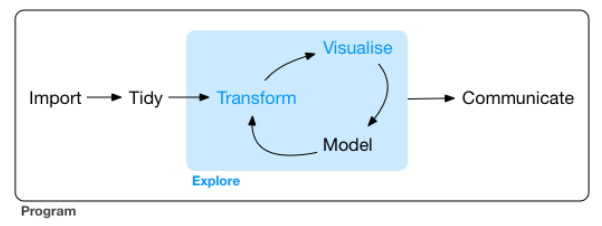
\includegraphics[width=1\linewidth]{imagens/workflow} 

}

\caption{Workflow básico para ciência de dados}\label{fig:unnamed-chunk-3}
\end{figure}

Esse workflow propõe basicamente os seguintes passos:

\begin{itemize}
\tightlist
\item
  Carregar os dados
\item
  Limpar os dados
\item
  Transformar, visualizar e modelar (fase exploratória)
\item
  Comunicar o resultado
\end{itemize}

\section{Linguagens para Ciência de
dados}\label{linguagens-para-ciencia-de-dados}

Para aplicação dessas atividades comuns da ciência de dados, é
necessário dominar as ferramentas corretas. Existem diversas
linguagens/ferramentas: R, Python, SAS, SQL, Matlab, Stata, Aplicações
de BI, etc.

Cabe ao ciêntista de dados avaliar qual a ferramenta mais adequada para
alacançar seus objetivos.

\section{O que é R e por quê devo
aprender?}\label{o-que-e-r-e-por-que-devo-aprender}

R é uma linguagem de programação estatística que vem passando por
diversas evoluções e se tornando cada vez mais uma linguagem de amplos
objetivos. Podemos entender o R também como um conjunto de pacotes e
ferramentas estatísticas, munido de funcões que facilitam sua utilização
desde a criação de simples rotinas até análises de dados complexas com
visualizações bem acabadas.

Segue alguns motivos para aprender R:

\begin{itemize}
\tightlist
\item
  É completamente gratuito e de livre distribuição
\item
  Curva de aprenziado bastante amigável, sendo muito fácil aprender
\item
  Enorme quantidade de tutoriais e ajuda disponíveis gratuitamente na
  internet
\item
  É excelente para criar rotinas e sistematizar tarefas repetitivas
\item
  Amplamente utilizado pela comunidade acadêmica e pelo mercado
\item
  Quantidade enorme de pacotes para diversos tipos de necessidades
\item
  Ótima ferramenta para criar relatórios e gráficos
\end{itemize}

Apenas para exemplificar sua versatilidade, esse eBook e os slides das
aulas foram todos feitos em R.

\section{RStudio}\label{rstudio}

O R puro se apresenta como uma simples ``tela preta'' com uma linha para
inserir comandos. Isso é bastante assustador para quem está começando e
bastante improdutivo para quem já faz uso intensivo da ferramenta.
Flizmente existe o RStudio, ferramenta auxiliar que usaremos durante
todo o curso.

Entenda o RStudio como uma interface gráfica com diversas
funcionalidades que melhoram ainda mais o uso e aprendizado do R. Na
prática, o RStudio facilita muito o dia a dia de trabalho. Portanto,
desde já, ao falarmos em R, falaremos automaticamente no RStudio.

Essa é a ``cara'' do R studio:

\begin{figure}

{\centering 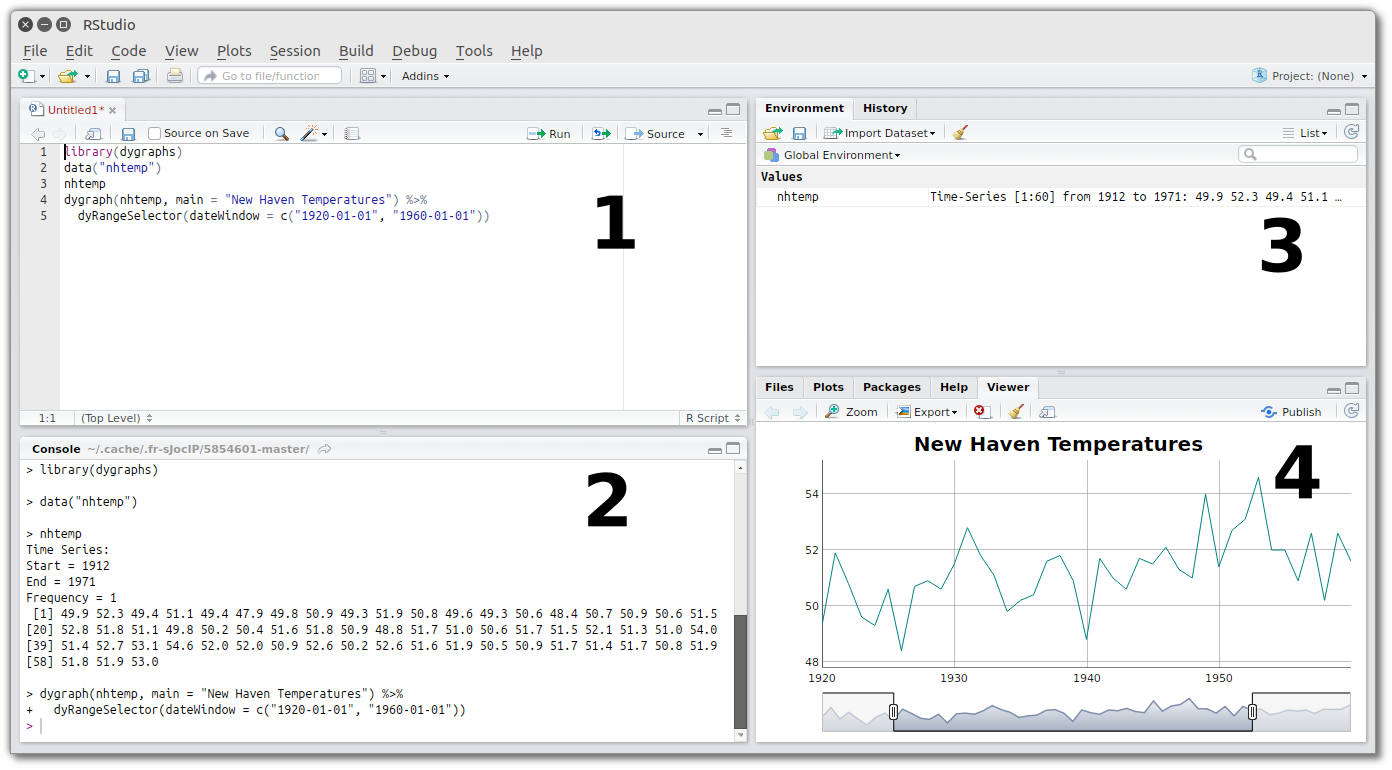
\includegraphics[width=1\linewidth]{imagens/RStudio_001} 

}

\caption{RStudio se divide em 4 partes}\label{fig:unnamed-chunk-4}
\end{figure}

Repare que, além da barra de menu superior, o RStudio é divido em 4
partes principais:

\begin{enumerate}
\def\labelenumi{\arabic{enumi}.}
\tightlist
\item
  Editor de Código

  No editor de código, você poderá escrever e editar os scripts. Script
  nada mais é do que uma sequência de comandos/ordens que serão
  executados em sequência pelo R. O editor do RStudio oferece
  facilidades como organização dos comandos, ``auto-complete'' de
  comandos, destaque da sintaxe dos comandos, etc. Provavelmente é a
  parte que mais utilizaremos.
\end{enumerate}

\begin{enumerate}
\def\labelenumi{\arabic{enumi}.}
\setcounter{enumi}{1}
\tightlist
\item
  Console

  É no console que o R irá mostrar a maioria dos resultados dos
  comandos. Também é possível escrever os comandos diretamente no
  console, sem uso do editor de código. Muito utilizado para testes e
  experimentos rápidos. Por exemplo, um uso rápido do console é chamar a
  ajuda do R usando o comando \texttt{?} (isso mesmo, a interrogação é
  um comando!). Voltaremos a falar desse comando \texttt{?} em breve..
\end{enumerate}

\begin{enumerate}
\def\labelenumi{\arabic{enumi}.}
\setcounter{enumi}{2}
\tightlist
\item
  Environment e History

  No Environment ficarão guardados todos os objetos que forem criados na
  sessão do R. Entenda sessão como o espaço de tempo entre o momento em
  que você inicia o R e o momento que finaliza. Nesse período, tudo que
  você faz usa memória RAM e o processador do computador. E na aba
  History, como você deve imaginar, o RStudio cria um histórico de
  comandos utilizados.
\end{enumerate}

\begin{enumerate}
\def\labelenumi{\arabic{enumi}.}
\setcounter{enumi}{3}
\tightlist
\item
  Files, Plots, Packages, Help e Viewer.

  Nessa janela, estão várias funcionalidades do RStudio. Na aba Files,
  você terá uma navegação de arquivos do seu computador. Também será
  possível definir o diretório de trabalho (você também pode definir
  diretamente no código, mas isto será tratado posteriormente), ou seja,
  o R entende o seu diretório de trabalho como ponto de partida para
  localizar arquivos que sejam chamados no script.
\end{enumerate}

4.1 Aba Plots

A aba Plots trará os gráficos gerados, possibilitando a exportação para
alguns formatos diferentes, como png e pdf.

4.2 Aba Packages

Em Packages, estão listados os pacotes que estão instalados e você pode
verificar quais estão carregados e, caso necessário, poderá carregar
algum pacote necessário para a sua análise. Também é possível instalar e
atualizar pacotes. Novamente, tudo isso é possível fazer diretamente no
código.

4.3 Aba Help

Help o nome já diz tudo. Essa aba será bastante utilizada por você.
Saber usar o help é fundamental para evitar desperdício de tempo. Os
usuários de R, em geral, são bastante solícitos. Entretanto, uma
olhadinha rápida no help pode evitar que você gaste ``créditos''
desnecessariamente.

4.4 Aba Viewer

Por fim, o Viewer. Essa funcionalidade é utilizada para visualizar
localmente conteúdo web. O gráfico da figura está na aba Viewer porque é
uma visualização em javascript, que pode ser adicionada a documentos
htmls gerados usando o RMarkdown ou em aplicações web com suporte do
Shiny.

\section{Buscando Ajuda}\label{buscando-ajuda}

Independente do seu nível de conhecimento, sempre haverá a necessidade
de buscar ajuda. Ou seja, saber procurar ajuda é essencial para
aprimorar seus conhecimentos em ciência de dados. Segue algumas dicas de
como buscar ajuda para sanar dúvidas e resolver problemas em R:

\begin{itemize}
\tightlist
\item
  Sempre procure em inglês, apesar da comunidade R em lingua portuguesa
  ser bem grande, a de lingua inglesa é maior ainda. É muito provável
  que seus problemas e dúvidas já tenham sido sanados.
\item
  Explore bem o help do próprio R.
\item
  Conheça e aprenda a usar o stack overflow, a maior comunidade de ajuda
  técnica da internet.
\end{itemize}

Se mesmo explorando todas as dicas acima não conseguir resolver seu
problema, procure por foruns específicos.

Se você for realizar uma pergunta em algum fórum ou site de perguntas e
respostas, é importante atentar para alguns pontos que deverão ser
informados para que fique mais fácil de alguém te ajudar:

\begin{itemize}
\tightlist
\item
  Versão do R que está usando.
\item
  Sistema Operacional.
\item
  Forneça um exemplo replicável.
\item
  Veja se a sua dúvida já não foi abordada em outro tópico.
\end{itemize}

\section{Exercícios}\label{exercicios}

\begin{enumerate}
\def\labelenumi{\arabic{enumi}.}
\item
  Digite o comando \texttt{R.Version()}. O que acontece?
\item
  Encontre o item de menu \texttt{Help} e descubra como identificar a
  versão do seu RStudio.
\item
  Encontre o item de menu \texttt{Cheatsheets}. O que esse menu oferece?
\item
  Entre no site \url{https://stackoverflow.com} e digite
  \texttt{{[}r{]}} na caixa de busca. O que acontece?
\end{enumerate}

\chapter{Conceitos Básicos}\label{conceitos-basicos}

Entenda o R como uma grande calculadora científica cheia de botões, mas,
ao invés de apertar os botões, você irá escrever os comandos. Ou seja,
``aprender R'' significa se familizarizar com os comandos e saber quando
usá-los. Todos os comandos são baseados em inglês e seus nomes
normalmente dão dicas do seu uso.

\section{Console}\label{console}

O console é uma das 4 partes principais do RStudio. Lá é onde você vai
digitar suas ordens (comandos) e é onde o R vai ``responder''. Para que
o R possa interpretar correntamente, será necessário que você conheça a
sintaxe da linguagem e a escrita correta dos comandos.

Olhando para o console você irá ver o símbolo \texttt{\textgreater{}}.
Esse símbolo indica a linha onde você deve inserir os comandos. Clique
nesse símbolo para posicionar o cursor na linha de comandos e digite seu
primeiro comando em R: \texttt{2\ *\ 3}. Digite e aperte \emph{enter}.
Você verá o seguinte resultado:

\begin{verbatim}
## [1] 6
\end{verbatim}

Além de outras funcionalidades mais interessantes, o R é como uma grande
calculadora científica. Para entender esse conceito melhor, vamos
exercitar um pouco no console de comandos. Digite um por um dos
seguintes comandos e acompanhe os resultados:

\begin{Shaded}
\begin{Highlighting}[]
\DecValTok{7} \OperatorTok{*}\StringTok{ }\DecValTok{9} \OperatorTok{+}\StringTok{ }\DecValTok{2} \OperatorTok{*}\StringTok{ }\DecValTok{6}
\FloatTok{2.5} \OperatorTok{*}\StringTok{ }\DecValTok{4}
\NormalTok{(}\DecValTok{50} \OperatorTok{+}\StringTok{ }\DecValTok{7}\NormalTok{)}\OperatorTok{/}\NormalTok{(}\DecValTok{8} \OperatorTok{*}\StringTok{ }\NormalTok{(}\DecValTok{3} \OperatorTok{-}\StringTok{ }\DecValTok{5}\OperatorTok{/}\DecValTok{2}\NormalTok{))}
\DecValTok{3} \OperatorTok{^}\StringTok{ }\DecValTok{4}
\end{Highlighting}
\end{Shaded}

Repare que, na medida em que for executando os comandos, o R vai
respondendo. Esse é o comportamento básico do console. Muito utilizado
para obter resultados rápidos de comandos específicos.

Um boa dica é que o R guarda um histórico dos comandos que você executou
por último, basta apertar a seta para cima no teclado e ver os comandos
executados anterioremente.

\section{Scripts}\label{scripts}

Enquanto no console seus comandos são executados na medida que você os
``envia'' com o \emph{enter}, em um script você ordena a execução de uma
sequência de comandos escritos previamente, um seguido do outro. Scripts
são escritos no editor de códigos do RStudio. Para entender melhor,
localize o editor de códigos no RStudio e copie os mesmos comandos
anteriores executados no console. No editor de códigos, a ordem para
execuão dos comandos não é o \emph{enter}. Para executá-los, clique em
\textbf{\emph{Source}}, no canto superior direito da área do editor de
códigos. Repare bem pois há uma setinha escura que revelará duas opções
de \emph{Source} (execução do script): \textbf{\emph{Source}}, e
\textbf{\emph{Source With Echo}}. A diferença entre as duas opções é que
a primeira executa mas não exibe as respostas no console, a segunda
executa mostrando as respostas. A primeira opção será útil em outros
casos de scripts muito grandes ou outras situações que não convém
``poluir'' o console com um monte de mensagens.

Há um atalho de teclado para o \textbf{\emph{Source}}: \emph{ctrl +
shift + enter}. Aprenda esse atalho, pois você usará muito mais o editor
de códigos do que o console para executar os passos da sua análise.

Agora posicione o cursos do mouse com um clique em apenas um dos
comandos do seu script. Em seguida, clique no ícone \textbf{\emph{Run}}
também no canto superior na área do editor de códigos. Repare que dessa
vez o R executou apenas um comando, o que estava na linha selecionada.
Esse tipo de execução também é bastante útil, mas esteja atento, pois é
muito comum que comandos em sequência dependam da execução de comandos
anteriores para funcionar corretamente.

Há um atalho de teclado para o \textbf{\emph{Run}}: \emph{ctrl + enter}.
Aprenda esse atalho, ele também é muito importante e muito utilizado.

\subsection{Salvando Scripts}\label{salvando-scripts}

Ao digitar seus comandos no console, o máximo que você consegue
recuperar são os comandos anteriores usando a seta para cima. Já no
editor de códigos, existe a possibilidade de salvar os seus scripts para
continuar em outro momento ou em outro computador, preservar trabalhos
passados ou compartilhar seus códigos com a equipe.

Um script em R tem a extensão (terminação) \texttt{.R}. Se você tiver o
RStudio instalado e der dois clicks em um arquivo com extesão
\texttt{.R}, o windows abrirá direto no RStudio.

Ainda utilizando os comandos digitados no editor de códigos, vá em
\textbf{\emph{File \textgreater{} Save}}. Escolha um local e um nome
para seu script e confirme no botão \textbf{\emph{Save}}. Lembre-se
sempre de ser organizado utilizando pastas para os diferentes projetos e
nomes explicativos. Para salvar mais rapidamente, utilize o atalho
\textbf{\emph{ctrl + S}}

\subsection{Comentários de Código}\label{comentarios-de-codigo}

Ao utilizar o símbolo \texttt{\#} em uma linha, você está dizendo para o
R ignorar aquela linha, pois trata-se de um comentário.

Clique na primeira linha do seu script, aperte \emph{enter} para
adicionar uma linha a mais e digite
\texttt{\#\ Meu\ primeiro\ comentário\ de\ código!}. Repare que a cor do
comentário é diferente. Execute novamente seu script com o
\emph{\emph{Source (ctrl + shift + enter)}} e veja que nada mudou na
execução. A título de experimento, retire o símbolo \texttt{\#} e
mantenha o texto do comentário. Execute novamente. O R tenta interpretar
essa linha como comando. Já que ele não conseguiu entender, será exibida
uma mensagem de erro no console.

O símbolo de comentário também é muito útil para suprimir linhas de
código para testar determinados comportamentos. Para exemplificar,
adicione o símbolo \texttt{\#} em qualquer uma das linhas com as
operações e veja que ela não será mais executada, será ignorada pois foi
entendida pelo R como um simples comentário de código.

\section{Objetos (Variáveis)}\label{objetos-variaveis}

Para que o R deixe de ser uma simples calculadora, será necessário
aprender, dentre outras coisas, o uso de variáveis. Se você já tem
alguma noção de estatística, provavelmente já tem a intuição do que vem
a ser uma variável para uma linguagem de programação. No contexto do R,
vamos entender variável como um objeto, ou seja, como uma estrutura pré
definida que vai ``receber'' algum valor. Sendo mais técnico, objeto (ou
variável) é um pequeno espaço na memória do seu computador onde o R vai
armazenar um valor ou resultado de um comando utilizando um nome que
você mesmo definiu.

Conhecer os tipos de objetos do R é fundamental. Para criar objetos se
utiliza o símbolo \texttt{\textless{}-}. Esse provavelmente é o símbolo
que você mais vai ver daqui para frente.

Execute, no console ou no editor de códigos, o seguinte comando
\texttt{x\ \textless{}-\ 15}. Pronto. Agora o nome \texttt{x} representa
o valor \texttt{15}. Para comprovar execute apenas o nome do objeto
\texttt{x}, o R irá mostrar o conteúdo dele. A partir de então, você
poderá utilizar esse objeto como se fosse o valor 15. Experimente os
seguintes resultados:

\begin{Shaded}
\begin{Highlighting}[]
\NormalTok{x }\OperatorTok{+}\StringTok{ }\DecValTok{5}
\NormalTok{x }\OperatorTok{*}\StringTok{ }\NormalTok{x }\OperatorTok{/}\StringTok{ }\DecValTok{2}
\DecValTok{2} \OperatorTok{^}\StringTok{ }\NormalTok{x}
\NormalTok{y <-}\StringTok{ }\NormalTok{x }\OperatorTok{/}\StringTok{ }\DecValTok{3}
\end{Highlighting}
\end{Shaded}

De uma boa lida em \emph{Dicas e boas práticas para um código
organizado} para aprender a organizar seus objetos e funções da melhor
maneira possível.

Todos objetos que você criar estarão disponíveis na aba
\textbf{\emph{Environment}}.

O RStudio possui a função de \emph{auto complete}. Digite as primeiras
letras de um objeto (ou função) que você criou e em seguida use o atalho
\textbf{\emph{ctrl + barra de espaço}}. O RStudio irá listar tudo que
começar com essas letras. Selecione alguma e aperte \emph{enter} para
escrevê-la no editor de códigos.

\section{Funções}\label{funcoes}

Entenda função como uma sequência de comandos preparados para serem
usados de forma simples e facilitar sua vida. Funções são usadas para
tudo que você possa imaginar: cálculos mais complexos, estatística,
análise de dados, manipulação de dados, gráficos, relatórios, etc. Assim
que você instala o R ele já vem com várias funções prontas para uso. A
partir de agora chamaremos esse conjunto de funções que já vem por
padrão com o R de \emph{R Base}.

Claro que as funções do R base não serão suficientes para resolver todos
os problemas que você vai encontrar pela frente. Nesse sentido o R
também mostra outro ponto forte. Você pode instalar conjuntos extras de
funções mais específicas de maneira muito simples: usando pacotes.

Funcões do R base.

\begin{Shaded}
\begin{Highlighting}[]
\NormalTok{raiz.quadrada <-}\StringTok{ }\KeywordTok{sqrt}\NormalTok{(}\DecValTok{16}\NormalTok{) }\CommentTok{# função para calcular raiz quadrada}

\KeywordTok{round}\NormalTok{(}\FloatTok{5.3499999}\NormalTok{, }\DecValTok{2}\NormalTok{) }\CommentTok{# função para arredondamento}
\end{Highlighting}
\end{Shaded}

Uma função tem dois elementos básicos: o nome e o(s) parâmetro(s)
(também chamados de argumentos). Por exemplo, a função \texttt{log(10)}
possui o nome \texttt{log()} e apenas um parâmetro que é o número que
você quer calcular o log. Já a função \texttt{round()} possui dois
parâmetros, o número que você quer arredondar e a quantidade de dígitos
para arredondamento.

Quando você usa uma função, você pode informar os parâmetros de duas
formas: sequencialmente sem explicitar o nome dos parâmetros, ou na
ordem que quiser explicitando o nome dos parâmetros. Veja o exemplo a
seguir:

\begin{Shaded}
\begin{Highlighting}[]
\KeywordTok{round}\NormalTok{(}\FloatTok{5.3499999}\NormalTok{, }\DecValTok{2}\NormalTok{)}
\CommentTok{# o mesmo que:}
\KeywordTok{round}\NormalTok{(}\DataTypeTok{digits =} \DecValTok{2}\NormalTok{, }\DataTypeTok{x =} \FloatTok{5.3499999}\NormalTok{)}
\end{Highlighting}
\end{Shaded}

Para saber como informar os parâmetros corretamente, utilize o comando
\texttt{?} (ou coloque o cursor no nome da função e pressione F1) para
ver a documentação de funções, ou seja, conhecer para que ela serve,
entender cada um dos seus parâmetros e ver exemplos de uso.

\begin{Shaded}
\begin{Highlighting}[]
\NormalTok{?round}
\NormalTok{?rnorm}
\NormalTok{??inner_join }\CommentTok{# procurar ajuda de funções que não estão "instaladas" ainda}
\end{Highlighting}
\end{Shaded}

Vale comentar que é possível informar objetos nos parâmetros das
funções.

\begin{Shaded}
\begin{Highlighting}[]
\NormalTok{x <-}\StringTok{ }\FloatTok{3.141593}
\KeywordTok{round}\NormalTok{(x, }\DecValTok{3}\NormalTok{)}
\end{Highlighting}
\end{Shaded}

\begin{verbatim}
## [1] 3.142
\end{verbatim}

\begin{Shaded}
\begin{Highlighting}[]
\KeywordTok{ceiling}\NormalTok{(x)}
\end{Highlighting}
\end{Shaded}

\begin{verbatim}
## [1] 4
\end{verbatim}

\begin{Shaded}
\begin{Highlighting}[]
\KeywordTok{floor}\NormalTok{(x)}
\end{Highlighting}
\end{Shaded}

\begin{verbatim}
## [1] 3
\end{verbatim}

Observe algumas das principais funções para estatísticas básicas no R:

\begin{longtable}[]{@{}lc@{}}
\toprule
Função R & Estatística\tabularnewline
\midrule
\endhead
\texttt{sum()} & Soma de valores\tabularnewline
\texttt{mean()} & Média\tabularnewline
\texttt{var()} & Variancia\tabularnewline
\texttt{median()} & Mediana\tabularnewline
\texttt{summary()} & Resumo Estatístico\tabularnewline
\texttt{quantile()} & Quantis\tabularnewline
\bottomrule
\end{longtable}

\section{Pacotes}\label{pacotes}

Como dito antes, pacotes são conjuntos extras de funções que podem ser
instalados além do R base. Existe pacotes para auxiliar toda linha de
estudo você imaginar: estatística, econometria, ciências sociais,
medicina, biologia, gráficos, machine learning, etc.

Caso você precise de algum pacote mais específico, procure no google
pelo tema que você precisa, encontre o nome do pacote e instale
normalmente.

\href{https://cran.r-project.org/web/packages/available_packages_by_name.html}{Nesse
link} você pode ver uma lista de todos os pacotes disponíveis no
repositório central. Além desses, ainda existe a possibilidade de
instalar pacotes ``não oficiais'', que ainda não fazem parte de um
repositório central.

Para instalar um pacote, execute o seguinte comando:

\begin{Shaded}
\begin{Highlighting}[]
\KeywordTok{install.packages}\NormalTok{(}\StringTok{"dplyr"}\NormalTok{) }\CommentTok{# instala um famoso pacote de manipulação de dados}
\end{Highlighting}
\end{Shaded}

Uma vez instalado, esse pacote estará disponível para uso sempre que
quiser, sem necessidade de instalar novamente. Mas sempre que iniciar um
código novo, você precisará carregá-lo na memória. Para isso, use o
seguinte comando:

\begin{Shaded}
\begin{Highlighting}[]
\KeywordTok{library}\NormalTok{(dplyr)}
\end{Highlighting}
\end{Shaded}

Para instalar um pacote você precisa informar o nome entre aspas
install.packages(``readxl''), caso contrário não vai funcionar. Porém,
para carregar o pacote em memória, você pode usar com ou sem aspas
library(readxl) ou library(``readxl''), ambas as formas funcionam.

\section{Boas práticas}\label{boas-praticas}

Rapidamente você irá perceber que quanto mais organizado e padronizado
você mantiver seus códigos, melhor para você e para sua equipe.

Existem dois guias de boas práticas bastante famosos na comunidade do R.
Um sugerido pelo Hadley Wickham e outro por uma equipe do google.

Dentre as dicas de boa prática, algumas são as mais importantes, como
por exemplo, não use acentos e caracteres especiais. Outro ponto
importante, o R não aceita variáveis que comecem com números. Você pode
até usar números no meio do nome, mas nunca começar com números.

O principal de tudo é, seja qual for o padrão que você preferir, use um
padrão e seja consistente.

\begin{itemize}
\tightlist
\item
  Guia sugerido Hadley Wickham: \url{http://adv-r.had.co.nz/Style.html}
\end{itemize}

\_ Guia sugerido pelo Google:
\url{https://google.github.io/styleguide/Rguide.xml}

\section{Tidyverse}\label{tidyverse}

Como já dito, eventualmente as funções do R base não é suficiente ou
simplesmente não fornecem maneira mais fácil de resolver um problema.
Nesse curso utilizaremos o Tidyverse: uma coleção de pacotes R
cuidadosamente desenhados para atuar no workflow comum da ciência de
dados: importação, manipulação, exploração e visualização de dados. Uma
vez carregado, esse pacote disponibiliza todo o conjunto de ferramentas
de outros pacotes importantes: ggplot2, tibble, tidyr, readr, purrr e
dplyr. Oportunamente detalharemos cada um deles.

O Tidyverse foi idealizado, dentre outros responsáveis, por Hadley
Wickham, um dos maiores colaboradores da comunidade R. Se você não o
conhece e pretende seguir em frente com o R, certamente vai ouvir falar
muito dele. Recomendamos segui-lo nas redes sociais para ficar por
dentro das novidades do Tidyverse.

\section{Exercícios}\label{exercicios-1}

\begin{enumerate}
\def\labelenumi{\arabic{enumi}.}
\item
  Quais as principais diferenças entre um script e o console?
\item
  Digite \texttt{?dplyr} o que acontece? E se digitar \texttt{??dplyr}?
  para que serve esse pacote?
\item
  Para que serve a função \texttt{rnorm()}? Quais os seus
  parâmetros/atributos?
\item
  Para que serve a função \texttt{rm()}? Quais os seus
  parâmetros/atributos?
\end{enumerate}

\chapter{Lendo os dados}\label{lendo-os-dados}

Após o entendimento do problema/projeto que irá resolver com ciência de
dados será necessário fazer com que o R leia os dados. Seja lá qual for
o assunto do projeto, é muito importante garantir uma boa fonte de
dados. Dados ruins, inconsistentes, não confiáveis ou mal formatados
podem gerar muita dor de cabeça para o analista.

\section{Tipos de Estrutura dos
Dados}\label{tipos-de-estrutura-dos-dados}

Os dados podem ser apresentados de diversas maneiras, não existe um
padrão único para difusão ou divulgação. Sendo assim, é bom que você
esteja preparado para lidar com qualquer tipo de estrutura de dados.

Existem diversas classificações de estrutura de dados. Vamos utilizar
uma classificação mais geral que diz respeito a como os dados são
disponibilizados. Sendo assim, podemos classificar os dados em 3 grandes
tipos quanto à sua estrutura ou forma: dados estruturados,
semiestruturados e não estruturados.

\subsection{Dados Estruturados}\label{dados-estruturados}

Talvez seja o formato de dados mais fácil de se trabalhar no R. São
conjuntos de informações organizadas em colunas (atributos, variáveis,
features, etc.) e linhas (registros, itens, observações, etc.). São
dados mais comumente encontrados diretamente em bancos de dados,
arquivos com algum tipo de separação entre as colunas, Excel, arquivos
com campos de tamanho fixo, etc.

\subsection{Dados Não Estruturados}\label{dados-nao-estruturados}

Como o nome diz, não tem um estrutura previsível, ou seja, cada conjunto
e informações possui uma forma única. Geralmente são arquivos com forte
teor textual. Não podemos dizer que são dados ``desorganizados'', e sim
que são organizações particulares para cada conjunto de informações.
Podemos citar, por exemplo, emails, twitters, PDFs, imagens, vídeos,
etc.

Analisar esse tipo de dado é muito mais complexo e exige conhecimento
avançado em mineração de dados. Apesar disso, é o tipo de dados mais
abundante na realidade.

\subsection{Dados Semiestruturados}\label{dados-semiestruturados}

São dados que também possuem uma organização fixa, porém, não seguem o
padrão de estrutura linha/coluna, ou seja, é uma estrutura mais complexa
e flexível, geralmente hierárquica, estruturada em tags ou marcadores de
campos. São exemplos de arquivos semiestruturados: JSON, XML, HTML,
YAML, etc. É o formato mais usado em troca de dados pela internet e
consumo de APIs (Application programming interface). Dados
semiestruturados algumas vezes são facilmente transformados em dados
estruturados.

\section{Definindo o Local dos Dados}\label{definindo-o-local-dos-dados}

O R sempre trabalha com o conceito de \emph{Working direcotry}, ou seja,
uma pasta de trabalho onde ele vai ``ler'' e ``escrever'' os dados. Para
verificar qual o diretório o R está ``olhando'', utilize o seguinte
comando:

\begin{Shaded}
\begin{Highlighting}[]
\KeywordTok{getwd}\NormalTok{() }\CommentTok{#Get Working Directory}
\end{Highlighting}
\end{Shaded}

Para informar ao R em qual pasta ele deve ler os arquivos, utilizamos o
comando \emph{set working directory}, que muda o diretório padrão do R
para leitura e escrita:

\begin{Shaded}
\begin{Highlighting}[]
\KeywordTok{setwd}\NormalTok{(}\StringTok{'D:/caminho/do/arquivo/arquivo.csv'}\NormalTok{)}
\end{Highlighting}
\end{Shaded}

\section{Pacote para leitura dos
dados}\label{pacote-para-leitura-dos-dados}

O R base possui funções para leitura dos principais tipos de arquivos.
Um outro pacote específico e muito bom para isso é o \texttt{readr}. O
Tidyverse inclui o carregamento do \texttt{readr}.

O R é capaz de ler diversos tipos de arquivos: csv (Comma-Separated
Values), excel, arquivos serparados por delimitadores, colunas de
tamanho fixo, etc. Talvez o tipo de arquivo (estruturado) mais comum
hoje em dia, e mais simples de trabalhar, seja o csv. Começaremos a
importar dados com arquivos csv.

\begin{Shaded}
\begin{Highlighting}[]
\KeywordTok{library}\NormalTok{(tidyverse) }\CommentTok{# já carrega o readr}
\CommentTok{#ou}
\KeywordTok{library}\NormalTok{(readr)}
\end{Highlighting}
\end{Shaded}

Vamos importar um csv chamado \texttt{senado.csv}. Caso o arquivo esteja
em seu working directory (\texttt{getwd()}), basta passar apenas o nome
do arquivo para a função, caso contrário será necessário informar todo o
caminho até a pasta do arquivo. Usamos o read\_csv() para fazer isso.

\begin{Shaded}
\begin{Highlighting}[]
\NormalTok{senado <-}\StringTok{ }\KeywordTok{read_csv}\NormalTok{(}\StringTok{"senado.csv"}\NormalTok{)}
\end{Highlighting}
\end{Shaded}

Esse comando simplesmente carrega o conteúdo do arquivo
\texttt{senado.csv} para o objeto (variável) senado. Após o
carregamento, começaremos a investigar o conteúdo desse objeto: os
dados.

O \texttt{head} e o \texttt{tail} são funções para ver a ``cabeça'' e o
``rabo'' dos seus dados, ou seja, o começo das amostras e fim das
amostras. É muito importante sempre dar uma olhada na ``cara'' dos dados
após o carregamento. Essa olhada ajuda a identificar erros básicos no
carregamento, possibilitando ajustes o quanto antes, impedindo que esses
erros se propaguem. Repare que na primeira linha temos os nomes das
colunas e em seguida os registros.

\begin{Shaded}
\begin{Highlighting}[]
\KeywordTok{head}\NormalTok{(senado)}
\end{Highlighting}
\end{Shaded}

\begin{verbatim}
## # A tibble: 6 x 15
##   VoteNumber  SenNumber     SenatorUpper  Vote Party GovCoalition State
##        <int>      <chr>            <chr> <chr> <chr>        <lgl> <chr>
## 1    2007001 PRS0002/07    FLEXA RIBEIRO     S  PSDB        FALSE    PA
## 2    2007001 PRS0002/07  ARTHUR VIRGILIO     S  PSDB        FALSE    AM
## 3    2007001 PRS0002/07      FLAVIO ARNS     N    PT         TRUE    PR
## 4    2007001 PRS0002/07 MARCELO CRIVELLA     S   PRB         TRUE    RJ
## 5    2007001 PRS0002/07      JOAO DURVAL     N   PDT        FALSE    BA
## 6    2007001 PRS0002/07       PAULO PAIM     S    PT         TRUE    RS
## # ... with 8 more variables: FP <int>, Origin <int>, Contentious <int>,
## #   PercentYes <dbl>, IndGov <chr>, VoteType <int>, Content <chr>,
## #   Round <int>
\end{verbatim}

\begin{Shaded}
\begin{Highlighting}[]
\KeywordTok{tail}\NormalTok{(senado)}
\end{Highlighting}
\end{Shaded}

\begin{verbatim}
## # A tibble: 6 x 15
##   VoteNumber  SenNumber       SenatorUpper  Vote Party GovCoalition State
##        <int>      <chr>              <chr> <chr> <chr>        <lgl> <chr>
## 1    2010027 PLC0010/10       EDISON LOBAO     S  PMDB         TRUE    MA
## 2    2010027 PLC0010/10    EDUARDO SUPLICY     S    PT         TRUE    SP
## 3    2010027 PLC0010/10 JARBAS VASCONCELOS     N  PMDB         TRUE    PE
## 4    2010027 PLC0010/10     MARISA SERRANO     S  PSDB        FALSE    MS
## 5    2010027 PLC0010/10 EPITACIO CAFETEIRA     S   PTB        FALSE    MA
## 6    2010027 PLC0010/10      INACIO ARRUDA     S PCdoB         TRUE    CE
## # ... with 8 more variables: FP <int>, Origin <int>, Contentious <int>,
## #   PercentYes <dbl>, IndGov <chr>, VoteType <int>, Content <chr>,
## #   Round <int>
\end{verbatim}

Outros comandos muito importantes para começar a investigar os dados é o
\texttt{str()}o \texttt{class()} e o \texttt{summary()}

Para verificar o tipo do objeto, ou seja, sua classe:

\begin{Shaded}
\begin{Highlighting}[]
\KeywordTok{class}\NormalTok{(senado)}
\end{Highlighting}
\end{Shaded}

\begin{verbatim}
## [1] "tbl_df"     "tbl"        "data.frame"
\end{verbatim}

Para verificar a estrutura do objeto, ou seja, seus campos (quando
aplicável):

\begin{Shaded}
\begin{Highlighting}[]
\KeywordTok{str}\NormalTok{(senado) }\CommentTok{#STRucture}
\end{Highlighting}
\end{Shaded}

\begin{verbatim}
## Classes 'tbl_df', 'tbl' and 'data.frame':    9262 obs. of  15 variables:
##  $ VoteNumber  : int  2007001 2007001 2007001 2007001 2007001 2007001 2007001 2007001 2007001 2007001 ...
##  $ SenNumber   : chr  "PRS0002/07" "PRS0002/07" "PRS0002/07" "PRS0002/07" ...
##  $ SenatorUpper: chr  "FLEXA RIBEIRO" "ARTHUR VIRGILIO" "FLAVIO ARNS" "MARCELO CRIVELLA" ...
##  $ Vote        : chr  "S" "S" "N" "S" ...
##  $ Party       : chr  "PSDB" "PSDB" "PT" "PRB" ...
##  $ GovCoalition: logi  FALSE FALSE TRUE TRUE FALSE TRUE ...
##  $ State       : chr  "PA" "AM" "PR" "RJ" ...
##  $ FP          : int  2 2 2 2 2 2 2 2 2 2 ...
##  $ Origin      : int  11 11 11 11 11 11 11 11 11 11 ...
##  $ Contentious : int  0 0 0 0 0 0 0 0 0 0 ...
##  $ PercentYes  : num  85.5 85.5 85.5 85.5 85.5 ...
##  $ IndGov      : chr  "S" "S" "S" "S" ...
##  $ VoteType    : int  1 1 1 1 1 1 1 1 1 1 ...
##  $ Content     : chr  "Creates the Senate Commission of Science, Technology, Innovation, Communication, and Information Technology (CCT)." "Creates the Senate Commission of Science, Technology, Innovation, Communication, and Information Technology (CCT)." "Creates the Senate Commission of Science, Technology, Innovation, Communication, and Information Technology (CCT)." "Creates the Senate Commission of Science, Technology, Innovation, Communication, and Information Technology (CCT)." ...
##  $ Round       : int  1 1 1 1 1 1 1 1 1 1 ...
##  - attr(*, "spec")=List of 2
##   ..$ cols   :List of 15
##   .. ..$ VoteNumber  : list()
##   .. .. ..- attr(*, "class")= chr  "collector_integer" "collector"
##   .. ..$ SenNumber   : list()
##   .. .. ..- attr(*, "class")= chr  "collector_character" "collector"
##   .. ..$ SenatorUpper: list()
##   .. .. ..- attr(*, "class")= chr  "collector_character" "collector"
##   .. ..$ Vote        : list()
##   .. .. ..- attr(*, "class")= chr  "collector_character" "collector"
##   .. ..$ Party       : list()
##   .. .. ..- attr(*, "class")= chr  "collector_character" "collector"
##   .. ..$ GovCoalition: list()
##   .. .. ..- attr(*, "class")= chr  "collector_logical" "collector"
##   .. ..$ State       : list()
##   .. .. ..- attr(*, "class")= chr  "collector_character" "collector"
##   .. ..$ FP          : list()
##   .. .. ..- attr(*, "class")= chr  "collector_integer" "collector"
##   .. ..$ Origin      : list()
##   .. .. ..- attr(*, "class")= chr  "collector_integer" "collector"
##   .. ..$ Contentious : list()
##   .. .. ..- attr(*, "class")= chr  "collector_integer" "collector"
##   .. ..$ PercentYes  : list()
##   .. .. ..- attr(*, "class")= chr  "collector_double" "collector"
##   .. ..$ IndGov      : list()
##   .. .. ..- attr(*, "class")= chr  "collector_character" "collector"
##   .. ..$ VoteType    : list()
##   .. .. ..- attr(*, "class")= chr  "collector_integer" "collector"
##   .. ..$ Content     : list()
##   .. .. ..- attr(*, "class")= chr  "collector_character" "collector"
##   .. ..$ Round       : list()
##   .. .. ..- attr(*, "class")= chr  "collector_integer" "collector"
##   ..$ default: list()
##   .. ..- attr(*, "class")= chr  "collector_guess" "collector"
##   ..- attr(*, "class")= chr "col_spec"
\end{verbatim}

Para verificar estatísticas básicas do objeto (média, mediana, quantis,
mínimo, máximo\ldots{} quando aplicável):

\begin{Shaded}
\begin{Highlighting}[]
\KeywordTok{summary}\NormalTok{(senado)}
\end{Highlighting}
\end{Shaded}

\begin{verbatim}
##    VoteNumber       SenNumber         SenatorUpper      
##  Min.   :2007001   Length:9262        Length:9262       
##  1st Qu.:2008006   Class :character   Class :character  
##  Median :2009003   Mode  :character   Mode  :character  
##  Mean   :2008483                                        
##  3rd Qu.:2009048                                        
##  Max.   :2010027                                        
##      Vote              Party           GovCoalition       State          
##  Length:9262        Length:9262        Mode :logical   Length:9262       
##  Class :character   Class :character   FALSE:3480      Class :character  
##  Mode  :character   Mode  :character   TRUE :5782      Mode  :character  
##                                                                          
##                                                                          
##                                                                          
##        FP            Origin        Contentious        PercentYes     
##  Min.   :1.000   Min.   : 1.000   Min.   :0.00000   Min.   :  2.174  
##  1st Qu.:2.000   1st Qu.: 1.000   1st Qu.:0.00000   1st Qu.: 66.667  
##  Median :2.000   Median : 2.000   Median :0.00000   Median : 96.078  
##  Mean   :1.878   Mean   : 2.595   Mean   :0.01781   Mean   : 82.509  
##  3rd Qu.:2.000   3rd Qu.: 4.000   3rd Qu.:0.00000   3rd Qu.: 98.148  
##  Max.   :2.000   Max.   :11.000   Max.   :1.00000   Max.   :100.000  
##     IndGov             VoteType       Content              Round      
##  Length:9262        Min.   :1.000   Length:9262        Min.   :1.000  
##  Class :character   1st Qu.:1.000   Class :character   1st Qu.:1.000  
##  Mode  :character   Median :1.000   Mode  :character   Median :1.000  
##                     Mean   :1.159                      Mean   :1.358  
##                     3rd Qu.:1.000                      3rd Qu.:2.000  
##                     Max.   :2.000                      Max.   :4.000
\end{verbatim}

Acontece que nem sempre o separador será o \texttt{;}, típico do csv.
Nesse caso será necessário usar o \texttt{read\_delim()}, onde você pode
informar qualquer tipo de separador. Outro tipo de arquivo bastante
comum é o de colunas com tamanho fixo (fixed width), ou também conhecido
como colunas posicionais. Nesse caso será necessário usar o
\texttt{read\_fwf()} informando o tamanho de cada coluna.

Exemplo:

\begin{Shaded}
\begin{Highlighting}[]
\CommentTok{#lendo arquivo com delimitador #}
\KeywordTok{read_delim}\NormalTok{(}\StringTok{'caminho/do/arquivo/arquivo_separado_por#.txt'}\NormalTok{, }\DataTypeTok{delim =} \StringTok{'#'}\NormalTok{)}

\CommentTok{#lendo arquivo de coluna fixa}
\CommentTok{#coluna 1 de tamanho 5, coluna 2 de tamanho 2 e coluna 3 de tamanho 10}
\KeywordTok{read_fwf}\NormalTok{(}\StringTok{'caminho/do/arquivo/arquivo_posicional.txt'}\NormalTok{, }\DataTypeTok{col_positions =} \KeywordTok{fwf_widths}\NormalTok{(}\KeywordTok{c}\NormalTok{(}\DecValTok{5}\NormalTok{, }\DecValTok{2}\NormalTok{, }\DecValTok{10}\NormalTok{), }\KeywordTok{c}\NormalTok{(}\StringTok{"col1"}\NormalTok{, }\StringTok{"col2"}\NormalTok{, }\StringTok{"col3"}\NormalTok{)))}
\end{Highlighting}
\end{Shaded}

No capítulo a seguir entenderemos melhor os tipos de objeto mais comuns
no R.

\section{Exercícios:}\label{exercicios-2}

\begin{enumerate}
\def\labelenumi{\arabic{enumi}.}
\item
  Leia o arquivo \texttt{TA\_PRECOS\_MEDICAMENTOS.csv} cujo separador é
  uma barra \texttt{\textbar{}}.
\item
  Leia o arquivo de colunas fixas \texttt{fwf-sample.txt} cuja primeira
  coluna (nomes) tem tamanho 20, a segunda (estado) tem tamanho 10 e a
  terceira (codigo) tem tamanho 12.
\item
  Investigue os parâmetros das funções de leitura do R base:
  \texttt{read.csv()}, \texttt{read.delim()} e \texttt{read.fwf()}.
  Notou diferenças das funções do \texttt{readr}?
\end{enumerate}

\chapter{Manipulando os dados}\label{manipulando-os-dados}

Após obter uma boa fonte de dados e carregá-los para poder trabalhá-los
no R, você certamente precisará realizar algumas limpezas e manipulações
para que os dados estejam no ponto ideal para as fases finais de uma
análise: execução de modelos econométricos, visualizações de dados,
tabelas agregadas, relatórios, etc. A realidade é que na prática os
dados nunca estarão do jeito que você de fato precisa. Portanto, é
fundamental dominar técnicas de manipulação de dados.

Vamos entender a manipulação de dados como o ato de transformar,
reestruturar, limpar, agregar, juntar dados. Para se ter uma noção da
importância dessa fase, alguns estudiosos da área de ciência de dados
costumam afirmar que 80\% do trabalho é encontrar uma boa fonte de
dados, limpar e preparar os dados, sendo que os 20\% restantes seriam o
trabalho de aplicar modelos e realizar alguma análise propriamente dita.

\begin{quote}
80\% of data analysis is spent on the process of cleaning and preparing
the data (Dasu and Johnson, 2003).
\end{quote}

\begin{quote}
Data preparation is not just a first step, but must be repeated many
over the course of analysis as new problems come to light or new data is
collected (Hadley Wickham).
\end{quote}

\section{Tipos de Variáveis e
Colunas}\label{tipos-de-variaveis-e-colunas}

Existem diversos tipos de objetos, e cada tipo ``armazena'' um conteúdo
diferente, desde tabelas de dados recém carregados, textos, números, ou
simplesmente a afirmação de verdadeiro ou falso (boleano).

\begin{Shaded}
\begin{Highlighting}[]
\NormalTok{inteiro <-}\StringTok{ }\DecValTok{928}
\NormalTok{outro.inteiro <-}\StringTok{ }\FloatTok{5e2}
\NormalTok{decimal <-}\StringTok{ }\FloatTok{182.93}
\NormalTok{caracter <-}\StringTok{ 'exportação'}
\NormalTok{logico <-}\StringTok{ }\OtherTok{TRUE}
\NormalTok{outro.logico <-}\StringTok{ }\OtherTok{FALSE}
\end{Highlighting}
\end{Shaded}

Repare nas atribuições acima. Vamos usar a função \texttt{class()} para
ver o tipo de cada uma:

\begin{Shaded}
\begin{Highlighting}[]
\KeywordTok{class}\NormalTok{(inteiro)}
\end{Highlighting}
\end{Shaded}

\begin{verbatim}
## [1] "numeric"
\end{verbatim}

\begin{Shaded}
\begin{Highlighting}[]
\KeywordTok{class}\NormalTok{(outro.inteiro)}
\end{Highlighting}
\end{Shaded}

\begin{verbatim}
## [1] "numeric"
\end{verbatim}

\begin{Shaded}
\begin{Highlighting}[]
\KeywordTok{class}\NormalTok{(decimal)}
\end{Highlighting}
\end{Shaded}

\begin{verbatim}
## [1] "numeric"
\end{verbatim}

\begin{Shaded}
\begin{Highlighting}[]
\KeywordTok{class}\NormalTok{(caracter)}
\end{Highlighting}
\end{Shaded}

\begin{verbatim}
## [1] "character"
\end{verbatim}

\begin{Shaded}
\begin{Highlighting}[]
\KeywordTok{class}\NormalTok{(logico)}
\end{Highlighting}
\end{Shaded}

\begin{verbatim}
## [1] "logical"
\end{verbatim}

\begin{Shaded}
\begin{Highlighting}[]
\KeywordTok{class}\NormalTok{(outro.logico)}
\end{Highlighting}
\end{Shaded}

\begin{verbatim}
## [1] "logical"
\end{verbatim}

Esses são alguns dos tipos básicos de objetos/variáveis no R.
\texttt{numeric} para valores inteiros ou decimais, \texttt{character}
para valores textuais e \texttt{logical} para valores lógicos
(verdadeiro ou falso). Ainda existe também o tipo \texttt{integer} que
representa apenas números inteiros, sem decimais, porém, na maioria das
vezes o R interpreta o \texttt{integer} como \texttt{numeric}, pois o
\texttt{integer} também é um \texttt{numeric}.

Além dos tipos básicos, existem também os tipos ``complexos'', que são
\texttt{vector}, \texttt{array}, \texttt{matrix}, \texttt{list},
\texttt{data.frame} e \texttt{factor}.

Data frame é provavelmente o tipo de dado complexo mais utilizados em R.
É nele que você armazena conjuntos de dados estruturados em linhas e
colunas. Um data frame possui colunas nomeadas, sendo que todas as
colunas possuem a mesma quantidade de linhas. Imagine o
\texttt{dataframe} como uma tabela.

\begin{Shaded}
\begin{Highlighting}[]
\KeywordTok{class}\NormalTok{(senado)}
\end{Highlighting}
\end{Shaded}

\begin{verbatim}
## [1] "tbl_df"     "tbl"        "data.frame"
\end{verbatim}

\begin{Shaded}
\begin{Highlighting}[]
\KeywordTok{dim}\NormalTok{(senado)}
\end{Highlighting}
\end{Shaded}

\begin{verbatim}
## [1] 9262   15
\end{verbatim}

Outro tipo que já utilizamos bastante até agora, mas que não foi
detalhado, é o \texttt{vector}, ou vetor. Vetores são sequências
unidimensionais de valores de um mesmo tipo:

\begin{Shaded}
\begin{Highlighting}[]
\CommentTok{#faça as seguintes atribuições}
\NormalTok{vetor.chr <-}\StringTok{ }\KeywordTok{c}\NormalTok{(}\StringTok{'tipo1'}\NormalTok{, }\StringTok{'tipo2'}\NormalTok{, }\StringTok{'tipo3'}\NormalTok{, }\StringTok{'tipo4'}\NormalTok{)}
\NormalTok{vetor.num <-}\StringTok{ }\KeywordTok{c}\NormalTok{(}\DecValTok{1}\NormalTok{, }\DecValTok{2}\NormalTok{, }\DecValTok{5}\NormalTok{, }\DecValTok{8}\NormalTok{, }\DecValTok{1001}\NormalTok{)}
\NormalTok{vetor.num.repetidos <-}\StringTok{ }\KeywordTok{c}\NormalTok{(}\KeywordTok{rep}\NormalTok{(}\DecValTok{2}\NormalTok{, }\DecValTok{50}\NormalTok{)) }\CommentTok{#usando funcão para repetir números}
\NormalTok{vetor.num.sequencia <-}\StringTok{ }\KeywordTok{c}\NormalTok{(}\KeywordTok{seq}\NormalTok{(}\DataTypeTok{from=}\DecValTok{0}\NormalTok{, }\DataTypeTok{to=}\DecValTok{100}\NormalTok{, }\DataTypeTok{by=}\DecValTok{5}\NormalTok{)) }\CommentTok{#usando função para criar sequências}
\NormalTok{vetor.logical <-}\StringTok{ }\KeywordTok{c}\NormalTok{(}\OtherTok{TRUE}\NormalTok{, }\OtherTok{TRUE}\NormalTok{, }\OtherTok{TRUE}\NormalTok{, }\OtherTok{FALSE}\NormalTok{, }\OtherTok{FALSE}\NormalTok{)}
\NormalTok{##veja o conteúdo das variáveis}
\NormalTok{vetor.chr}
\end{Highlighting}
\end{Shaded}

\begin{verbatim}
## [1] "tipo1" "tipo2" "tipo3" "tipo4"
\end{verbatim}

\begin{Shaded}
\begin{Highlighting}[]
\NormalTok{vetor.num}
\end{Highlighting}
\end{Shaded}

\begin{verbatim}
## [1]    1    2    5    8 1001
\end{verbatim}

\begin{Shaded}
\begin{Highlighting}[]
\NormalTok{vetor.num.repetidos}
\end{Highlighting}
\end{Shaded}

\begin{verbatim}
##  [1] 2 2 2 2 2 2 2 2 2 2 2 2 2 2 2 2 2 2 2 2 2 2 2 2 2 2 2 2 2 2 2 2 2 2 2
## [36] 2 2 2 2 2 2 2 2 2 2 2 2 2 2 2
\end{verbatim}

\begin{Shaded}
\begin{Highlighting}[]
\NormalTok{vetor.num.sequencia}
\end{Highlighting}
\end{Shaded}

\begin{verbatim}
##  [1]   0   5  10  15  20  25  30  35  40  45  50  55  60  65  70  75  80
## [18]  85  90  95 100
\end{verbatim}

\begin{Shaded}
\begin{Highlighting}[]
\NormalTok{vetor.logical}
\end{Highlighting}
\end{Shaded}

\begin{verbatim}
## [1]  TRUE  TRUE  TRUE FALSE FALSE
\end{verbatim}

Para criação de vetores, usamos a função de combinação de valores
\texttt{c()} (combine). Essa função vai combinar todos os parâmetros em
um único vetor. Lembre-se: vetores são sequências que contém apenas 1
tipo de dado.

Conhecendo o \texttt{data.frame} e o \texttt{vector} você será capaz de
entender como os dois se relacionam. Cada coluna de um data frame é um
vetor. Um data frame pode ter colunas de diferentes tipos, mas cada
coluna só pode ter registros de um único tipo.

Ficará mais claro a seguir. Veja como se cria um \texttt{data.frame}:

\begin{Shaded}
\begin{Highlighting}[]
\CommentTok{#cria-se diferentes vetores}
\NormalTok{nome <-}\StringTok{ }\KeywordTok{c}\NormalTok{(}\StringTok{'João'}\NormalTok{, }\StringTok{'José'}\NormalTok{, }\StringTok{'Maria'}\NormalTok{, }\StringTok{'Joana'}\NormalTok{)}
\NormalTok{idade <-}\StringTok{ }\KeywordTok{c}\NormalTok{(}\DecValTok{45}\NormalTok{, }\DecValTok{12}\NormalTok{, }\DecValTok{28}\NormalTok{, }\DecValTok{31}\NormalTok{)}
\NormalTok{adulto <-}\StringTok{ }\KeywordTok{c}\NormalTok{(}\OtherTok{TRUE}\NormalTok{, }\OtherTok{FALSE}\NormalTok{, }\OtherTok{TRUE}\NormalTok{, }\OtherTok{TRUE}\NormalTok{)}
\NormalTok{uf <-}\StringTok{ }\KeywordTok{c}\NormalTok{(}\StringTok{'DF'}\NormalTok{, }\StringTok{'SP'}\NormalTok{, }\StringTok{'RJ'}\NormalTok{, }\StringTok{'MG'}\NormalTok{)}
\CommentTok{#cada vetor é uma combinação de elementos de um MESMO tipo de dados}
\CommentTok{#sendo assim, cada vetor pode ser uma coluna de um data.frame}
\NormalTok{clientes <-}\StringTok{ }\KeywordTok{data.frame}\NormalTok{(nome, idade, adulto, uf)}
\NormalTok{clientes}
\end{Highlighting}
\end{Shaded}

\begin{verbatim}
##    nome idade adulto uf
## 1  João    45   TRUE DF
## 2  José    12  FALSE SP
## 3 Maria    28   TRUE RJ
## 4 Joana    31   TRUE MG
\end{verbatim}

\begin{Shaded}
\begin{Highlighting}[]
\KeywordTok{str}\NormalTok{(clientes)}
\end{Highlighting}
\end{Shaded}

\begin{verbatim}
## 'data.frame':    4 obs. of  4 variables:
##  $ nome  : Factor w/ 4 levels "Joana","João",..: 2 3 4 1
##  $ idade : num  45 12 28 31
##  $ adulto: logi  TRUE FALSE TRUE TRUE
##  $ uf    : Factor w/ 4 levels "DF","MG","RJ",..: 1 4 3 2
\end{verbatim}

\subsection{Conversões de tipos de
variáveis}\label{conversoes-de-tipos-de-variaveis}

Quando é feito o carregamento de algum arquivo de dados no R, ele tenta
``deduzir'' os tipos de dados de cada coluna. Nem sempre essa dedução
sai correta e eventualmente você precisará converter de um tipo para o
outro.O R tem algumas funções para fazer essas conversões.

\begin{Shaded}
\begin{Highlighting}[]
\KeywordTok{class}\NormalTok{(}\StringTok{"2015"}\NormalTok{)}
\end{Highlighting}
\end{Shaded}

\begin{verbatim}
## [1] "character"
\end{verbatim}

\begin{Shaded}
\begin{Highlighting}[]
\KeywordTok{as.numeric}\NormalTok{(}\StringTok{"2015"}\NormalTok{)}
\end{Highlighting}
\end{Shaded}

\begin{verbatim}
## [1] 2015
\end{verbatim}

\begin{Shaded}
\begin{Highlighting}[]
\KeywordTok{class}\NormalTok{(}\DecValTok{55}\NormalTok{)}
\end{Highlighting}
\end{Shaded}

\begin{verbatim}
## [1] "numeric"
\end{verbatim}

\begin{Shaded}
\begin{Highlighting}[]
\KeywordTok{as.character}\NormalTok{(}\DecValTok{55}\NormalTok{)}
\end{Highlighting}
\end{Shaded}

\begin{verbatim}
## [1] "55"
\end{verbatim}

\begin{Shaded}
\begin{Highlighting}[]
\KeywordTok{class}\NormalTok{(}\FloatTok{3.14}\NormalTok{)}
\end{Highlighting}
\end{Shaded}

\begin{verbatim}
## [1] "numeric"
\end{verbatim}

\begin{Shaded}
\begin{Highlighting}[]
\KeywordTok{as.integer}\NormalTok{(}\FloatTok{3.14}\NormalTok{)}
\end{Highlighting}
\end{Shaded}

\begin{verbatim}
## [1] 3
\end{verbatim}

\begin{Shaded}
\begin{Highlighting}[]
\KeywordTok{as.numeric}\NormalTok{(}\OtherTok{TRUE}\NormalTok{)}
\end{Highlighting}
\end{Shaded}

\begin{verbatim}
## [1] 1
\end{verbatim}

\begin{Shaded}
\begin{Highlighting}[]
\KeywordTok{as.numeric}\NormalTok{(}\OtherTok{FALSE}\NormalTok{)}
\end{Highlighting}
\end{Shaded}

\begin{verbatim}
## [1] 0
\end{verbatim}

\begin{Shaded}
\begin{Highlighting}[]
\KeywordTok{as.logical}\NormalTok{(}\DecValTok{1}\NormalTok{)}
\end{Highlighting}
\end{Shaded}

\begin{verbatim}
## [1] TRUE
\end{verbatim}

\begin{Shaded}
\begin{Highlighting}[]
\KeywordTok{as.logical}\NormalTok{(}\DecValTok{0}\NormalTok{)}
\end{Highlighting}
\end{Shaded}

\begin{verbatim}
## [1] FALSE
\end{verbatim}

O R também tenta ``forçar a barra'' às vezes para te ajudar. Quando você
faz uma operação entre dois tipos diferentes, ele tenta fazer algo
chamado \textbf{coerção de tipos}, ou seja, ele tenta converter para que
a operação faça sentido. Caso o R não consiga fazer a coerção, ele vai
mostrar uma mensagem de erro.

Experimente os comandos a seguir no console:

\begin{Shaded}
\begin{Highlighting}[]
\DecValTok{7} \OperatorTok{+}\StringTok{ }\OtherTok{TRUE}
\DecValTok{2015} \OperatorTok{>}\StringTok{ "2016"}
\StringTok{"2014"} \OperatorTok{<}\StringTok{ }\DecValTok{2017}
\CommentTok{# em alguns casos a coerção irá falhar ou dar resultado indesejado}
\DecValTok{6} \OperatorTok{>}\StringTok{ "100"}
\StringTok{"6"} \OperatorTok{<}\StringTok{ }\DecValTok{5}
\DecValTok{1} \OperatorTok{+}\StringTok{ "1"}
\end{Highlighting}
\end{Shaded}

Recomendamos fortemente que sempre realize as conversões explicitamente
com as funções apropriadas ao invés de confiar na coerção do R, a não
ser que tenha certeza do resultado.

\subsection{Outros tipos de variáveis}\label{outros-tipos-de-variaveis}

Existem outros tipos de variáveis também bastante utilizados. Vamos
apenas citar alguns deles pois nesse curso utilizaremos muito pouco os
demais tipos.

\begin{longtable}[]{@{}lllll@{}}
\toprule
\begin{minipage}[b]{0.05\columnwidth}\raggedright\strut
Tipo\strut
\end{minipage} & \begin{minipage}[b]{0.06\columnwidth}\raggedright\strut
Descrição\strut
\end{minipage} & \begin{minipage}[b]{0.05\columnwidth}\raggedright\strut
Dimensões\strut
\end{minipage} & \begin{minipage}[b]{0.05\columnwidth}\raggedright\strut
Homogêneo\strut
\end{minipage} & \begin{minipage}[b]{0.05\columnwidth}\raggedright\strut
\strut
\end{minipage}\tabularnewline
\midrule
\endhead
\begin{minipage}[t]{0.05\columnwidth}\raggedright\strut
\textbf{vector}\strut
\end{minipage} & \begin{minipage}[t]{0.06\columnwidth}\raggedright\strut
Coleção de elementos simples. Todos os elementos precisam ser do mesmo
tipo básico de dado\strut
\end{minipage} & \begin{minipage}[t]{0.05\columnwidth}\raggedright\strut
1\strut
\end{minipage} & \begin{minipage}[t]{0.05\columnwidth}\raggedright\strut
Sim\strut
\end{minipage} & \begin{minipage}[t]{0.05\columnwidth}\raggedright\strut
\strut
\end{minipage}\tabularnewline
\begin{minipage}[t]{0.05\columnwidth}\raggedright\strut
\textbf{array}\strut
\end{minipage} & \begin{minipage}[t]{0.06\columnwidth}\raggedright\strut
Coleção que se parece com o vector, mas é multidimensional\strut
\end{minipage} & \begin{minipage}[t]{0.05\columnwidth}\raggedright\strut
n\strut
\end{minipage} & \begin{minipage}[t]{0.05\columnwidth}\raggedright\strut
Sim\strut
\end{minipage} & \begin{minipage}[t]{0.05\columnwidth}\raggedright\strut
\strut
\end{minipage}\tabularnewline
\begin{minipage}[t]{0.05\columnwidth}\raggedright\strut
\textbf{matrix}\strut
\end{minipage} & \begin{minipage}[t]{0.06\columnwidth}\raggedright\strut
Tipo especial de array com duas dimensões\strut
\end{minipage} & \begin{minipage}[t]{0.05\columnwidth}\raggedright\strut
2\strut
\end{minipage} & \begin{minipage}[t]{0.05\columnwidth}\raggedright\strut
Sim\strut
\end{minipage} & \begin{minipage}[t]{0.05\columnwidth}\raggedright\strut
\strut
\end{minipage}\tabularnewline
\begin{minipage}[t]{0.05\columnwidth}\raggedright\strut
\textbf{list}\strut
\end{minipage} & \begin{minipage}[t]{0.06\columnwidth}\raggedright\strut
Objeto complexo com elementos que podem ser de diferentes tipos\strut
\end{minipage} & \begin{minipage}[t]{0.05\columnwidth}\raggedright\strut
1\strut
\end{minipage} & \begin{minipage}[t]{0.05\columnwidth}\raggedright\strut
Não\strut
\end{minipage} & \begin{minipage}[t]{0.05\columnwidth}\raggedright\strut
\strut
\end{minipage}\tabularnewline
\begin{minipage}[t]{0.05\columnwidth}\raggedright\strut
\textbf{data.frame}\strut
\end{minipage} & \begin{minipage}[t]{0.06\columnwidth}\raggedright\strut
Tipo especial de lista onde cada coluna é um vetor de apenas um tipo e
todos as colunas têm o mesmo número de registros. É o tipo mais
utilizado se trabalhar com dados\strut
\end{minipage} & \begin{minipage}[t]{0.05\columnwidth}\raggedright\strut
2\strut
\end{minipage} & \begin{minipage}[t]{0.05\columnwidth}\raggedright\strut
Não\strut
\end{minipage} & \begin{minipage}[t]{0.05\columnwidth}\raggedright\strut
\strut
\end{minipage}\tabularnewline
\begin{minipage}[t]{0.05\columnwidth}\raggedright\strut
\textbf{factor}\strut
\end{minipage} & \begin{minipage}[t]{0.06\columnwidth}\raggedright\strut
Tipo especial de vector que só contém valores prédefinidos (levels) e
categóricos (characters). Não é possível adicionar novas categorias sem
criação de novos levels\strut
\end{minipage} & \begin{minipage}[t]{0.05\columnwidth}\raggedright\strut
1\strut
\end{minipage} & \begin{minipage}[t]{0.05\columnwidth}\raggedright\strut
Não\strut
\end{minipage} & \begin{minipage}[t]{0.05\columnwidth}\raggedright\strut
\strut
\end{minipage}\tabularnewline
\bottomrule
\end{longtable}

\subsection{\texorpdfstring{Valores faltantes e o
`NA'}{Valores faltantes e o NA}}\label{valores-faltantes-e-o-na}

Em casos onde não existe valor em uma coluna de uma linha, o R atribui
\texttt{NA}. É muito comum lidar com conjuntos de dados que tenham
ocorrências de \texttt{NA} em alguns campos. É importante saber o que
fazer em casos de \texttt{NA}, e nem sempre a solução será a mesma, vai
variar de acordo com as suas necessidades.

Em algumas bases de dados, quem gera o dado atribui valores genéricos
como \texttt{999} ou até mesmo um ``texto vazio''
\texttt{\textquotesingle{}\ \textquotesingle{}}. Nesse caso, você
provavelmente terá que substituir esses valores ``omissos'' por
\texttt{NA}. Imputar dados em casos de \texttt{NA} é uma das várias
estratégias para lidar com ocorrência de missing no conjunto dos dados.

Seguem algumas funções úteis para lidar com \texttt{NA}.

\begin{itemize}
\tightlist
\item
  A função \texttt{summary()} pode ser usada para averiguar a ocorrência
  de \texttt{NA}.
\item
  A função \texttt{is.na()} realiza um teste para saber se a
  variável/coluna possui um valor \texttt{NA}. retorna TRUE se for
  \texttt{NA} e FALSE se não for.
\item
  A função \texttt{complete.cases()} retorna TRUE para as linhas em que
  todas as colunas possuem valores válidos (preenchidos) e FALSE para as
  linhas em que em alguma coluna existe um \texttt{NA}. Ou seja, essa
  função diz quais são as linhas (amostras) completas em todas suas
  características (campos).
\item
  Algumas funções possuem o argumento \texttt{na.rm}, ou semelhates,
  para desconsiderar \texttt{NA} no cálculo. É o caso da função
  \texttt{mean()} ou \texttt{sum()}.
\end{itemize}

Por exemplo:

\begin{Shaded}
\begin{Highlighting}[]
\KeywordTok{data}\NormalTok{(}\StringTok{"airquality"}\NormalTok{) }\CommentTok{# carrega uma base de dados pré carregada no R}
\end{Highlighting}
\end{Shaded}

\begin{Shaded}
\begin{Highlighting}[]
\KeywordTok{summary}\NormalTok{(airquality) }\CommentTok{# verificando ocorrência de NA}
\end{Highlighting}
\end{Shaded}

\begin{verbatim}
##      Ozone           Solar.R           Wind             Temp      
##  Min.   :  1.00   Min.   :  7.0   Min.   : 1.700   Min.   :56.00  
##  1st Qu.: 18.00   1st Qu.:115.8   1st Qu.: 7.400   1st Qu.:72.00  
##  Median : 31.50   Median :205.0   Median : 9.700   Median :79.00  
##  Mean   : 42.13   Mean   :185.9   Mean   : 9.958   Mean   :77.88  
##  3rd Qu.: 63.25   3rd Qu.:258.8   3rd Qu.:11.500   3rd Qu.:85.00  
##  Max.   :168.00   Max.   :334.0   Max.   :20.700   Max.   :97.00  
##  NA's   :37       NA's   :7                                       
##      Month            Day      
##  Min.   :5.000   Min.   : 1.0  
##  1st Qu.:6.000   1st Qu.: 8.0  
##  Median :7.000   Median :16.0  
##  Mean   :6.993   Mean   :15.8  
##  3rd Qu.:8.000   3rd Qu.:23.0  
##  Max.   :9.000   Max.   :31.0  
## 
\end{verbatim}

\begin{Shaded}
\begin{Highlighting}[]
\KeywordTok{is.na}\NormalTok{(airquality}\OperatorTok{$}\NormalTok{Ozone)}
\end{Highlighting}
\end{Shaded}

\begin{verbatim}
##   [1] FALSE FALSE FALSE FALSE  TRUE FALSE FALSE FALSE FALSE  TRUE FALSE
##  [12] FALSE FALSE FALSE FALSE FALSE FALSE FALSE FALSE FALSE FALSE FALSE
##  [23] FALSE FALSE  TRUE  TRUE  TRUE FALSE FALSE FALSE FALSE  TRUE  TRUE
##  [34]  TRUE  TRUE  TRUE  TRUE FALSE  TRUE FALSE FALSE  TRUE  TRUE FALSE
##  [45]  TRUE  TRUE FALSE FALSE FALSE FALSE FALSE  TRUE  TRUE  TRUE  TRUE
##  [56]  TRUE  TRUE  TRUE  TRUE  TRUE  TRUE FALSE FALSE FALSE  TRUE FALSE
##  [67] FALSE FALSE FALSE FALSE FALSE  TRUE FALSE FALSE  TRUE FALSE FALSE
##  [78] FALSE FALSE FALSE FALSE FALSE  TRUE  TRUE FALSE FALSE FALSE FALSE
##  [89] FALSE FALSE FALSE FALSE FALSE FALSE FALSE FALSE FALSE FALSE FALSE
## [100] FALSE FALSE  TRUE  TRUE FALSE FALSE FALSE  TRUE FALSE FALSE FALSE
## [111] FALSE FALSE FALSE FALSE  TRUE FALSE FALSE FALSE  TRUE FALSE FALSE
## [122] FALSE FALSE FALSE FALSE FALSE FALSE FALSE FALSE FALSE FALSE FALSE
## [133] FALSE FALSE FALSE FALSE FALSE FALSE FALSE FALSE FALSE FALSE FALSE
## [144] FALSE FALSE FALSE FALSE FALSE FALSE  TRUE FALSE FALSE FALSE
\end{verbatim}

\subsection{Estruturas de Controle de
Fluxo}\label{estruturas-de-controle-de-fluxo}

Para auxiliar no processo de manipulação de dados, você eventualmente
precisará de algumas técnicas e estruturas de controle de fluxo.
Estruturas para controle de fluxo nada mais são do que loops e condições
São estruturas fundamentais para qualquer linguagem de programação.

\section{If e Else}\label{if-e-else}

A estrutura condicional é algo bastante intuitivo. A estrutura de if
(se) e else (então) usa os operadores lógicos apresentados
anteriormente. Se a condição do \texttt{if()} for verdadeira, executa-se
uma tarefa específica, se for falsa, executa outra tarefa diferente. A
estrutura parece com algo do tipo:

\begin{Shaded}
\begin{Highlighting}[]
\ControlFlowTok{if}\NormalTok{( variavel }\OperatorTok{>=}\StringTok{ }\DecValTok{500}\NormalTok{ ) \{}
  \CommentTok{#executa uma tarefa se operação resultar TRUE}
\NormalTok{\} }\ControlFlowTok{else}\NormalTok{ \{}
  \CommentTok{#executa outra tarefa se operação resultar FALSE}
\NormalTok{\}}
\end{Highlighting}
\end{Shaded}

Da mesma forma existe uma função que gera o mesmo resultado, o
\texttt{ifelse()} (e uma do pacote \texttt{dplyr} o
\texttt{if\_else()}).

\begin{Shaded}
\begin{Highlighting}[]
\KeywordTok{ifelse}\NormalTok{(variavel }\OperatorTok{>=}\StringTok{ }\DecValTok{500}\NormalTok{, }\StringTok{'executa essa tarefa se TRUE'}\NormalTok{, }\StringTok{'executa outra se FALSE'}\NormalTok{)}
\end{Highlighting}
\end{Shaded}

Existe uma difereça entre as duas formas de if else: a estrutura
\texttt{if()\ \{\}\ else\ \{\}} só opera variáveis, uma por uma, já a
estrutura \texttt{ifelse()} opera vetores, ou seja, consegue fazer a
comparação para todos os elementos. Isso faz com que a forma
\texttt{if()\ \{\}\ else\ \{\}} seja mais usada para comparações fora
dos dados, com variáveis avulsas, já a estrutura \texttt{ifelse()} é
mais usada para comparações dentro dos dados, com colunas, vetores e
linhas.

Qualquer uma dessas estruturas pode ser ``aninhada'', ou seja,
encadeada. Por exemplo:

\begin{Shaded}
\begin{Highlighting}[]
\NormalTok{a <-}\StringTok{ }\DecValTok{9823}

\ControlFlowTok{if}\NormalTok{(a }\OperatorTok{>=}\StringTok{ }\DecValTok{10000}\NormalTok{) \{}
\NormalTok{  b <-}\StringTok{ 'VALOR ALTO'}
\NormalTok{\} }\ControlFlowTok{else} \ControlFlowTok{if}\NormalTok{(a }\OperatorTok{<}\StringTok{ }\DecValTok{10000} \OperatorTok{&}\StringTok{ }\NormalTok{a }\OperatorTok{>=}\StringTok{ }\DecValTok{1000}\NormalTok{) \{}
\NormalTok{  b <-}\StringTok{ 'VALOR MEDIO'} 
\NormalTok{\} }\ControlFlowTok{else} \ControlFlowTok{if}\NormalTok{(a }\OperatorTok{<}\StringTok{ }\DecValTok{1000}\NormalTok{) \{}
\NormalTok{  b <-}\StringTok{ 'VALOR BAIXO'}
\NormalTok{\}}

\NormalTok{b}
\end{Highlighting}
\end{Shaded}

\begin{verbatim}
## [1] "VALOR MEDIO"
\end{verbatim}

Ou ainda:

\begin{Shaded}
\begin{Highlighting}[]
\NormalTok{a <-}\StringTok{ }\DecValTok{839}
\NormalTok{c <-}\StringTok{ }\KeywordTok{ifelse}\NormalTok{(a }\OperatorTok{>=}\StringTok{ }\DecValTok{10000}\NormalTok{, }\StringTok{'VALOR ALTO'}\NormalTok{, }\KeywordTok{ifelse}\NormalTok{(a }\OperatorTok{<}\StringTok{ }\DecValTok{10000} \OperatorTok{&}\StringTok{ }\NormalTok{a }\OperatorTok{>=}\StringTok{ }\DecValTok{1000}\NormalTok{, }\StringTok{'VALOR MEDIO'}\NormalTok{, }\StringTok{'VALOR BAIXO'}\NormalTok{))}
\NormalTok{c}
\end{Highlighting}
\end{Shaded}

\begin{verbatim}
## [1] "VALOR BAIXO"
\end{verbatim}

\section{Loops}\label{loops}

Trata-se de um dos conceitos mais importantes de qualquer linguagem de
programação. Em R não é diferente. Loops (ou laços) repetem uma
sequência de comando quantas vezes você desejar, ou até que uma condição
aconteça, variando-se alguns aspectos entre uma repetição e outra.

Supondo que você tenha que ler 400 arquivos de dados que você obteve de
um cliente. Você vai escrever 400 vezes a funcão de leitura? Nesse caso,
basta fazer um loop para percorrer todos os arquivos da pasta e ir lendo
um por um com a função de leitura.

\subsection{For}\label{for}

O \texttt{for()} é usado para realizar uma série de ordens para uma
determinada sequência ou índices (vetor). Sua sintaxe é bem simples:

\begin{Shaded}
\begin{Highlighting}[]
\ControlFlowTok{for}\NormalTok{(i }\ControlFlowTok{in} \KeywordTok{c}\NormalTok{(}\DecValTok{1}\NormalTok{, }\DecValTok{2}\NormalTok{, }\DecValTok{3}\NormalTok{, }\DecValTok{4}\NormalTok{, }\DecValTok{5}\NormalTok{)) \{}
  \KeywordTok{print}\NormalTok{(i}\OperatorTok{^}\DecValTok{2}\NormalTok{)}
\NormalTok{\}}
\end{Highlighting}
\end{Shaded}

\begin{verbatim}
## [1] 1
## [1] 4
## [1] 9
## [1] 16
## [1] 25
\end{verbatim}

Para cada valor (chamamos esse valor de \texttt{i}) dentro do vetor
\texttt{c(1,\ 2,\ 3,\ 4,\ 5)}, execute o comando \texttt{print(i\^{}2)}.
Qualquer outro comando dentro das chaves \texttt{\{\ ...\ \}} seria
executado para cada valor do vetor.

Para entender melhor, vamos repensar o exemplo das séries usando o
\texttt{for()}.

\begin{Shaded}
\begin{Highlighting}[]
\NormalTok{lista.de.arquivos <-}\StringTok{ }\KeywordTok{list.files}\NormalTok{(}\StringTok{'dados/dados_loop'}\NormalTok{) }\CommentTok{#lista todos os arquivos de uma pasta}
\KeywordTok{is.vector}\NormalTok{(lista.de.arquivos)}
\end{Highlighting}
\end{Shaded}

\begin{verbatim}
## [1] TRUE
\end{verbatim}

\begin{Shaded}
\begin{Highlighting}[]
\ControlFlowTok{for}\NormalTok{(i }\ControlFlowTok{in}\NormalTok{ lista.de.arquivos) \{}
  \KeywordTok{print}\NormalTok{(}\KeywordTok{paste}\NormalTok{(}\StringTok{'Leia o arquivo:'}\NormalTok{, i))}
  \CommentTok{#exemplo: read_delim(i, delim = "|")}
\NormalTok{\}}
\end{Highlighting}
\end{Shaded}

\begin{verbatim}
## [1] "Leia o arquivo: arquivo1.txt"
## [1] "Leia o arquivo: arquivo10.txt"
## [1] "Leia o arquivo: arquivo11.txt"
## [1] "Leia o arquivo: arquivo12.txt"
## [1] "Leia o arquivo: arquivo13.txt"
## [1] "Leia o arquivo: arquivo2.txt"
## [1] "Leia o arquivo: arquivo3.txt"
## [1] "Leia o arquivo: arquivo4.txt"
## [1] "Leia o arquivo: arquivo5.txt"
## [1] "Leia o arquivo: arquivo6.txt"
## [1] "Leia o arquivo: arquivo7.txt"
## [1] "Leia o arquivo: arquivo8.txt"
## [1] "Leia o arquivo: arquivo9.txt"
\end{verbatim}

Também é possível utilizar loop com if. No exemplo a seguir queremos ver
todos os números, de 1 a 1000 que são divisíveis por 29 e por 3 ao mesmo
tempo. Par isso utilizaremos o operador \texttt{\%\%} que mostra o resto
da divisão. Se o resto for zero, é divisível.

\begin{Shaded}
\begin{Highlighting}[]
\ControlFlowTok{for}\NormalTok{(i }\ControlFlowTok{in} \DecValTok{1}\OperatorTok{:}\DecValTok{1000}\NormalTok{)\{}
  \ControlFlowTok{if}\NormalTok{((i }\OperatorTok\StringTok{ }\DecValTok{29} \OperatorTok{==}\StringTok{ }\DecValTok{0}\NormalTok{) }\OperatorTok{&}\StringTok{ }\NormalTok{(i }\OperatorTok\StringTok{ }\DecValTok{3} \OperatorTok{==}\StringTok{ }\DecValTok{0}\NormalTok{))\{}
    \KeywordTok{print}\NormalTok{(i)}
\NormalTok{  \}}
\NormalTok{\}}
\end{Highlighting}
\end{Shaded}

\begin{verbatim}
## [1] 87
## [1] 174
## [1] 261
## [1] 348
## [1] 435
## [1] 522
## [1] 609
## [1] 696
## [1] 783
## [1] 870
## [1] 957
\end{verbatim}

\subsection{While}\label{while}

O \texttt{while()} também é uma estrutura de controle de fluxo do tipo
loop, mas, diferente do \texttt{for()} o while executa as tarefas
repetidamente até que uma condição seja satisfeta e não percorrendo um
vetor.

\begin{Shaded}
\begin{Highlighting}[]
\NormalTok{i <-}\StringTok{ }\DecValTok{1}
\ControlFlowTok{while}\NormalTok{(i }\OperatorTok{<=}\StringTok{ }\DecValTok{5}\NormalTok{)\{}
  \KeywordTok{print}\NormalTok{(i)}
\NormalTok{  i <-}\StringTok{ }\NormalTok{i }\OperatorTok{+}\StringTok{ }\DecValTok{1}
\NormalTok{\}}
\end{Highlighting}
\end{Shaded}

\begin{verbatim}
## [1] 1
## [1] 2
## [1] 3
## [1] 4
## [1] 5
\end{verbatim}

O uso do while é um pouco menos intuitivo mas não menos importante. O
while é mais apropriado para eventos de automação ou simulação, onde
tarefas serão executadas quando um ``gatilho'' for acionado. Um simples
exemplo para ajudar na intuição de seu uso:

\begin{Shaded}
\begin{Highlighting}[]
\NormalTok{automatico <-}\StringTok{ }\KeywordTok{list.files}\NormalTok{(}\StringTok{'dados/automatico/'}\NormalTok{)}
\KeywordTok{length}\NormalTok{(automatico) }\OperatorTok{==}\StringTok{ }\DecValTok{0}
\end{Highlighting}
\end{Shaded}

Temos uma pasta vazia. O loop abaixo vai monitorar essa pasta. Enquanto
essa pasta estiver vazia, ele estará em execução. Quando você colocar um
arquivo dentro dessa pasta, vai mudar a condição
\texttt{length(automatico)\ ==\ 0} de \texttt{TRUE} para \texttt{FALSE}
e vai mudar a condição \texttt{length(automatico)\ \textgreater{}\ 0} de
\texttt{FALSE} para \texttt{TRUE}, disparando todas as tarefas
programadas. Usamos a função \texttt{Sys.sleep(5)} para o código esperar
por mais 5 segundos antes de começar o loop novamente.

\begin{Shaded}
\begin{Highlighting}[]
\ControlFlowTok{while}\NormalTok{ (}\KeywordTok{length}\NormalTok{(automatico) }\OperatorTok{==}\StringTok{ }\DecValTok{0}\NormalTok{) \{}
\NormalTok{  automatico <-}\StringTok{ }\KeywordTok{list.files}\NormalTok{(}\StringTok{'dados/automatico/'}\NormalTok{)}
  \ControlFlowTok{if}\NormalTok{(}\KeywordTok{length}\NormalTok{(automatico) }\OperatorTok{>}\StringTok{ }\DecValTok{0}\NormalTok{) \{}
    \KeywordTok{print}\NormalTok{(}\StringTok{'O arquivo chegou!'}\NormalTok{)}
    \KeywordTok{print}\NormalTok{(}\StringTok{'Inicia a leitura dos dados'}\NormalTok{)}
    \KeywordTok{print}\NormalTok{(}\StringTok{'Faz a manipulação'}\NormalTok{)}
    \KeywordTok{print}\NormalTok{(}\StringTok{'Envia email informando conclusão dos cálculos'}\NormalTok{)}
\NormalTok{  \} }\ControlFlowTok{else}\NormalTok{ \{}
    \KeywordTok{print}\NormalTok{(}\StringTok{'aguardando arquivo...'}\NormalTok{)}
    \KeywordTok{Sys.sleep}\NormalTok{(}\DecValTok{5}\NormalTok{)}
\NormalTok{  \}}
\NormalTok{\}}
\end{Highlighting}
\end{Shaded}

Faça o teste: execute o código acima, aguarde alguns segundos e perceba
que nada aconteceu. Crie um arquivo qualquer dentro da pasta
\texttt{dados/automatico/}. Imediatamente o loop será encerrado e as
tarefas executadas. Observe o output em tela.

\subsection{Funções}\label{funcoes-1}

Funções ``encapsulam'' uma sequência de comandos e instruções. É uma
estrutura nomeada que recebe parâmetros para iniciar sua execução e
retorna um resultado ao final. Até o momento você já usou diversas
funções. Veremos como criar uma função.

\begin{Shaded}
\begin{Highlighting}[]
\NormalTok{sua_funcao <-}\StringTok{ }\ControlFlowTok{function}\NormalTok{(parametro1, parametro2)\{}
  
  \CommentTok{# sequência de tarefas}
  
  \KeywordTok{return}\NormalTok{(valores_retornados)}
\NormalTok{\}}

\CommentTok{# chamada da função}
\NormalTok{sua_funcao}
\end{Highlighting}
\end{Shaded}

Tente entender a seguinte função:

\begin{Shaded}
\begin{Highlighting}[]
\NormalTok{montanha_russa <-}\StringTok{ }\ControlFlowTok{function}\NormalTok{(palavra) \{}
\NormalTok{  retorno <-}\StringTok{ }\OtherTok{NULL}
  \ControlFlowTok{for}\NormalTok{(i }\ControlFlowTok{in} \DecValTok{1}\OperatorTok{:}\KeywordTok{nchar}\NormalTok{(palavra)) \{}
    \ControlFlowTok{if}\NormalTok{(i }\OperatorTok\StringTok{ }\DecValTok{2} \OperatorTok{==}\StringTok{ }\DecValTok{0}\NormalTok{) \{}
\NormalTok{      retorno <-}\StringTok{ }\KeywordTok{paste0}\NormalTok{(retorno, }\KeywordTok{tolower}\NormalTok{(}\KeywordTok{substr}\NormalTok{(palavra, i, i)))}
\NormalTok{    \} }\ControlFlowTok{else}\NormalTok{ \{}
\NormalTok{      retorno <-}\StringTok{ }\KeywordTok{paste0}\NormalTok{(retorno, }\KeywordTok{toupper}\NormalTok{(}\KeywordTok{substr}\NormalTok{(palavra, i, i)))}
\NormalTok{    \}}
\NormalTok{  \}}
  \KeywordTok{return}\NormalTok{(retorno)}
\NormalTok{\}}

\KeywordTok{montanha_russa}\NormalTok{(}\StringTok{'teste de função: letras maiúsculas e minúsculas')}
\end{Highlighting}
\end{Shaded}

\begin{verbatim}
## [1] "TeStE De fUnÇãO: lEtRaS MaIúScUlAs e mInÚsCuLaS"
\end{verbatim}

\begin{Shaded}
\begin{Highlighting}[]
\KeywordTok{montanha_russa}\NormalTok{(}\StringTok{'CONSEGUIU ENTENDER?'}\NormalTok{)}
\end{Highlighting}
\end{Shaded}

\begin{verbatim}
## [1] "CoNsEgUiU EnTeNdEr?"
\end{verbatim}

\begin{Shaded}
\begin{Highlighting}[]
\KeywordTok{montanha_russa}\NormalTok{(}\StringTok{'É Fácil Usar Funções!'}\NormalTok{)}
\end{Highlighting}
\end{Shaded}

\begin{verbatim}
## [1] "É FáCiL UsAr fUnÇõEs!"
\end{verbatim}

\section{Manipulações com R base}\label{manipulacoes-com-r-base}

Dominar a manipulação de data frames e vetores é muito importante. Em
geral, toda manipulação pode ser feita com o R base, mas acreditamos que
utilizando técnicas do tidyverse a atividade fica bem mais fácil.
Portanto, utilizaremos o \texttt{dplyr}, um dos principais pacotes do
tidyverse.

Porém, alguns conceitos do R base são clássicos e precisam ser
dominados.

\subsection{Trabalhando com colunas de um
data.frame}\label{trabalhando-com-colunas-de-um-data.frame}

Para selecionar ou trabalhar separadamente com apenas um campo (coluna)
do seu data.frame, deve-se utilizar o \texttt{\$}. Repare nas funções
abaixo e no uso do sifrão.

\begin{Shaded}
\begin{Highlighting}[]
\KeywordTok{head}\NormalTok{(airquality}\OperatorTok{$}\NormalTok{Ozone)}
\end{Highlighting}
\end{Shaded}

\begin{verbatim}
## [1] 41 36 12 18 NA 28
\end{verbatim}

\begin{Shaded}
\begin{Highlighting}[]
\KeywordTok{tail}\NormalTok{(airquality}\OperatorTok{$}\NormalTok{Ozone)}
\end{Highlighting}
\end{Shaded}

\begin{verbatim}
## [1] 14 30 NA 14 18 20
\end{verbatim}

\begin{Shaded}
\begin{Highlighting}[]
\KeywordTok{class}\NormalTok{(airquality}\OperatorTok{$}\NormalTok{Ozone) }\CommentTok{# Informa o tipo da coluna}
\end{Highlighting}
\end{Shaded}

\begin{verbatim}
## [1] "integer"
\end{verbatim}

\begin{Shaded}
\begin{Highlighting}[]
\KeywordTok{is.vector}\NormalTok{(airquality}\OperatorTok{$}\NormalTok{Ozone) }\CommentTok{# Apenas para verificar que cada coluna de um data.frame é um vector}
\end{Highlighting}
\end{Shaded}

\begin{verbatim}
## [1] TRUE
\end{verbatim}

\begin{Shaded}
\begin{Highlighting}[]
\KeywordTok{unique}\NormalTok{(senado}\OperatorTok{$}\NormalTok{Party) }\CommentTok{# Função que retorna apenas os valores únicos, sem repetição, de um vetor}
\end{Highlighting}
\end{Shaded}

\begin{verbatim}
##  [1] "PSDB"    "PT"      "PRB"     "PDT"     "PR"      "PFL/DEM" "PMDB"   
##  [8] "PP"      "PSB"     "PTB"     "PCdoB"   "PSOL"    "S/PART"  "PSC"    
## [15] "PV1"
\end{verbatim}

Lembre-se sempre: Cada coluna de um data.frame é um vetor, portanto
todos os registros (linhas) daquela coluna devem ser do mesmo tipo. Um
data.frame pode ser considerado um conjunto de vetores nomeados, todos
do mesmo tamanho, ou seja, todos com a mesma quantidade de registros.

Usando termos mais técnicos, um data frame é um conjunto de dados
HETEROGÊNEOS pois cada coluna pode ser de um tipo, e BIDIMENSIONAL pois
possui apenas linhas e colunas. Já o vetor é um conjunto de dados
HOMOGÊNEO pois só pode ter valores de um mesmo tipo, e UNIDIMENSIONAL.

Com esses conceitos em mente fica mais fácil entender o que mostraremos
a seguir:

\begin{Shaded}
\begin{Highlighting}[]
\NormalTok{vetor <-}\StringTok{ }\KeywordTok{c}\NormalTok{(}\KeywordTok{seq}\NormalTok{(}\DataTypeTok{from=}\DecValTok{0}\NormalTok{, }\DataTypeTok{to=}\DecValTok{100}\NormalTok{, }\DataTypeTok{by=}\DecValTok{15}\NormalTok{)) }\CommentTok{#vetor de 0 a 100, de 15 em 15.}
\NormalTok{vetor }\CommentTok{#lista todos os elementos}
\end{Highlighting}
\end{Shaded}

\begin{verbatim}
## [1]  0 15 30 45 60 75 90
\end{verbatim}

\begin{Shaded}
\begin{Highlighting}[]
\NormalTok{vetor[}\DecValTok{1}\NormalTok{] }\CommentTok{#mostra apenas o elemento na posição 1}
\end{Highlighting}
\end{Shaded}

\begin{verbatim}
## [1] 0
\end{verbatim}

\begin{Shaded}
\begin{Highlighting}[]
\NormalTok{vetor[}\DecValTok{2}\NormalTok{] }\CommentTok{#apenas o elemento na posição 2}
\end{Highlighting}
\end{Shaded}

\begin{verbatim}
## [1] 15
\end{verbatim}

\begin{Shaded}
\begin{Highlighting}[]
\NormalTok{vetor[}\DecValTok{7}\NormalTok{] }\CommentTok{#apenas o elemento na posição 7}
\end{Highlighting}
\end{Shaded}

\begin{verbatim}
## [1] 90
\end{verbatim}

\begin{Shaded}
\begin{Highlighting}[]
\NormalTok{vetor[}\DecValTok{8}\NormalTok{] }\CommentTok{#não existe nada na posição 8...}
\end{Highlighting}
\end{Shaded}

\begin{verbatim}
## [1] NA
\end{verbatim}

A notação \texttt{{[}{]}} é usada para selecionar o elemento em uma (ou
mais) posição(ões) do vetor.

\begin{Shaded}
\begin{Highlighting}[]
\NormalTok{vetor[}\KeywordTok{c}\NormalTok{(}\DecValTok{2}\NormalTok{,}\DecValTok{7}\NormalTok{)] }\CommentTok{#selecionando mais de um elemento no vetor}
\end{Highlighting}
\end{Shaded}

\begin{verbatim}
## [1] 15 90
\end{verbatim}

Uma notação parecida é usada para selecionar elementos no
\texttt{data.frame}. Porém, como já comentamos, data frames são
BIDIMENSIONAIS. Então usaremos a notação \texttt{{[},{]}} com uma
vírgula separando qual a linha (antes da vírgula) e a coluna (após a
vírgula) queremos selecionar.

\begin{Shaded}
\begin{Highlighting}[]
\NormalTok{senado[}\DecValTok{10}\NormalTok{, ] }\CommentTok{#linha 10, todas as colunas}
\end{Highlighting}
\end{Shaded}

\begin{verbatim}
## # A tibble: 1 x 15
##   VoteNumber  SenNumber SenatorUpper  Vote Party GovCoalition State    FP
##        <int>      <chr>        <chr> <chr> <chr>        <lgl> <chr> <int>
## 1    2007001 PRS0002/07    MAO SANTA     S  PMDB         TRUE    PI     2
## # ... with 7 more variables: Origin <int>, Contentious <int>,
## #   PercentYes <dbl>, IndGov <chr>, VoteType <int>, Content <chr>,
## #   Round <int>
\end{verbatim}

\begin{Shaded}
\begin{Highlighting}[]
\NormalTok{senado[}\DecValTok{72}\NormalTok{, }\DecValTok{3}\NormalTok{] }\CommentTok{#linha 72, coluna 3}
\end{Highlighting}
\end{Shaded}

\begin{verbatim}
## # A tibble: 1 x 1
##         SenatorUpper
##                <chr>
## 1 WELLINGTON SALGADO
\end{verbatim}

\begin{Shaded}
\begin{Highlighting}[]
\NormalTok{senado[}\KeywordTok{c}\NormalTok{(}\DecValTok{100}\NormalTok{, }\DecValTok{200}\NormalTok{), }\KeywordTok{c}\NormalTok{(}\DecValTok{2}\NormalTok{,}\DecValTok{3}\NormalTok{,}\DecValTok{4}\NormalTok{)] }\CommentTok{# selecionando mais de uma linha e coluna em um data.frame}
\end{Highlighting}
\end{Shaded}

\begin{verbatim}
## # A tibble: 2 x 3
##    SenNumber       SenatorUpper  Vote
##        <chr>              <chr> <chr>
## 1 PLS0229/06     MARISA SERRANO     S
## 2 PLS0134/06 EPITACIO CAFETEIRA     S
\end{verbatim}

\begin{Shaded}
\begin{Highlighting}[]
\NormalTok{senado[}\KeywordTok{c}\NormalTok{(}\DecValTok{10}\OperatorTok{:}\DecValTok{20}\NormalTok{), ]}
\end{Highlighting}
\end{Shaded}

\begin{verbatim}
## # A tibble: 11 x 15
##    VoteNumber  SenNumber          SenatorUpper  Vote   Party GovCoalition
##         <int>      <chr>                 <chr> <chr>   <chr>        <lgl>
##  1    2007001 PRS0002/07             MAO SANTA     S    PMDB         TRUE
##  2    2007001 PRS0002/07           MAGNO MALTA     S      PR         TRUE
##  3    2007001 PRS0002/07       EDUARDO SUPLICY     S      PT         TRUE
##  4    2007001 PRS0002/07         GILVAM BORGES     S    PMDB         TRUE
##  5    2007001 PRS0002/07      RAIMUNDO COLOMBO     S PFL/DEM        FALSE
##  6    2007001 PRS0002/07         CICERO LUCENA     S    PSDB        FALSE
##  7    2007001 PRS0002/07   FRANCISCO DORNELLES     S      PP         TRUE
##  8    2007001 PRS0002/07            OSMAR DIAS     N     PDT        FALSE
##  9    2007001 PRS0002/07    ALFREDO NASCIMENTO     S      PR         TRUE
## 10    2007001 PRS0002/07          VALDIR RAUPP     S    PMDB         TRUE
## 11    2007001 PRS0002/07 GARIBALDI ALVES FILHO     S    PMDB         TRUE
## # ... with 9 more variables: State <chr>, FP <int>, Origin <int>,
## #   Contentious <int>, PercentYes <dbl>, IndGov <chr>, VoteType <int>,
## #   Content <chr>, Round <int>
\end{verbatim}

Repare na notação c(10:20), você pode usar \texttt{:} para criar
sequências. Experimente \texttt{1:1000}

Também é possível selecionar com o próprio nome da coluna:

\begin{Shaded}
\begin{Highlighting}[]
\NormalTok{senado[}\DecValTok{1}\OperatorTok{:}\DecValTok{10}\NormalTok{, }\KeywordTok{c}\NormalTok{(}\StringTok{'SenatorUpper'}\NormalTok{, }\StringTok{'Party'}\NormalTok{, }\StringTok{'State'}\NormalTok{)]}
\end{Highlighting}
\end{Shaded}

\begin{verbatim}
## # A tibble: 10 x 3
##          SenatorUpper   Party State
##                 <chr>   <chr> <chr>
##  1      FLEXA RIBEIRO    PSDB    PA
##  2    ARTHUR VIRGILIO    PSDB    AM
##  3        FLAVIO ARNS      PT    PR
##  4   MARCELO CRIVELLA     PRB    RJ
##  5        JOAO DURVAL     PDT    BA
##  6         PAULO PAIM      PT    RS
##  7    EXPEDITO JUNIOR      PR    RO
##  8      EFRAIM MORAIS PFL/DEM    PB
##  9 ALOIZIO MERCADANTE      PT    SP
## 10          MAO SANTA    PMDB    PI
\end{verbatim}

Existem diversas outras formas de seleção e manipulação de dados, como
por exemplo, seleção condicional:

\begin{Shaded}
\begin{Highlighting}[]
\KeywordTok{head}\NormalTok{(senado[senado}\OperatorTok{$}\NormalTok{Party }\OperatorTok{==}\StringTok{ 'PDT'}\NormalTok{, ])}
\end{Highlighting}
\end{Shaded}

\begin{verbatim}
## # A tibble: 6 x 15
##   VoteNumber  SenNumber      SenatorUpper  Vote Party GovCoalition State
##        <int>      <chr>             <chr> <chr> <chr>        <lgl> <chr>
## 1    2007001 PRS0002/07       JOAO DURVAL     N   PDT        FALSE    BA
## 2    2007001 PRS0002/07        OSMAR DIAS     N   PDT        FALSE    PR
## 3    2007001 PRS0002/07 CRISTOVAM BUARQUE     A   PDT        FALSE    DF
## 4    2007002 PLS0229/06       JOAO DURVAL     S   PDT        FALSE    BA
## 5    2007002 PLS0229/06        OSMAR DIAS     S   PDT        FALSE    PR
## 6    2007002 PLS0229/06 CRISTOVAM BUARQUE     S   PDT        FALSE    DF
## # ... with 8 more variables: FP <int>, Origin <int>, Contentious <int>,
## #   PercentYes <dbl>, IndGov <chr>, VoteType <int>, Content <chr>,
## #   Round <int>
\end{verbatim}

Em todas as comparações do R usamos operadores lógicos. São operações
matemáticas em que o resultado ou é \texttt{TRUE} ou \texttt{FALSE}
(tipo \texttt{logic}). Para entender melhor, seguem alguns operadores
lógicos e seus significados:

\begin{itemize}
\tightlist
\item
  \texttt{==} igual a: compara dois objetos e se forem iguais, retorna
  TRUE, caso contrário, FALSE;
\item
  \texttt{!=} diferente: compara dois objetos e se forem diferentes,
  retorna TRUE, caso contrário, FALSE;
\item
  \texttt{\textbar{}} ou (or): compara dois objetos, se um dos dois for
  TRUE, retorna TRUE, se os dois forem FALSE, retorna FALSE;
\item
  \texttt{\&} e (and): compara dois objetos, se os dois forem TRUE,
  retorna TRUE, se um dos dois ou os dois forem FALSE, retorna FALSE;
\item
  \texttt{\textgreater{}}, \texttt{\textgreater{}=},
  \texttt{\textless{}}, \texttt{\textless{}=} maior, maior ou igual,
  menor, menor ou igual: compara grandeza de dois números e retorna TRUE
  ou FALSE conforme a condição;
\end{itemize}

É possível fazer muita coisa com o R base, porém, vamos avançar com as
manipulações utilizando o pacote \texttt{dplyr}, por ser mais simples e
de mais rápido aprendizado.

\section{Pacote dplyr}\label{pacote-dplyr}

O forte do \texttt{dplyr} é a sintaxe simples e concisa, facilitando o
aprendizado e tornando o pacote um dos preferidos para as tarefas do dia
a dia. Também conta como ponto forte sua otimização de performance para
manipulação de dados. Ao carregar o pacote \texttt{tidyverse} você já
irá carregar automaticamente o pacote \texttt{dplyr}. Mas pode
carregá-lo individualmente:

\begin{Shaded}
\begin{Highlighting}[]
\KeywordTok{install.packages}\NormalTok{(}\StringTok{"dplyr"}\NormalTok{)}
\KeywordTok{library}\NormalTok{(dplyr)}
\NormalTok{?dplyr}
\end{Highlighting}
\end{Shaded}

\subsection{\texorpdfstring{Verbetes do dplyr e o operador
\texttt{\%\textgreater{}\%}}{Verbetes do dplyr e o operador \%\textgreater{}\%}}\label{verbetes-do-dplyr-e-o-operador}

O \texttt{dplyr} cobre praticamente todas as tarefas básicas da
manipulação de dados: agregar, sumarizar, filtrar, ordenar, criar
variáveis, joins, dentre outras.

As funções do \texttt{dplyr} simplesmente reproduzem as principais
tarefas da manipulação de forma bastante intuitiva. Veja só:

\begin{itemize}
\tightlist
\item
  select()
\item
  filter()
\item
  arrange()
\item
  mutate()
\item
  group\_by()
\item
  summarise()
\end{itemize}

Esses são os principais verbetes, mas existem outros disponíveis como,
por exemplo, \texttt{slice()}, \texttt{rename()} e \texttt{transmute()}.
Além de nomes de funções intuitivos, o \texttt{dplyr} também faz uso de
um recurso disponível em boa parte dos pacotes do Hadley, o operador
\texttt{\%\textgreater{}\%} (originário do pacote \texttt{magrittr}).
Esse operador encadeia as chamadas de funções de forma que você não vai
precisar ficar chamando uma função dentro da outra ou ficar fazendo
atribuições usando diversas linhas para concluir suas manipulações.
Aliás, podemos dizer que esse operador \texttt{\%\textgreater{}\%}
literalmente cria um fluxo sequencial bastante claro e legível para
todas as atividades de manipulação.

\subsection{Select}\label{select}

O \texttt{select()} é a função mais simples de ser entendida. Ela é
usada para selecionar variáveis (colunas, campos, features\ldots{}) do
seu data frame.

\begin{Shaded}
\begin{Highlighting}[]
\NormalTok{senadores.partido <-}\StringTok{ }\NormalTok{senado }\OperatorTok\StringTok{ }\KeywordTok{select}\NormalTok{(SenatorUpper, Party)}
\KeywordTok{head}\NormalTok{(senadores.partido)}
\end{Highlighting}
\end{Shaded}

\begin{verbatim}
## # A tibble: 6 x 2
##       SenatorUpper Party
##              <chr> <chr>
## 1    FLEXA RIBEIRO  PSDB
## 2  ARTHUR VIRGILIO  PSDB
## 3      FLAVIO ARNS    PT
## 4 MARCELO CRIVELLA   PRB
## 5      JOAO DURVAL   PDT
## 6       PAULO PAIM    PT
\end{verbatim}

Você pode também fazer uma ``seleção negativa'', ou seja, escolher as
colunas que não quer

\begin{Shaded}
\begin{Highlighting}[]
\NormalTok{senadores.partido <-}\StringTok{ }\NormalTok{senado }\OperatorTok\StringTok{ }\KeywordTok{select}\NormalTok{(}\OperatorTok{-}\NormalTok{SenatorUpper, }\OperatorTok{-}\NormalTok{Party)}
\KeywordTok{head}\NormalTok{(senadores.partido)}
\end{Highlighting}
\end{Shaded}

\begin{verbatim}
## # A tibble: 6 x 13
##   VoteNumber  SenNumber  Vote GovCoalition State    FP Origin Contentious
##        <int>      <chr> <chr>        <lgl> <chr> <int>  <int>       <int>
## 1    2007001 PRS0002/07     S        FALSE    PA     2     11           0
## 2    2007001 PRS0002/07     S        FALSE    AM     2     11           0
## 3    2007001 PRS0002/07     N         TRUE    PR     2     11           0
## 4    2007001 PRS0002/07     S         TRUE    RJ     2     11           0
## 5    2007001 PRS0002/07     N        FALSE    BA     2     11           0
## 6    2007001 PRS0002/07     S         TRUE    RS     2     11           0
## # ... with 5 more variables: PercentYes <dbl>, IndGov <chr>,
## #   VoteType <int>, Content <chr>, Round <int>
\end{verbatim}

\subsection{Filter}\label{filter}

Além de escolher apenas alguns campos, você pode escolher apenas algumas
linhas utilizando alguma condição como filtragem. Para isso basta
utilizar a função \texttt{filter}.

\begin{Shaded}
\begin{Highlighting}[]
\NormalTok{senadores.pdt.df <-}\StringTok{ }\NormalTok{senado }\OperatorTok\StringTok{ }
\StringTok{  }\KeywordTok{select}\NormalTok{(SenatorUpper, Party, State) }\OperatorTok\StringTok{ }
\StringTok{  }\KeywordTok{filter}\NormalTok{(State }\OperatorTok{==}\StringTok{ 'RJ'}\NormalTok{, Party }\OperatorTok{==}\StringTok{ 'PMDB'}\NormalTok{) }\OperatorTok\StringTok{ }
\StringTok{  }\KeywordTok{distinct}\NormalTok{() }\CommentTok{#semelhante ao unique(), traz registros únicos sem repetição}

\KeywordTok{head}\NormalTok{(senadores.pdt.df)}
\end{Highlighting}
\end{Shaded}

\begin{verbatim}
## # A tibble: 2 x 3
##     SenatorUpper Party State
##            <chr> <chr> <chr>
## 1    PAULO DUQUE  PMDB    RJ
## 2 REGIS FICHTNER  PMDB    RJ
\end{verbatim}

\subsection{Mutate}\label{mutate}

Para criar novos campos, podemos usar o \texttt{mutate}:

\begin{Shaded}
\begin{Highlighting}[]
\NormalTok{senadores.pdt.df <-}\StringTok{ }\NormalTok{senado }\OperatorTok\StringTok{ }
\StringTok{  }\KeywordTok{select}\NormalTok{(SenatorUpper, Party, State) }\OperatorTok\StringTok{ }
\StringTok{  }\KeywordTok{filter}\NormalTok{(Party }\OperatorTok{==}\StringTok{ 'PMDB'}\NormalTok{) }\OperatorTok\StringTok{ }
\StringTok{  }\KeywordTok{distinct}\NormalTok{() }\CommentTok{#semelhante ao unique(), traz registros únicos sem repetição}

\KeywordTok{head}\NormalTok{(senadores.pdt.df)}
\end{Highlighting}
\end{Shaded}

\begin{verbatim}
## # A tibble: 6 x 3
##            SenatorUpper Party State
##                   <chr> <chr> <chr>
## 1             MAO SANTA  PMDB    PI
## 2         GILVAM BORGES  PMDB    AP
## 3          VALDIR RAUPP  PMDB    RO
## 4 GARIBALDI ALVES FILHO  PMDB    RN
## 5         GERSON CAMATA  PMDB    ES
## 6    JARBAS VASCONCELOS  PMDB    PE
\end{verbatim}

\subsection{Group By e Summarise}\label{group-by-e-summarise}

O \texttt{group\_by()} e o \texttt{summarise()} são operações que
trabalham na agregação dos dados, ou seja, um dado mais detalhado passa
a ser um dados mais agregado, agrupado, menos detalhado. Agrupamento de
dados geralmente é trabalhado em conjunção com sumarizações, que usam
funções matemáticas do tipo soma, média, desvio padrão, etc.

Enquanto o \texttt{group\_by()} ``separa'' seus dados nos grupos que
você selecionar, o \texttt{summarise()} faz operações de agregação de
linhas limitadas a esse grupo.

Vale observar que operações de agrupamento e sumarização geralmente
DIMINUEM a quantidade de linhas dos seus dados, pois está reduzindo o
nível de detalhe. Ou seja, de alguma forma você está ``perdendo''
detalhe para ``ganhar'' agregação.

Como exemplo, utilizaremos os dados disponíveis no pacote nycflights13
que disponbiliza

\begin{Shaded}
\begin{Highlighting}[]
\KeywordTok{install.packages}\NormalTok{(}\StringTok{"nycflights13"}\NormalTok{)}
\KeywordTok{library}\NormalTok{(nycflights13)}
\KeywordTok{data}\NormalTok{(}\StringTok{"flights"}\NormalTok{)}
\end{Highlighting}
\end{Shaded}

\begin{Shaded}
\begin{Highlighting}[]
\KeywordTok{str}\NormalTok{(flights)}
\end{Highlighting}
\end{Shaded}

\begin{verbatim}
## Classes 'tbl_df', 'tbl' and 'data.frame':    336776 obs. of  19 variables:
##  $ year          : int  2013 2013 2013 2013 2013 2013 2013 2013 2013 2013 ...
##  $ month         : int  1 1 1 1 1 1 1 1 1 1 ...
##  $ day           : int  1 1 1 1 1 1 1 1 1 1 ...
##  $ dep_time      : int  517 533 542 544 554 554 555 557 557 558 ...
##  $ sched_dep_time: int  515 529 540 545 600 558 600 600 600 600 ...
##  $ dep_delay     : num  2 4 2 -1 -6 -4 -5 -3 -3 -2 ...
##  $ arr_time      : int  830 850 923 1004 812 740 913 709 838 753 ...
##  $ sched_arr_time: int  819 830 850 1022 837 728 854 723 846 745 ...
##  $ arr_delay     : num  11 20 33 -18 -25 12 19 -14 -8 8 ...
##  $ carrier       : chr  "UA" "UA" "AA" "B6" ...
##  $ flight        : int  1545 1714 1141 725 461 1696 507 5708 79 301 ...
##  $ tailnum       : chr  "N14228" "N24211" "N619AA" "N804JB" ...
##  $ origin        : chr  "EWR" "LGA" "JFK" "JFK" ...
##  $ dest          : chr  "IAH" "IAH" "MIA" "BQN" ...
##  $ air_time      : num  227 227 160 183 116 150 158 53 140 138 ...
##  $ distance      : num  1400 1416 1089 1576 762 ...
##  $ hour          : num  5 5 5 5 6 5 6 6 6 6 ...
##  $ minute        : num  15 29 40 45 0 58 0 0 0 0 ...
##  $ time_hour     : POSIXct, format: "2013-01-01 05:00:00" "2013-01-01 05:00:00" ...
\end{verbatim}

Gostaríamos de obeter a média de atraso da chegada para cada mês.
Primeiro agrupamos no nível necessário e depois sumarisamos.

\begin{Shaded}
\begin{Highlighting}[]
\NormalTok{media <-}\StringTok{ }\NormalTok{flights }\OperatorTok
\StringTok{  }\KeywordTok{group_by}\NormalTok{(month) }\OperatorTok
\StringTok{  }\KeywordTok{summarise}\NormalTok{(}\DataTypeTok{arr_delay_media =} \KeywordTok{mean}\NormalTok{(arr_delay, }\DataTypeTok{na.rm=}\OtherTok{TRUE}\NormalTok{), }
            \DataTypeTok{dep_delay_media =} \KeywordTok{mean}\NormalTok{(dep_delay, }\DataTypeTok{na.rm=}\OtherTok{TRUE}\NormalTok{))}

\NormalTok{media}
\end{Highlighting}
\end{Shaded}

\begin{verbatim}
## # A tibble: 12 x 3
##    month arr_delay_media dep_delay_media
##    <int>           <dbl>           <dbl>
##  1     1       6.1299720       10.036665
##  2     2       5.6130194       10.816843
##  3     3       5.8075765       13.227076
##  4     4      11.1760630       13.938038
##  5     5       3.5215088       12.986859
##  6     6      16.4813296       20.846332
##  7     7      16.7113067       21.727787
##  8     8       6.0406524       12.611040
##  9     9      -4.0183636        6.722476
## 10    10      -0.1670627        6.243988
## 11    11       0.4613474        5.435362
## 12    12      14.8703553       16.576688
\end{verbatim}

\subsection{Arrange}\label{arrange}

A função \texttt{arrange()} serve para organizar os dados em sua
ordenação. Costuma ser uma das últimas operações, normalmente usada para
organizar os dados e facilitar visualizações ou criação de relatórios.
Utilizando o exemplo anterior, gostaríamos de ordenar os meses pelas
menores médias de decolagem (para ordens decrescentes basta usar o sinal
de menos \texttt{-})

\begin{Shaded}
\begin{Highlighting}[]
\NormalTok{media <-}\StringTok{ }\NormalTok{flights }\OperatorTok
\StringTok{  }\KeywordTok{group_by}\NormalTok{(month) }\OperatorTok
\StringTok{  }\KeywordTok{summarise}\NormalTok{(}\DataTypeTok{arr_delay_media =} \KeywordTok{mean}\NormalTok{(arr_delay, }\DataTypeTok{na.rm=}\OtherTok{TRUE}\NormalTok{), }
            \DataTypeTok{dep_delay_media =} \KeywordTok{mean}\NormalTok{(dep_delay, }\DataTypeTok{na.rm=}\OtherTok{TRUE}\NormalTok{)) }\OperatorTok\StringTok{ }
\StringTok{  }\KeywordTok{arrange}\NormalTok{(dep_delay_media)}

\NormalTok{media}
\end{Highlighting}
\end{Shaded}

\begin{verbatim}
## # A tibble: 12 x 3
##    month arr_delay_media dep_delay_media
##    <int>           <dbl>           <dbl>
##  1    11       0.4613474        5.435362
##  2    10      -0.1670627        6.243988
##  3     9      -4.0183636        6.722476
##  4     1       6.1299720       10.036665
##  5     2       5.6130194       10.816843
##  6     8       6.0406524       12.611040
##  7     5       3.5215088       12.986859
##  8     3       5.8075765       13.227076
##  9     4      11.1760630       13.938038
## 10    12      14.8703553       16.576688
## 11     6      16.4813296       20.846332
## 12     7      16.7113067       21.727787
\end{verbatim}

\subsection{O operador \%\textgreater{}\%}\label{o-operador}

Observe novamente as manipulações feitas acima. Repare que apenas fomos
acrescentando verbetes e encadeando a manipulação com o uso de
\texttt{\%\textgreater{}\%}.

A primeira parte \texttt{serie.orig\ \%\textgreater{}\%} é a passagem
onde você informa o data.frame que você irá trabalhar na sequência de
manipulação. A partir daí, as chamadas seguintes
\texttt{select()\ \%\textgreater{}\%},
\texttt{filter()\ \%\textgreater{}\%},
\texttt{mutate()\ \%\textgreater{}\%} etc, são os encadeamentos de
manipulação que você pode ir fazendo sem precisar atribuir resultados ou
criar novos objetos.

Em outras palavras, usando o operador \texttt{\%\textgreater{}\%}, você
estará informando que um resultado da operação anterior será a entrada
para a nova operação. Esse encadeamento facilita muito as coisas,
tornando a manipulação mais legível e intuitiva.

\section{Exercícios}\label{exercicios-3}

Utilizando os dados em \texttt{senado.csv}, tente usar da manipulação de
dados para responder as perguntas a seguir.

\begin{enumerate}
\def\labelenumi{\arabic{enumi}.}
\item
  Verifique a existência de registros \texttt{NA} em \texttt{State}.
  Caso existam, crie um novo data.frame \texttt{senado2} sem esses
  registros e utilize-o para os próximos exercícios.
  \texttt{Dica:\ is.na(State)}
\item
  Quais partidos foram parte da coalizão do governo? E quais não foram?
  \texttt{Dica:\ filter()}
\item
  Quantos senadores tinha cada partido? Qual tinha mais? Quais tinham
  menos? \texttt{Dica:\ group\_by(),\ summarise()\ e\ n\_distinct()}
\item
  Qual partido votou mais sim? E qual voltou menos sim?
  \texttt{Dica:\ sum(Vote\ ==\ \textquotesingle{}S\textquotesingle{})}
\item
  Qual região do país teve mais votos sim? Primeiro será necessário
  criar uma coluna região, para depois contabilizar o total de votos por
  região.
\end{enumerate}

\begin{quote}
Dica: mutate(Regiao = ifelse(State \%in\% c(``AM'', ``AC'', ``TO'',
``PA'', ``RO'', ``RR''), ``Norte'', ifelse(State \%in\% c(``SP'',
``MG'', ``RJ'', ``ES''), ``Sudeste'', ifelse(State \%in\% c(``MT'',
``MS'', ``GO'', ``DF''), ``Centro-Oeste'', ifelse(State \%in\% c(``PR'',
``SC'', ``RS''), ``Sul'', ``Nordeste'')))))
\end{quote}

\chapter{Limpando dados}\label{limpando-dados}

No dia a dia de quem trabalha com dados infelizmente é muito comum se
deparar com dados formatados de um jeito bastante complicado de se
manipular. Isso acontece pois a forma de se trabalhar com dados é muito
diferente da forma de se apresentar ou visualizar dados. Resumindo:
``olhar'' dados requer uma estrutura bem diferente do que ``mexer'' com
dados. Limpeza de dados também é considerada parte da manipulação de
dados.

\section{\texorpdfstring{O formato ``ideal'' dos
dados}{O formato ideal dos dados}}\label{o-formato-ideal-dos-dados}

É importante entender um pouco mais sobre como os dados podem ser
estruturados antes de entrarmos nas funções de limpeza de dados. O
formato ideal para analisar dados visualmente é diferente do formato
ideal para analisar dados de forma sistemática. Observe as duas tabelas
a seguir:

\begin{figure}

{\centering 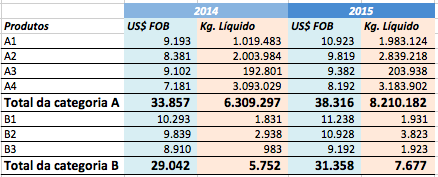
\includegraphics[width=1\linewidth]{imagens/dados_wide} 

}

\caption{Tabela wide}\label{fig:unnamed-chunk-68}
\end{figure}

\begin{figure}

{\centering 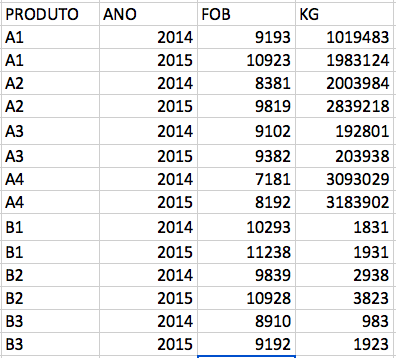
\includegraphics[width=1\linewidth]{imagens/dados_long} 

}

\caption{Tabela long}\label{fig:unnamed-chunk-69}
\end{figure}

A primeira tabela é mais intuitiva para análise visual, pois faz uso de
cores e propõe uma leitura natural, da esquerda para a direita. Ela usa
elementos e estruturas que guiam seus olhos por uma análise de forma
simples. Já a segunda tabela é um pouco árida para se interpretar ``no
olho''.

Há uma ``regra geral'' que diz que um dado bem estruturado deve conter
uma única variável em uma coluna e uma única observação em uma linha.

Observando a primeira tabela com essa regra em mente, podemos perceber
que as observações de ano estão organizadas em colunas. Apesar de estar
num formato ideal para análise visual, esse formato vai dificultar
bastante certas análises sistemáticas. O melhor a se fazer é converter a
primeira tabela para um modelo mais próximo possível da segunda tabela.

Infelizmente não temos como apresentar um passo a passo padrão para
limpeza de dados, pois isso vai depender completamente do tipo de dado
que você receber, da análise que você quer fazer e da sua criatividade
em manipulação de dados. Mas conhecer os pacotes certos ajuda muito
nessa tarefa.

Lembre-se: é muito mais fácil trabalhar no R com dados ``bem
estruturados''``, onde \textbf{\emph{cada coluna deve ser uma única
variável}} e \textbf{\emph{cada linha deve ser uma única observação}}.

Na contramão da limpeza de dados, você provavelmente terá o problema
contrário no final da sua análise. Supondo que você organizou seus dados
perfeitamente, conseguiu executar os modelos que gostaria, gerou
diversos gráficos interessantes e está satisfeito com o resultado. Você
ainda precisará entregar relatórios finais da sua análise em forma de
tabelas sumarizadas e explicativas, de modo que os interessados possam
entender facilmente apenas com uma rápida análise visual. Nesse caso,
que tipo de tabela seria melhor produzir? Provavelmente quem for ler
seus relatórios entenderá mais rapidamente as tabelas mais próximas do
primeiro exemplo mostrado.

É importante aprender a estruturar e desestruturar tabelas de todas as
formas possíveis.

Para ilustrar, veja algumas tabelas disponíveis no pacote
\texttt{tidyverse} ilustrando os diferentes tipos de organização nos
formatos wide e long. Todas as tabelas possuem os mesmos dados e
informações:

\begin{Shaded}
\begin{Highlighting}[]
\KeywordTok{library}\NormalTok{(tidyverse)}
\end{Highlighting}
\end{Shaded}

\begin{Shaded}
\begin{Highlighting}[]
\NormalTok{table1}
\end{Highlighting}
\end{Shaded}

\begin{verbatim}
## # A tibble: 6 x 4
##       country  year  cases population
##         <chr> <int>  <int>      <int>
## 1 Afghanistan  1999    745   19987071
## 2 Afghanistan  2000   2666   20595360
## 3      Brazil  1999  37737  172006362
## 4      Brazil  2000  80488  174504898
## 5       China  1999 212258 1272915272
## 6       China  2000 213766 1280428583
\end{verbatim}

\begin{Shaded}
\begin{Highlighting}[]
\NormalTok{table2}
\end{Highlighting}
\end{Shaded}

\begin{verbatim}
## # A tibble: 12 x 4
##        country  year       type      count
##          <chr> <int>      <chr>      <int>
##  1 Afghanistan  1999      cases        745
##  2 Afghanistan  1999 population   19987071
##  3 Afghanistan  2000      cases       2666
##  4 Afghanistan  2000 population   20595360
##  5      Brazil  1999      cases      37737
##  6      Brazil  1999 population  172006362
##  7      Brazil  2000      cases      80488
##  8      Brazil  2000 population  174504898
##  9       China  1999      cases     212258
## 10       China  1999 population 1272915272
## 11       China  2000      cases     213766
## 12       China  2000 population 1280428583
\end{verbatim}

\begin{Shaded}
\begin{Highlighting}[]
\NormalTok{table3}
\end{Highlighting}
\end{Shaded}

\begin{verbatim}
## # A tibble: 6 x 3
##       country  year              rate
## *       <chr> <int>             <chr>
## 1 Afghanistan  1999      745/19987071
## 2 Afghanistan  2000     2666/20595360
## 3      Brazil  1999   37737/172006362
## 4      Brazil  2000   80488/174504898
## 5       China  1999 212258/1272915272
## 6       China  2000 213766/1280428583
\end{verbatim}

\begin{Shaded}
\begin{Highlighting}[]
\NormalTok{table4a}
\end{Highlighting}
\end{Shaded}

\begin{verbatim}
## # A tibble: 3 x 3
##       country `1999` `2000`
## *       <chr>  <int>  <int>
## 1 Afghanistan    745   2666
## 2      Brazil  37737  80488
## 3       China 212258 213766
\end{verbatim}

\begin{Shaded}
\begin{Highlighting}[]
\NormalTok{table4b}
\end{Highlighting}
\end{Shaded}

\begin{verbatim}
## # A tibble: 3 x 3
##       country     `1999`     `2000`
## *       <chr>      <int>      <int>
## 1 Afghanistan   19987071   20595360
## 2      Brazil  172006362  174504898
## 3       China 1272915272 1280428583
\end{verbatim}

\begin{Shaded}
\begin{Highlighting}[]
\NormalTok{table5}
\end{Highlighting}
\end{Shaded}

\begin{verbatim}
## # A tibble: 6 x 4
##       country century  year              rate
## *       <chr>   <chr> <chr>             <chr>
## 1 Afghanistan      19    99      745/19987071
## 2 Afghanistan      20    00     2666/20595360
## 3      Brazil      19    99   37737/172006362
## 4      Brazil      20    00   80488/174504898
## 5       China      19    99 212258/1272915272
## 6       China      20    00 213766/1280428583
\end{verbatim}

\section{Pacote tidyr}\label{pacote-tidyr}

Apesar das diversas possibilidades de situações que necessitem de
limpeza de dados, a conjugação de 3 pacotes consegue resolver a grande
maioria dos casos: \texttt{dplyr}, \texttt{tidyr}, \texttt{stringr}.

O pacote \texttt{tidyr} é mais um dos pacotes criados pelo Hadley. Esse
fato por si só já traz algumas vantagens: ele se integra perfeitamente
com o \texttt{dplyr} usando o conector \texttt{\%\textgreater{}\%} e tem
a sintaxe de suas funções bastante intuitiva.

\begin{Shaded}
\begin{Highlighting}[]
\KeywordTok{install.packages}\NormalTok{(}\StringTok{"tidyr"}\NormalTok{)}
\KeywordTok{library}\NormalTok{(tidyr)}
\NormalTok{?tidyr}
\end{Highlighting}
\end{Shaded}

O \texttt{tidyr} também tem suas funções organizadas em pequenos
verbetes, onde cada um representa uma tarefa para organizar os dados. Os
verbetes básicos que abordaremos serão os seguintes:

\begin{itemize}
\tightlist
\item
  gather()
\item
  separate()
\item
  spread()
\item
  unite()
\end{itemize}

Vale lembrar que tudo que for feito usando o \texttt{tidyr} é possível
de ser feito também usando o R base, mas e uma forma um pouco menos
intuitiva. Caso queira entender como usar o R base pra isso, procure
mais sobre as funções \texttt{melt()} e \texttt{cast()}

\begin{figure}

{\centering 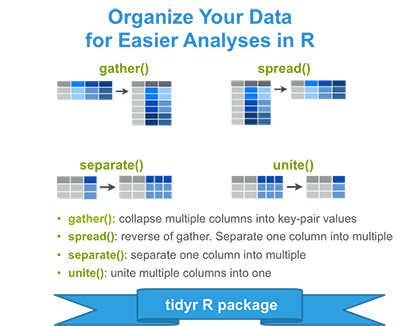
\includegraphics[width=1\linewidth]{imagens/tidyr} 

}

\caption{Tabela long}\label{fig:unnamed-chunk-79}
\end{figure}

\subsection{Gather}\label{gather}

A função \texttt{gather()} serve para agrupar duas ou mais colunas e
seus respectivos valores (conteúdos) em pares de valores. Assim, o
resultado após o agrupamento são sempre duas colunas. A primeira delas
possui observações cujos valores chave eram as colunas antigas e a
segunda, possui os valores respectivos relacionados com as colunas
antigas. Na prática, a função gather diminui o número de colunas e
aumenta o número de linhas de nossa base de dados.

Usaremos dados disponíveis no R base para exemplificar:

\begin{Shaded}
\begin{Highlighting}[]
\KeywordTok{data}\NormalTok{(}\StringTok{"USArrests"}\NormalTok{)}

\KeywordTok{str}\NormalTok{(USArrests)}
\end{Highlighting}
\end{Shaded}

\begin{verbatim}
## 'data.frame':    50 obs. of  4 variables:
##  $ Murder  : num  13.2 10 8.1 8.8 9 7.9 3.3 5.9 15.4 17.4 ...
##  $ Assault : int  236 263 294 190 276 204 110 238 335 211 ...
##  $ UrbanPop: int  58 48 80 50 91 78 77 72 80 60 ...
##  $ Rape    : num  21.2 44.5 31 19.5 40.6 38.7 11.1 15.8 31.9 25.8 ...
\end{verbatim}

\begin{Shaded}
\begin{Highlighting}[]
\KeywordTok{head}\NormalTok{(USArrests)}
\end{Highlighting}
\end{Shaded}

\begin{verbatim}
##            Murder Assault UrbanPop Rape
## Alabama      13.2     236       58 21.2
## Alaska       10.0     263       48 44.5
## Arizona       8.1     294       80 31.0
## Arkansas      8.8     190       50 19.5
## California    9.0     276       91 40.6
## Colorado      7.9     204       78 38.7
\end{verbatim}

\begin{Shaded}
\begin{Highlighting}[]
\CommentTok{# Transformando o nome das linhas em colunas}
\NormalTok{USArrests}\OperatorTok{$}\NormalTok{State <-}\StringTok{ }\KeywordTok{rownames}\NormalTok{(USArrests)}
\KeywordTok{head}\NormalTok{(USArrests)}
\end{Highlighting}
\end{Shaded}

\begin{verbatim}
##            Murder Assault UrbanPop Rape      State
## Alabama      13.2     236       58 21.2    Alabama
## Alaska       10.0     263       48 44.5     Alaska
## Arizona       8.1     294       80 31.0    Arizona
## Arkansas      8.8     190       50 19.5   Arkansas
## California    9.0     276       91 40.6 California
## Colorado      7.9     204       78 38.7   Colorado
\end{verbatim}

\begin{Shaded}
\begin{Highlighting}[]
\NormalTok{usa.long <-}\StringTok{ }\NormalTok{USArrests }\OperatorTok\StringTok{ }
\StringTok{  }\KeywordTok{gather}\NormalTok{(}\DataTypeTok{key =} \StringTok{"tipo_crime"}\NormalTok{, }\DataTypeTok{value =} \StringTok{"valor"}\NormalTok{, }\OperatorTok{-}\NormalTok{State)}

\KeywordTok{head}\NormalTok{(usa.long)}
\end{Highlighting}
\end{Shaded}

\begin{verbatim}
##        State tipo_crime valor
## 1    Alabama     Murder  13.2
## 2     Alaska     Murder  10.0
## 3    Arizona     Murder   8.1
## 4   Arkansas     Murder   8.8
## 5 California     Murder   9.0
## 6   Colorado     Murder   7.9
\end{verbatim}

\begin{Shaded}
\begin{Highlighting}[]
\KeywordTok{tail}\NormalTok{(usa.long)}
\end{Highlighting}
\end{Shaded}

\begin{verbatim}
##             State tipo_crime valor
## 195       Vermont       Rape  11.2
## 196      Virginia       Rape  20.7
## 197    Washington       Rape  26.2
## 198 West Virginia       Rape   9.3
## 199     Wisconsin       Rape  10.8
## 200       Wyoming       Rape  15.6
\end{verbatim}

No primeiro parâmetro do \texttt{gather()} nós informamos a ``chave'',
ou seja, a coluna que guardará o que antes era coluna. No segundo
parâmetro informamos o ``value'', ou seja, a coluna que guardar os
valores para cada uma das antigas colunas. Reparem que agora você pode
afirmar com certeza que cada linha é uma observação e que cada coluna é
uma variável.

\subsection{Spread}\label{spread}

É a operação antagônica do \texttt{gather()}. Ela espalha os valores de
duas colunas em diversos campos para cada registro: os valores de uma
coluna viram o nome das novas colunas, e os valores de outra virão
valores de cada registro nas novas colunas. Usaremos a \texttt{table2}
para exemplificar:

\begin{Shaded}
\begin{Highlighting}[]
\KeywordTok{head}\NormalTok{(table2)}
\end{Highlighting}
\end{Shaded}

\begin{verbatim}
## # A tibble: 6 x 4
##       country  year       type     count
##         <chr> <int>      <chr>     <int>
## 1 Afghanistan  1999      cases       745
## 2 Afghanistan  1999 population  19987071
## 3 Afghanistan  2000      cases      2666
## 4 Afghanistan  2000 population  20595360
## 5      Brazil  1999      cases     37737
## 6      Brazil  1999 population 172006362
\end{verbatim}

\begin{Shaded}
\begin{Highlighting}[]
\NormalTok{table2.wide <-}\StringTok{ }\NormalTok{table2 }\OperatorTok
\StringTok{  }\KeywordTok{spread}\NormalTok{(}\DataTypeTok{key =}\NormalTok{ type, }\DataTypeTok{value =}\NormalTok{ count)}

\KeywordTok{head}\NormalTok{(table2.wide)}
\end{Highlighting}
\end{Shaded}

\begin{verbatim}
## # A tibble: 6 x 4
##       country  year  cases population
##         <chr> <int>  <int>      <int>
## 1 Afghanistan  1999    745   19987071
## 2 Afghanistan  2000   2666   20595360
## 3      Brazil  1999  37737  172006362
## 4      Brazil  2000  80488  174504898
## 5       China  1999 212258 1272915272
## 6       China  2000 213766 1280428583
\end{verbatim}

\subsection{Separate}\label{separate}

O \texttt{separate()} é usado para separar duas variáveis que estão em
uma mesma coluna. Lembr-se: ``cada coluna deve ser apenas uma única
variável''. É muito normal virem variáveis juntas em uma única coluna,
mas nem sempre isso é prejudicial, cabe avaliar quando vale a pena
separar.

Usaremos o exemplo da \texttt{table3} para investigar:

\begin{Shaded}
\begin{Highlighting}[]
\NormalTok{table3.wide <-}\StringTok{ }\NormalTok{table3 }\OperatorTok\StringTok{ }
\StringTok{  }\KeywordTok{separate}\NormalTok{(rate, }\DataTypeTok{into =} \KeywordTok{c}\NormalTok{(}\StringTok{"cases"}\NormalTok{, }\StringTok{"population"}\NormalTok{), }\DataTypeTok{sep=}\StringTok{'/'}\NormalTok{)}

\KeywordTok{head}\NormalTok{(table3.wide)}
\end{Highlighting}
\end{Shaded}

\begin{verbatim}
## # A tibble: 6 x 4
##       country  year  cases population
##         <chr> <int>  <chr>      <chr>
## 1 Afghanistan  1999    745   19987071
## 2 Afghanistan  2000   2666   20595360
## 3      Brazil  1999  37737  172006362
## 4      Brazil  2000  80488  174504898
## 5       China  1999 212258 1272915272
## 6       China  2000 213766 1280428583
\end{verbatim}

\subsection{Unite}\label{unite}

A operação \texttt{unite()} é o oposto da \texttt{separate()}, ela pega
duas colunas (variáveis) e transforma em uma só. Muito utilizada para
montar relatórios finais ou tabelas para análise visual. Vamos
aproveitar o exemplo em \texttt{table2} e montar uma tabela final
comparando a case e population de cada pais em cada ano.

\begin{Shaded}
\begin{Highlighting}[]
\NormalTok{table2.relatorio <-}\StringTok{ }\NormalTok{table2 }\OperatorTok\StringTok{ }
\StringTok{  }\KeywordTok{unite}\NormalTok{(type_year, type, year) }\OperatorTok\StringTok{ }
\StringTok{  }\KeywordTok{spread}\NormalTok{(}\DataTypeTok{key =}\NormalTok{ type_year, }\DataTypeTok{value =}\NormalTok{ count, }\DataTypeTok{sep =} \StringTok{'_'}\NormalTok{)}
  
\NormalTok{table2.relatorio}
\end{Highlighting}
\end{Shaded}

\begin{verbatim}
## # A tibble: 3 x 5
##       country type_year_cases_1999 type_year_cases_2000
## *       <chr>                <int>                <int>
## 1 Afghanistan                  745                 2666
## 2      Brazil                37737                80488
## 3       China               212258               213766
## # ... with 2 more variables: type_year_population_1999 <int>,
## #   type_year_population_2000 <int>
\end{verbatim}

O primeiro parâmetro é a coluna que desejamos criar, os próximos são as
colunas que desejamos unir e por fim temos o \texttt{sep}, que é algum
símbolo opcional para ficar entre os dois valores na nova coluna.

\section{Manipulação de texto}\label{manipulacao-de-texto}

Manipulação de texto também é algo importante em ciência de dados, pois
nem tudo são números, existem variáveis categóricas que são baseadas em
texto. Mais uma vez, esse tipo de manipulação depende do tipo de arquivo
que você receber.

\begin{Shaded}
\begin{Highlighting}[]
\NormalTok{a <-}\StringTok{ 'texto 1'}
\NormalTok{b <-}\StringTok{ 'texto 2'}
\NormalTok{c <-}\StringTok{ 'texto 3'}
\KeywordTok{paste}\NormalTok{(a, b, c)}
\end{Highlighting}
\end{Shaded}

\begin{verbatim}
## [1] "texto 1 texto 2 texto 3"
\end{verbatim}

O \texttt{paste()} é a função mais básica para manipulação de textos
usando o R base. Ela simplesmente concatena todas as variáveis textuais
que você informar. Existe um parâmetro, extra (\texttt{sep}) cujo valor
padrão é espaço ` `.

\begin{Shaded}
\begin{Highlighting}[]
\KeywordTok{paste}\NormalTok{(a, b, c, }\DataTypeTok{sep =} \StringTok{'-'}\NormalTok{)}
\end{Highlighting}
\end{Shaded}

\begin{verbatim}
## [1] "texto 1-texto 2-texto 3"
\end{verbatim}

\begin{Shaded}
\begin{Highlighting}[]
\KeywordTok{paste}\NormalTok{(a, b, c, }\DataTypeTok{sep =} \StringTok{';'}\NormalTok{)}
\end{Highlighting}
\end{Shaded}

\begin{verbatim}
## [1] "texto 1;texto 2;texto 3"
\end{verbatim}

\begin{Shaded}
\begin{Highlighting}[]
\KeywordTok{paste}\NormalTok{(a, b, c, }\DataTypeTok{sep =} \StringTok{'---%---'}\NormalTok{)}
\end{Highlighting}
\end{Shaded}

\begin{verbatim}
## [1] "texto 1---%---texto 2---%---texto 3"
\end{verbatim}

\subsection{Pacote stringr}\label{pacote-stringr}

Texto no R é sempre do tipo \texttt{character}. No universo da
computação, também se referem a texto como \texttt{string}. E é daí que
vem o nome desse pacote, também criado por Hadley Wickham. Por um acaso
esse pacote não está incluído no pacote \texttt{tidyverse}.

\begin{Shaded}
\begin{Highlighting}[]
\KeywordTok{install.packages}\NormalTok{(}\StringTok{'stringr'}\NormalTok{)}
\KeywordTok{library}\NormalTok{(stringr)}
\NormalTok{?stringr}
\end{Highlighting}
\end{Shaded}

Começaremos pela função \texttt{str\_sub()}, que extrai apenas parte de
um texto.

\begin{Shaded}
\begin{Highlighting}[]
\NormalTok{cnae.texto <-}\StringTok{ }\KeywordTok{c}\NormalTok{(}\StringTok{'10 Fabricação de produtos alimentícios'}\NormalTok{, }\StringTok{'11 Fabricação de bebidas'}\NormalTok{, }
             \StringTok{'12 Fabricação de produtos do fumo'}\NormalTok{, }\StringTok{'13 Fabricação de produtos têxteis', }
\StringTok{             '}\DecValTok{14}\NormalTok{ Confecção de artigos do vestuário e acessórios',}
             \StringTok{'15 Preparação de couros e fabricação de artefatos de couro, artigos para viagem e calçados'}\NormalTok{,}
             \StringTok{'16 Fabricação de produtos de madeira'}\NormalTok{, }
             \StringTok{'17 Fabricação de celulose, papel e produtos de papel'}\NormalTok{)}
\NormalTok{cnae <-}\StringTok{ }\KeywordTok{str_sub}\NormalTok{(cnae.texto, }\DecValTok{0}\NormalTok{, }\DecValTok{2}\NormalTok{)}
\NormalTok{texto <-}\StringTok{ }\KeywordTok{str_sub}\NormalTok{(cnae.texto, }\DecValTok{4}\NormalTok{)}

\NormalTok{cnae}
\end{Highlighting}
\end{Shaded}

\begin{verbatim}
## [1] "10" "11" "12" "13" "14" "15" "16" "17"
\end{verbatim}

\begin{Shaded}
\begin{Highlighting}[]
\NormalTok{texto}
\end{Highlighting}
\end{Shaded}

\begin{verbatim}
## [1] "Fabricação de produtos alimentícios"                                                    
## [2] "Fabricação de bebidas"                                                                  
## [3] "Fabricação de produtos do fumo"                                                         
## [4] "Fabricação de produtos têxteis"                                                         
## [5] "Confecção de artigos do vestuário e acessórios"                                         
## [6] "Preparação de couros e fabricação de artefatos de couro, artigos para viagem e calçados"
## [7] "Fabricação de produtos de madeira"                                                      
## [8] "Fabricação de celulose, papel e produtos de papel"
\end{verbatim}

Temos também a função \texttt{str\_replace()} e
\texttt{str\_replace\_all()}, que substitui determinados caracteres por
outros. Tal como no exemplo a seguir:

\begin{Shaded}
\begin{Highlighting}[]
\NormalTok{telefones <-}\StringTok{ }\KeywordTok{c}\NormalTok{(}\StringTok{'9931-9512'}\NormalTok{, }\StringTok{'8591-5892'}\NormalTok{, }\StringTok{'8562-1923'}\NormalTok{)}
\KeywordTok{str_replace}\NormalTok{(telefones, }\StringTok{'-'}\NormalTok{, }\StringTok{''}\NormalTok{)}
\end{Highlighting}
\end{Shaded}

\begin{verbatim}
## [1] "99319512" "85915892" "85621923"
\end{verbatim}

\begin{Shaded}
\begin{Highlighting}[]
\NormalTok{cnpj <-}\StringTok{ }\KeywordTok{c}\NormalTok{(}\StringTok{'19.702.231/9999-98'}\NormalTok{, }\StringTok{'19.498.482/9999-05'}\NormalTok{, }\StringTok{'19.499.583/9999-50'}\NormalTok{, }\StringTok{'19.500.999/9999-46'}\NormalTok{, }\StringTok{'19.501.139/9999-90'}\NormalTok{)}
\KeywordTok{str_replace_all}\NormalTok{(cnpj, }\StringTok{'}\CharTok{\textbackslash{}\textbackslash{}}\StringTok{.|/|-'}\NormalTok{, }\StringTok{''}\NormalTok{)}
\end{Highlighting}
\end{Shaded}

\begin{verbatim}
## [1] "19702231999998" "19498482999905" "19499583999950" "19500999999946"
## [5] "19501139999990"
\end{verbatim}

O que são esses símbolos no segundo exemplo? São símbolos especiais
utilizados em funções textuais para reconhecimento de padrão. Esses
símbolos são conhecidos como \textbf{Expressões Regulares} ou o famoso
\textbf{Regex}.

\subsection{Regex}\label{regex}

Trata-se de um assunto bastante complexo e avançado. Não é fácil dominar
regex e provavelmente você vai precisar sempre consultar e exprimentar a
montagem dos padrões de regex. Infelizmente não é possível aprender
regex rápido e de um jeito fácil, só existe o jeito difícil: errando
muito, e com muita prática e experiências reais.

A seguir, uma lista dos principais mecanimos de regex:

\begin{longtable}[]{@{}cr@{}}
\toprule
regex & correspondência\tabularnewline
\midrule
\endhead
\texttt{\^{}} & começa do string (ou uma negação)\tabularnewline
\texttt{.} & qualquer caracter\tabularnewline
\texttt{\$} & fim da linha\tabularnewline
\texttt{{[}maça{]}} & procura as caracteres \texttt{m}, \texttt{a},
\texttt{ç}\tabularnewline
\texttt{maça} & \texttt{maça}\tabularnewline
\texttt{{[}0-9{]}} & números\tabularnewline
\texttt{{[}A-Z{]}} & qualquer letra maiúscula\tabularnewline
\texttt{\textbackslash{}\textbackslash{}w} & uma palavra\tabularnewline
\texttt{\textbackslash{}\textbackslash{}W} & não é
palavra\tabularnewline
& (é puntuação, espaço etc.)\tabularnewline
\texttt{\textbackslash{}\textbackslash{}s} & um espaço (tab, newline,
space)\tabularnewline
\bottomrule
\end{longtable}

A seguir, alguns bons sites para aprender mais sobre regex. É um assunto
interessante e bastante utilizado para tratamento textual.

\url{http://turing.com.br/material/regex/introducao.html}

\url{https://regexone.com/}

\section{Exercícios}\label{exercicios-4}

\begin{enumerate}
\def\labelenumi{\arabic{enumi}.}
\tightlist
\item
  Utilizando senado.csv monte uma tabela mostrando a quantidade de votos
  sim e não por coalisão, no formato wide (sim e não são linhas e
  coalisão ou não coalisão são colunas)
  \texttt{Dica:\ mutate(tipo\_coalisao\ =\ ifelse(GovCoalition,\ \textquotesingle{}Coalisão\textquotesingle{},\ \textquotesingle{}Não\ Coalisão\textquotesingle{}))}
\end{enumerate}

\begin{verbatim}
## # A tibble: 2 x 3
##   Tipo_voto Coalisão `Não Coalisão`
##       <chr>    <int>          <int>
## 1 Votos Não      702            657
## 2 Votos Sim     5002           2739
\end{verbatim}

\begin{enumerate}
\def\labelenumi{\arabic{enumi}.}
\setcounter{enumi}{1}
\tightlist
\item
  Utilizando o dataframe abaixo, obtenha o resultado a seguinte.
  \texttt{Dica:\ separate(),\ str\_replace\_all(),\ str\_trim(),\ str\_sub()}
\end{enumerate}

\begin{Shaded}
\begin{Highlighting}[]
\NormalTok{cadastros <-}\StringTok{ }\KeywordTok{data.frame}\NormalTok{(}
  \DataTypeTok{email =} \KeywordTok{c}\NormalTok{(}\StringTok{'joaodasilva@gmail.com'}\NormalTok{, }\StringTok{'rafael@hotmail.com'}\NormalTok{, }\StringTok{'maria@uol.com.br'}\NormalTok{, }\StringTok{'juliana.morais@outlook.com'}\NormalTok{),}
  \DataTypeTok{telefone =} \KeywordTok{c}\NormalTok{(}\StringTok{'(61)99831-9482'}\NormalTok{, }\StringTok{'32 8976 2913'}\NormalTok{, }\StringTok{'62-9661-1234'}\NormalTok{, }\StringTok{'15-40192.5812'}\NormalTok{)}
\NormalTok{)}

\NormalTok{cadastros}
\end{Highlighting}
\end{Shaded}

\begin{verbatim}
##                        email       telefone
## 1      joaodasilva@gmail.com (61)99831-9482
## 2         rafael@hotmail.com   32 8976 2913
## 3           maria@uol.com.br   62-9661-1234
## 4 juliana.morais@outlook.com  15-40192.5812
\end{verbatim}

\begin{verbatim}
##            login dominio   telefone dd
## 1    joaodasilva   gmail 99831-9482 61
## 2         rafael hotmail  8976-2913 32
## 3          maria     uol  9661-1234 62
## 4 juliana.morais outlook 40192-5812 15
\end{verbatim}

\chapter{Juntando dados}\label{juntando-dados}

Existem duas grandes formas de junção de dados: \textbf{UNIÃO} e
\textbf{CRUZAMENTO}.

Para que uma união seja possível, os dois conjuntos de dados precisam
ter os mesmos campos. Para que um cruzamento seja possível, os dois
conjuntos precisam ter pelo menos um campo em comum.

\begin{figure}

{\centering 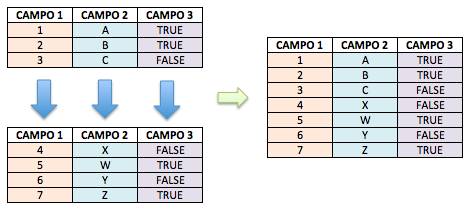
\includegraphics[width=1\linewidth]{imagens/union} 

}

\caption{União de tabelas}\label{fig:unnamed-chunk-96}
\end{figure}

\begin{figure}

{\centering 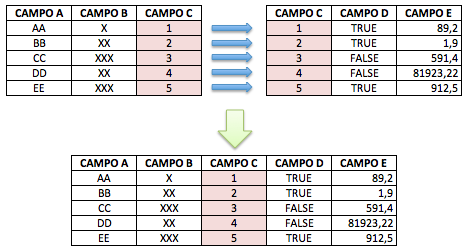
\includegraphics[width=1\linewidth]{imagens/join} 

}

\caption{Cruzamento de tabelas}\label{fig:unnamed-chunk-97}
\end{figure}

\section{União de dados (Union)}\label{uniao-de-dados-union}

A união de dados é mais intuitiva. Basta ter a mesma quantidade de
campos e que os campos estejam ``alinhados''. A função mais usada para
isso é o famoso \texttt{rbind()} (Row Bind). Caso os campos tenham
exatamente os mesmos nomes e tipo, o \texttt{rbind()} consegue fazer a
união perfeitamente.

\begin{Shaded}
\begin{Highlighting}[]
\NormalTok{dados2016 <-}\StringTok{ }\KeywordTok{data.frame}\NormalTok{(}\DataTypeTok{ano =} \KeywordTok{c}\NormalTok{(}\DecValTok{2016}\NormalTok{, }\DecValTok{2016}\NormalTok{, }\DecValTok{2016}\NormalTok{), }
                        \DataTypeTok{valor =} \KeywordTok{c}\NormalTok{(}\DecValTok{938}\NormalTok{, }\DecValTok{113}\NormalTok{, }\DecValTok{1748}\NormalTok{), }
                        \DataTypeTok{produto =} \KeywordTok{c}\NormalTok{(}\StringTok{'A'}\NormalTok{, }\StringTok{'B'}\NormalTok{, }\StringTok{'C'}\NormalTok{))}

\NormalTok{dados2017 <-}\StringTok{ }\KeywordTok{data.frame}\NormalTok{(}\DataTypeTok{valor =} \KeywordTok{c}\NormalTok{(}\DecValTok{8400}\NormalTok{, }\DecValTok{837}\NormalTok{, }\DecValTok{10983}\NormalTok{), }
                        \DataTypeTok{produto =} \KeywordTok{c}\NormalTok{(}\StringTok{'H'}\NormalTok{, }\StringTok{'Z'}\NormalTok{, }\StringTok{'X'}\NormalTok{),}
                        \DataTypeTok{ano =} \KeywordTok{c}\NormalTok{(}\DecValTok{2017}\NormalTok{, }\DecValTok{2017}\NormalTok{, }\DecValTok{2017}\NormalTok{))}

\NormalTok{dados.finais <-}\StringTok{ }\KeywordTok{rbind}\NormalTok{(dados2016, dados2017)}

\NormalTok{dados.finais}
\end{Highlighting}
\end{Shaded}

\begin{verbatim}
##    ano valor produto
## 1 2016   938       A
## 2 2016   113       B
## 3 2016  1748       C
## 4 2017  8400       H
## 5 2017   837       Z
## 6 2017 10983       X
\end{verbatim}

União de dados é a forma mais simples de juntar dados.

\section{Cruzamento de Dados (Join)}\label{cruzamento-de-dados-join}

O cruzamento de dados é um pouco mais complexo, mas nem por isso chega a
ser algo difícil.

Para entender como fazer joins (cruzamentos) é preciso entender o
conceito de \textbf{chave}. Entenda chave como uma coluna que está
presente da mesma forma em dois conjuntos de dados distintos. O conceito
completo de chave é bem mais complexo que isso, mas para começar a
entender e usar os joins, basta usar essa intuição.

Tendo o conceito de chave em mente, a primeira coisa que deve fazer
quando precisar cruzar dois conjuntos de dados é tentar identificar
quais os campos chaves, ou seja, quais os campos estão presentes nos
dois grupos.

O que acontece quando nem todos os códigos de um grupo esão no outro? E
quando um grupo tem códigos repetidos em várias linhas? Para responder
essas e outras perguntas precisamos conhecer os diferentes tipos de
joins. Existe pelo menos uma dezena de tipos de joins, mas 90\% das
vezes você precisará apenas dos tipos básicos que explicaremos a seguir.
Usaremos o pacote \texttt{dplyr} para aplicar os joins. O R base possui
a função \texttt{merge()} para joins, se tiver curiosidade procure mais
sobre ela depois.

\subsection{Inner Join (ou apenas
Join)}\label{inner-join-ou-apenas-join}

Trata-se do join mais simples, mais básico e mais usado dentre todos os
outros tipos. O seu comportamento mantem no resultado apenas as linhas
que estão presente nos dois conjuntos de dados que estão sendo cruzados.
O inner join funciona da seguinte forma:

\begin{figure}

{\centering 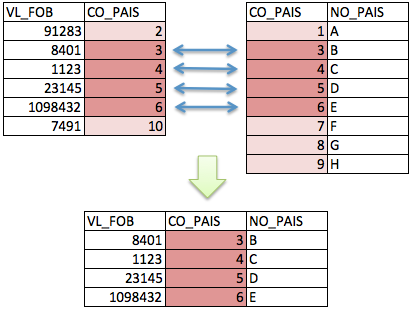
\includegraphics[width=1\linewidth]{imagens/inner_join} 

}

\caption{Cruzamento de tabelas}\label{fig:unnamed-chunk-99}
\end{figure}

A tabela final após o cruzamento conterá as linhas com as chaves que
estiverem em AMBOS os conjuntos de dados. As linhas com chaves que não
estão em ambos serão descartadas. Essa característica torna o inner join
muito útil para fazer filtros.

Vamos utilizar dados já disponíveis no \texttt{dplyr} para testar os
joins:

\begin{Shaded}
\begin{Highlighting}[]
\NormalTok{band_members}
\end{Highlighting}
\end{Shaded}

\begin{verbatim}
## # A tibble: 3 x 2
##    name    band
##   <chr>   <chr>
## 1  Mick  Stones
## 2  John Beatles
## 3  Paul Beatles
\end{verbatim}

\begin{Shaded}
\begin{Highlighting}[]
\NormalTok{band_instruments}
\end{Highlighting}
\end{Shaded}

\begin{verbatim}
## # A tibble: 3 x 2
##    name  plays
##   <chr>  <chr>
## 1  John guitar
## 2  Paul   bass
## 3 Keith guitar
\end{verbatim}

\begin{Shaded}
\begin{Highlighting}[]
\KeywordTok{str}\NormalTok{(band_members)}
\end{Highlighting}
\end{Shaded}

\begin{verbatim}
## Classes 'tbl_df', 'tbl' and 'data.frame':    3 obs. of  2 variables:
##  $ name: chr  "Mick" "John" "Paul"
##  $ band: chr  "Stones" "Beatles" "Beatles"
\end{verbatim}

\begin{Shaded}
\begin{Highlighting}[]
\KeywordTok{str}\NormalTok{(band_instruments)}
\end{Highlighting}
\end{Shaded}

\begin{verbatim}
## Classes 'tbl_df', 'tbl' and 'data.frame':    3 obs. of  2 variables:
##  $ name : chr  "John" "Paul" "Keith"
##  $ plays: chr  "guitar" "bass" "guitar"
\end{verbatim}

\begin{Shaded}
\begin{Highlighting}[]
\CommentTok{#vamos juntar os dois conjuntos com um join}

\NormalTok{band_members }\OperatorTok\StringTok{ }\KeywordTok{inner_join}\NormalTok{(band_instruments) }
\end{Highlighting}
\end{Shaded}

\begin{verbatim}
## # A tibble: 2 x 3
##    name    band  plays
##   <chr>   <chr>  <chr>
## 1  John Beatles guitar
## 2  Paul Beatles   bass
\end{verbatim}

\begin{Shaded}
\begin{Highlighting}[]
\CommentTok{#o dplyr "adivinhou" a coluna chave pelo nome}
\end{Highlighting}
\end{Shaded}

Repare que nesse caso a chave é a coluna \texttt{name}. Repare também
que os dois conjuntos tem 3 registros. Então por que o resultado final
só tem 2 registros? Pois o comportamento do join é justamente retornar
apenas as linhas em que as chaves coincidiram (efeito de filtro).

Vamos fazer o mesmo experimento com \texttt{band\_intruments2}

\begin{Shaded}
\begin{Highlighting}[]
\NormalTok{band_instruments2}
\end{Highlighting}
\end{Shaded}

\begin{verbatim}
## # A tibble: 3 x 2
##   artist  plays
##    <chr>  <chr>
## 1   John guitar
## 2   Paul   bass
## 3  Keith guitar
\end{verbatim}

\begin{Shaded}
\begin{Highlighting}[]
\KeywordTok{str}\NormalTok{(band_instruments2) }\CommentTok{#o nome da coluna é diferente}
\end{Highlighting}
\end{Shaded}

\begin{verbatim}
## Classes 'tbl_df', 'tbl' and 'data.frame':    3 obs. of  2 variables:
##  $ artist: chr  "John" "Paul" "Keith"
##  $ plays : chr  "guitar" "bass" "guitar"
\end{verbatim}

\begin{Shaded}
\begin{Highlighting}[]
\NormalTok{band_members }\OperatorTok\StringTok{ }\KeywordTok{inner_join}\NormalTok{(band_instruments2, }\DataTypeTok{by =} \KeywordTok{c}\NormalTok{(}\StringTok{'name'}\NormalTok{ =}\StringTok{ 'artist'}\NormalTok{))}
\end{Highlighting}
\end{Shaded}

\begin{verbatim}
## # A tibble: 2 x 3
##    name    band  plays
##   <chr>   <chr>  <chr>
## 1  John Beatles guitar
## 2  Paul Beatles   bass
\end{verbatim}

Repare que dessa vez tivemos que especificar qual a coluna chave para
que o join aconteça.

Mais um exemplo:

\begin{Shaded}
\begin{Highlighting}[]
\KeywordTok{setwd}\NormalTok{(}\StringTok{'dados'}\NormalTok{)}
\end{Highlighting}
\end{Shaded}

\begin{Shaded}
\begin{Highlighting}[]
\NormalTok{empregados <-}\StringTok{ }\KeywordTok{read_csv}\NormalTok{(}\StringTok{'dados/Employees.csv'}\NormalTok{)}
\NormalTok{departamentos <-}\StringTok{ }\KeywordTok{read_csv}\NormalTok{(}\StringTok{'dados/Departments.csv'}\NormalTok{)}

\KeywordTok{str}\NormalTok{(empregados)}
\end{Highlighting}
\end{Shaded}

\begin{verbatim}
## Classes 'tbl_df', 'tbl' and 'data.frame':    6 obs. of  4 variables:
##  $ Employee    : int  1 2 3 4 5 6
##  $ EmployeeName: chr  "Alice" "Bob" "Carla" "Daniel" ...
##  $ Department  : int  11 11 12 12 13 21
##  $ Salary      : int  800 600 900 1000 800 700
##  - attr(*, "spec")=List of 2
##   ..$ cols   :List of 4
##   .. ..$ Employee    : list()
##   .. .. ..- attr(*, "class")= chr  "collector_integer" "collector"
##   .. ..$ EmployeeName: list()
##   .. .. ..- attr(*, "class")= chr  "collector_character" "collector"
##   .. ..$ Department  : list()
##   .. .. ..- attr(*, "class")= chr  "collector_integer" "collector"
##   .. ..$ Salary      : list()
##   .. .. ..- attr(*, "class")= chr  "collector_integer" "collector"
##   ..$ default: list()
##   .. ..- attr(*, "class")= chr  "collector_guess" "collector"
##   ..- attr(*, "class")= chr "col_spec"
\end{verbatim}

\begin{Shaded}
\begin{Highlighting}[]
\KeywordTok{str}\NormalTok{(departamentos)}
\end{Highlighting}
\end{Shaded}

\begin{verbatim}
## Classes 'tbl_df', 'tbl' and 'data.frame':    4 obs. of  3 variables:
##  $ Department    : int  11 12 13 14
##  $ DepartmentName: chr  "Production" "Sales" "Marketing" "Research"
##  $ Manager       : int  1 4 5 NA
##  - attr(*, "spec")=List of 2
##   ..$ cols   :List of 3
##   .. ..$ Department    : list()
##   .. .. ..- attr(*, "class")= chr  "collector_integer" "collector"
##   .. ..$ DepartmentName: list()
##   .. .. ..- attr(*, "class")= chr  "collector_character" "collector"
##   .. ..$ Manager       : list()
##   .. .. ..- attr(*, "class")= chr  "collector_integer" "collector"
##   ..$ default: list()
##   .. ..- attr(*, "class")= chr  "collector_guess" "collector"
##   ..- attr(*, "class")= chr "col_spec"
\end{verbatim}

\begin{Shaded}
\begin{Highlighting}[]
\NormalTok{empregados}
\end{Highlighting}
\end{Shaded}

\begin{verbatim}
## # A tibble: 6 x 4
##   Employee EmployeeName Department Salary
##      <int>        <chr>      <int>  <int>
## 1        1        Alice         11    800
## 2        2          Bob         11    600
## 3        3        Carla         12    900
## 4        4       Daniel         12   1000
## 5        5       Evelyn         13    800
## 6        6    Ferdinand         21    700
\end{verbatim}

\begin{Shaded}
\begin{Highlighting}[]
\NormalTok{departamentos}
\end{Highlighting}
\end{Shaded}

\begin{verbatim}
## # A tibble: 4 x 3
##   Department DepartmentName Manager
##        <int>          <chr>   <int>
## 1         11     Production       1
## 2         12          Sales       4
## 3         13      Marketing       5
## 4         14       Research      NA
\end{verbatim}

\begin{Shaded}
\begin{Highlighting}[]
\NormalTok{final <-}\StringTok{ }\NormalTok{empregados }\OperatorTok\StringTok{ }
\StringTok{  }\KeywordTok{inner_join}\NormalTok{(departamentos, }\DataTypeTok{by =} \KeywordTok{c}\NormalTok{(}\StringTok{'Employee'}\NormalTok{ =}\StringTok{ 'Manager'}\NormalTok{))}

\NormalTok{final}
\end{Highlighting}
\end{Shaded}

\begin{verbatim}
## # A tibble: 3 x 6
##   Employee EmployeeName Department.x Salary Department.y DepartmentName
##      <int>        <chr>        <int>  <int>        <int>          <chr>
## 1        1        Alice           11    800           11     Production
## 2        4       Daniel           12   1000           12          Sales
## 3        5       Evelyn           13    800           13      Marketing
\end{verbatim}

Novamente tivemos o mesmo efeito, listamos apenas os empregados que são
Gerentes de departamento.

Acontece que existem situações em que esse descarte de registro do inner
join não é interessante. Nesses casos usamos outros tipos de join: os
Outer Joins. Existem 3 tipos básicos de outer join: left outer join (ou
só left join), o right outer join (ou só right join) e full outer join
(ou apenas full join)

\subsection{Left Outer Join}\label{left-outer-join}

Chama-se \textbf{LEFT} outer join pois todos os registros do ``conjunto
da esquerda'' estarão presentes no resultado final, além dos registros
da direita que coincidirem na chave. Podemos usar no caso a seguir.

\begin{Shaded}
\begin{Highlighting}[]
\NormalTok{band_members }\OperatorTok\StringTok{ }\KeywordTok{left_join}\NormalTok{(band_instruments2, }\DataTypeTok{by =} \KeywordTok{c}\NormalTok{(}\StringTok{'name'}\NormalTok{ =}\StringTok{ 'artist'}\NormalTok{))}
\end{Highlighting}
\end{Shaded}

\begin{verbatim}
## # A tibble: 3 x 3
##    name    band  plays
##   <chr>   <chr>  <chr>
## 1  Mick  Stones   <NA>
## 2  John Beatles guitar
## 3  Paul Beatles   bass
\end{verbatim}

\begin{Shaded}
\begin{Highlighting}[]
\NormalTok{band_instruments2}
\end{Highlighting}
\end{Shaded}

\begin{verbatim}
## # A tibble: 3 x 2
##   artist  plays
##    <chr>  <chr>
## 1   John guitar
## 2   Paul   bass
## 3  Keith guitar
\end{verbatim}

Reparem no efeito: mesmo Mick não tendo referência no conjunto de dados
``da direita'' (band\_instruments2) ele apareceu no registro final com
\texttt{NA} no campo que diz respeito ao conjunto da direita. Da mesma
forma, Keith não está presente no conjunto final pois não tem referência
no conjunto da esquerda.

\begin{figure}

{\centering 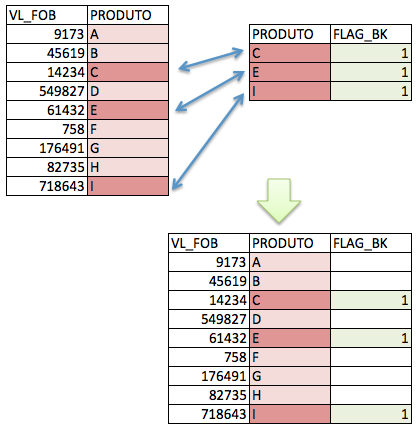
\includegraphics[width=1\linewidth]{imagens/left_join} 

}

\caption{Cruzamento de tabelas}\label{fig:unnamed-chunk-105}
\end{figure}

Repare que a ``posição'' das tabelas faz diferença. No caso da nossa
manipulação de exmeplo, aplicamos o left join pois a tabela que
queríamos preservar estava ``à esquerda'' na manipulação.

\begin{Shaded}
\begin{Highlighting}[]
\NormalTok{final2 <-}\StringTok{ }\NormalTok{empregados }\OperatorTok\StringTok{ }
\StringTok{  }\KeywordTok{left_join}\NormalTok{(departamentos, }\DataTypeTok{by =} \KeywordTok{c}\NormalTok{(}\StringTok{'Employee'}\NormalTok{ =}\StringTok{ 'Manager'}\NormalTok{))}

\NormalTok{final2}
\end{Highlighting}
\end{Shaded}

\begin{verbatim}
## # A tibble: 6 x 6
##   Employee EmployeeName Department.x Salary Department.y DepartmentName
##      <int>        <chr>        <int>  <int>        <int>          <chr>
## 1        1        Alice           11    800           11     Production
## 2        2          Bob           11    600           NA           <NA>
## 3        3        Carla           12    900           NA           <NA>
## 4        4       Daniel           12   1000           12          Sales
## 5        5       Evelyn           13    800           13      Marketing
## 6        6    Ferdinand           21    700           NA           <NA>
\end{verbatim}

\subsection{Right Outer Join}\label{right-outer-join}

O princípio é EXATAMENTE o mesmo do left join. A única diferença é a
permanência dos registros do conjunto da direita. Podemos chegar ao
mesmo resultado anterior apenas mudando os data frames de posição na
manipulação.

\begin{Shaded}
\begin{Highlighting}[]
\NormalTok{final3 <-}\StringTok{ }\NormalTok{departamentos }\OperatorTok\StringTok{ }
\StringTok{  }\KeywordTok{right_join}\NormalTok{(empregados, }\DataTypeTok{by =} \KeywordTok{c}\NormalTok{(}\StringTok{'Manager'}\NormalTok{=}\StringTok{'Employee'}\NormalTok{))}

\NormalTok{final3}
\end{Highlighting}
\end{Shaded}

\begin{verbatim}
## # A tibble: 6 x 6
##   Department.x DepartmentName Manager EmployeeName Department.y Salary
##          <int>          <chr>   <int>        <chr>        <int>  <int>
## 1           11     Production       1        Alice           11    800
## 2           NA           <NA>       2          Bob           11    600
## 3           NA           <NA>       3        Carla           12    900
## 4           12          Sales       4       Daniel           12   1000
## 5           13      Marketing       5       Evelyn           13    800
## 6           NA           <NA>       6    Ferdinand           21    700
\end{verbatim}

\begin{Shaded}
\begin{Highlighting}[]
\NormalTok{final2}
\end{Highlighting}
\end{Shaded}

\begin{verbatim}
## # A tibble: 6 x 6
##   Employee EmployeeName Department.x Salary Department.y DepartmentName
##      <int>        <chr>        <int>  <int>        <int>          <chr>
## 1        1        Alice           11    800           11     Production
## 2        2          Bob           11    600           NA           <NA>
## 3        3        Carla           12    900           NA           <NA>
## 4        4       Daniel           12   1000           12          Sales
## 5        5       Evelyn           13    800           13      Marketing
## 6        6    Ferdinand           21    700           NA           <NA>
\end{verbatim}

A escolha entre right join e left join vai depender completamente da
ordem que você escolher realizar as operações. Via de regra, um pode ser
substituído pelo outro desde que a posição dos data frames se ajuste na
sequência das manipulações

\subsection{Full Outer Join}\label{full-outer-join}

Existem ainda as situações em que é necessário preservar todos os
registros de ambos os conjuntos de dados. O full join tem essa
característica. Nenhum dos conjuntos de dados perderá registros no
resultado final, isto é, quando as chaves forem iguais, todos os campos
estarão preenchidos. Quando não houver ocorrência das chaves em ambos os
lados, será informado \texttt{NA} em qualquer um dos ``lados''.

\begin{Shaded}
\begin{Highlighting}[]
\NormalTok{band_members }\OperatorTok\StringTok{ }\KeywordTok{full_join}\NormalTok{(band_instruments2, }\DataTypeTok{by =} \KeywordTok{c}\NormalTok{(}\StringTok{'name'}\NormalTok{ =}\StringTok{ 'artist'}\NormalTok{))}
\end{Highlighting}
\end{Shaded}

\begin{verbatim}
## # A tibble: 4 x 3
##    name    band  plays
##   <chr>   <chr>  <chr>
## 1  Mick  Stones   <NA>
## 2  John Beatles guitar
## 3  Paul Beatles   bass
## 4 Keith    <NA> guitar
\end{verbatim}

Reparem que dessa vez não perdemos nenhum registro de nenhum dos
conjuntos de dados, apenas teremos \texttt{NA} quando a ocorrência da
chave não acontecer em alguns dos conjuntos.

O full join funciona da seguinte forma:

\begin{figure}

{\centering 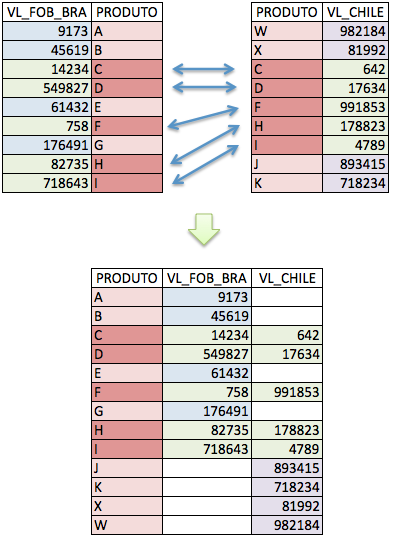
\includegraphics[width=1\linewidth]{imagens/full_join} 

}

\caption{Cruzamento de tabelas}\label{fig:unnamed-chunk-109}
\end{figure}

\begin{Shaded}
\begin{Highlighting}[]
\NormalTok{final4 <-}\StringTok{ }\NormalTok{departamentos }\OperatorTok\StringTok{ }
\StringTok{  }\KeywordTok{full_join}\NormalTok{(empregados, }\DataTypeTok{by =} \KeywordTok{c}\NormalTok{(}\StringTok{'Manager'}\NormalTok{=}\StringTok{'Employee'}\NormalTok{))}

\NormalTok{final4}
\end{Highlighting}
\end{Shaded}

\begin{verbatim}
## # A tibble: 7 x 6
##   Department.x DepartmentName Manager EmployeeName Department.y Salary
##          <int>          <chr>   <int>        <chr>        <int>  <int>
## 1           11     Production       1        Alice           11    800
## 2           12          Sales       4       Daniel           12   1000
## 3           13      Marketing       5       Evelyn           13    800
## 4           14       Research      NA         <NA>           NA     NA
## 5           NA           <NA>       2          Bob           11    600
## 6           NA           <NA>       3        Carla           12    900
## 7           NA           <NA>       6    Ferdinand           21    700
\end{verbatim}

Do resultado desse full join, por exemplo, podemos concluir que não tem
nenhum \emph{Manager} no departamento \emph{Resarch}, da mesma forma os
empregados Bob, Carla e Ferdinand não são \emph{managers} de
departamento nenhum.

\section{Exercícios}\label{exercicios-5}

\begin{enumerate}
\def\labelenumi{\arabic{enumi}.}
\tightlist
\item
  Utilizando as bases de dados do pacote \texttt{nycflights13}, encontre
  a tabela abaixo que mostra quais aeroportos (Origem e Destino) tiveram
  mais voos. Será necessário utilizar o dataframe \texttt{flights} e
  \texttt{airports}. \texttt{Dica:\ primeiro\ descubra\ as\ chaves.}
\end{enumerate}

\begin{verbatim}
## # A tibble: 217 x 3
## # Groups:   Origem [3]
##                 Origem                            Destino   qtd
##                  <chr>                              <chr> <int>
##  1 John F Kennedy Intl                   Los Angeles Intl 11262
##  2          La Guardia    Hartsfield Jackson Atlanta Intl 10263
##  3          La Guardia                 Chicago Ohare Intl  8857
##  4 John F Kennedy Intl                 San Francisco Intl  8204
##  5          La Guardia             Charlotte Douglas Intl  6168
##  6 Newark Liberty Intl                 Chicago Ohare Intl  6100
##  7 John F Kennedy Intl General Edward Lawrence Logan Intl  5898
##  8          La Guardia                         Miami Intl  5781
##  9 John F Kennedy Intl                       Orlando Intl  5464
## 10 Newark Liberty Intl General Edward Lawrence Logan Intl  5327
## # ... with 207 more rows
\end{verbatim}

\begin{enumerate}
\def\labelenumi{\arabic{enumi}.}
\setcounter{enumi}{1}
\tightlist
\item
  Utilizando os dataframes abaixo, chege no resultado a seguir.
\end{enumerate}

\begin{Shaded}
\begin{Highlighting}[]
\NormalTok{participantes <-}\StringTok{ }\KeywordTok{data.frame}\NormalTok{(}
  \DataTypeTok{Nome =} \KeywordTok{c}\NormalTok{(}\StringTok{'Carlos'}\NormalTok{, }\StringTok{'Maurício'}\NormalTok{, }\StringTok{'Ana Maria'}\NormalTok{, }\StringTok{'Rebeca'}\NormalTok{, }\StringTok{'Patrícia'}\NormalTok{),}
  \DataTypeTok{Cidade =} \KeywordTok{c}\NormalTok{(}\StringTok{'Brasília'}\NormalTok{, }\StringTok{'Minas Gerais'}\NormalTok{, }\StringTok{'Goiás'}\NormalTok{, }\StringTok{'São Paulo'}\NormalTok{, }\StringTok{'Ceará'}\NormalTok{),}
  \DataTypeTok{Idade =} \KeywordTok{c}\NormalTok{(}\DecValTok{23}\NormalTok{, }\DecValTok{24}\NormalTok{, }\DecValTok{22}\NormalTok{, }\DecValTok{29}\NormalTok{, }\DecValTok{28}\NormalTok{)}
\NormalTok{)}

\NormalTok{aprovados <-}\StringTok{ }\KeywordTok{data.frame}\NormalTok{(}
  \DataTypeTok{Nome =} \KeywordTok{c}\NormalTok{(}\StringTok{'Carlos'}\NormalTok{, }\StringTok{'Patrícia'}\NormalTok{),}
  \DataTypeTok{Pontuacao =} \KeywordTok{c}\NormalTok{(}\DecValTok{61}\NormalTok{, }\DecValTok{62}\NormalTok{)}
\NormalTok{)}

\NormalTok{eliminados <-}\StringTok{ }\KeywordTok{data.frame}\NormalTok{(}
  \DataTypeTok{Nome =} \KeywordTok{c}\NormalTok{(}\StringTok{'Maurício'}\NormalTok{, }\StringTok{'Ana Maria'}\NormalTok{, }\StringTok{'Rebeca'}\NormalTok{),}
  \DataTypeTok{Pontuacao =} \KeywordTok{c}\NormalTok{(}\DecValTok{49}\NormalTok{, }\DecValTok{48}\NormalTok{, }\DecValTok{48}\NormalTok{)}
\NormalTok{)}

\NormalTok{participantes}
\end{Highlighting}
\end{Shaded}

\begin{verbatim}
##        Nome       Cidade Idade
## 1    Carlos     Brasília    23
## 2  Maurício Minas Gerais    24
## 3 Ana Maria        Goiás    22
## 4    Rebeca    São Paulo    29
## 5  Patrícia        Ceará    28
\end{verbatim}

\begin{Shaded}
\begin{Highlighting}[]
\NormalTok{aprovados}
\end{Highlighting}
\end{Shaded}

\begin{verbatim}
##       Nome Pontuacao
## 1   Carlos        61
## 2 Patrícia        62
\end{verbatim}

\begin{Shaded}
\begin{Highlighting}[]
\NormalTok{eliminados}
\end{Highlighting}
\end{Shaded}

\begin{verbatim}
##        Nome Pontuacao
## 1  Maurício        49
## 2 Ana Maria        48
## 3    Rebeca        48
\end{verbatim}

\begin{verbatim}
## Warning: Column `Nome` joining factors with different levels, coercing to
## character vector
\end{verbatim}

\begin{verbatim}
## Warning: Column `Nome` joining character vector and factor, coercing into
## character vector
\end{verbatim}

\begin{verbatim}
##        Nome       Cidade Idade Pontuacao Resultado
## 1    Carlos     Brasília    23        61  Aprovado
## 2  Maurício Minas Gerais    24        49 Eliminado
## 3 Ana Maria        Goiás    22        48 Eliminado
## 4    Rebeca    São Paulo    29        48 Eliminado
## 5  Patrícia        Ceará    28        62  Aprovado
\end{verbatim}

\chapter{Escrevendo dados}\label{escrevendo-dados}

Já na fase final da sua análise, pode ser que apareça a necessidade de
gerar arquivos: gráficos, relatórios, planilhas, pdf, arquivos de dados,
etc.

Da mesma forma que você consome dados e relatórios, talvez você precise
produzir e divulgar dados e relatórios para outras pessoas analisarem,
ou para publicar.

\section{Escrevendo csv}\label{escrevendo-csv}

O formato mais básico e mais usado mundialmente para envio e recebimento
de dados entre instituições é o \texttt{csv}. Para escrever um arquivo
de dados em csv é muito simples. Utilizaremos uma função do R base para
isso: \texttt{write.table()}

\section{Rdata}\label{rdata}

Caso seja necessário salvar um ou vários objetos para passar para alguém
ou até mesmo para continuar seu trabalho a partir de certo ponto,
pode-se utilizar o formato de dados próprios do R: Rdata.

Veja o seguinte exemplo:

\begin{Shaded}
\begin{Highlighting}[]
\NormalTok{participantes <-}\StringTok{ }\KeywordTok{data.frame}\NormalTok{(}
  \DataTypeTok{Nome =} \KeywordTok{c}\NormalTok{(}\StringTok{'Carlos'}\NormalTok{, }\StringTok{'Maurício'}\NormalTok{, }\StringTok{'Ana Maria'}\NormalTok{, }\StringTok{'Rebeca'}\NormalTok{, }\StringTok{'Patrícia'}\NormalTok{),}
  \DataTypeTok{Cidade =} \KeywordTok{c}\NormalTok{(}\StringTok{'Brasília'}\NormalTok{, }\StringTok{'Minas Gerais'}\NormalTok{, }\StringTok{'Goiás'}\NormalTok{, }\StringTok{'São Paulo'}\NormalTok{, }\StringTok{'Ceará'}\NormalTok{),}
  \DataTypeTok{Idade =} \KeywordTok{c}\NormalTok{(}\DecValTok{23}\NormalTok{, }\DecValTok{24}\NormalTok{, }\DecValTok{22}\NormalTok{, }\DecValTok{29}\NormalTok{, }\DecValTok{28}\NormalTok{)}
\NormalTok{)}

\KeywordTok{save}\NormalTok{(participantes, }\DataTypeTok{file =} \StringTok{'participantes.Rdata'}\NormalTok{)}

\KeywordTok{rm}\NormalTok{(participantes) }\CommentTok{# removendo o objeto}
\end{Highlighting}
\end{Shaded}

Pronto você salvou o objeto \texttt{participantes} no arquivo
\texttt{participantes.Rdata}. Esse arquivo é específico para ser lido
pelo R e interpretado como objeto. Como excluímos o arquivo, tente
exibí-lo para ver o que acontece: erro. Agora vejamos como carregá-lo
novamente no R utilizando o arquivo.

\begin{Shaded}
\begin{Highlighting}[]
\KeywordTok{load}\NormalTok{(}\StringTok{'participantes.Rdata'}\NormalTok{)}

\KeywordTok{str}\NormalTok{(participantes)}
\end{Highlighting}
\end{Shaded}

\begin{verbatim}
## 'data.frame':    5 obs. of  3 variables:
##  $ Nome  : Factor w/ 5 levels "Ana Maria","Carlos",..: 2 3 1 5 4
##  $ Cidade: Factor w/ 5 levels "Brasília","Ceará",..: 1 4 3 5 2
##  $ Idade : num  23 24 22 29 28
\end{verbatim}

\section{Escrevendo outros tipos de
arquivos}\label{escrevendo-outros-tipos-de-arquivos}

Outra forma bastante importante de escrever dados é em planilhas: o
famoso Excel. Recomendo conhecer o pacote \texttt{openxlsx}. É um pacote
que lê e escreve excel sem nenhuma dependência de Java, que pode acabar
dando muita dor de cabeça para manter e normalmente consome bastante
memória. Para windows o \texttt{openxlsx} precisa do \texttt{Rtools}:
\url{https://cran.r-project.org/bin/windows/Rtools/}. Recomendamos
conhecer e experimentar esse pacote, com ele é possível criação de
planilhas bem acabadas, com cores e formatações complexas.

Outra forma de escrita de dados é utilizando o RMarkdown, mas esse
formato merece um capítulo específico para detalhar seu uso.

\section{Exercícios}\label{exercicios-6}

.1 Escolha qualquer dataframe já trabalhado até agora e escreva-o em
csv.

.2 Experimente algo semelhante ao exemplo: escolha qualquer dataframe,
save-o como Rdata, remova-o com o \texttt{rm()} em seguida carrege
novamente com o \texttt{load()}

\chapter{Obtendo dados}\label{obtendo-dados}

A base da ciência de dados é, obviamente, o DADO. Portanto, é
fundamental sempre ter boas fontes de dados. Se você der sorte,
conseguirá dados estruturados para iniciar sua análise. Porém,
eventualmente precisará recorrer a fontes de dados não estruturados ou
semi-estruturados.

Muito provavelmente você algum dia precisará recorrer a uma API de
dados, ou até mesmo utilizar técnicas de Web Scrapping para obter dados
diretamente em um próprio site.

\section{API}\label{api}

API (\emph{Application Programming Interface}), é uma forma de
comunicação de dados mais apropriada para trocas de informações entre
softwares. Normalmente APIs trocam dados em formato hierárquico. Os dois
formatos hierárquicos mais comuns são JSON (Javascript Object Notation)
e XML (eXtensible Markup Language).

Para obter e utilizar dados de API em R recomendamos a utilização do
pacote \texttt{jsonlite}.

\begin{Shaded}
\begin{Highlighting}[]
\KeywordTok{library}\NormalTok{(jsonlite)}
\end{Highlighting}
\end{Shaded}

A seguir apresentaremos alguns exemplos de APIs e seu uso. Existem
diversas APIs e formas de consumí-las, portanto não iremos exaurir nesse
texto todas as possibilidades de uso de APIs. O principal é entender
APIs como uma fonte rica de dados que pode ser explorada em suas
análises.

No exemplo a seguir utilizamos a API do github (portal para
repositórios) e veremos quais os repositórios do Hadley Wickham

\begin{Shaded}
\begin{Highlighting}[]
\NormalTok{hadley.rep <-}\StringTok{ }\NormalTok{jsonlite}\OperatorTok{::}\KeywordTok{fromJSON}\NormalTok{(}\StringTok{"https://api.github.com/users/hadley/repos"}\NormalTok{)}

\KeywordTok{dim}\NormalTok{(hadley.rep)}
\end{Highlighting}
\end{Shaded}

\begin{verbatim}
## [1] 30 71
\end{verbatim}

\begin{Shaded}
\begin{Highlighting}[]
\KeywordTok{head}\NormalTok{(hadley.rep[,}\KeywordTok{c}\NormalTok{(}\StringTok{'name'}\NormalTok{, }\StringTok{'description'}\NormalTok{)], }\DecValTok{15}\NormalTok{)}
\end{Highlighting}
\end{Shaded}

\begin{verbatim}
##                     name
## 1  15-state-of-the-union
## 2      15-student-papers
## 3               500lines
## 4                  adv-r
## 5                appdirs
## 6             assertthat
## 7              babynames
## 8         beautiful-data
## 9                  bench
## 10                bigvis
## 11        bigvis-infovis
## 12        boxplots-paper
## 13                 broom
## 14               builder
## 15      building-permits
##                                                                                          description
## 1                                                                                               <NA>
## 2                                              Graphics & computing student paper winners @ JSM 2015
## 3                                                                                  500 Lines or Less
## 4                                                                     Advanced R programming: a book
## 5  A small Python module for determining appropriate platform-specific dirs, e.g. a "user data dir".
## 6                                                                     User friendly assertions for R
## 7                                              An R package contain all baby names data from the SSA
## 8                                                                    Book chapter for beautiful data
## 9                                                                            Bechmarking tools for R
## 10                        Exploratory data analysis for large datasets (10-100 million observations)
## 11                       Paper describing the bigvis package and framework submitted to Infovis 2013
## 12                                                                                              <NA>
## 13                                      Convert statistical analysis objects from R into tidy format
## 14                                    Provide a simple way to create XML markup and data structures.
## 15                                               Code & data accompanying "whole-game" youtube video
\end{verbatim}

Outra exemplo de API muito interessante é o portal de dados abertos da
câmara dos deputados, eles possuem diversas APIs para consultar os dados
do processo legislativo. Veja o exemplo a seguir que resgata as
proposições utilizando API:

\begin{Shaded}
\begin{Highlighting}[]
\NormalTok{proposicoes <-}\StringTok{ }\NormalTok{jsonlite}\OperatorTok{::}\KeywordTok{fromJSON}\NormalTok{(}\StringTok{"https://dadosabertos.camara.leg.br/api/v2/proposicoes"}\NormalTok{)}

\KeywordTok{head}\NormalTok{(proposicoes}\OperatorTok{$}\NormalTok{dados }\OperatorTok\StringTok{ }\KeywordTok{select}\NormalTok{(siglaTipo, numero, ano, ementa))}
\end{Highlighting}
\end{Shaded}

\begin{verbatim}
##   siglaTipo numero  ano
## 1       PEC    454 1997
## 2        PL      6 1995
## 3        PL    125 1999
## 4        PL    220 1995
## 5        PL    227 1995
## 6        PL    246 1995
##                                                                                                                                                                                                                            ementa
## 1                                                                                                                                     Altera o art. 144 da Constituição Federal para criar o Fundo Nacional de Segurança Pública.
## 2                                                       Altera a Lei nº 8.666, de 21 de junho de 1993, que regulamenta o artigo 37, Inciso XXI da Constituição Federal, institui normas para licitações e dá outras providências.
## 3                                                                                                                                                                      Estabelece a obrigatoriedade do trabalho para os detentos.
## 4 Altera dispositivos da Lei nº 8.666, de 21 de junho de 1993, que "regulamenta o artigo 37, inciso XXI, da Constituição Federal, institui normas para licitações e contratos da Administração Pública e dá outras providências".
## 5 Altera dispositivos da Lei nº 8.666, de 21 de junho de 1993, que "regulamenta o artigo 37, inciso XXI, da Constituição Federal, institui normas para licitações e contratos de Administração Pública e dá outras providências".
## 6 Altera dispositivos da Lei nº 8.666, de 21 de junho de 1993, que "regulamenta o artigo 37, inciso XXI, da Constituição Federal, institui normas para licitações e contratos da Administração Pública e dá outras providências".
\end{verbatim}

Hoje em dia todas as redes sociais possuem APIs para consumir os dados
dos usuários e postagens. Normalmente essas APIs pedem um cadastro
anterior (apesar de gratuitas em sua maior parte). O R possui diversos
pacotes para consumir APIs interessantes:

\begin{itemize}
\tightlist
\item
  Quandl: pacote que fornece diversos dados econômicos de diversos
  países
\item
  Rfacebook: pacote que facilita o uso da API do facebook (requer
  cadastro prévio)
\item
  twitterR: pacote que facilita o uso da API do twitter (requer cadastro
  prévio)
\item
  ggmap: pacote que facilita o uso da API do google maps
\end{itemize}

Como dito, a lista não é exaustiva. Sempre procure por APIs para obter
dados que possam enriquecer suas análises.

\section{Web Scrapping}\label{web-scrapping}

Eventualmente você não terá facilmente dados estruturados, nem terá uma
API com os dados que procura. Nesses casos pode ser que um próprio site
da internet seja sua fonte de dados. Para isso utiliza-se técnicas
chamadas de Web Scrapping.

Sites da internet são construídos utilizando uma linguagem que é
interpretada pelos browsers: HTML (\emph{HyperText Markup Language}). É
uma linguagem que trabalha com tags de forma hierárquica. Nesse site
você pode aprender um pouco mais o que é HTML
\url{http://www.w3schools.com/html/tryit.asp?filename=tryhtml_basic_document}

Existe um pacote em R que facilita muito o cosumo de dados em HTML:
\texttt{rvest}, criado tamém por Hadley Wickham. O \texttt{rvest} mapeia
os elementos HTML (tabs) de uma página web e facilita a ``navegação'' do
R por esses nós da árvore do HTML. Veja o exemplo a seguir:

\begin{Shaded}
\begin{Highlighting}[]
\KeywordTok{library}\NormalTok{(rvest)}

\NormalTok{html <-}\StringTok{ }\KeywordTok{read_html}\NormalTok{(}\StringTok{"https://pt.wikipedia.org/wiki/Lista_de_redes_de_televis%C3%A3o_do_Brasil"}\NormalTok{)}

\NormalTok{html.table <-}\StringTok{ }\NormalTok{html }\OperatorTok\StringTok{ }\KeywordTok{html_nodes}\NormalTok{(}\StringTok{"table"}\NormalTok{)}
\NormalTok{dados <-}\StringTok{ }\NormalTok{html.table[[}\DecValTok{1}\NormalTok{]] }\OperatorTok\StringTok{ }\KeywordTok{html_table}\NormalTok{()}

\NormalTok{dados <-}\StringTok{ }\NormalTok{dados }\OperatorTok\StringTok{ }
\StringTok{  }\KeywordTok{select}\NormalTok{(}\OperatorTok{-}\StringTok{`}\DataTypeTok{Lista de emissoras}\StringTok{`}\NormalTok{)}

\KeywordTok{head}\NormalTok{(dados)}
\end{Highlighting}
\end{Shaded}

Otivemos todo o HTML da página, mapeamos os nós de tabela (table) e
pegamos seu conteúdo. A partir daí trata-se de um dataframe normal que
pode ser manipulado com o dplyr.

\section{Exercícios}\label{exercicios-7}

\begin{enumerate}
\def\labelenumi{\arabic{enumi}.}
\item
  Obtenha a tabela exibida em
  \url{http://globoesporte.globo.com/futebol/brasileirao-serie-a/} e
  chegue no seguinte resultado:
\item
  Escolha um site do seu interesse e faça um dataframe com uma parte do
  seu conteúdo (tabelas, listas, etc\ldots{})
\end{enumerate}

\chapter{Visualizações de dados (ggplot2)}\label{ggplot2}

O \texttt{ggplot2} é mais um pacote desenvolvido pelo Hadley Wickham, o
criador, por exemplo, do \texttt{tidyr} e do \texttt{dplyr}. A ideia do
pacote, ainda que com algumas modificações, vem de uma obra chamada
\href{https://www.amazon.com/Grammar-Graphics-Statistics-Computing/dp/0387245448}{\emph{The
Grammar of Graphics}}, que é uma maneira de descrever um gráfico a
partir dos seus componentes. Dessa forma, teoricamente, ficaria mais
fácil entender a construção de gráficos mais complexos.

O \texttt{ggplot2} é estruturado de forma que a ``gramática'' seja
utilizada para um gráfico a partir de múltiplas camadas. As camadas
serão formadas por dados, mapeamentos estéticos, transformações
estatísticas dos dados, objetos geométricos (pontos, linhas, barras
etc.) e ajuste de posicionamento. Além disso, existem outros componentes
como os sistemas de coordenadas (cartesiano, polar, mapa etc.) e, se for
o caso, divisões do gráfico em subplots (\emph{facet}). Um simples
exemplo de múltiplas camadas seria um gráfico de pontos adicionado de
uma curva de ajustamento.

Uma forma geral (template) para entender a estrutura do ggplot2, segundo
o próprio Hadley Wickhan no livro
\href{http://r4ds.had.co.nz/data-visualisation.html\#the-layered-grammar-of-graphics}{R
for Data Science}, é a seguinte:

\begin{verbatim}
ggplot(data = <DATA>) + 
  <GEOM_FUNCTION>(
     mapping = aes(<MAPPINGS>),
     stat = <STAT>, 
     position = <POSITION>
  ) +
  <COORDINATE_FUNCTION> +
  <FACET_FUNCTION> # dividir o gráfico em subplots
\end{verbatim}

A ideia é que todo gráfico pode ser representado por essa forma. No
entanto, na criação de um gráfico, não é necessário especificar todas as
partes acima. O ggplot2 já oferece um padrão para o sistema de
coordenadas, para o \texttt{stat} e \texttt{position}. O \texttt{facet}
(subplot) só será utilizado quando necessário.

Além disso, existem as escalas que são utilizadas para controlar o
mapeamento dos dados em relação aos atributos estéticos do gráfico. Por
exemplo, suponha que no seu gráfico existe uma coluna que é uma variável
categórica com 3 classes possíveis, e as cores do objeto geométrico
estão associadas a essa variável. Automaticamente, o ggplot2 vai definir
uma cor pra cada classe. No entanto, você pode alterar a escala de cores
para ter controle sobre elas. O mesmo vale para os valores apresentados
nos eixos x e y.

Uma observação importante é que, apesar de os dados estarem na função
\texttt{ggplot()} (\texttt{\textless{}DATA\textgreater{}}), eles também
podem ser incluídos diretamente em cada objeto geométrico. Isso será
útil quando for necessário criar uma nova camada a partir de dados
diferentes daqueles que estão inicialmente nos gráficos.

Dessa forma, incorporando essas observações, um template estendido seria
o abaixo:

\begin{verbatim}
ggplot(data = <DATA>) + 
  <GEOM_FUNCTION>(
     mapping = aes(<MAPPINGS>),
     stat = <STAT>, 
     position = <POSITION>,
     data = <DATA> # pode receber os dados diretamente
  ) +
  <SCALE_FUNCTION> + # uma para cada elemento estético
  <COORDINATE_FUNCTION> +
  <FACET_FUNCTION> # dividir o gráfico em subplots
\end{verbatim}

Também é importante ressaltar que, como todo sistema de gráficos, é
possível alterar todos os títulos e rótulos do gráfico, além de controle
sobre características do tema do gráfico (cor do fundo, estilo da fonte,
tamanho da fonte etc).

Para quebrar a barreira inicial, vamos criar um exemplo por partes:

\begin{Shaded}
\begin{Highlighting}[]
\KeywordTok{library}\NormalTok{(ggplot2)}
\KeywordTok{data}\NormalTok{(}\StringTok{"mtcars"}\NormalTok{)}

\CommentTok{# Inicia o plot}
\NormalTok{g <-}\StringTok{ }\KeywordTok{ggplot}\NormalTok{(mtcars)}

\CommentTok{# Adicionar pontos (geom_point) e}
\CommentTok{# vamos mapear variáveis a elemetos estéticos dos pontos}
\CommentTok{# Size = 3 define o tamanho de todos os pontos}
\NormalTok{g <-}\StringTok{ }\NormalTok{g }\OperatorTok{+}
\StringTok{  }\KeywordTok{geom_point}\NormalTok{(}\KeywordTok{aes}\NormalTok{(}\DataTypeTok{x =}\NormalTok{ hp, }\DataTypeTok{y =}\NormalTok{ mpg, }\DataTypeTok{color =} \KeywordTok{factor}\NormalTok{(am)),}
             \DataTypeTok{size =} \DecValTok{3}\NormalTok{)}

\CommentTok{# Altera a escala de cores}
\NormalTok{g <-}\StringTok{ }\NormalTok{g }\OperatorTok{+}
\StringTok{  }\KeywordTok{scale_color_manual}\NormalTok{(}\StringTok{"Automatic"}\NormalTok{,}
                     \DataTypeTok{values =} \KeywordTok{c}\NormalTok{(}\StringTok{"red"}\NormalTok{, }\StringTok{"blue"}\NormalTok{),}
                     \DataTypeTok{labels =} \KeywordTok{c}\NormalTok{(}\StringTok{"No"}\NormalTok{, }\StringTok{"Yes"}\NormalTok{))}

\CommentTok{# Rótulos (títulos)}
\NormalTok{g <-}\StringTok{ }\NormalTok{g }\OperatorTok{+}
\StringTok{  }\KeywordTok{labs}\NormalTok{(}\DataTypeTok{title =} \StringTok{'Relação entre consumo, potência e tipo de câmbio'}\NormalTok{,}
       \DataTypeTok{y =} \StringTok{'Consumo'}\NormalTok{,}
       \DataTypeTok{x =} \StringTok{'Potência')}

\StringTok{g}
\end{Highlighting}
\end{Shaded}

\begin{center}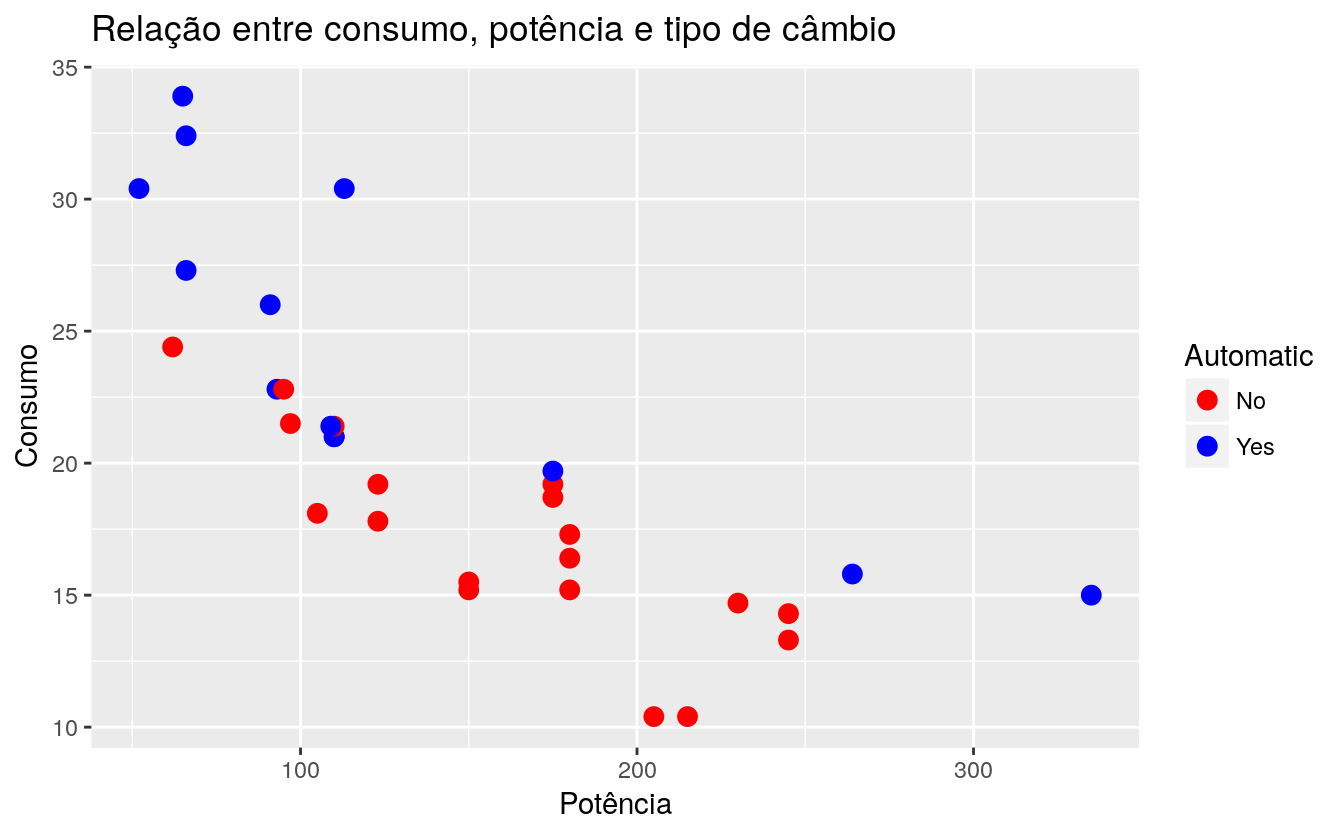
\includegraphics[width=1\linewidth]{bookdown-demo_files/figure-latex/unnamed-chunk-125-1} \end{center}

Note que o gráfico poderia ser criado com um bloco único de código:

\begin{Shaded}
\begin{Highlighting}[]
\KeywordTok{ggplot}\NormalTok{(mtcars) }\OperatorTok{+}
\StringTok{  }\KeywordTok{geom_point}\NormalTok{(}\KeywordTok{aes}\NormalTok{(}\DataTypeTok{x =}\NormalTok{ hp, }\DataTypeTok{y =}\NormalTok{ mpg, }\DataTypeTok{color =} \KeywordTok{factor}\NormalTok{(am)),}
             \DataTypeTok{size =} \DecValTok{3}\NormalTok{) }\OperatorTok{+}
\StringTok{  }\KeywordTok{scale_color_manual}\NormalTok{(}\StringTok{"Automatic"}\NormalTok{,}
                     \DataTypeTok{values =} \KeywordTok{c}\NormalTok{(}\StringTok{"red"}\NormalTok{, }\StringTok{"blue"}\NormalTok{),}
                     \DataTypeTok{labels =} \KeywordTok{c}\NormalTok{(}\StringTok{"No"}\NormalTok{, }\StringTok{"Yes"}\NormalTok{)) }\OperatorTok{+}
\StringTok{  }\KeywordTok{labs}\NormalTok{(}\DataTypeTok{title =} \StringTok{'Relação entre consumo, potência e tipo de câmbio'}\NormalTok{,}
       \DataTypeTok{y =} \StringTok{'Consumo'}\NormalTok{,}
       \DataTypeTok{x =} \StringTok{'Potência')}
\end{Highlighting}
\end{Shaded}

\begin{center}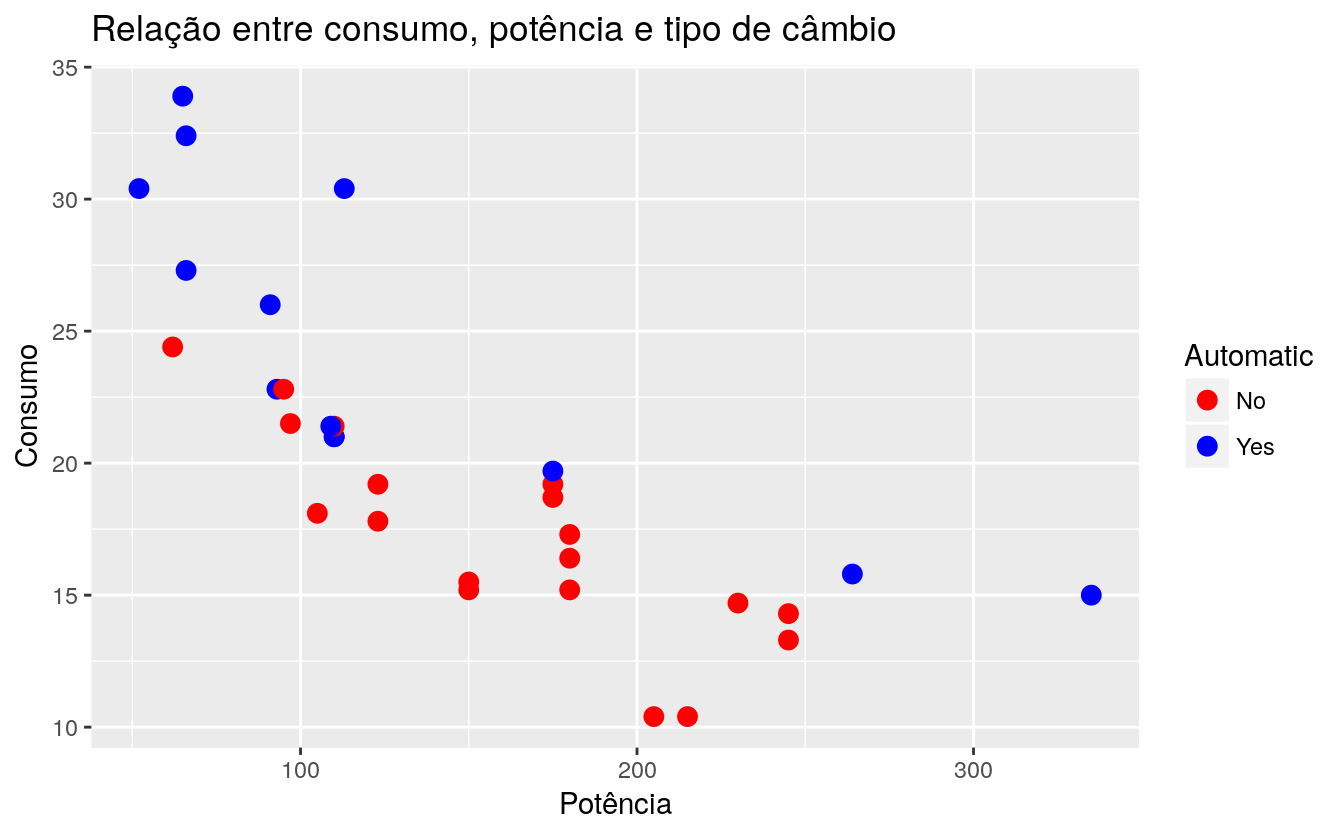
\includegraphics[width=1\linewidth]{bookdown-demo_files/figure-latex/unnamed-chunk-126-1} \end{center}

Iremos detalhar cada parte do gráfico, mas vale falar rapidamente sobre
o código acima. Primeiramente, passamos um conjunto de dados para o
ggplot. Depois, adicionamos uma camada de pontos, mapeando as variáveis
\texttt{hp} e \texttt{mpg} para as posições de cada ponto nos eixos
\texttt{x} e \texttt{y}, respectivamente, e a variável \texttt{am} para
a cor de cada ponto. Adicionalmente, alteramos a escala de cor,
definindo seu título, os rótulos (\texttt{labels}) e os valores
(\texttt{values}) para as cores. Por fim, definimos os títulos/rótulos
do gráfico.

Nas próximas seções, iremos falar com mais detalhes de cada componente.
Começando pelo mapeamento estético.

\section{Mapeamento Estético}\label{mapeamento-estetico}

O mapeamento estético é o mapeamento de variáveis dos dados às
características visuais dos objetos geométricos (pontos, barras, linhas
etc.). Isso é feito a partir da função \texttt{aes()}. E quais são as
características visuais de um objeto geométrico? Abaixo segue uma lista
não exaustiva:

\begin{itemize}
\tightlist
\item
  Posição (\texttt{x} e \texttt{y});
\item
  Cor (\texttt{color});
\item
  Tamanho (\texttt{size});
\item
  Preenchimento (\texttt{fill});
\item
  Transparência (\texttt{alpha});
\item
  Texto (\texttt{label});
\end{itemize}

Como vimos no exemplo acima, mapeamos três variáveis para três
características visuais de cada ponto: posição \texttt{x}, posição
\texttt{y} e cor. Nos próximos exemplos, outros elementos estéticos
serão utilizados, conforme o objeto geométrico selecionado.

\section{Objetos geométricos}\label{objetos-geometricos}

Os objetos geométricos começam com a expressão \texttt{geom\_} e são
seguidos pelo tipo de objeto. Por exemplo, \texttt{geom\_point()} para
pontos e \texttt{geom\_bar()} para barras. A tabela abaixo apresenta os
tipos de objetos geométricos utilizados para criar alguns tipos de
gráficos populares.

\begin{longtable}[]{@{}cc@{}}
\toprule
Tipo & Objeto Geométrico\tabularnewline
\midrule
\endhead
Dispersão (scatterplot) & \texttt{geom\_point()}\tabularnewline
Gráfico de bolhas & \texttt{geom\_point()}\tabularnewline
Gráfico de barras & \texttt{geom\_bar()} e
\texttt{geom\_col()}\tabularnewline
Histograma & \texttt{geom\_histogram()}\tabularnewline
Boxplot & \texttt{geom\_boxplot()}\tabularnewline
Densidade & \texttt{geom\_density()}\tabularnewline
Gráfico de linhas & \texttt{geom\_line()}\tabularnewline
\bottomrule
\end{longtable}

Nesse material, os principais tipos de objetos geométricos serão
demonstrados a partir de exemplos. A lista completa de objetos
geométricos e as descrições dos argumentos estão na
\href{http://docs.ggplot2.org/current/}{documentação} do
\texttt{ggplot2}.

É importante saber que um gráfico do ggplot2 pode ter mais de um objeto
geométrico, cada um formando uma camada. Por exemplo, uma camada pontos
e outra de linhas que conectam os pontos.

Vamos primeiramente criar uma gráfico com pontos a partir dos dados
\texttt{mtcars}. Use \texttt{?mtcars} para mais detalhes.

\begin{Shaded}
\begin{Highlighting}[]
\NormalTok{g1 <-}\StringTok{ }\KeywordTok{ggplot}\NormalTok{(mtcars, }\KeywordTok{aes}\NormalTok{(}\DataTypeTok{y =}\NormalTok{ mpg, }\DataTypeTok{x =}\NormalTok{ disp)) }\OperatorTok{+}
\StringTok{  }\KeywordTok{geom_point}\NormalTok{()}

\NormalTok{g1}
\end{Highlighting}
\end{Shaded}

\begin{center}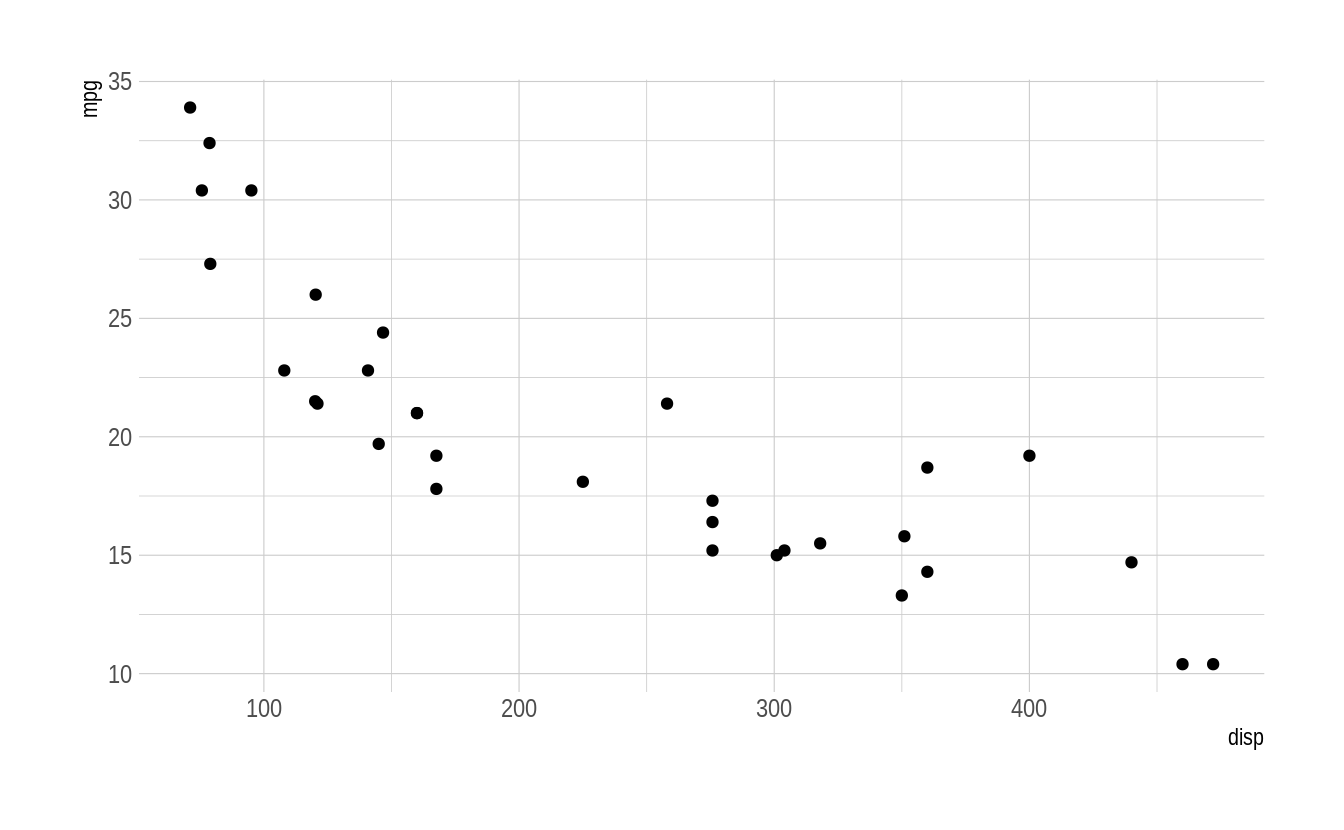
\includegraphics[width=1\linewidth]{bookdown-demo_files/figure-latex/unnamed-chunk-127-1} \end{center}

\begin{quote}
Note que o \texttt{aes()} está sendo usado diretamente na função
\texttt{ggplot()}, e não no objeto geométrico. O que isso significa? O
mapeamento estético definido na função \texttt{ggplot()} é global. Ou
seja, é aplicado para todos os objetos geométricos daquele gráfico, a
menos que seja explicitado novamente em alguma camada.
\end{quote}

Para finalizar essa breve introdução a objetos geométricos, vamos
adicionar mais uma camada ao gráfico:

\begin{Shaded}
\begin{Highlighting}[]
\KeywordTok{library}\NormalTok{(dplyr)}
\NormalTok{mtcars <-}\StringTok{ }\NormalTok{mtcars }\OperatorTok\StringTok{ }
\StringTok{  }\KeywordTok{mutate}\NormalTok{(}\DataTypeTok{name =} \KeywordTok{rownames}\NormalTok{(mtcars))}
\KeywordTok{ggplot}\NormalTok{(mtcars, }\KeywordTok{aes}\NormalTok{(}\DataTypeTok{y =}\NormalTok{ mpg, }\DataTypeTok{x =}\NormalTok{ disp)) }\OperatorTok{+}
\StringTok{  }\KeywordTok{geom_point}\NormalTok{() }\OperatorTok{+}
\StringTok{  }\KeywordTok{geom_smooth}\NormalTok{()}
\end{Highlighting}
\end{Shaded}

\begin{center}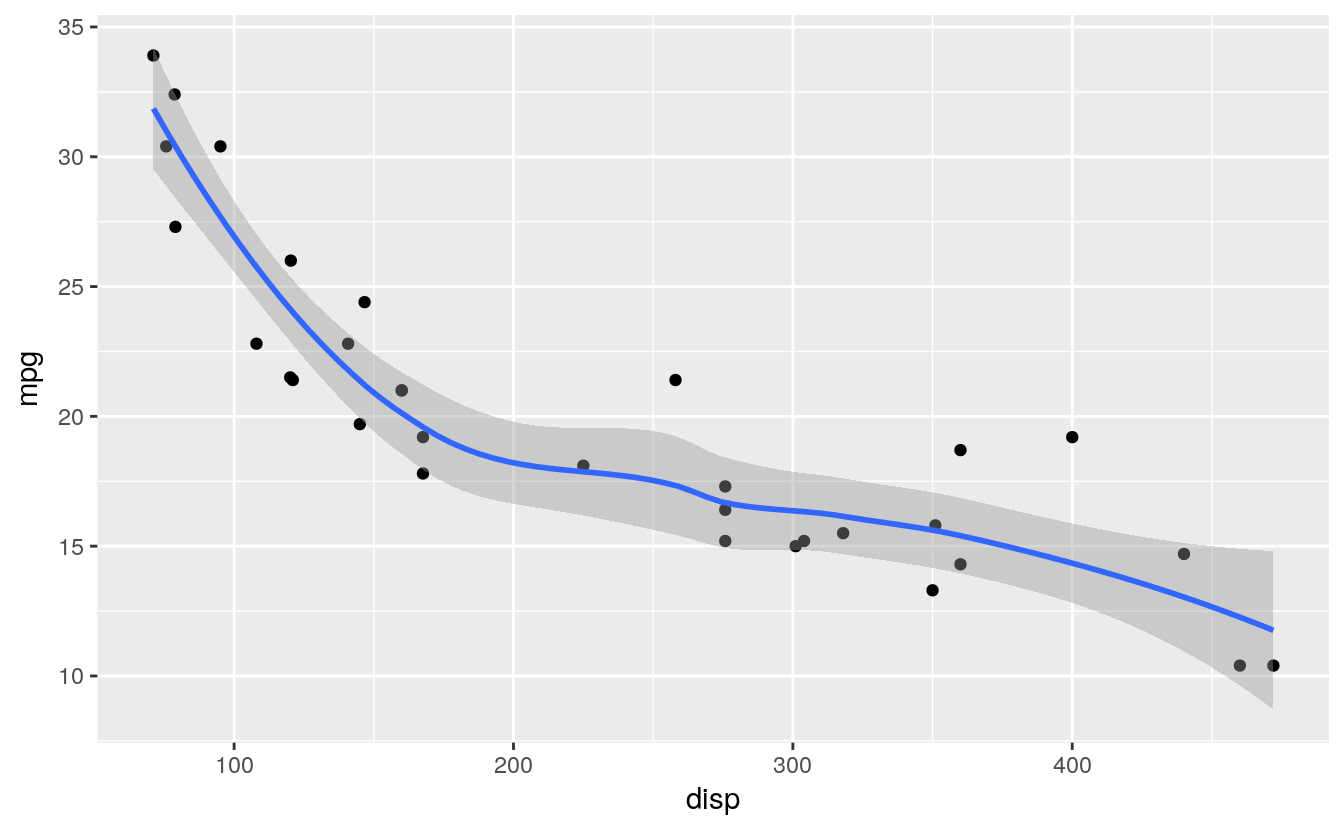
\includegraphics[width=1\linewidth]{bookdown-demo_files/figure-latex/unnamed-chunk-128-1} \end{center}

No caso, adicionamos uma curva de ajustamento aos dados que tem o
objetivo de evidenciar um padrão nos dados.

\section{Escalas}\label{escalas}

O controle sobre as escalas do gráfico é fundamental no ajuste de um
gráfico. Em geral, o ggplot2, como outros pacotes gráficos, fornecem as
escalas automaticamente, não sendo necessário o entendimento de como
controlar esse componente. No entanto, se o interesse é ter controle
sobre todos os aspectos de um gráfico, esse componente é fundamental.

Veja o gráfico abaixo:

\begin{Shaded}
\begin{Highlighting}[]
\KeywordTok{ggplot}\NormalTok{(iris, }\KeywordTok{aes}\NormalTok{(}\DataTypeTok{x =}\NormalTok{ Petal.Length, }\DataTypeTok{y =}\NormalTok{ Petal.Width, }\DataTypeTok{color =}\NormalTok{ Species)) }\OperatorTok{+}
\StringTok{  }\KeywordTok{geom_point}\NormalTok{()}
\end{Highlighting}
\end{Shaded}

\begin{center}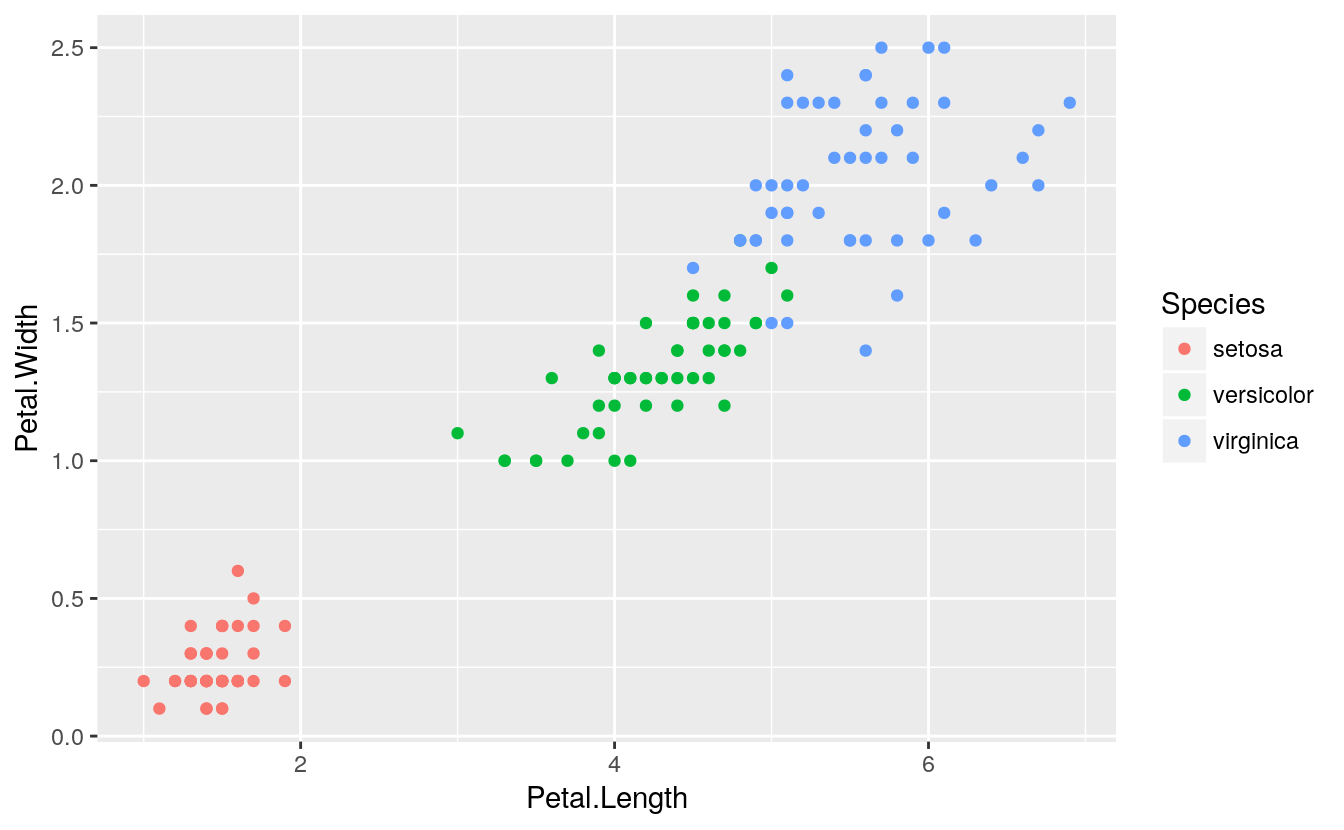
\includegraphics[width=1\linewidth]{bookdown-demo_files/figure-latex/unnamed-chunk-129-1} \end{center}

Note que a cor está mapeada para a variável \texttt{Species}. O
\texttt{ggplot2} automaticamente criou a seguinte escala:

\begin{longtable}[]{@{}cc@{}}
\toprule
Species & Cor\tabularnewline
\midrule
\endhead
setosa & Vermelho\tabularnewline
versicolor & Verde\tabularnewline
virginica & azul\tabularnewline
\bottomrule
\end{longtable}

Todavia, é comum haver interesse em alterar essas cores, ou seja,
alterar a escala de cor. Como fazer isso no ggplot2? Podemos usar, por
exemplo, a função \texttt{scale\_color\_manual()}.

\begin{Shaded}
\begin{Highlighting}[]
\KeywordTok{ggplot}\NormalTok{(iris, }\KeywordTok{aes}\NormalTok{(}\DataTypeTok{x =}\NormalTok{ Petal.Length, }\DataTypeTok{y =}\NormalTok{ Petal.Width, }\DataTypeTok{color =}\NormalTok{ Species)) }\OperatorTok{+}
\StringTok{  }\KeywordTok{geom_point}\NormalTok{() }\OperatorTok{+}
\StringTok{  }\KeywordTok{scale_color_manual}\NormalTok{(}\DataTypeTok{values =} \KeywordTok{c}\NormalTok{(}\StringTok{"orange"}\NormalTok{, }\StringTok{"black"}\NormalTok{, }\StringTok{"red"}\NormalTok{))}
\end{Highlighting}
\end{Shaded}

\begin{center}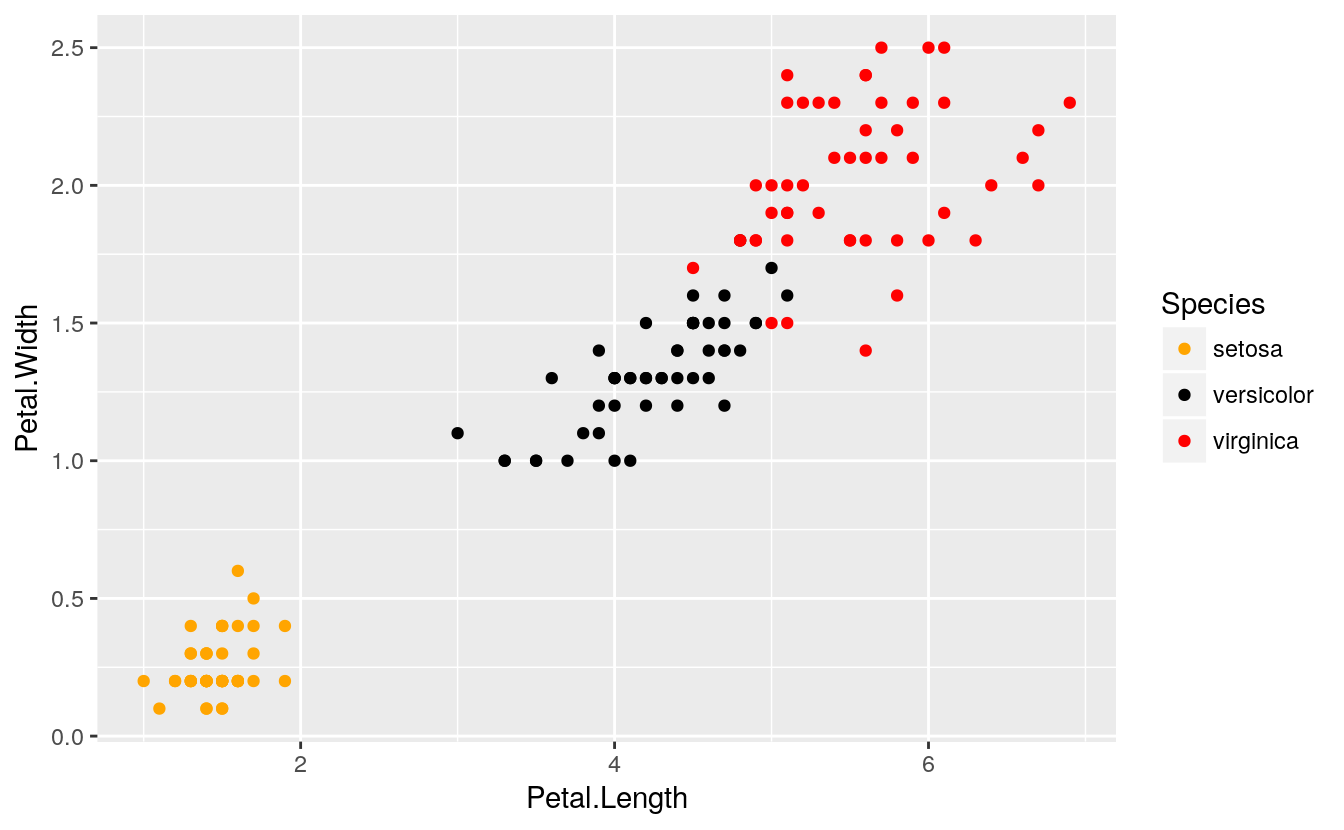
\includegraphics[width=1\linewidth]{bookdown-demo_files/figure-latex/unnamed-chunk-130-1} \end{center}

Usamos a função \texttt{scale\_color\_manual()} em razão da variável
\texttt{Species} ser categórica. Para o ggplot2, dados categóricos são
discretos, e a função citada permite criar uma escala discreta
customizada. No entanto, essa não é a única função para controlar escala
de cor. Existem outras como \texttt{scale\_color\_discrete()},
\texttt{scale\_color\_continuous()}, \texttt{scale\_color\_gradient()}
etc. A utilização de cada função depende do tipo de dado que está
associado ao elemento estético \texttt{color}. Adiante, entraremos em
mais detalhes sobre os tipos de dados.

As funções utilizadas para controlar as escalas dos elementos de um
gráfico do ggplot2 seguem um padrão. Todas iniciam-se com
\texttt{scale\_}, depois o nome do elemento estético (color, fill, x
etc.) e, por fim, o tipo/nome da escala que será aplicada.

Abaixo, continuamos o exemplo anterior, alterando as escalas dos eixos x
e y. Note que as variáveis \texttt{Petal.Length} e \texttt{Petal.Width}
são variáveis numéricas/contínuas. Dessa forma, iremos utilizar as
funções \texttt{scale\_x\_continuous()} e
\texttt{scale\_y\_continuous()}:

\begin{Shaded}
\begin{Highlighting}[]
\KeywordTok{ggplot}\NormalTok{(iris, }\KeywordTok{aes}\NormalTok{(}\DataTypeTok{x =}\NormalTok{ Petal.Length, }\DataTypeTok{y =}\NormalTok{ Petal.Width, }\DataTypeTok{color =}\NormalTok{ Species)) }\OperatorTok{+}
\StringTok{  }\KeywordTok{geom_point}\NormalTok{() }\OperatorTok{+}
\StringTok{  }\KeywordTok{scale_color_manual}\NormalTok{(}\DataTypeTok{values =} \KeywordTok{c}\NormalTok{(}\StringTok{"orange"}\NormalTok{, }\StringTok{"black"}\NormalTok{, }\StringTok{"red"}\NormalTok{)) }\OperatorTok{+}
\StringTok{  }\KeywordTok{scale_x_continuous}\NormalTok{(}\DataTypeTok{name =} \StringTok{"Petal Length"}\NormalTok{, }\DataTypeTok{breaks =} \DecValTok{1}\OperatorTok{:}\DecValTok{7}\NormalTok{) }\OperatorTok{+}\StringTok{ }
\StringTok{  }\KeywordTok{scale_y_continuous}\NormalTok{(}\DataTypeTok{name =} \StringTok{"Petal Width"}\NormalTok{, }\DataTypeTok{breaks =} \DecValTok{0}\OperatorTok{:}\DecValTok{3}\NormalTok{, }\DataTypeTok{limits =} \KeywordTok{c}\NormalTok{(}\DecValTok{0}\NormalTok{, }\DecValTok{3}\NormalTok{))}
\end{Highlighting}
\end{Shaded}

\begin{center}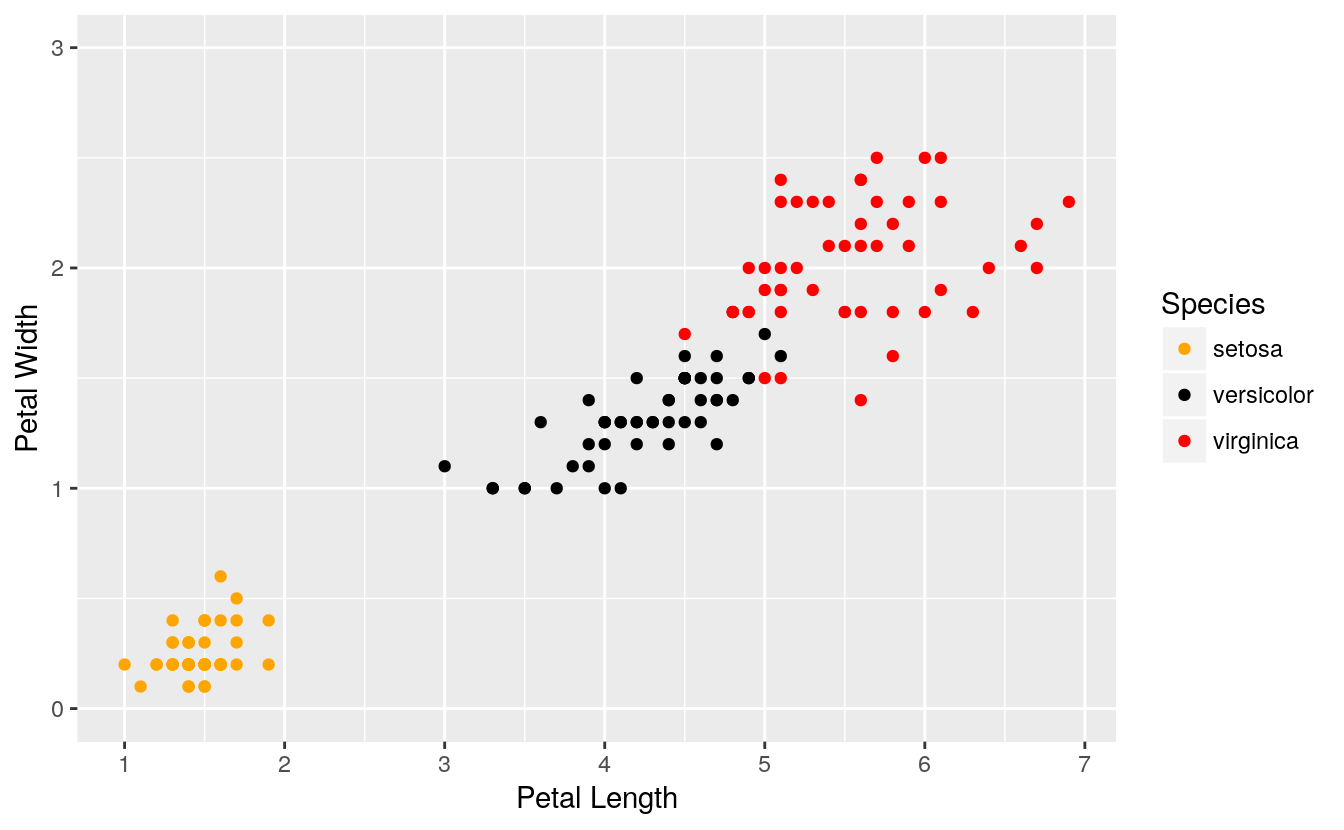
\includegraphics[width=1\linewidth]{bookdown-demo_files/figure-latex/unnamed-chunk-131-1} \end{center}

No gráfico acima, definimos quais seriam os pontos em que rótulos
deveriam ser exibidos em cada eixo. Além disso, no eixo y, definimos que
o limites seriam 0 e 3.

\subsection{Tipos de Variáveis}\label{tipos-de-variaveis}

Para melhor uso das escalas, é preciso saber o tipo de variável que foi
mapeado para cada elemento estético. Vamos rapidamente montar essa
relação:

\begin{longtable}[]{@{}ccc@{}}
\toprule
Classe & Exemplo & Tipo no ggplot2\tabularnewline
\midrule
\endhead
numeric & seq(0, 1, length.out = 10) & continuous\tabularnewline
integer & 1L:10L & continuous ou discrete\tabularnewline
character & c(``Sim'', ``Não'') & discrete\tabularnewline
factor & factor(c(``Sim'', ``Não'')) & discrete\tabularnewline
date & seq(as.Date(``2000/1/1''), by = ``month'', length.out = 12) &
date\tabularnewline
\bottomrule
\end{longtable}

Lembre-se que o padrão do ggplot é \texttt{scale\_}, depois o nome do
elemento estético (color, fill, x etc.) e, por fim, o tipo/nome da
escala que será aplicada. É importante que o usuário saiba o tipo de
dado, pois assim saberá com mais facilidade qual é o tipo de escala que
deve ser escolhido.

Vamos na sequência entrar em mais detalhes para escalas dos eixos
(\texttt{x} e \texttt{y}) e de cores. Espera-se que a intuição
desenvolvida a partir dos exemplos das escalas para esses elementos
estéticos seja útil para os demais elementos estéticos.

\subsection{Eixos}\label{eixos}

\subsubsection{Variáveis Contínuas}\label{variaveis-continuas}

\begin{Shaded}
\begin{Highlighting}[]
\KeywordTok{scale_x_continuous}\NormalTok{(}\DataTypeTok{name =} \KeywordTok{waiver}\NormalTok{(), }\DataTypeTok{breaks =} \KeywordTok{waiver}\NormalTok{(), }\DataTypeTok{minor_breaks =} \KeywordTok{waiver}\NormalTok{(),}
                   \DataTypeTok{labels =} \KeywordTok{waiver}\NormalTok{(), }\DataTypeTok{limits =} \OtherTok{NULL}\NormalTok{, }\DataTypeTok{expand =} \KeywordTok{waiver}\NormalTok{(),}
                   \DataTypeTok{oob =}\NormalTok{ censor, }\DataTypeTok{na.value =} \OtherTok{NA_real_}\NormalTok{, }\DataTypeTok{trans =} \StringTok{"identity"}\NormalTok{)}

\KeywordTok{scale_y_continuous}\NormalTok{(}\DataTypeTok{name =} \KeywordTok{waiver}\NormalTok{(), }\DataTypeTok{breaks =} \KeywordTok{waiver}\NormalTok{(), }\DataTypeTok{minor_breaks =} \KeywordTok{waiver}\NormalTok{(),}
                   \DataTypeTok{labels =} \KeywordTok{waiver}\NormalTok{(), }\DataTypeTok{limits =} \OtherTok{NULL}\NormalTok{, }\DataTypeTok{expand =} \KeywordTok{waiver}\NormalTok{(),}
                   \DataTypeTok{oob =}\NormalTok{ censor, }\DataTypeTok{na.value =} \OtherTok{NA_real_}\NormalTok{, }\DataTypeTok{trans =} \StringTok{"identity"}\NormalTok{)}
\end{Highlighting}
\end{Shaded}

Vamos começar editando os valores dos eixos \texttt{x} e \texttt{y}.
Anteriormente, já demos uma pequena amostra sobre a edição dos eixos
\texttt{x} e \texttt{y}. Abaixo, será apresentado mais um exemplo:

\begin{Shaded}
\begin{Highlighting}[]
\KeywordTok{library}\NormalTok{(ISLR)}

\KeywordTok{ggplot}\NormalTok{(Wage, }\KeywordTok{aes}\NormalTok{(}\DataTypeTok{x =}\NormalTok{ age, }\DataTypeTok{y =}\NormalTok{ wage, }\DataTypeTok{color =}\NormalTok{ education)) }\OperatorTok{+}
\StringTok{  }\KeywordTok{geom_point}\NormalTok{() }\OperatorTok{+}
\StringTok{  }\KeywordTok{scale_x_continuous}\NormalTok{(}\StringTok{"Idade"}\NormalTok{, }\DataTypeTok{breaks =} \KeywordTok{seq}\NormalTok{(}\DecValTok{0}\NormalTok{, }\DecValTok{80}\NormalTok{, }\DecValTok{5}\NormalTok{),}
                     \DataTypeTok{expand =} \KeywordTok{c}\NormalTok{(}\DecValTok{0}\NormalTok{, }\DecValTok{5}\NormalTok{)) }\OperatorTok{+}
\StringTok{  }\KeywordTok{scale_y_continuous}\NormalTok{(}\StringTok{"Salário"}\NormalTok{, }\DataTypeTok{labels =} \ControlFlowTok{function}\NormalTok{(x) }\KeywordTok{paste0}\NormalTok{(}\StringTok{"US$ "}\NormalTok{, x),}
                     \DataTypeTok{limits =} \KeywordTok{c}\NormalTok{(}\DecValTok{0}\NormalTok{, }\DecValTok{400}\NormalTok{))}
\end{Highlighting}
\end{Shaded}

\begin{center}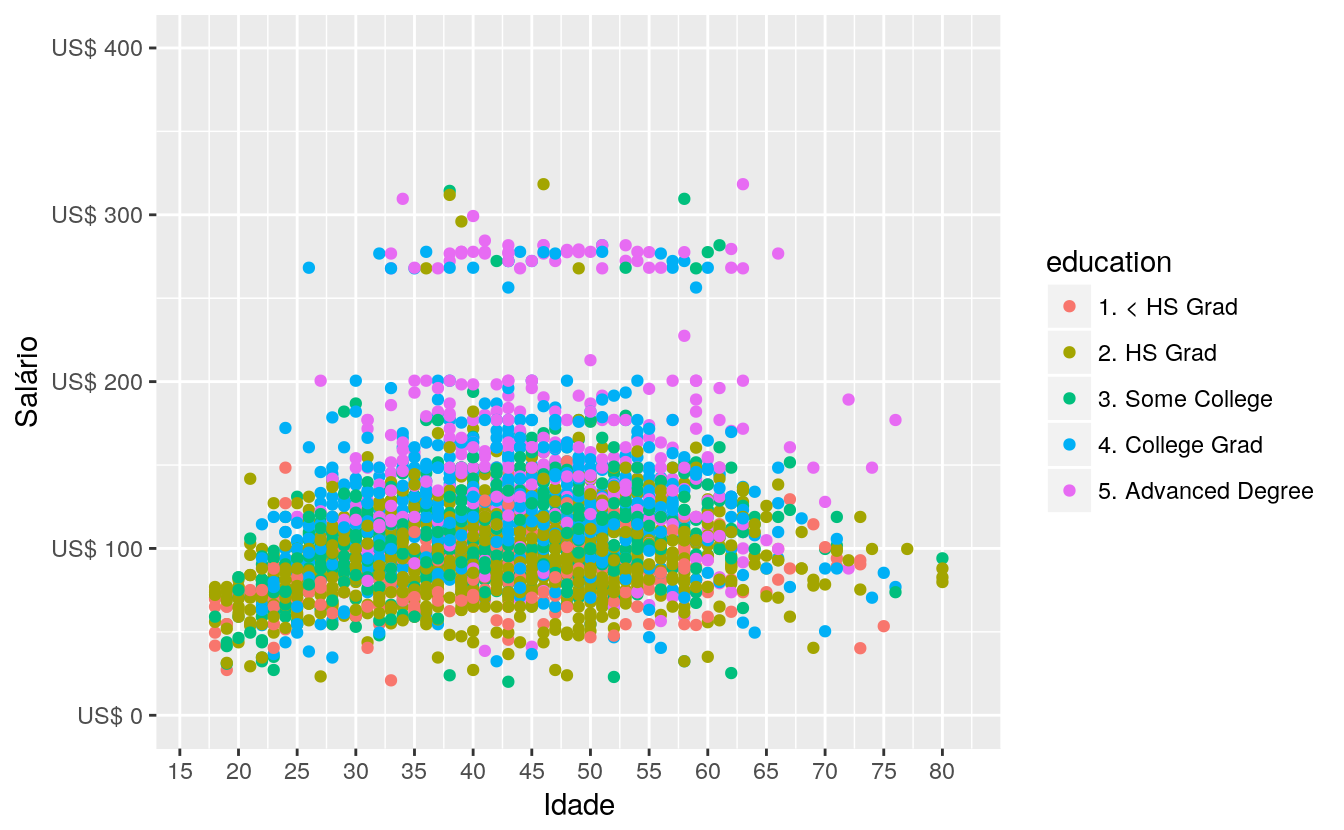
\includegraphics[width=1\linewidth]{bookdown-demo_files/figure-latex/unnamed-chunk-133-1} \end{center}

Para o eixo \texttt{x}, determinamos que as quebras (\texttt{breaks})
acontecem a cada 5 anos. O \texttt{expand(0,0)} é um argumento que
controla os espaços adicionais no final do gráfico. É preciso fornecer
um vetor de tamanho 2, com uma constante multiplicativa e outra aditiva.
No exemplo acima, eliminamos a expansão.

Para o eixo \texttt{y}, informamos que o nome do eixo é
\texttt{Salário}, que os limite inferior e superior são 0 e 400, e
alteramos os rótulos. No caso, passamos uma função que concatena
\texttt{US\$} com o valor que já seria exibido. Note que, sabendo de
antemão todos os breaks, é possível definir manualmente os labels.
Veremos isso no exemplo com variáveis categóricas. No entanto, para
variáveis contínuas, o uso de funções parece mais apropriado.

\subsubsection{Variáveis discretas}\label{variaveis-discretas}

Apesar do \emph{help} não apresentar todos os argumentos para as escalas
discretas, podemos usar quase todos que foram listados para escala
contínua.

\begin{Shaded}
\begin{Highlighting}[]
\KeywordTok{scale_x_discrete}\NormalTok{(..., }\DataTypeTok{expand =} \KeywordTok{waiver}\NormalTok{(), }\DataTypeTok{position =} \StringTok{"bottom"}\NormalTok{)}

\KeywordTok{scale_y_discrete}\NormalTok{(..., }\DataTypeTok{expand =} \KeywordTok{waiver}\NormalTok{(), }\DataTypeTok{position =} \StringTok{"left"}\NormalTok{)}
\end{Highlighting}
\end{Shaded}

No exemplo abaixo, iremos alterar os rótulos para uma escala discreta
que originalmente contém os valores \texttt{Yes} e \texttt{No}.

\begin{Shaded}
\begin{Highlighting}[]
\KeywordTok{ggplot}\NormalTok{(Default, }\KeywordTok{aes}\NormalTok{(}\DataTypeTok{x =}\NormalTok{ default, }\DataTypeTok{y =}\NormalTok{ balance)) }\OperatorTok{+}
\StringTok{  }\KeywordTok{geom_boxplot}\NormalTok{() }\OperatorTok{+}\StringTok{ }
\StringTok{  }\KeywordTok{scale_x_discrete}\NormalTok{(}\StringTok{"Calote"}\NormalTok{, }\DataTypeTok{labels =} \KeywordTok{c}\NormalTok{(}\StringTok{"Não"}\NormalTok{, }\StringTok{"Sim"}\NormalTok{)) }\OperatorTok{+}
\StringTok{  }\KeywordTok{labs}\NormalTok{(}\DataTypeTok{y =} \StringTok{"Valor devido médio após o pagamento mensal"}\NormalTok{)}
\end{Highlighting}
\end{Shaded}

\begin{center}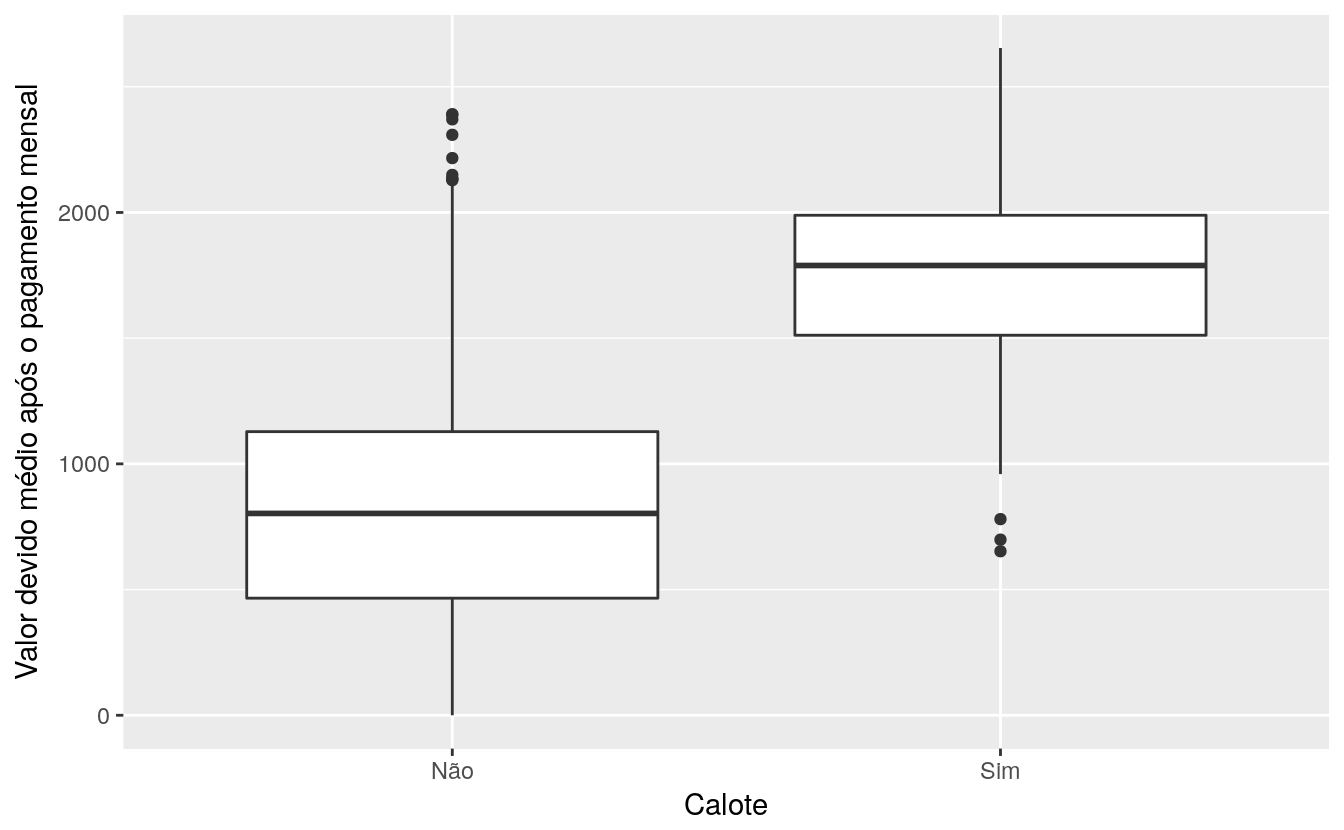
\includegraphics[width=1\linewidth]{bookdown-demo_files/figure-latex/unnamed-chunk-135-1} \end{center}

Pode-se usar o argumento \texttt{limits} para alterar a ordem das
categorias.

\begin{Shaded}
\begin{Highlighting}[]
\KeywordTok{ggplot}\NormalTok{(Default, }\KeywordTok{aes}\NormalTok{(}\DataTypeTok{x =}\NormalTok{ default, }\DataTypeTok{y =}\NormalTok{ balance)) }\OperatorTok{+}
\StringTok{  }\KeywordTok{geom_boxplot}\NormalTok{() }\OperatorTok{+}\StringTok{ }
\StringTok{  }\KeywordTok{scale_x_discrete}\NormalTok{(}\StringTok{"Calote"}\NormalTok{, }\DataTypeTok{limits =} \KeywordTok{c}\NormalTok{(}\StringTok{"Yes"}\NormalTok{, }\StringTok{"No"}\NormalTok{),}
                   \DataTypeTok{labels =} \KeywordTok{c}\NormalTok{(}\StringTok{"Sim"}\NormalTok{, }\StringTok{"Não"}\NormalTok{)) }\OperatorTok{+}
\StringTok{  }\KeywordTok{labs}\NormalTok{(}\DataTypeTok{y =} \StringTok{"Valor devido médio após o pagamento mensal"}\NormalTok{)}
\end{Highlighting}
\end{Shaded}

\begin{center}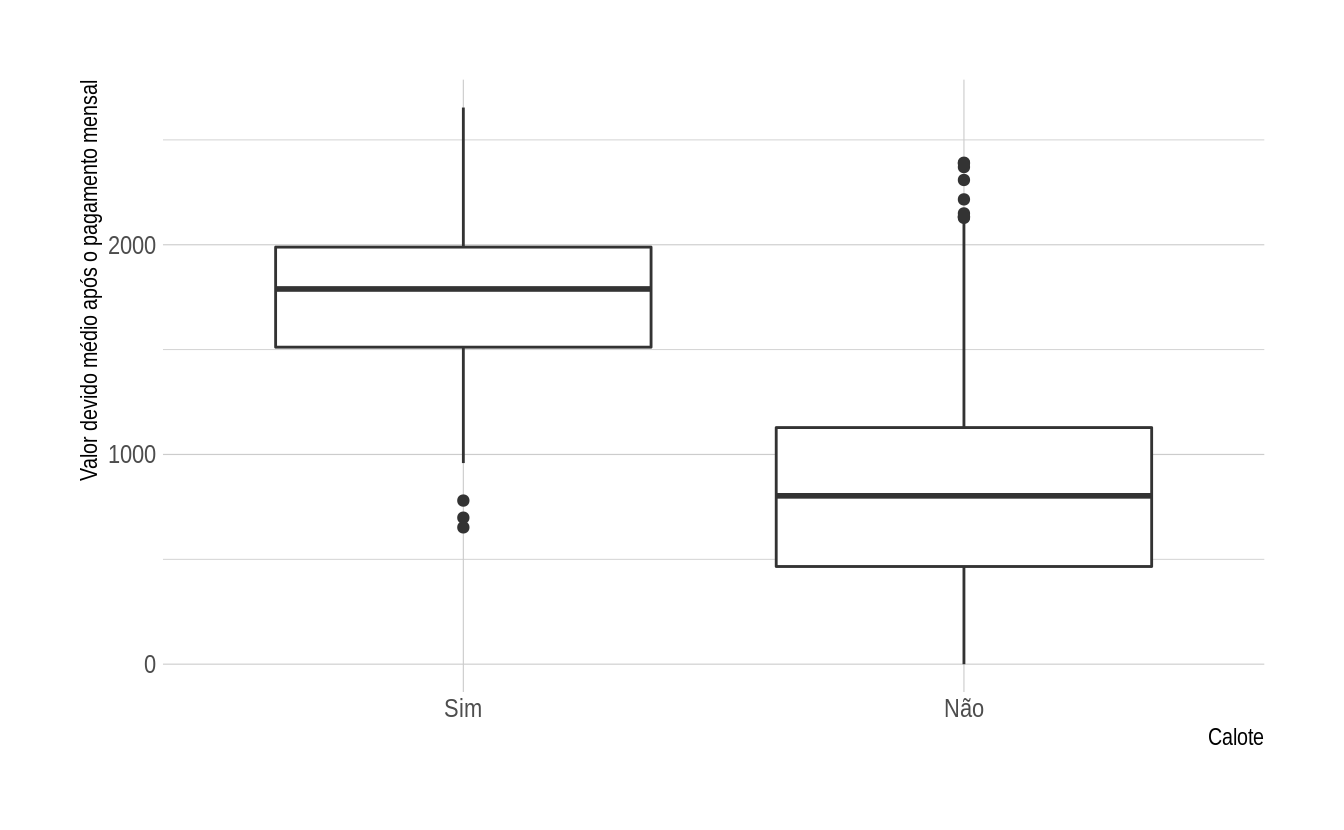
\includegraphics[width=1\linewidth]{bookdown-demo_files/figure-latex/unnamed-chunk-136-1} \end{center}

Também pode-se alterar a ordem de variáveis categóricas alterando a
ordem dos níveis (\texttt{levels}) da variável no data.frame original,
ou usando as funções \texttt{ylim()} e \texttt{xlim()}. Experimente.

\subsubsection{Variáveis de Datas}\label{variaveis-de-datas}

Quando estamos trabalhando com séries temporais é comum que datas sejam
associadas a algum eixo do gŕafico, geralmente ao eixo \texttt{x}. As
funções padrões para controle de escalas dos eixos para variáveis de
datas são as seguintes:

\begin{Shaded}
\begin{Highlighting}[]
\KeywordTok{scale_x_date}\NormalTok{(}\DataTypeTok{name =} \KeywordTok{waiver}\NormalTok{(), }\DataTypeTok{breaks =} \KeywordTok{waiver}\NormalTok{(), }\DataTypeTok{date_breaks =} \KeywordTok{waiver}\NormalTok{(),}
             \DataTypeTok{labels =} \KeywordTok{waiver}\NormalTok{(), }\DataTypeTok{date_labels =} \KeywordTok{waiver}\NormalTok{(), }\DataTypeTok{minor_breaks =} \KeywordTok{waiver}\NormalTok{(),}
             \DataTypeTok{date_minor_breaks =} \KeywordTok{waiver}\NormalTok{(), }\DataTypeTok{limits =} \OtherTok{NULL}\NormalTok{, }\DataTypeTok{expand =} \KeywordTok{waiver}\NormalTok{())}

\KeywordTok{scale_y_date}\NormalTok{(}\DataTypeTok{name =} \KeywordTok{waiver}\NormalTok{(), }\DataTypeTok{breaks =} \KeywordTok{waiver}\NormalTok{(), }\DataTypeTok{date_breaks =} \KeywordTok{waiver}\NormalTok{(),}
             \DataTypeTok{labels =} \KeywordTok{waiver}\NormalTok{(), }\DataTypeTok{date_labels =} \KeywordTok{waiver}\NormalTok{(), }\DataTypeTok{minor_breaks =} \KeywordTok{waiver}\NormalTok{(),}
             \DataTypeTok{date_minor_breaks =} \KeywordTok{waiver}\NormalTok{(), }\DataTypeTok{limits =} \OtherTok{NULL}\NormalTok{, }\DataTypeTok{expand =} \KeywordTok{waiver}\NormalTok{())}

\KeywordTok{scale_x_datetime}\NormalTok{(}\DataTypeTok{name =} \KeywordTok{waiver}\NormalTok{(), }\DataTypeTok{breaks =} \KeywordTok{waiver}\NormalTok{(), }\DataTypeTok{date_breaks =} \KeywordTok{waiver}\NormalTok{(),}
                 \DataTypeTok{labels =} \KeywordTok{waiver}\NormalTok{(), }\DataTypeTok{date_labels =} \KeywordTok{waiver}\NormalTok{(), }\DataTypeTok{minor_breaks =} \KeywordTok{waiver}\NormalTok{(),}
                 \DataTypeTok{date_minor_breaks =} \KeywordTok{waiver}\NormalTok{(), }\DataTypeTok{limits =} \OtherTok{NULL}\NormalTok{, }\DataTypeTok{expand =} \KeywordTok{waiver}\NormalTok{())}

\KeywordTok{scale_y_datetime}\NormalTok{(}\DataTypeTok{name =} \KeywordTok{waiver}\NormalTok{(), }\DataTypeTok{breaks =} \KeywordTok{waiver}\NormalTok{(), }\DataTypeTok{date_breaks =} \KeywordTok{waiver}\NormalTok{(),}
                 \DataTypeTok{labels =} \KeywordTok{waiver}\NormalTok{(), }\DataTypeTok{date_labels =} \KeywordTok{waiver}\NormalTok{(), }\DataTypeTok{minor_breaks =} \KeywordTok{waiver}\NormalTok{(),}
                 \DataTypeTok{date_minor_breaks =} \KeywordTok{waiver}\NormalTok{(), }\DataTypeTok{limits =} \OtherTok{NULL}\NormalTok{, }\DataTypeTok{expand =} \KeywordTok{waiver}\NormalTok{())}
\end{Highlighting}
\end{Shaded}

\texttt{scale\_*\_date} é utilizado para variáveis do tipo \texttt{Date}
e \texttt{scale\_*\_datetime} para variáveis do tipo \texttt{POSIXct}. A
classe \texttt{POSIXct} aceita informações relacionados a tempo/horário
e a classe \texttt{Date} aceita apenas dia, mês e ano.

O mais importante é a possibilidade de alterar como as datas são
apresentadas a partir do argumento \texttt{date\_labels}. Para isso,
vamos utilizar um exemplo a partir dos dados \texttt{economics}.
Primeiro, observa-se o resultado padrão do ggplot2:

\begin{Shaded}
\begin{Highlighting}[]
\KeywordTok{ggplot}\NormalTok{(economics, }\KeywordTok{aes}\NormalTok{(}\DataTypeTok{x =}\NormalTok{ date, }\DataTypeTok{y =}\NormalTok{ unemploy)) }\OperatorTok{+}
\StringTok{  }\KeywordTok{geom_line}\NormalTok{() }
\end{Highlighting}
\end{Shaded}

\begin{center}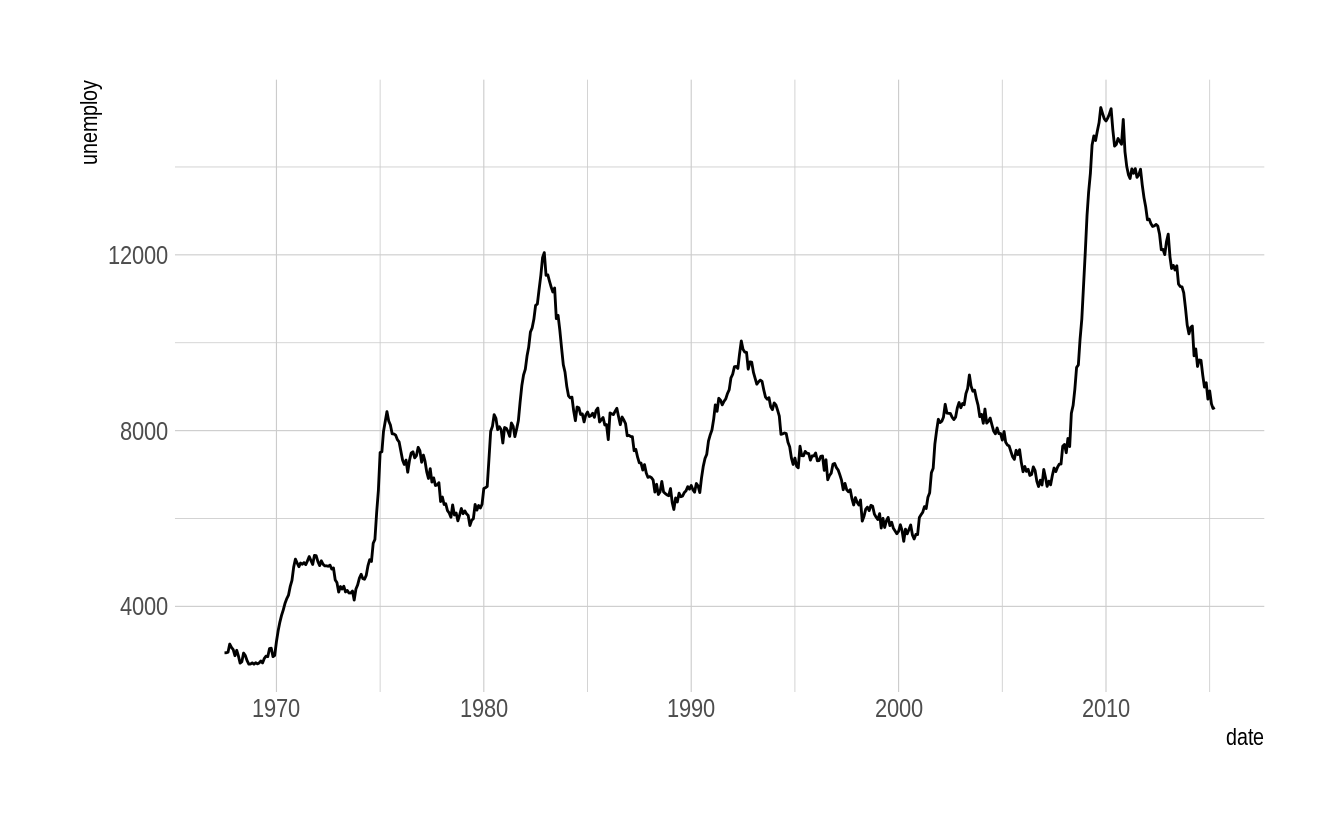
\includegraphics[width=1\linewidth]{bookdown-demo_files/figure-latex/unnamed-chunk-139-1} \end{center}

Agora, suponha que queremos alterar o gráfico para o formato
``Jan/1970'':

\begin{Shaded}
\begin{Highlighting}[]
\KeywordTok{ggplot}\NormalTok{(economics, }\KeywordTok{aes}\NormalTok{(}\DataTypeTok{x =}\NormalTok{ date, }\DataTypeTok{y =}\NormalTok{ unemploy)) }\OperatorTok{+}
\StringTok{  }\KeywordTok{geom_line}\NormalTok{() }\OperatorTok{+}
\StringTok{  }\KeywordTok{scale_x_date}\NormalTok{(}\DataTypeTok{date_labels =} \StringTok{"%b/%Y"}\NormalTok{)}
\end{Highlighting}
\end{Shaded}

\begin{center}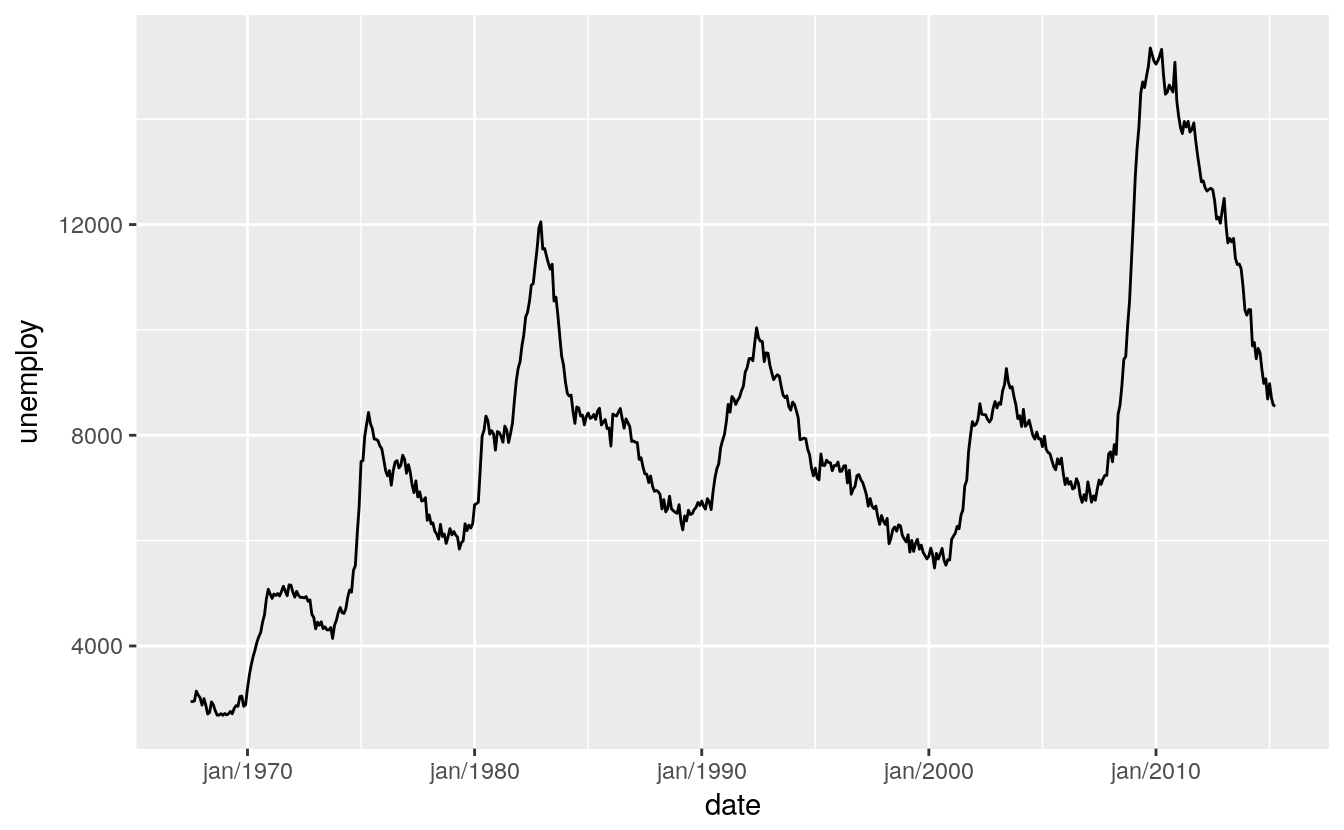
\includegraphics[width=1\linewidth]{bookdown-demo_files/figure-latex/unnamed-chunk-140-1} \end{center}

O uso do \texttt{\%b/\%Y} é usado para definir o formato de data
desejado. Para ver a lista de formatos, use \texttt{help(strptime)}.
Para os \texttt{breaks}, temos duas opções. A primeira é utilizar o
argumento \texttt{breaks} informando um vetor de datas ou usando o
argumento \texttt{date\_breaks}, em que se informa a frequência dos
breaks (por exemplo, ``1 month'' e ``5 years''). Veja os exemplos
abaixos:

\begin{Shaded}
\begin{Highlighting}[]
\KeywordTok{ggplot}\NormalTok{(economics, }\KeywordTok{aes}\NormalTok{(}\DataTypeTok{x =}\NormalTok{ date, }\DataTypeTok{y =}\NormalTok{ unemploy)) }\OperatorTok{+}
\StringTok{  }\KeywordTok{geom_line}\NormalTok{() }\OperatorTok{+}
\StringTok{  }\KeywordTok{scale_x_date}\NormalTok{(}\DataTypeTok{date_breaks =} \StringTok{"5 years"}\NormalTok{, }\DataTypeTok{date_labels =} \StringTok{"%Y"}\NormalTok{)}
\end{Highlighting}
\end{Shaded}

\begin{center}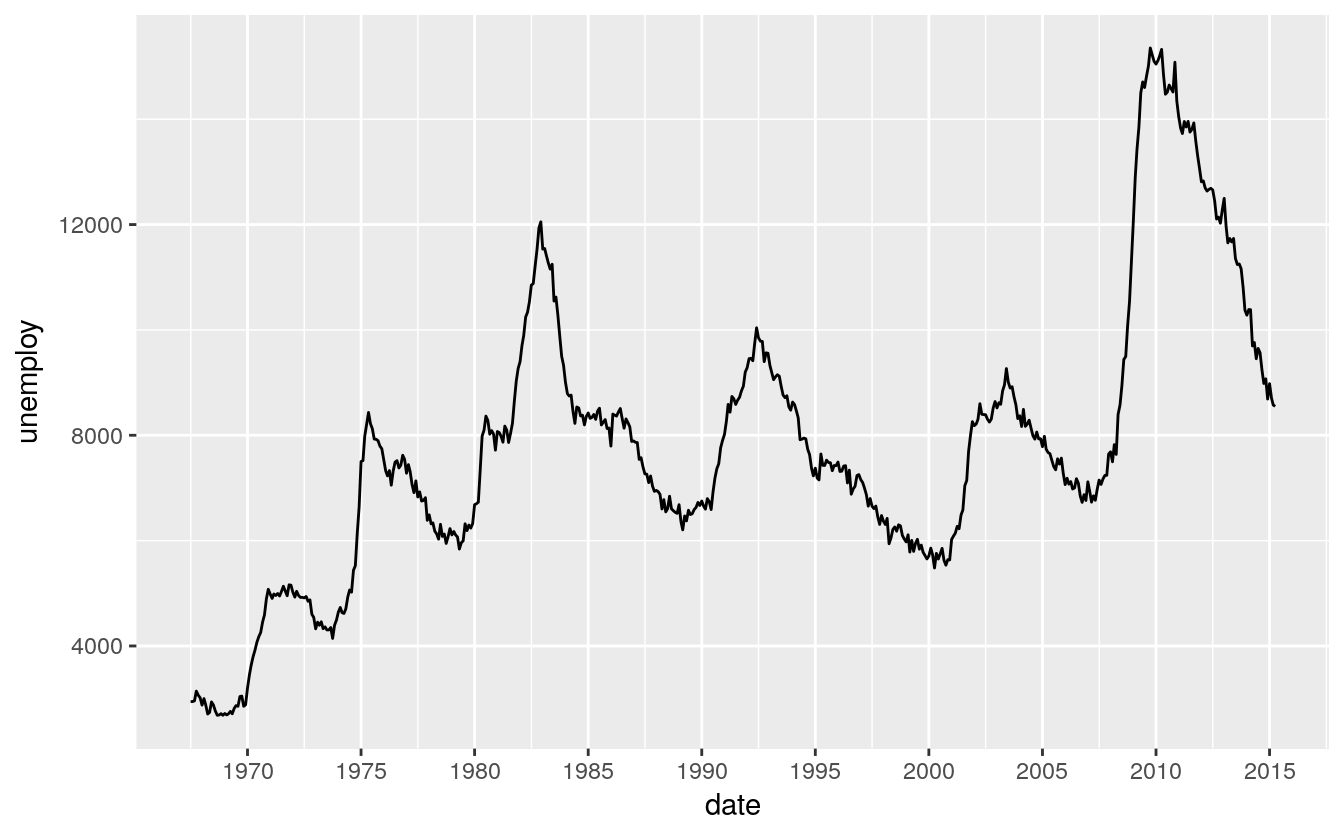
\includegraphics[width=1\linewidth]{bookdown-demo_files/figure-latex/unnamed-chunk-141-1} \end{center}

\begin{Shaded}
\begin{Highlighting}[]
\NormalTok{seq_datas <-}\StringTok{ }\KeywordTok{seq.Date}\NormalTok{(}\KeywordTok{as.Date}\NormalTok{(}\StringTok{'1970-01-01'}\NormalTok{),}
                      \KeywordTok{as.Date}\NormalTok{(}\StringTok{'2015-04-01'}\NormalTok{),}
                      \DataTypeTok{by =} \StringTok{'5 years'}\NormalTok{)}
\KeywordTok{ggplot}\NormalTok{(economics, }\KeywordTok{aes}\NormalTok{(}\DataTypeTok{x =}\NormalTok{ date, }\DataTypeTok{y =}\NormalTok{ unemploy)) }\OperatorTok{+}
\StringTok{  }\KeywordTok{geom_line}\NormalTok{() }\OperatorTok{+}
\StringTok{  }\KeywordTok{scale_x_date}\NormalTok{(}\DataTypeTok{breaks =}\NormalTok{ seq_datas, }\DataTypeTok{date_labels =} \StringTok{"%Y"}\NormalTok{)}
\end{Highlighting}
\end{Shaded}

\begin{center}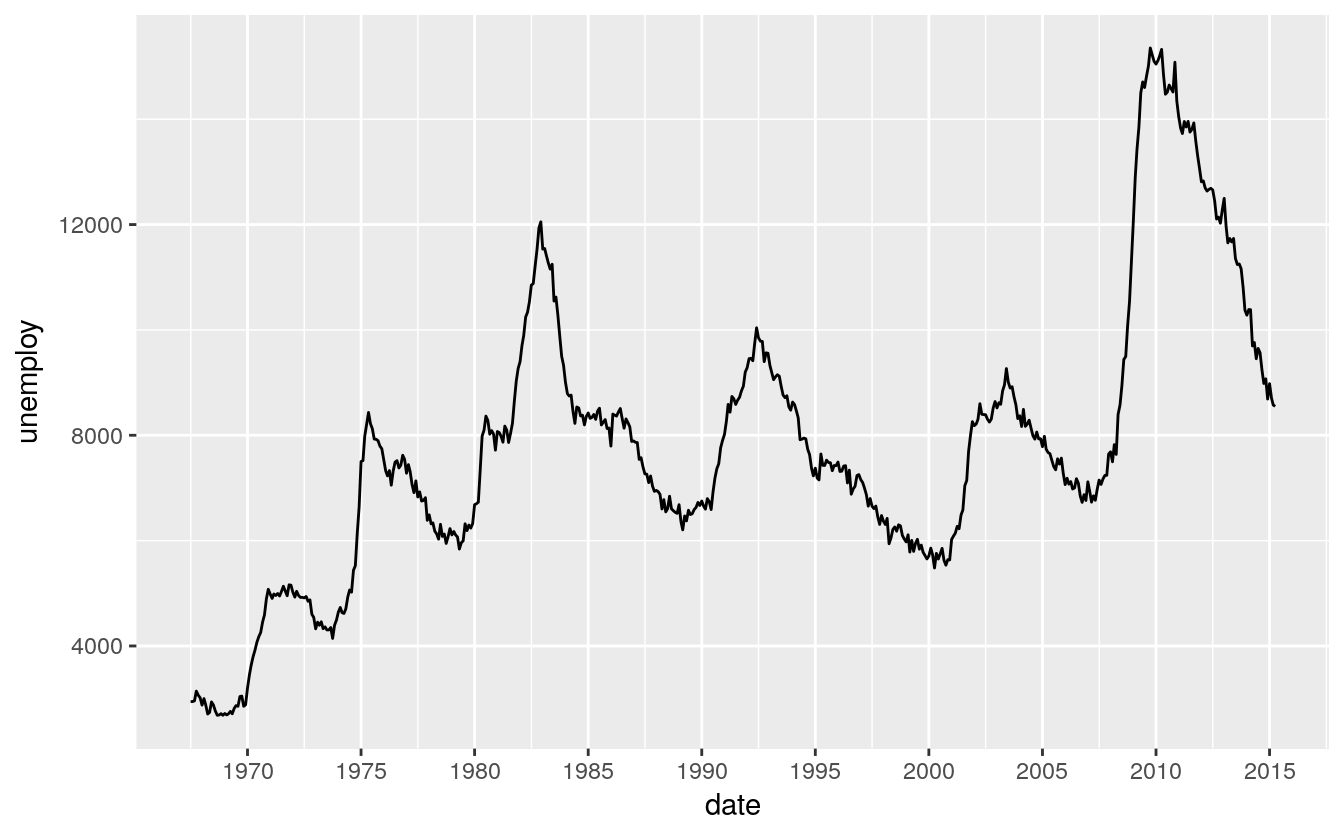
\includegraphics[width=1\linewidth]{bookdown-demo_files/figure-latex/unnamed-chunk-142-1} \end{center}

\subsection{Escalas de Cores (color) e Preenchimento
(fill)}\label{escalas-de-cores-color-e-preenchimento-fill}

Como nos casos dos eixos \texttt{x} e \texttt{y}, o tipo da variável
utilizada define qual o tipo de escala.

\begin{longtable}[]{@{}lll@{}}
\toprule
\begin{minipage}[b]{0.12\columnwidth}\raggedright\strut
Tipo da Variável\strut
\end{minipage} & \begin{minipage}[b]{0.11\columnwidth}\raggedright\strut
Escala\strut
\end{minipage} & \begin{minipage}[b]{0.68\columnwidth}\raggedright\strut
Descrição\strut
\end{minipage}\tabularnewline
\midrule
\endhead
\begin{minipage}[t]{0.12\columnwidth}\raggedright\strut
Discreta\strut
\end{minipage} & \begin{minipage}[t]{0.11\columnwidth}\raggedright\strut
\textbf{hue}\strut
\end{minipage} & \begin{minipage}[t]{0.68\columnwidth}\raggedright\strut
escolhe n cores igualmente espaçadas em um disco de cores. É possível
editar a luminosidade e a saturação.\strut
\end{minipage}\tabularnewline
\begin{minipage}[t]{0.12\columnwidth}\raggedright\strut
\strut
\end{minipage} & \begin{minipage}[t]{0.11\columnwidth}\raggedright\strut
grey\strut
\end{minipage} & \begin{minipage}[t]{0.68\columnwidth}\raggedright\strut
escala de cinza\strut
\end{minipage}\tabularnewline
\begin{minipage}[t]{0.12\columnwidth}\raggedright\strut
\strut
\end{minipage} & \begin{minipage}[t]{0.11\columnwidth}\raggedright\strut
brewer\strut
\end{minipage} & \begin{minipage}[t]{0.68\columnwidth}\raggedright\strut
ver pacote RColorBrewer\strut
\end{minipage}\tabularnewline
\begin{minipage}[t]{0.12\columnwidth}\raggedright\strut
\strut
\end{minipage} & \begin{minipage}[t]{0.11\columnwidth}\raggedright\strut
identity\strut
\end{minipage} & \begin{minipage}[t]{0.68\columnwidth}\raggedright\strut
usa as cores inseridas na própria variável\strut
\end{minipage}\tabularnewline
\begin{minipage}[t]{0.12\columnwidth}\raggedright\strut
\strut
\end{minipage} & \begin{minipage}[t]{0.11\columnwidth}\raggedright\strut
manual\strut
\end{minipage} & \begin{minipage}[t]{0.68\columnwidth}\raggedright\strut
escolher as cores manualmente\strut
\end{minipage}\tabularnewline
\begin{minipage}[t]{0.12\columnwidth}\raggedright\strut
Contínua\strut
\end{minipage} & \begin{minipage}[t]{0.11\columnwidth}\raggedright\strut
\textbf{gradient}\strut
\end{minipage} & \begin{minipage}[t]{0.68\columnwidth}\raggedright\strut
cria um gradiente de duas cores (low-high)\strut
\end{minipage}\tabularnewline
\begin{minipage}[t]{0.12\columnwidth}\raggedright\strut
\strut
\end{minipage} & \begin{minipage}[t]{0.11\columnwidth}\raggedright\strut
gradient2\strut
\end{minipage} & \begin{minipage}[t]{0.68\columnwidth}\raggedright\strut
cria um gradiente de cores divergentes (low-mid-high)\strut
\end{minipage}\tabularnewline
\begin{minipage}[t]{0.12\columnwidth}\raggedright\strut
\strut
\end{minipage} & \begin{minipage}[t]{0.11\columnwidth}\raggedright\strut
gradientn\strut
\end{minipage} & \begin{minipage}[t]{0.68\columnwidth}\raggedright\strut
cria um gradiente com n cores\strut
\end{minipage}\tabularnewline
\bottomrule
\end{longtable}

A opção \texttt{hue} usa a seguinte roda de cores:

\begin{figure}

{\centering 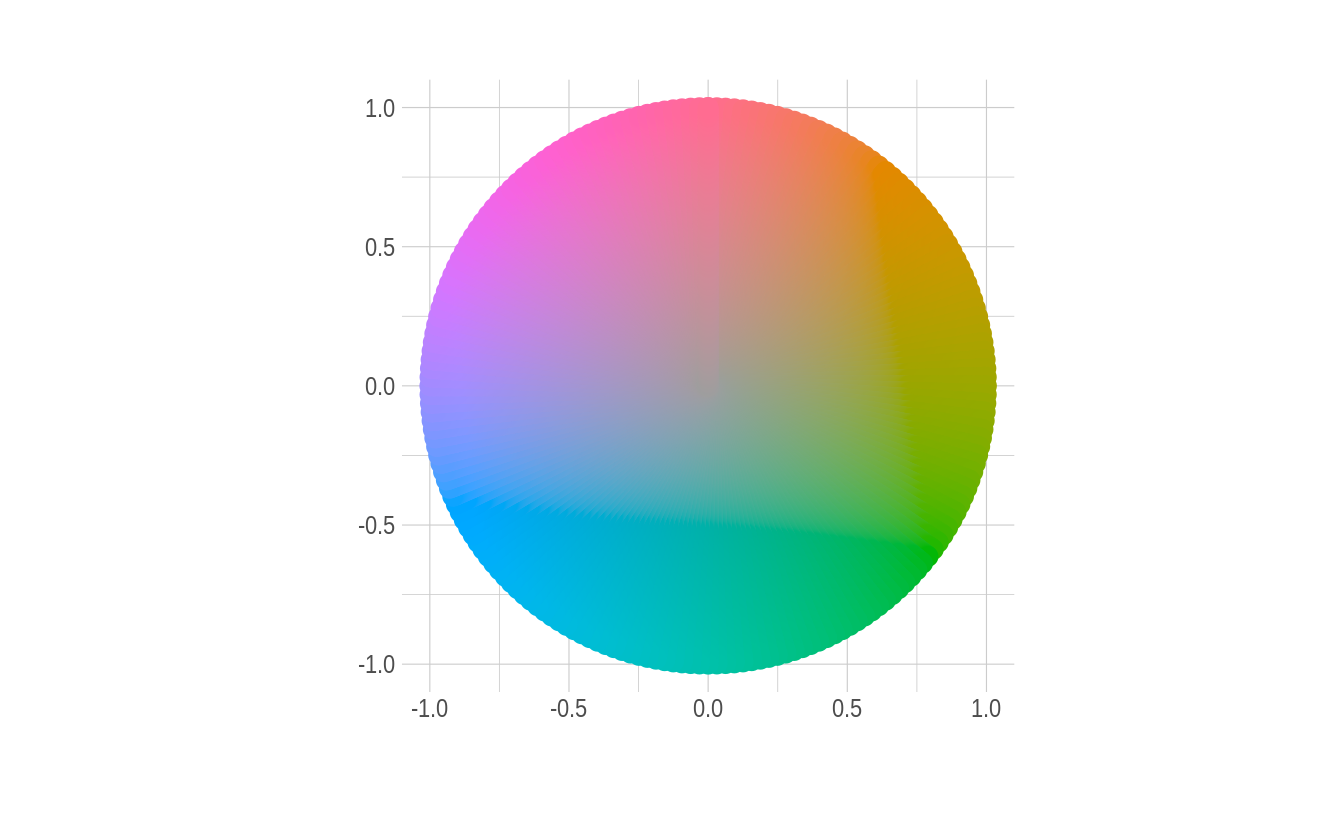
\includegraphics[width=1\linewidth]{bookdown-demo_files/figure-latex/unnamed-chunk-143-1} 

}

\caption{Roda de Cores - hue}\label{fig:unnamed-chunk-143}
\end{figure}

A opção brewer pode usar as paletas de cores disponíveis no pacote
RColorBrewer.

\begin{Shaded}
\begin{Highlighting}[]
\KeywordTok{library}\NormalTok{(RColorBrewer)}
\KeywordTok{display.brewer.all}\NormalTok{(}\DataTypeTok{n=}\OtherTok{NULL}\NormalTok{, }\DataTypeTok{type=}\StringTok{"all"}\NormalTok{, }\DataTypeTok{select=}\OtherTok{NULL}\NormalTok{, }\DataTypeTok{exact.n=}\OtherTok{TRUE}\NormalTok{,}
                                 \DataTypeTok{colorblindFriendly=}\OtherTok{FALSE}\NormalTok{)}
\end{Highlighting}
\end{Shaded}

\begin{center}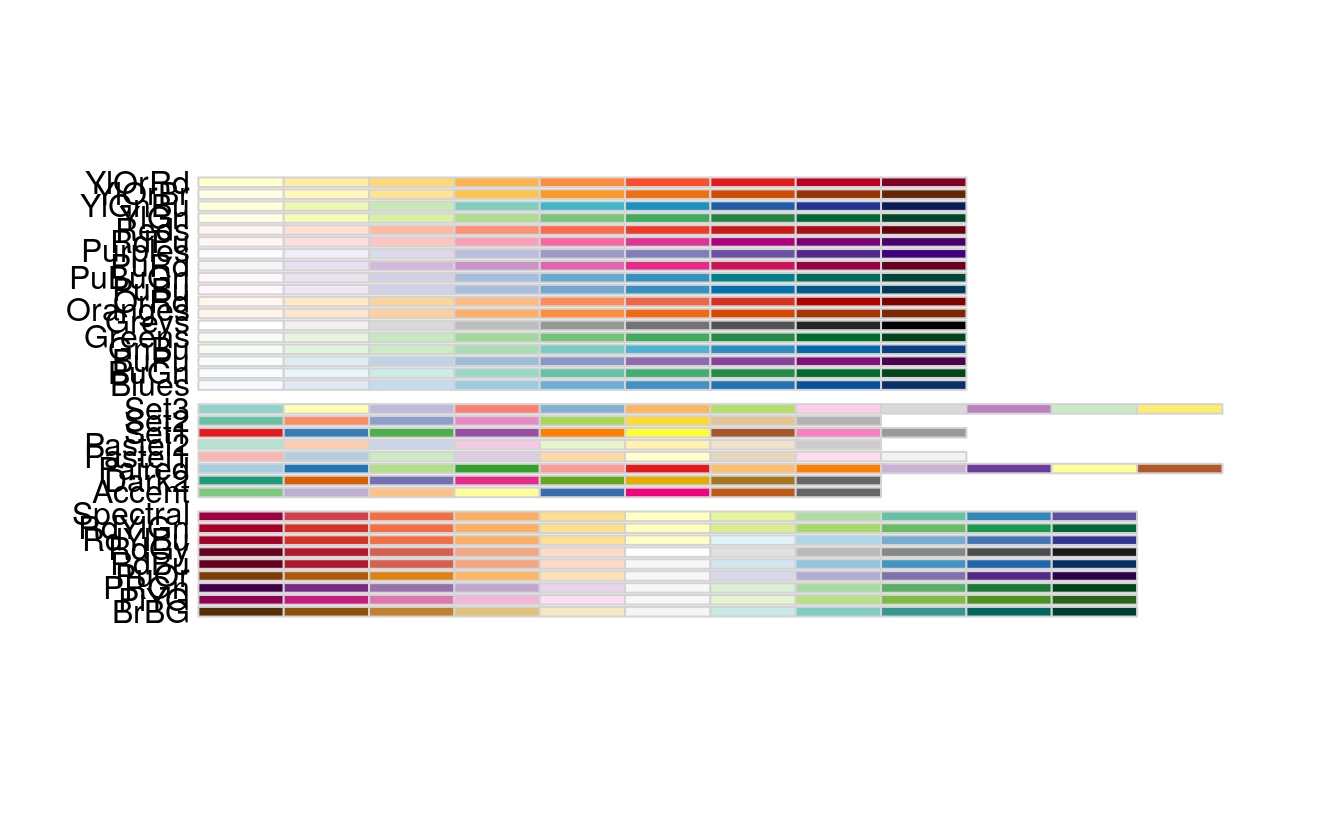
\includegraphics[width=1\linewidth]{bookdown-demo_files/figure-latex/unnamed-chunk-144-1} \end{center}

No exemplo abaixo, vamos utilizar a função \texttt{brewer.pal} que
retorna um vetor de cores de alguma paleta do pacote RColorBrewer. O
objeto \texttt{paleta.gradientn} recebe 9 cores da paleta \texttt{Reds}.
Essas cores são utilizadas na função \texttt{scale\_fill\_gradientn()}.

\begin{Shaded}
\begin{Highlighting}[]
\NormalTok{paleta.gradientn <-}\StringTok{ }\KeywordTok{brewer.pal}\NormalTok{(}\DataTypeTok{n =} \DecValTok{10}\NormalTok{, }\DataTypeTok{name =} \StringTok{'Reds'}\NormalTok{)}
\end{Highlighting}
\end{Shaded}

\begin{verbatim}
## Warning in brewer.pal(n = 10, name = "Reds"): n too large, allowed maximum for palette Reds is 9
## Returning the palette you asked for with that many colors
\end{verbatim}

\begin{Shaded}
\begin{Highlighting}[]
\NormalTok{Credit }\OperatorTok\StringTok{ }
\StringTok{  }\KeywordTok{group_by}\NormalTok{(Cards, Student) }\OperatorTok
\StringTok{  }\KeywordTok{summarise}\NormalTok{(}\DataTypeTok{Balance =} \KeywordTok{mean}\NormalTok{(Balance), }\DataTypeTok{n =} \KeywordTok{n}\NormalTok{()) }\OperatorTok\StringTok{ }
\StringTok{  }\KeywordTok{ggplot}\NormalTok{(}\KeywordTok{aes}\NormalTok{(}\DataTypeTok{x =}\NormalTok{ Cards, }\DataTypeTok{y =}\NormalTok{ Student, }\DataTypeTok{fill =}\NormalTok{ Balance)) }\OperatorTok{+}
\StringTok{  }\KeywordTok{geom_tile}\NormalTok{() }\OperatorTok{+}
\StringTok{  }\KeywordTok{scale_fill_gradientn}\NormalTok{(}\DataTypeTok{colors =} \KeywordTok{rev}\NormalTok{(paleta.gradientn)) }\OperatorTok{+}
\StringTok{  }\KeywordTok{scale_x_continuous}\NormalTok{(}\DataTypeTok{breaks =} \DecValTok{1}\OperatorTok{:}\DecValTok{9}\NormalTok{)}
\end{Highlighting}
\end{Shaded}

\begin{center}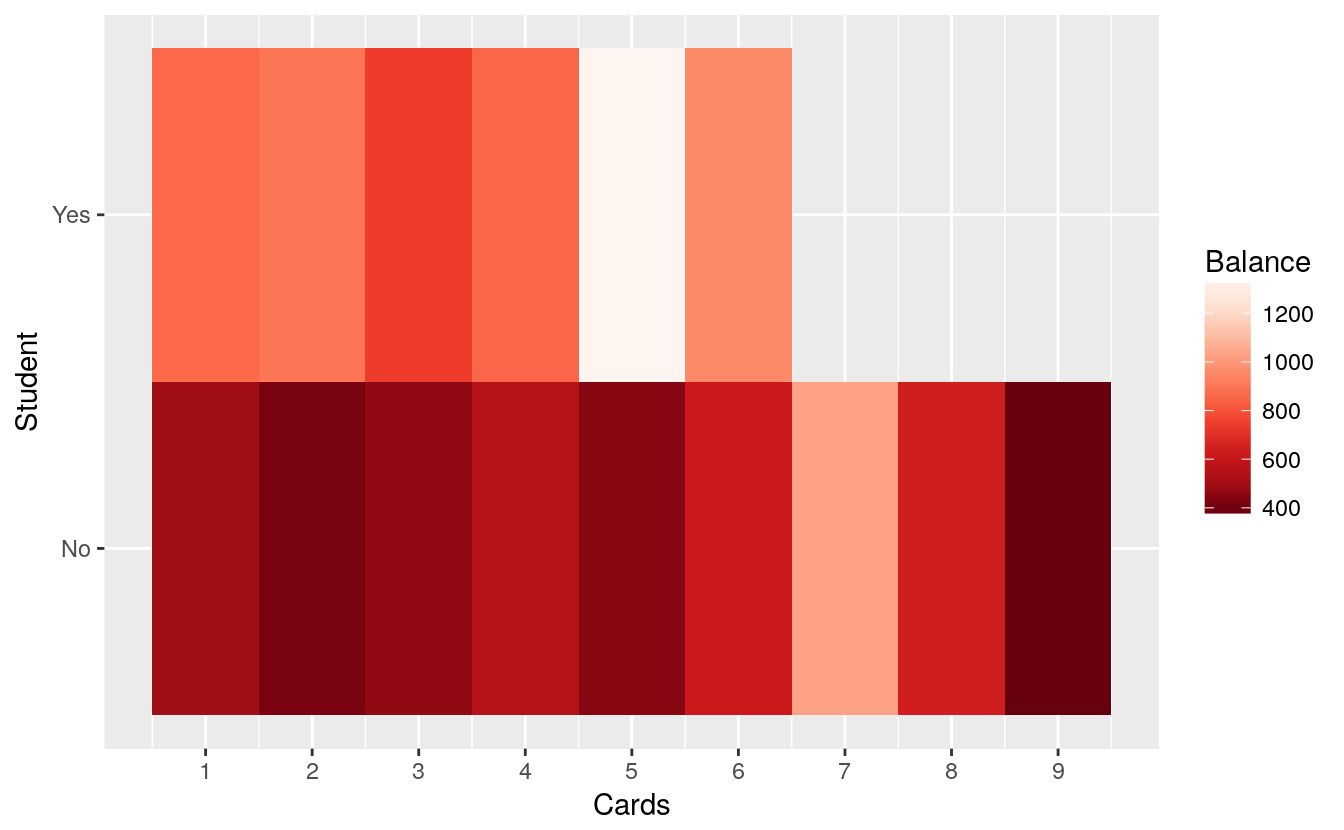
\includegraphics[width=1\linewidth]{bookdown-demo_files/figure-latex/unnamed-chunk-145-1} \end{center}

Alguns pacotes também fornecem escalas de cores próprias, como é o caso
do pacote \texttt{viridis}.

\begin{Shaded}
\begin{Highlighting}[]
\NormalTok{Credit }\OperatorTok\StringTok{ }
\StringTok{  }\KeywordTok{group_by}\NormalTok{(Cards, Student) }\OperatorTok
\StringTok{  }\KeywordTok{summarise}\NormalTok{(}\DataTypeTok{Balance =} \KeywordTok{mean}\NormalTok{(Balance), }\DataTypeTok{n =} \KeywordTok{n}\NormalTok{()) }\OperatorTok\StringTok{ }
\StringTok{  }\KeywordTok{ggplot}\NormalTok{(}\KeywordTok{aes}\NormalTok{(}\DataTypeTok{x =}\NormalTok{ Cards, }\DataTypeTok{y =}\NormalTok{ Student, }\DataTypeTok{fill =}\NormalTok{ Balance)) }\OperatorTok{+}
\StringTok{  }\KeywordTok{geom_tile}\NormalTok{() }\OperatorTok{+}
\StringTok{  }\NormalTok{viridis}\OperatorTok{::}\KeywordTok{scale_fill_viridis}\NormalTok{() }\OperatorTok{+}
\StringTok{  }\KeywordTok{scale_x_continuous}\NormalTok{(}\DataTypeTok{breaks =} \DecValTok{1}\OperatorTok{:}\DecValTok{9}\NormalTok{)}
\end{Highlighting}
\end{Shaded}

\begin{center}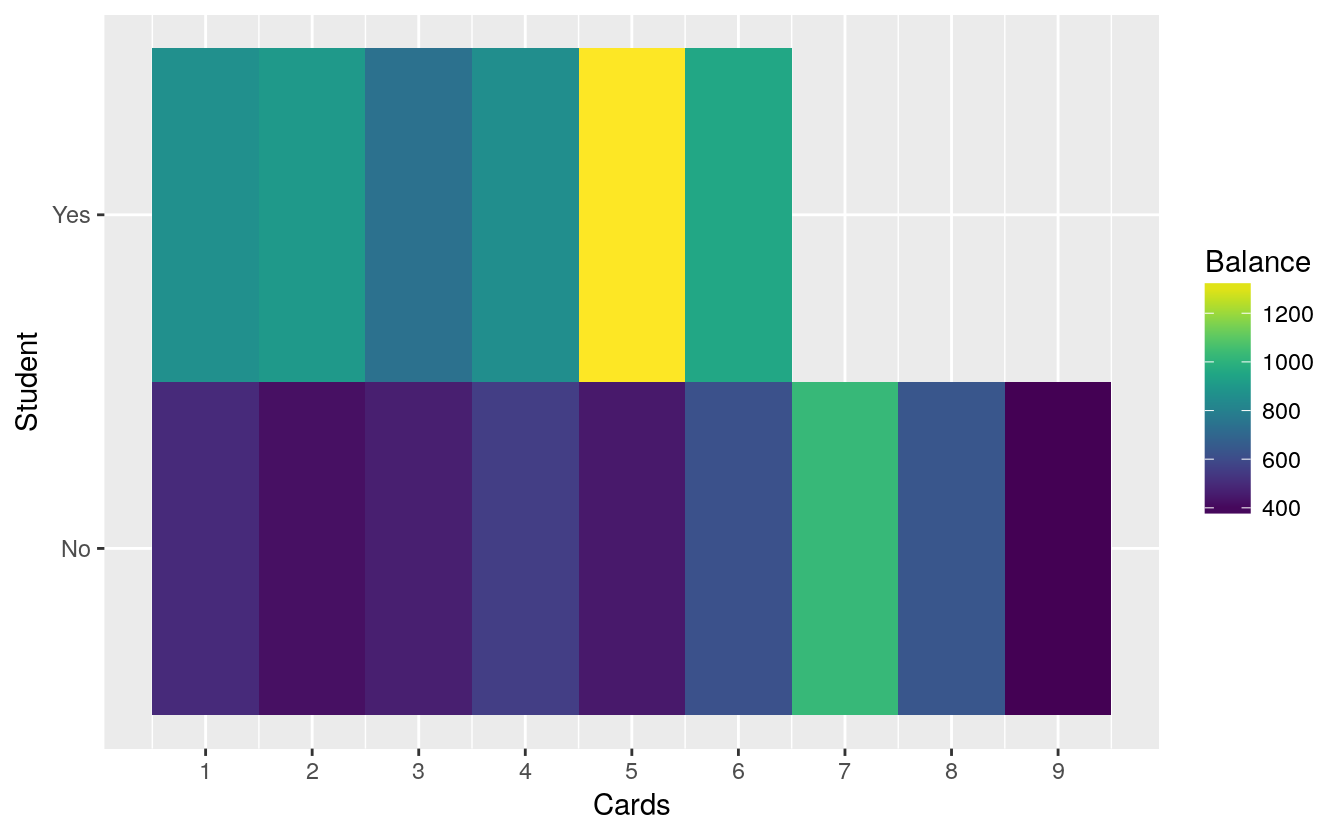
\includegraphics[width=1\linewidth]{bookdown-demo_files/figure-latex/unnamed-chunk-146-1} \end{center}

Agora, vamos fazer um exemplo usando o \texttt{scale\_color\_manual()}.

\begin{Shaded}
\begin{Highlighting}[]
\KeywordTok{ggplot}\NormalTok{(Wage, }\KeywordTok{aes}\NormalTok{(}\DataTypeTok{y =}\NormalTok{ wage, }\DataTypeTok{x =}\NormalTok{ age, }\DataTypeTok{color =}\NormalTok{ education)) }\OperatorTok{+}
\StringTok{  }\KeywordTok{geom_point}\NormalTok{() }\OperatorTok{+}
\StringTok{  }\KeywordTok{scale_color_manual}\NormalTok{(}\DataTypeTok{values =} \KeywordTok{c}\NormalTok{(}\StringTok{"#66C2A5"}\NormalTok{, }\StringTok{"#FC8D62"}\NormalTok{, }\StringTok{"#8DA0CB"}\NormalTok{, }\StringTok{"#E78AC3"}\NormalTok{, }\StringTok{"#A6D854"}\NormalTok{))}
\end{Highlighting}
\end{Shaded}

\begin{center}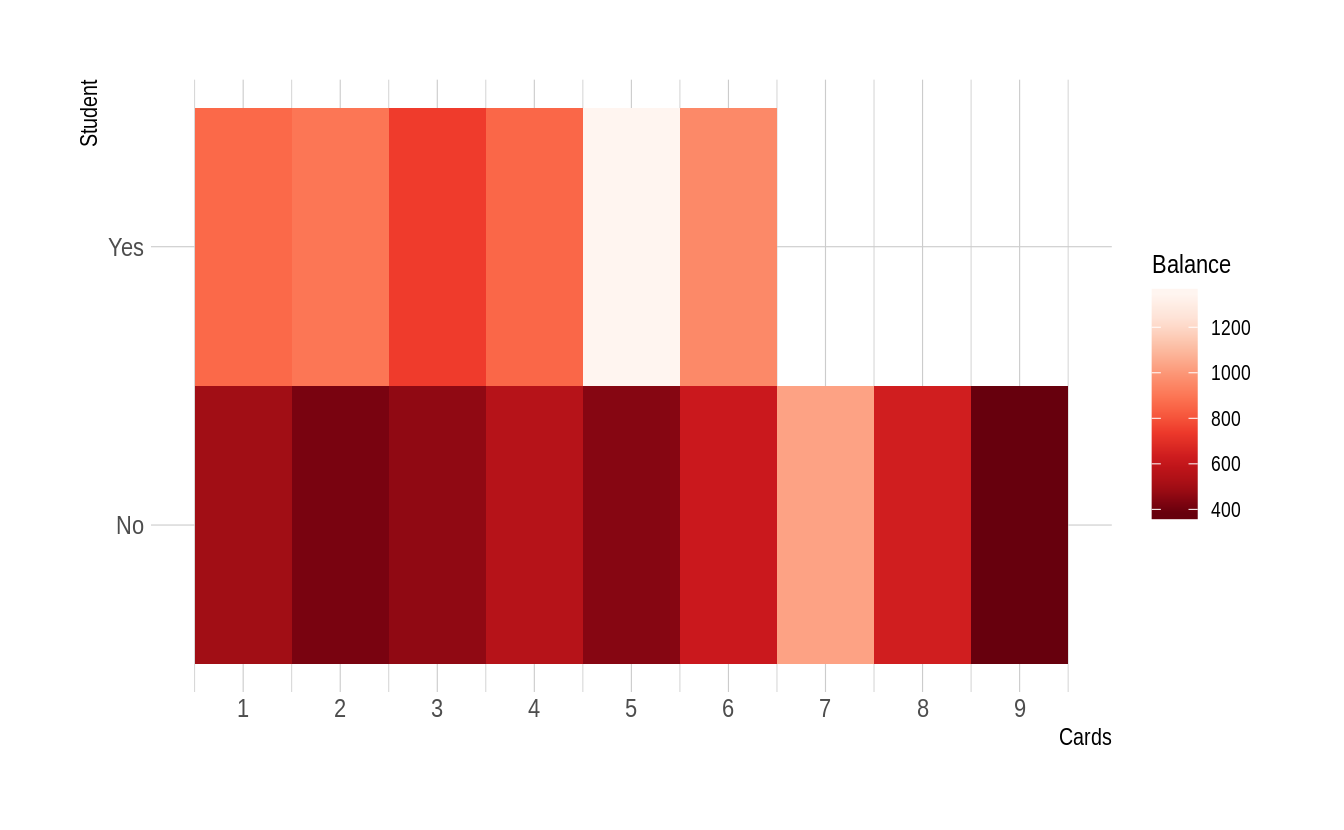
\includegraphics[width=1\linewidth]{bookdown-demo_files/figure-latex/unnamed-chunk-147-1} \end{center}

Aqui fizemos uma introdução ao componente de escalas. Não tratamos de
todas as funções de escalas. A ideia é passar a lógica geral para se
utilizar escalas, e não que o usuário decore todas as funções, o que
contraproducente.

\section{Subplots (facet)}\label{subplots-facet}

O ggplot2 facilita a criação de subplots no caso em que se deseja
replicar o mesmo gráfico para um conjunto de valores de outra variável.
Por exemplo, criar um gráfico da série temporal de desemprego para cada
Unidade da Federação. As duas principais funções são
\texttt{facet\_wrap()} e \texttt{facet\_grid()}.

\begin{itemize}
\tightlist
\item
  Painéis em formato de grid:
\end{itemize}

\begin{Shaded}
\begin{Highlighting}[]
\KeywordTok{facet_grid}\NormalTok{(facets, }\DataTypeTok{margins =} \OtherTok{FALSE}\NormalTok{, }\DataTypeTok{scales =} \StringTok{"fixed"}\NormalTok{, }\DataTypeTok{space =} \StringTok{"fixed"}\NormalTok{, }\DataTypeTok{shrink =} \OtherTok{TRUE}\NormalTok{,}
           \DataTypeTok{labeller =} \StringTok{"label_value"}\NormalTok{, }\DataTypeTok{as.table =} \OtherTok{TRUE}\NormalTok{, }\DataTypeTok{switch =} \OtherTok{NULL}\NormalTok{, }\DataTypeTok{drop =} \OtherTok{TRUE}\NormalTok{)}
\end{Highlighting}
\end{Shaded}

\begin{itemize}
\tightlist
\item
  Converte painéis de uma dimensão para duas dimensões:
\end{itemize}

\begin{Shaded}
\begin{Highlighting}[]
\KeywordTok{facet_wrap}\NormalTok{(facets, }\DataTypeTok{nrow =} \OtherTok{NULL}\NormalTok{, }\DataTypeTok{ncol =} \OtherTok{NULL}\NormalTok{, }\DataTypeTok{scales =} \StringTok{"fixed"}\NormalTok{, }\DataTypeTok{shrink =} \OtherTok{TRUE}\NormalTok{,}
           \DataTypeTok{labeller =} \StringTok{"label_value"}\NormalTok{, }\DataTypeTok{as.table =} \OtherTok{TRUE}\NormalTok{, }\DataTypeTok{switch =} \OtherTok{NULL}\NormalTok{, }\DataTypeTok{drop =} \OtherTok{TRUE}\NormalTok{,}
           \DataTypeTok{dir =} \StringTok{"h"}\NormalTok{)}
\end{Highlighting}
\end{Shaded}

Primeiramente, vamos criar um exemplo para o \texttt{facet\_wrap()}:

\begin{Shaded}
\begin{Highlighting}[]
\KeywordTok{ggplot}\NormalTok{(diamonds, }\KeywordTok{aes}\NormalTok{(}\DataTypeTok{x =}\NormalTok{ carat, }\DataTypeTok{y =}\NormalTok{ price)) }\OperatorTok{+}
\StringTok{  }\KeywordTok{geom_point}\NormalTok{()}
\end{Highlighting}
\end{Shaded}

\begin{center}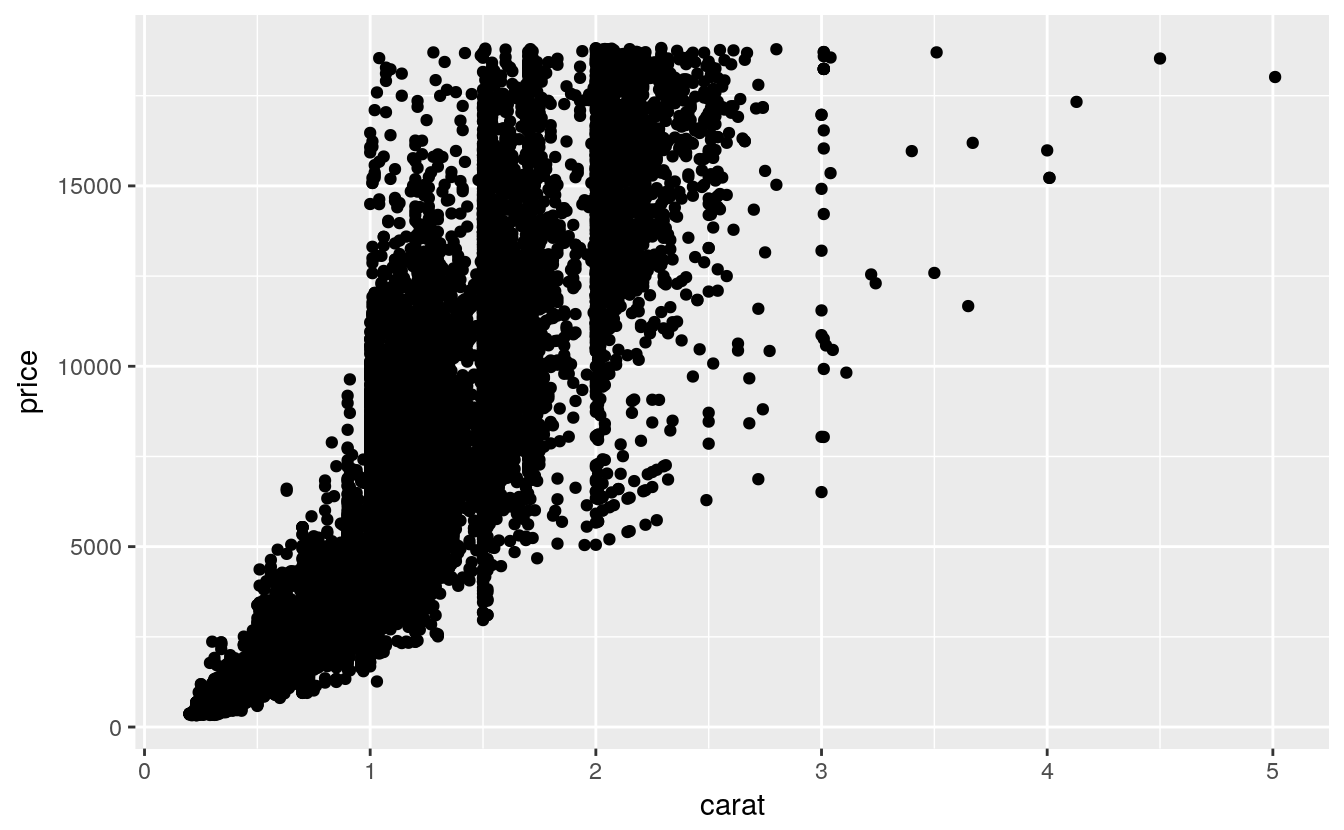
\includegraphics[width=1\linewidth]{bookdown-demo_files/figure-latex/unnamed-chunk-150-1} \end{center}

E se o objetivo for comparar essas relações para diferentes grupos de
lapidação?

\begin{Shaded}
\begin{Highlighting}[]
\KeywordTok{ggplot}\NormalTok{(diamonds, }\KeywordTok{aes}\NormalTok{(}\DataTypeTok{x =}\NormalTok{ carat, }\DataTypeTok{y =}\NormalTok{ price)) }\OperatorTok{+}
\StringTok{  }\KeywordTok{geom_point}\NormalTok{() }\OperatorTok{+}
\StringTok{  }\KeywordTok{facet_wrap}\NormalTok{(}\OperatorTok{~}\StringTok{ }\NormalTok{cut)}
\end{Highlighting}
\end{Shaded}

\begin{center}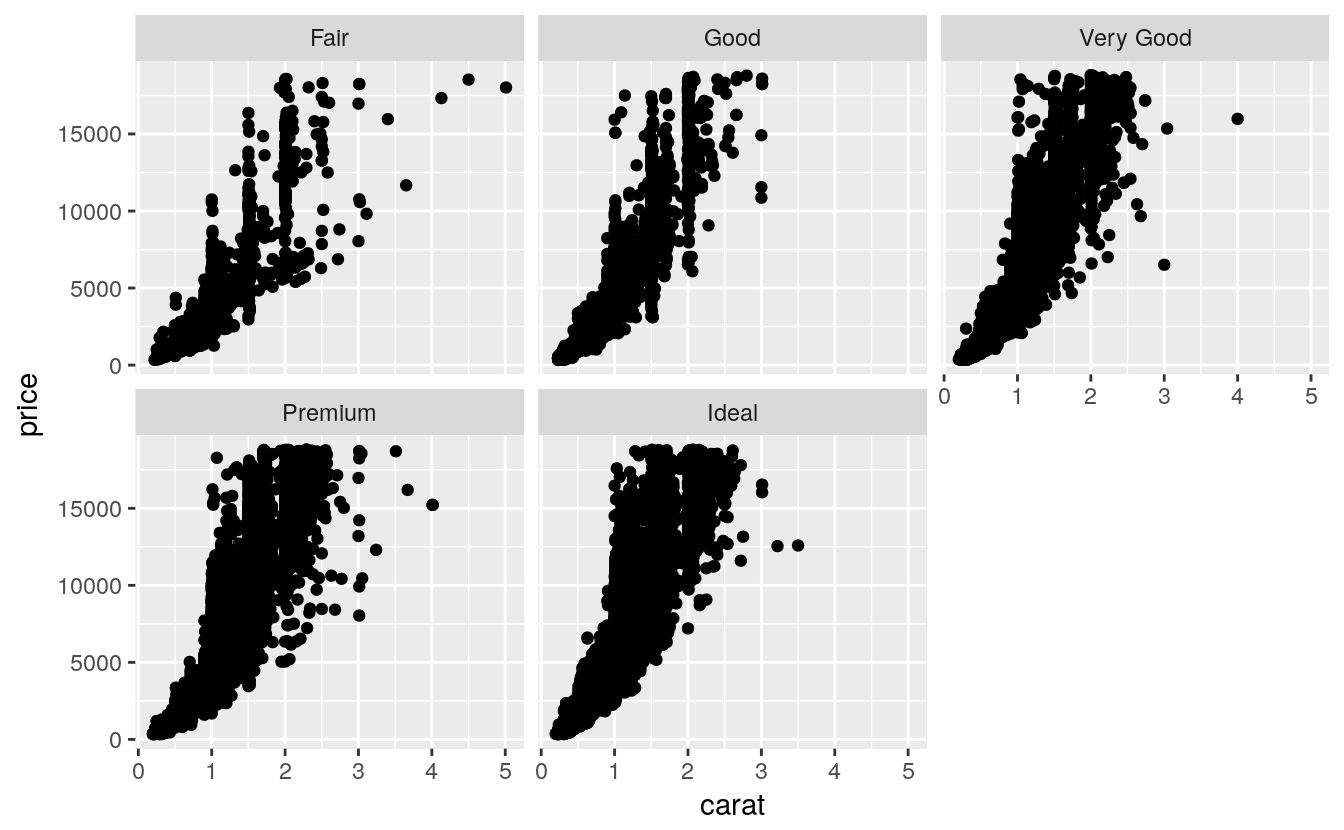
\includegraphics[width=1\linewidth]{bookdown-demo_files/figure-latex/unnamed-chunk-151-1} \end{center}

Usamos a fórmula \texttt{\textasciitilde{}\ cut}. Ou seja, indicamos que
queremos quebrar os gráficos pela variável \texttt{cut}.

O ggplot2 determinou automaticamente o número de colunas e linhas e
fixou as escalas dos eixos. No entanto, podemos definir o número de
linha ou colunas a partir dos argumentos \texttt{nrow} e \texttt{ncol}.
Também é possível definir que cada gráfico tenha sua escala. No exemplo
abaixo, vamos deixar a escala do eixo y livre.

\begin{Shaded}
\begin{Highlighting}[]
\KeywordTok{ggplot}\NormalTok{(diamonds, }\KeywordTok{aes}\NormalTok{(}\DataTypeTok{x =}\NormalTok{ carat, }\DataTypeTok{y =}\NormalTok{ price)) }\OperatorTok{+}
\StringTok{  }\KeywordTok{geom_point}\NormalTok{() }\OperatorTok{+}
\StringTok{  }\KeywordTok{facet_wrap}\NormalTok{(}\OperatorTok{~}\StringTok{ }\NormalTok{cut, }\DataTypeTok{scales =} \StringTok{"free_y"}\NormalTok{)}
\end{Highlighting}
\end{Shaded}

\begin{center}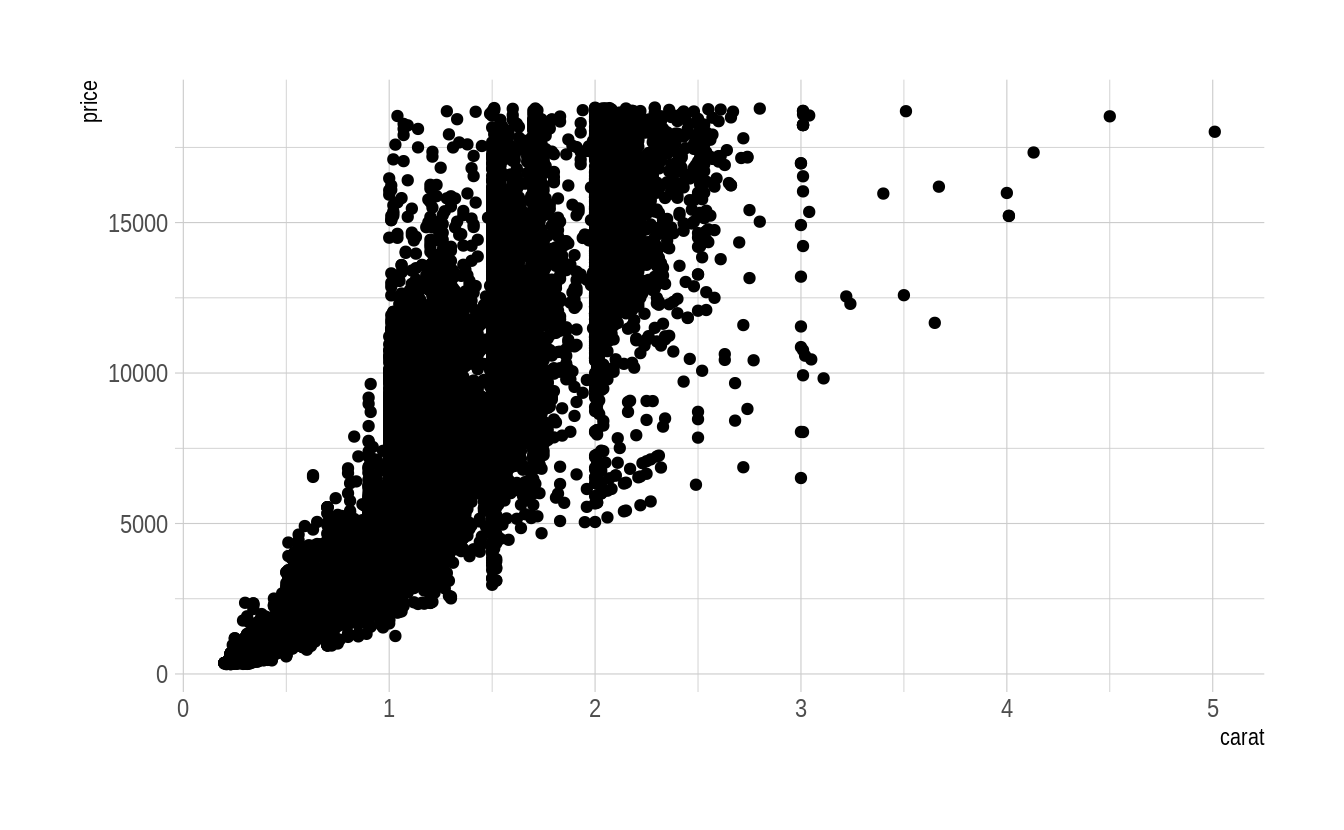
\includegraphics[width=1\linewidth]{bookdown-demo_files/figure-latex/unnamed-chunk-152-1} \end{center}

Já o uso do \texttt{facet\_grid()} é indicado para o cruzamento de
variáveis. No exemplo abaixo, a relação entre as variáveis
\texttt{price} e \texttt{carat} será ``quebrada'' para grupos formados
pelas variáveis \texttt{cut} e \texttt{clarity}:

\begin{Shaded}
\begin{Highlighting}[]
\KeywordTok{ggplot}\NormalTok{(diamonds, }\KeywordTok{aes}\NormalTok{(}\DataTypeTok{x =}\NormalTok{ carat, }\DataTypeTok{y =}\NormalTok{ price)) }\OperatorTok{+}
\StringTok{  }\KeywordTok{geom_point}\NormalTok{() }\OperatorTok{+}
\StringTok{  }\KeywordTok{facet_grid}\NormalTok{(clarity }\OperatorTok{~}\StringTok{ }\NormalTok{cut)}
\end{Highlighting}
\end{Shaded}

\begin{center}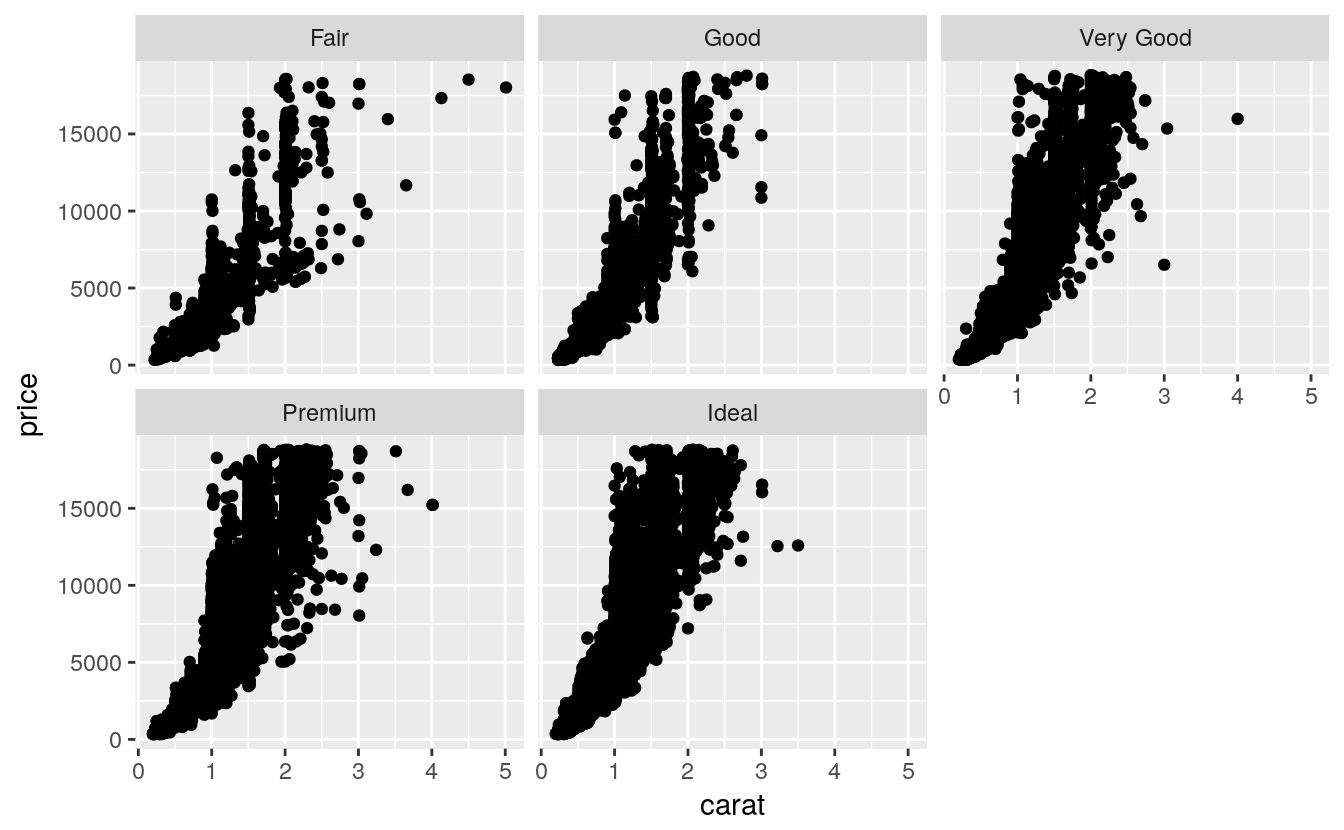
\includegraphics[width=1\linewidth]{bookdown-demo_files/figure-latex/unnamed-chunk-153-1} \end{center}

Note que para cada categoria existe um rótulo. Para alterar esse
relatório, pode-se alterar diretamente o data.frame ou usar a função
\texttt{labeller()}.

\begin{Shaded}
\begin{Highlighting}[]
\NormalTok{nomes_cut <-}\StringTok{ }\KeywordTok{c}\NormalTok{(}
  \DataTypeTok{Fair =} \StringTok{"FAIR"}\NormalTok{,}
  \DataTypeTok{Good =} \StringTok{"GOOD"}\NormalTok{,}
  \StringTok{`}\DataTypeTok{Very Good}\StringTok{`}\NormalTok{ =}\StringTok{ "VERY GOOD"}\NormalTok{,}
  \DataTypeTok{Premium =} \StringTok{"PREMIUM"}\NormalTok{,}
  \DataTypeTok{Ideal =} \StringTok{"IDEAL"}
\NormalTok{)}

\KeywordTok{ggplot}\NormalTok{(diamonds, }\KeywordTok{aes}\NormalTok{(}\DataTypeTok{x =}\NormalTok{ carat, }\DataTypeTok{y =}\NormalTok{ price)) }\OperatorTok{+}
\StringTok{  }\KeywordTok{geom_point}\NormalTok{() }\OperatorTok{+}
\StringTok{  }\KeywordTok{facet_wrap}\NormalTok{(}\OperatorTok{~}\StringTok{ }\NormalTok{cut, }\DataTypeTok{scales =} \StringTok{"free_y"}\NormalTok{,}
             \DataTypeTok{labeller =} \KeywordTok{labeller}\NormalTok{(}\DataTypeTok{cut =}\NormalTok{ nomes_cut))}
\end{Highlighting}
\end{Shaded}

\begin{center}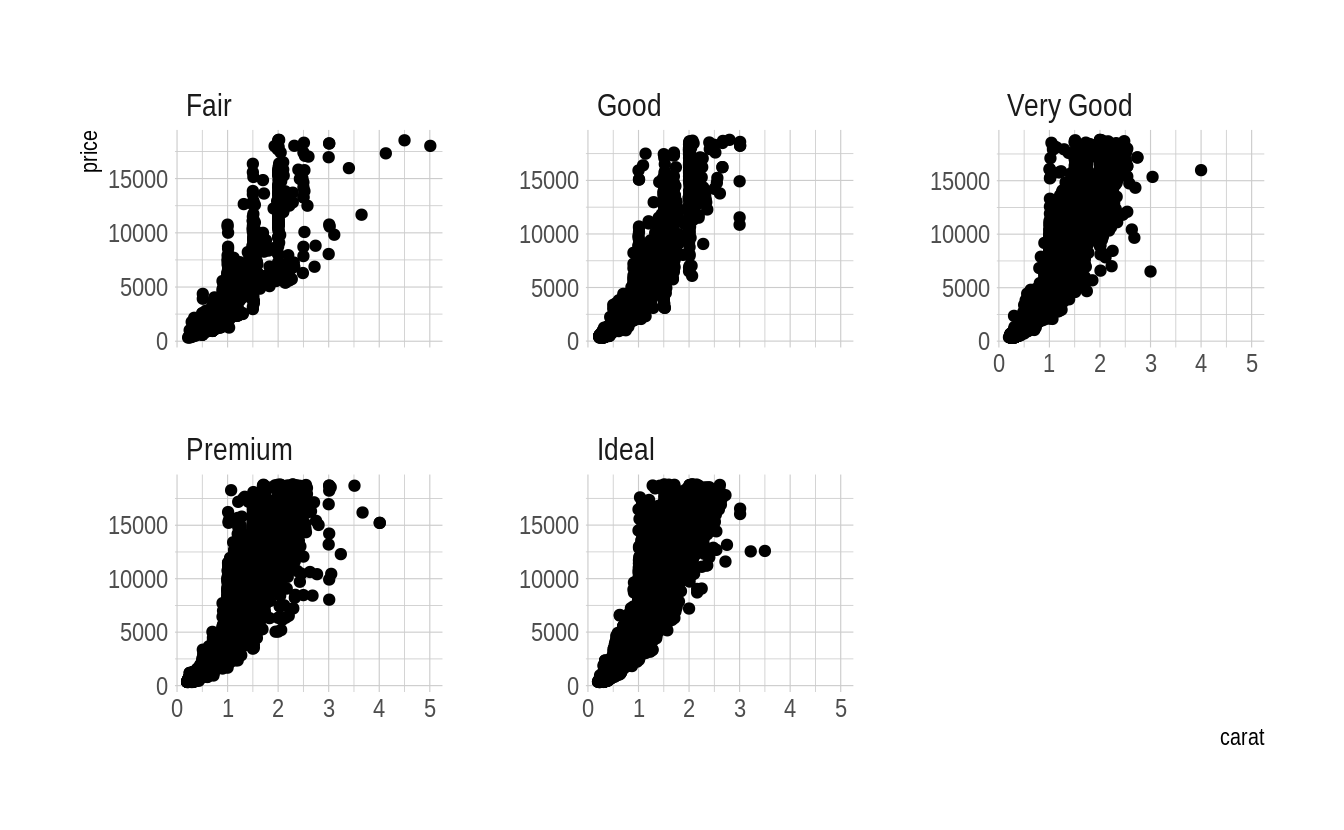
\includegraphics[width=1\linewidth]{bookdown-demo_files/figure-latex/unnamed-chunk-154-1} \end{center}

\section{Temas}\label{temas}

O ggplot2 fornece alguns temas prontos. Todavia, o usuário pode alterar
manualmente cada detalhe de um gráfico ou criar um tema que será
utilizado em outras visualizações. Para editar o tema, será usada a
função \texttt{theme()}. Nessa função, poderão ser alterados os
elementos do tema, como a cor de fundo do painel, o tamanho da fonte do
eixo x, a posição da legenda etc. A lista de elementos estão disponíveis
\href{http://docs.ggplot2.org/current/theme.html}{neste link}.

Para cada elemento do tema, um tipo de objeto é esperado para realizar
alterações. Por exemplo, para alterar o estilo do título do eixo x
(\texttt{axis.title.x}) é preciso passar a função
\texttt{element\_text()}, que possui diversos parâmetros (família da
fonte, tipo da fonte, cor, tamanho, alinhamento etc.). Além do
\texttt{element\_text()}, as principais funções para alterar elementos
do tema são \texttt{element\_line()}, \texttt{element\_rect()} e
\texttt{element\_blank()}. O \texttt{element\_blank()} é usado para que
nada seja desenhado para o elemento que recebe essa função.

Em um primeiro momento, pode parecer complicado ir alterando o tema via
código. Porém, conforme o usuário for praticando, essas alterações vão
ficar mais intuitivas. De toda forma, existe um addin para o RStudio que
ajuda a customizar um gráfico do ggplot2 a partir de uma interface de
\emph{point and click}. Para instalá-lo, faça o seguinte:

\begin{Shaded}
\begin{Highlighting}[]
\KeywordTok{install.packages}\NormalTok{(}\StringTok{'ggThemeAssist'}\NormalTok{)}
\end{Highlighting}
\end{Shaded}

Para exemplificar a alteração do tema manualmente,

\begin{Shaded}
\begin{Highlighting}[]
\KeywordTok{ggplot}\NormalTok{(diamonds, }\KeywordTok{aes}\NormalTok{(}\DataTypeTok{x =}\NormalTok{ carat, }\DataTypeTok{y =}\NormalTok{ price)) }\OperatorTok{+}
\StringTok{  }\KeywordTok{geom_point}\NormalTok{() }\OperatorTok{+}\StringTok{ }
\StringTok{  }\KeywordTok{labs}\NormalTok{(}\DataTypeTok{title =} \StringTok{"Carat vs Price"}\NormalTok{) }\OperatorTok{+}
\StringTok{  }\KeywordTok{theme}\NormalTok{(}\DataTypeTok{text =} \KeywordTok{element_text}\NormalTok{(}\DataTypeTok{face =} \StringTok{"bold"}\NormalTok{), }
        \DataTypeTok{panel.grid.major =} \KeywordTok{element_line}\NormalTok{(}\DataTypeTok{colour =} \StringTok{"gray80"}\NormalTok{), }
        \DataTypeTok{axis.title =} \KeywordTok{element_text}\NormalTok{(}\DataTypeTok{size =} \DecValTok{14}\NormalTok{),}
        \DataTypeTok{panel.background =} \KeywordTok{element_rect}\NormalTok{(}\DataTypeTok{fill =} \StringTok{"gray100"}\NormalTok{))}
\end{Highlighting}
\end{Shaded}

\begin{center}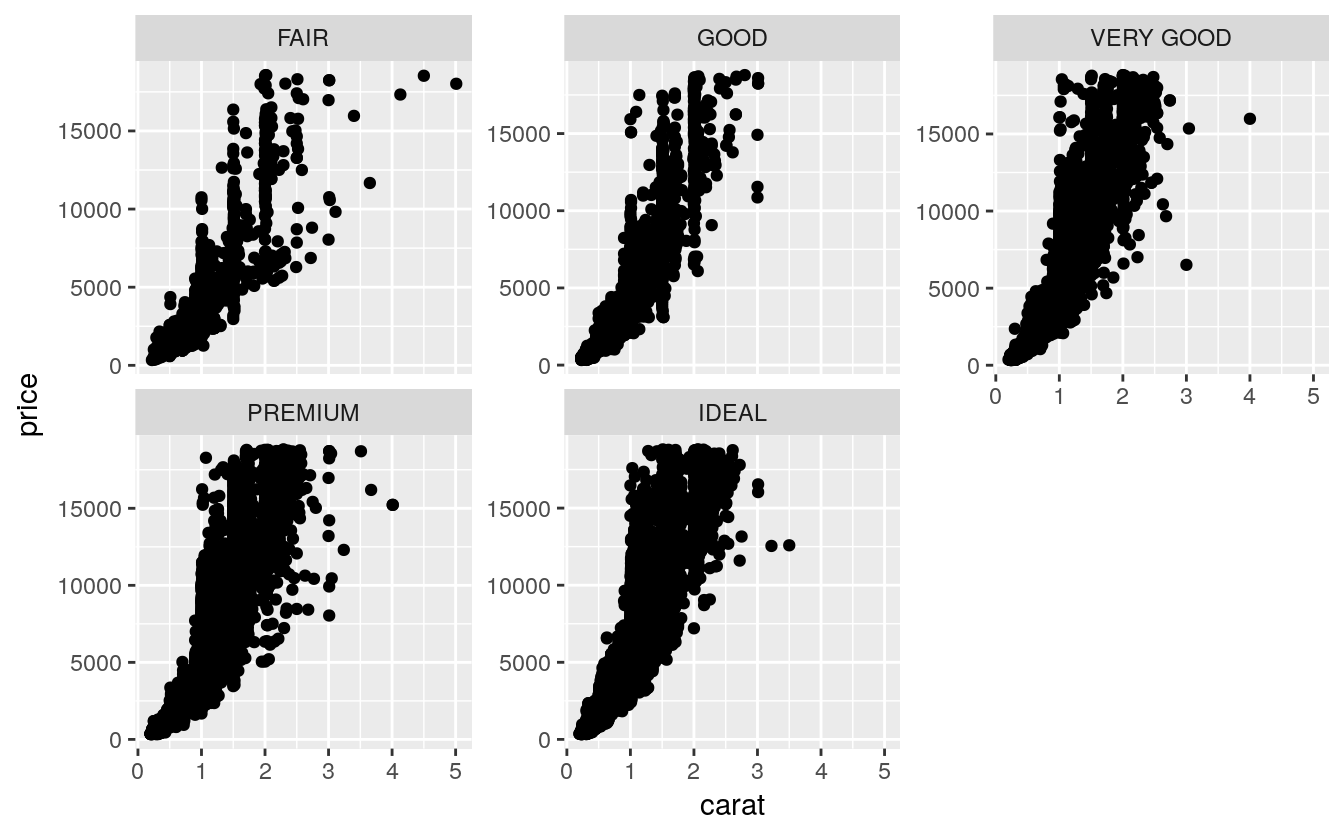
\includegraphics[width=1\linewidth]{bookdown-demo_files/figure-latex/unnamed-chunk-156-1} \end{center}

\subsection{Temas disponíveis no
ggplot2}\label{temas-disponiveis-no-ggplot2}

\begin{Shaded}
\begin{Highlighting}[]
\NormalTok{p <-}\StringTok{ }\KeywordTok{ggplot}\NormalTok{(diamonds, }\KeywordTok{aes}\NormalTok{(}\DataTypeTok{x =}\NormalTok{ carat, }\DataTypeTok{y =}\NormalTok{ price)) }\OperatorTok{+}
\StringTok{  }\KeywordTok{geom_point}\NormalTok{() }
\NormalTok{p }\OperatorTok{+}\StringTok{ }\KeywordTok{theme_gray}\NormalTok{() }\OperatorTok{+}
\StringTok{  }\KeywordTok{labs}\NormalTok{(}\DataTypeTok{title =} \StringTok{"theme_gray()"}\NormalTok{)}

\NormalTok{p }\OperatorTok{+}\StringTok{ }\KeywordTok{theme_bw}\NormalTok{() }\OperatorTok{+}
\StringTok{  }\KeywordTok{labs}\NormalTok{(}\DataTypeTok{title =} \StringTok{"theme_bw()"}\NormalTok{)}

\NormalTok{p }\OperatorTok{+}\StringTok{ }\KeywordTok{theme_linedraw}\NormalTok{() }\OperatorTok{+}
\StringTok{  }\KeywordTok{labs}\NormalTok{(}\DataTypeTok{title =} \StringTok{"theme_linedraw()"}\NormalTok{)}

\NormalTok{p }\OperatorTok{+}\StringTok{ }\KeywordTok{theme_light}\NormalTok{() }\OperatorTok{+}
\StringTok{  }\KeywordTok{labs}\NormalTok{(}\DataTypeTok{title =} \StringTok{"theme_light()"}\NormalTok{)}

\NormalTok{p }\OperatorTok{+}\StringTok{ }\KeywordTok{theme_minimal}\NormalTok{() }\OperatorTok{+}
\StringTok{  }\KeywordTok{labs}\NormalTok{(}\DataTypeTok{title =} \StringTok{"theme_minimal()"}\NormalTok{)}

\NormalTok{p }\OperatorTok{+}\StringTok{ }\KeywordTok{theme_classic}\NormalTok{() }\OperatorTok{+}
\StringTok{  }\KeywordTok{labs}\NormalTok{(}\DataTypeTok{title =} \StringTok{"theme_classic()"}\NormalTok{)}

\NormalTok{p }\OperatorTok{+}\StringTok{ }\KeywordTok{theme_dark}\NormalTok{() }\OperatorTok{+}
\StringTok{  }\KeywordTok{labs}\NormalTok{(}\DataTypeTok{title =} \StringTok{"theme_dark()"}\NormalTok{)}

\NormalTok{p }\OperatorTok{+}\StringTok{ }\KeywordTok{theme_void}\NormalTok{() }\OperatorTok{+}
\StringTok{  }\KeywordTok{labs}\NormalTok{(}\DataTypeTok{title =} \StringTok{"theme_void()"}\NormalTok{)}
\end{Highlighting}
\end{Shaded}

\begin{center}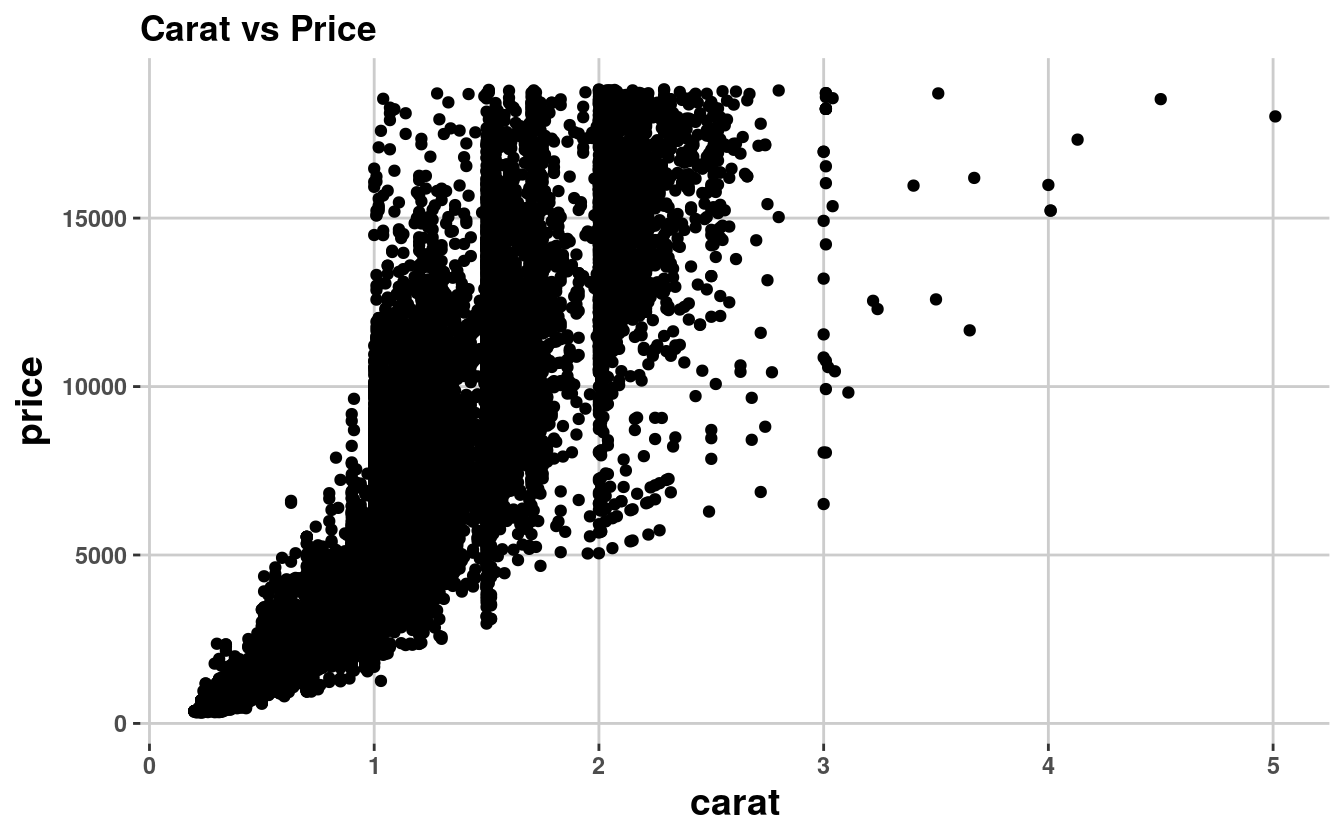
\includegraphics[width=1\linewidth]{bookdown-demo_files/figure-latex/unnamed-chunk-158-1} \end{center}

\subsection{Temas no pacote ggthemes}\label{temas-no-pacote-ggthemes}

O pacote \href{https://github.com/jrnold/ggthemes}{\texttt{ggthemes}}
disponibiliza um conjuntos de temas e escalas de cores. Vamos apresentar
alguns temas disponíveis.

\begin{center}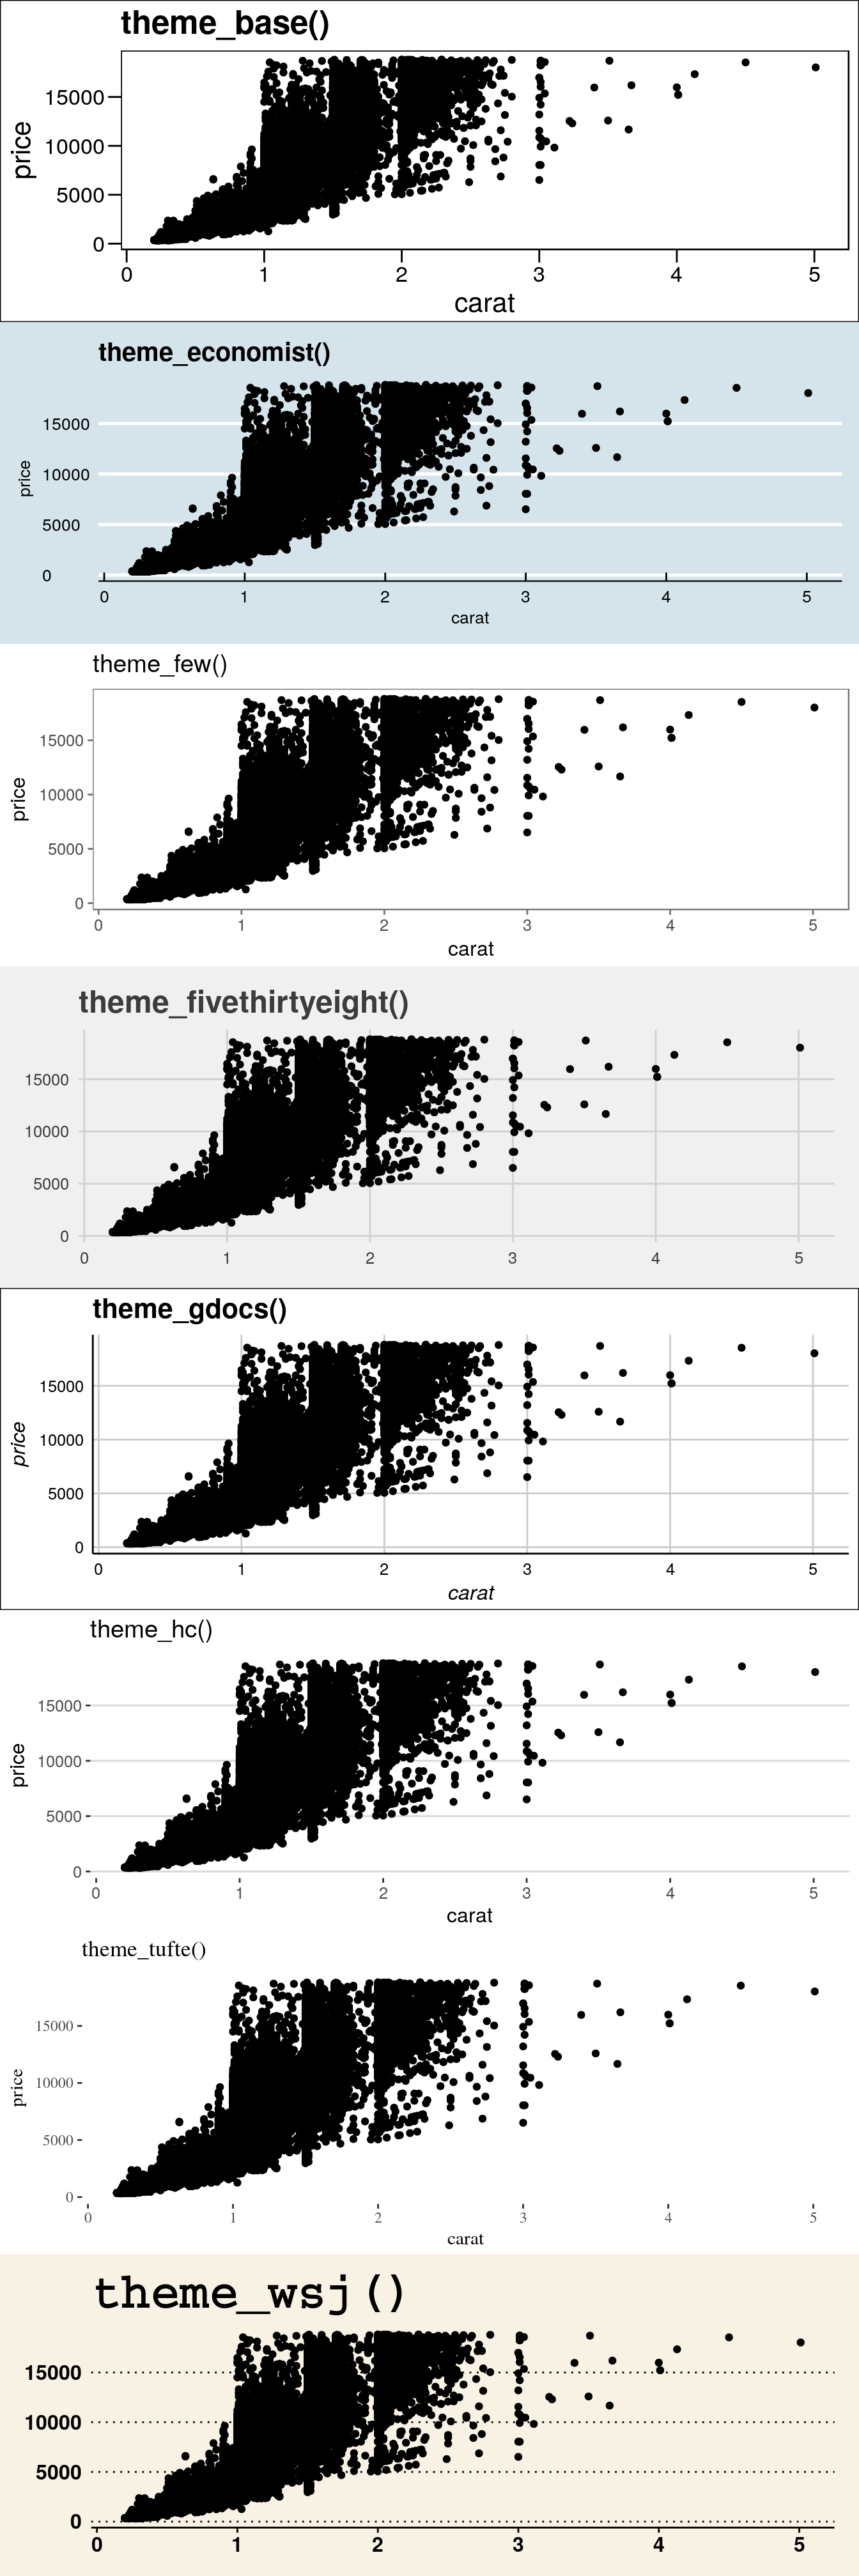
\includegraphics[width=1\linewidth]{bookdown-demo_files/figure-latex/unnamed-chunk-159-1} \end{center}

\begin{center}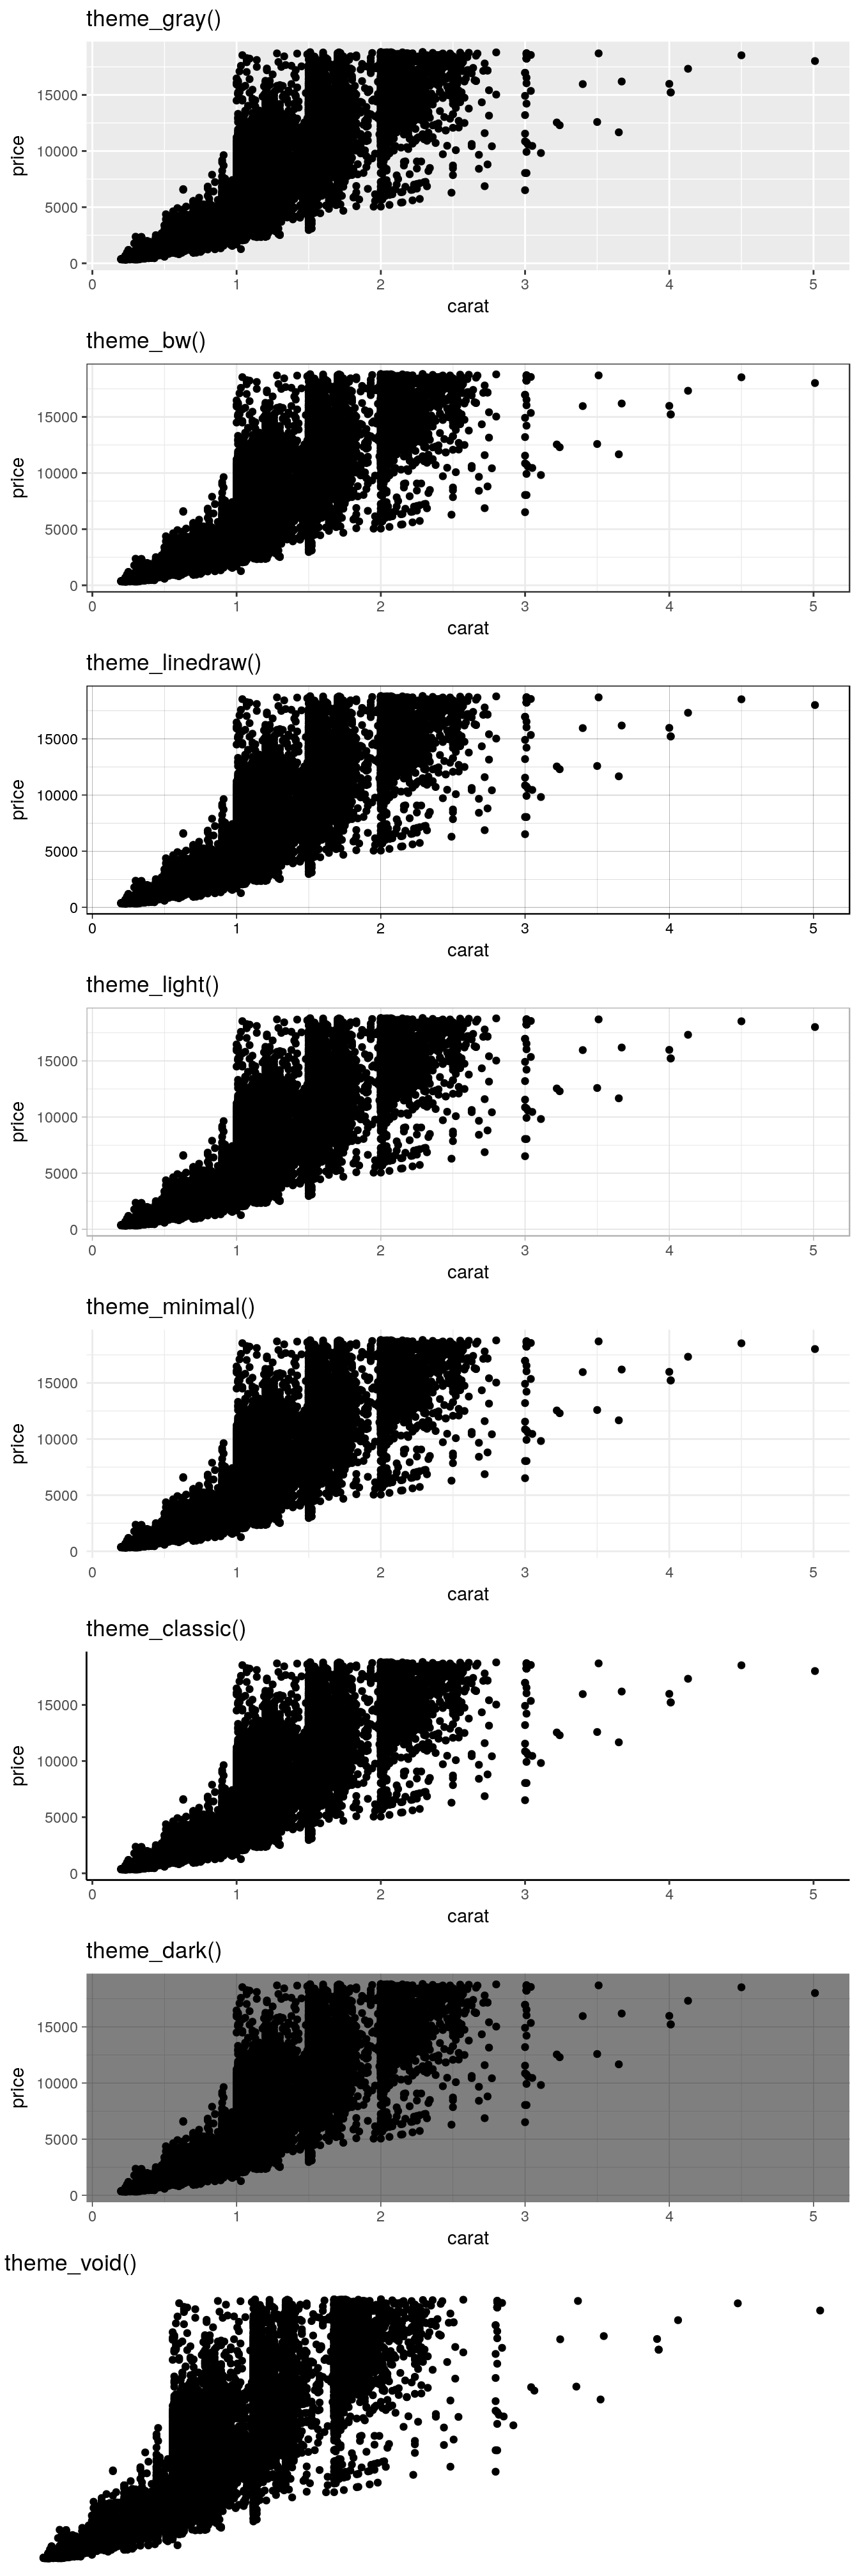
\includegraphics[width=1\linewidth]{bookdown-demo_files/figure-latex/unnamed-chunk-160-1} \end{center}

\subsection{hrbrthemes}\label{hrbrthemes}

Alguns pacotes fornecem seus próprios temas. É o caso do
\texttt{hrbrthemes}. Esse pacote fornece um tema bastante interessante e
será usado no resto desse capítulo. Como qualquer outro tema, se for
necessário, você pode editar esse tema com a função \texttt{theme()}

\begin{Shaded}
\begin{Highlighting}[]
\KeywordTok{install.packages}\NormalTok{(}\StringTok{"hrbrthemes"}\NormalTok{)}
\end{Highlighting}
\end{Shaded}

\begin{Shaded}
\begin{Highlighting}[]
\KeywordTok{library}\NormalTok{(hrbrthemes)}
\KeywordTok{ggplot}\NormalTok{(diamonds, }\KeywordTok{aes}\NormalTok{(}\DataTypeTok{x =}\NormalTok{ carat, }\DataTypeTok{y =}\NormalTok{ price)) }\OperatorTok{+}
\StringTok{  }\KeywordTok{geom_point}\NormalTok{() }\OperatorTok{+}
\StringTok{  }\KeywordTok{labs}\NormalTok{(}\DataTypeTok{title =} \StringTok{"theme_ipsum()"}\NormalTok{) }\OperatorTok{+}
\StringTok{  }\KeywordTok{theme_ipsum}\NormalTok{(}\DataTypeTok{plot_title_size =} \DecValTok{12}\NormalTok{,}
              \DataTypeTok{axis_title_size =} \DecValTok{10}\NormalTok{)}
\end{Highlighting}
\end{Shaded}

\begin{center}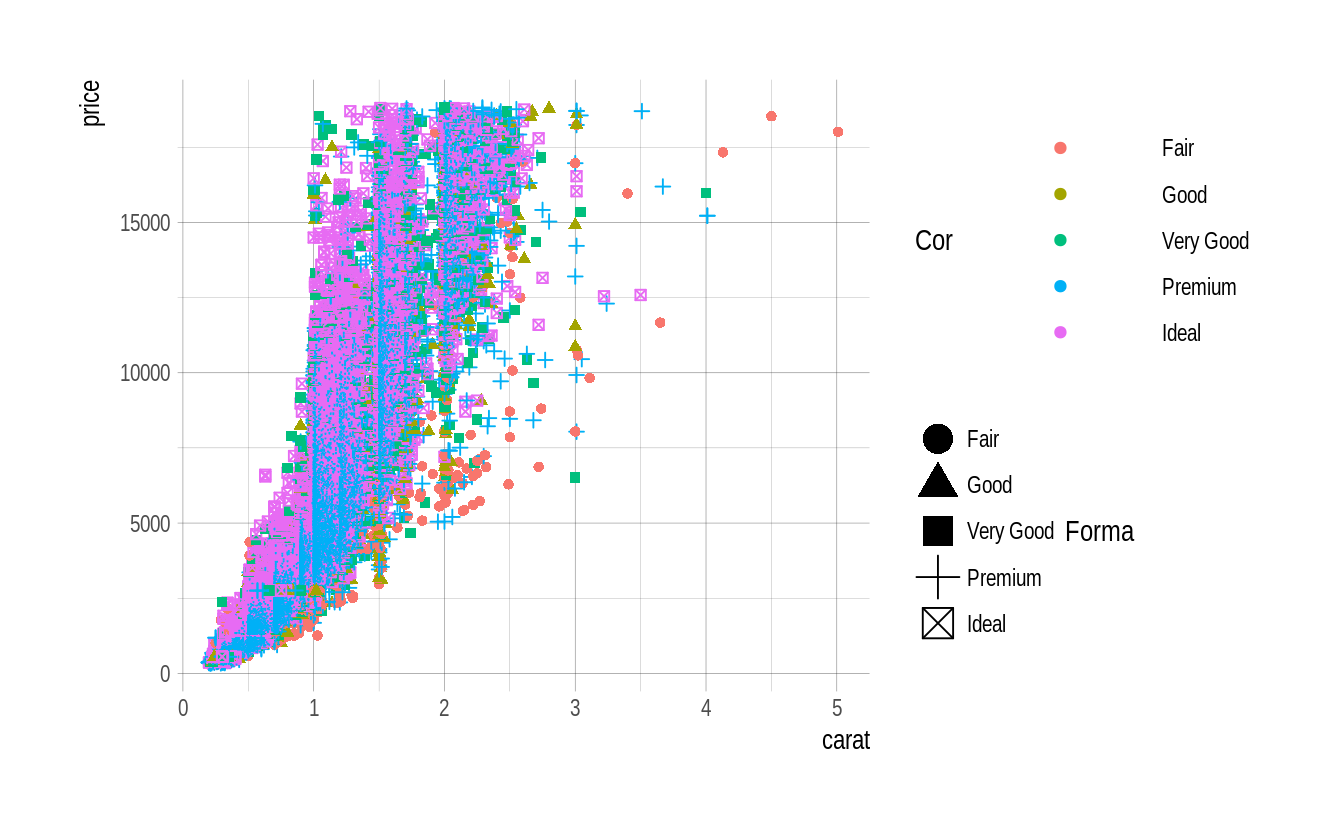
\includegraphics[width=1\linewidth]{bookdown-demo_files/figure-latex/unnamed-chunk-162-1} \end{center}

\subsection{Setando o tema
globalmente}\label{setando-o-tema-globalmente}

Com o comando abaixo todos os gráficos do seu script terão o mesmo tema:

\begin{Shaded}
\begin{Highlighting}[]
\KeywordTok{theme_set}\NormalTok{(}\KeywordTok{theme_ipsum}\NormalTok{(}\DataTypeTok{plot_title_size =} \DecValTok{12}\NormalTok{,}
              \DataTypeTok{axis_title_size =} \DecValTok{10}\NormalTok{) }\OperatorTok{+}
\StringTok{          }\KeywordTok{theme}\NormalTok{(}\DataTypeTok{text =} \KeywordTok{element_text}\NormalTok{(}\DataTypeTok{angle =} \DecValTok{0}\NormalTok{)))}
\end{Highlighting}
\end{Shaded}

\section{Legendas}\label{legendas}

Parte das alterações das legendas pode ser feita via \texttt{theme()}.
Essas alterações são gerais para todas as legendas. Se o interesse for
em mudanças pontuais na legenda de algum elemento estético, serão
utilizadas as funções \texttt{guides()}, \texttt{guide\_legend()} e
\texttt{guide\_colorbar()}.

\begin{Shaded}
\begin{Highlighting}[]
\KeywordTok{guide_legend}\NormalTok{(}\DataTypeTok{title =} \KeywordTok{waiver}\NormalTok{(), }\DataTypeTok{title.position =} \OtherTok{NULL}\NormalTok{, }\DataTypeTok{title.theme =} \OtherTok{NULL}\NormalTok{,}
             \DataTypeTok{title.hjust =} \OtherTok{NULL}\NormalTok{, }\DataTypeTok{title.vjust =} \OtherTok{NULL}\NormalTok{, }\DataTypeTok{label =} \OtherTok{TRUE}\NormalTok{,}
             \DataTypeTok{label.position =} \OtherTok{NULL}\NormalTok{, }\DataTypeTok{label.theme =} \OtherTok{NULL}\NormalTok{, }\DataTypeTok{label.hjust =} \OtherTok{NULL}\NormalTok{,}
             \DataTypeTok{label.vjust =} \OtherTok{NULL}\NormalTok{, }\DataTypeTok{keywidth =} \OtherTok{NULL}\NormalTok{, }\DataTypeTok{keyheight =} \OtherTok{NULL}\NormalTok{,}
             \DataTypeTok{direction =} \OtherTok{NULL}\NormalTok{, }\DataTypeTok{default.unit =} \StringTok{"line"}\NormalTok{, }\DataTypeTok{override.aes =} \KeywordTok{list}\NormalTok{(),}
             \DataTypeTok{nrow =} \OtherTok{NULL}\NormalTok{, }\DataTypeTok{ncol =} \OtherTok{NULL}\NormalTok{, }\DataTypeTok{byrow =} \OtherTok{FALSE}\NormalTok{, }\DataTypeTok{reverse =} \OtherTok{FALSE}\NormalTok{, }\DataTypeTok{order =} \DecValTok{0}\NormalTok{, ...)}

\KeywordTok{guide_colourbar}\NormalTok{(}\DataTypeTok{title =} \KeywordTok{waiver}\NormalTok{(), }\DataTypeTok{title.position =} \OtherTok{NULL}\NormalTok{, }\DataTypeTok{title.theme =} \OtherTok{NULL}\NormalTok{,}
                \DataTypeTok{title.hjust =} \OtherTok{NULL}\NormalTok{, }\DataTypeTok{title.vjust =} \OtherTok{NULL}\NormalTok{, }\DataTypeTok{label =} \OtherTok{TRUE}\NormalTok{,}
                \DataTypeTok{label.position =} \OtherTok{NULL}\NormalTok{, }\DataTypeTok{label.theme =} \OtherTok{NULL}\NormalTok{, }\DataTypeTok{label.hjust =} \OtherTok{NULL}\NormalTok{,}
                \DataTypeTok{label.vjust =} \OtherTok{NULL}\NormalTok{, }\DataTypeTok{barwidth =} \OtherTok{NULL}\NormalTok{, }\DataTypeTok{barheight =} \OtherTok{NULL}\NormalTok{, }\DataTypeTok{nbin =} \DecValTok{20}\NormalTok{,}
                \DataTypeTok{raster =} \OtherTok{TRUE}\NormalTok{, }\DataTypeTok{ticks =} \OtherTok{TRUE}\NormalTok{, }\DataTypeTok{draw.ulim =} \OtherTok{TRUE}\NormalTok{, }\DataTypeTok{draw.llim =} \OtherTok{TRUE}\NormalTok{,}
                \DataTypeTok{direction =} \OtherTok{NULL}\NormalTok{, }\DataTypeTok{default.unit =} \StringTok{"line"}\NormalTok{, }\DataTypeTok{reverse =} \OtherTok{FALSE}\NormalTok{, }\DataTypeTok{order =} \DecValTok{0}\NormalTok{, ...)}
\end{Highlighting}
\end{Shaded}

O código abaixo exemplifica o uso do \texttt{guide\_legend()}.

\begin{Shaded}
\begin{Highlighting}[]
\KeywordTok{ggplot}\NormalTok{(diamonds, }\KeywordTok{aes}\NormalTok{(}\DataTypeTok{x =}\NormalTok{ carat, }\DataTypeTok{y =}\NormalTok{ price, }\DataTypeTok{color =}\NormalTok{ cut, }\DataTypeTok{shape =}\NormalTok{ cut)) }\OperatorTok{+}
\StringTok{  }\KeywordTok{geom_point}\NormalTok{() }\OperatorTok{+}
\StringTok{  }\KeywordTok{guides}\NormalTok{(}\DataTypeTok{color =} \KeywordTok{guide_legend}\NormalTok{(}\DataTypeTok{title =} \StringTok{"Cor"}\NormalTok{, }\DataTypeTok{title.position =} \StringTok{"left"}\NormalTok{, }\DataTypeTok{keywidth =} \DecValTok{5}\NormalTok{),}
         \DataTypeTok{shape =} \KeywordTok{guide_legend}\NormalTok{(}\DataTypeTok{title =} \StringTok{"Forma"}\NormalTok{, }\DataTypeTok{title.position =} \StringTok{"right"}\NormalTok{, }\DataTypeTok{override.aes =} \KeywordTok{aes}\NormalTok{(}\DataTypeTok{size =} \DecValTok{5}\NormalTok{)))}
\end{Highlighting}
\end{Shaded}

\begin{center}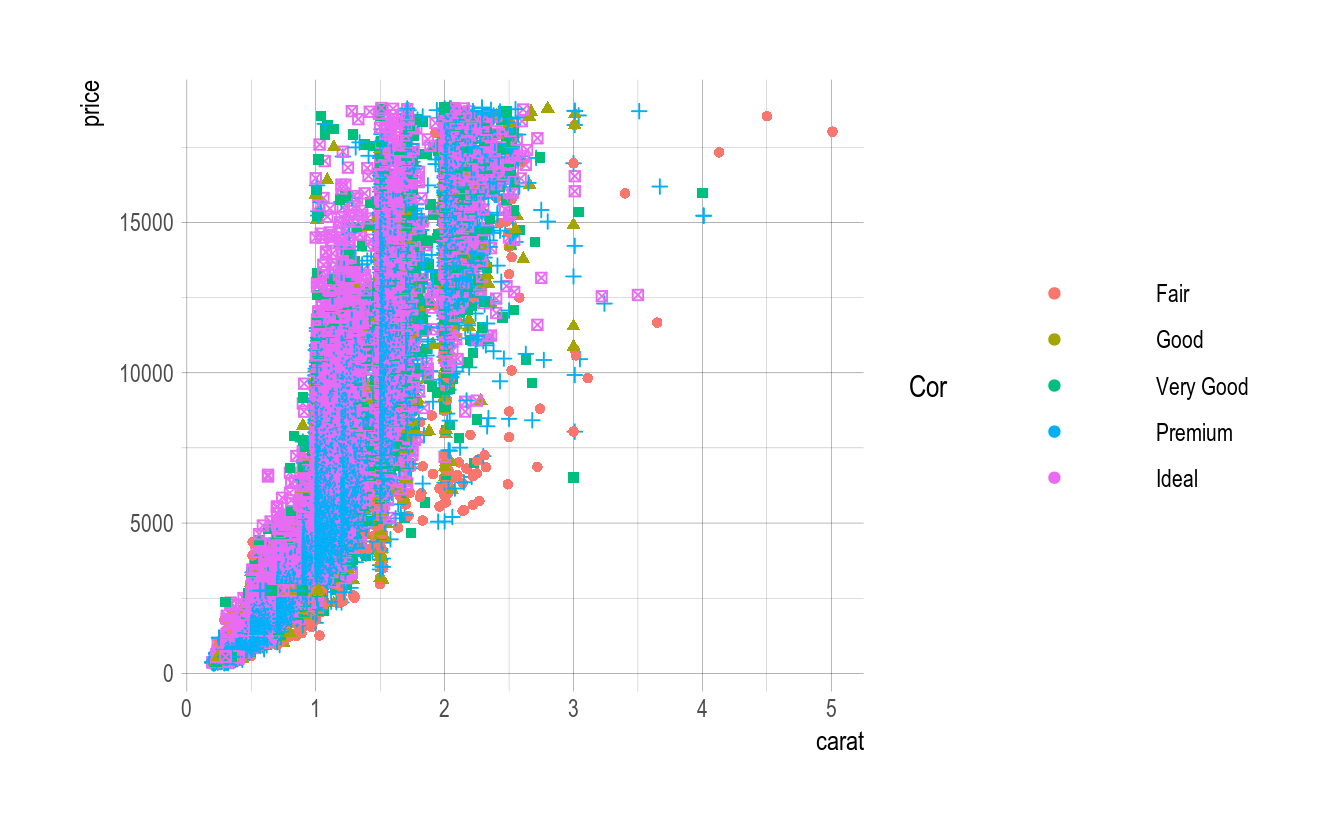
\includegraphics[width=1\linewidth]{bookdown-demo_files/figure-latex/unnamed-chunk-165-1} \end{center}

Pode-se fazer uso do ``none'' para omitir a legenda de um elemento
estético:

\begin{Shaded}
\begin{Highlighting}[]
\KeywordTok{ggplot}\NormalTok{(diamonds, }\KeywordTok{aes}\NormalTok{(}\DataTypeTok{x =}\NormalTok{ carat, }\DataTypeTok{y =}\NormalTok{ price, }\DataTypeTok{color =}\NormalTok{ cut, }\DataTypeTok{shape =}\NormalTok{ cut)) }\OperatorTok{+}
\StringTok{  }\KeywordTok{geom_point}\NormalTok{() }\OperatorTok{+}
\StringTok{  }\KeywordTok{guides}\NormalTok{(}\DataTypeTok{color =} \KeywordTok{guide_legend}\NormalTok{(}\DataTypeTok{title =} \StringTok{"Cor"}\NormalTok{, }\DataTypeTok{title.position =} \StringTok{"left"}\NormalTok{, }\DataTypeTok{keywidth =} \DecValTok{5}\NormalTok{),}
         \DataTypeTok{shape =} \StringTok{"none"}\NormalTok{)}
\end{Highlighting}
\end{Shaded}

\begin{center}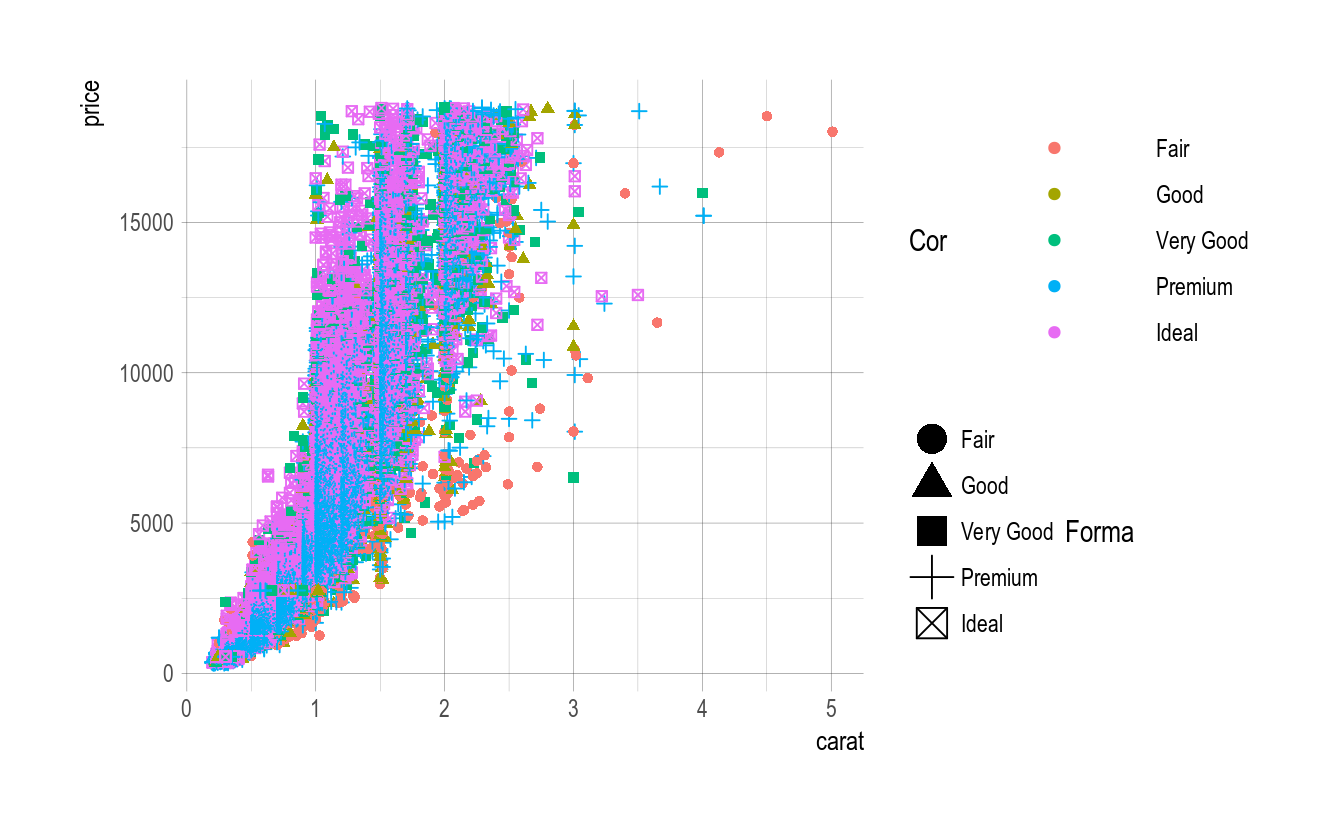
\includegraphics[width=1\linewidth]{bookdown-demo_files/figure-latex/unnamed-chunk-166-1} \end{center}

\section{Escolhendo o tipo de
gráfico}\label{escolhendo-o-tipo-de-grafico}

Antes de decidir qual gráfico você irá utilizar, é preciso saber o que
se deseja representar. O objetivo guiará qual o tipo de gráfico é mais
adequado. A imagem abaixo apresenta uma lista bastante completa de
possibilidades de gráficos, dos mais simples aos mais complexos.

\begin{figure}
\centering
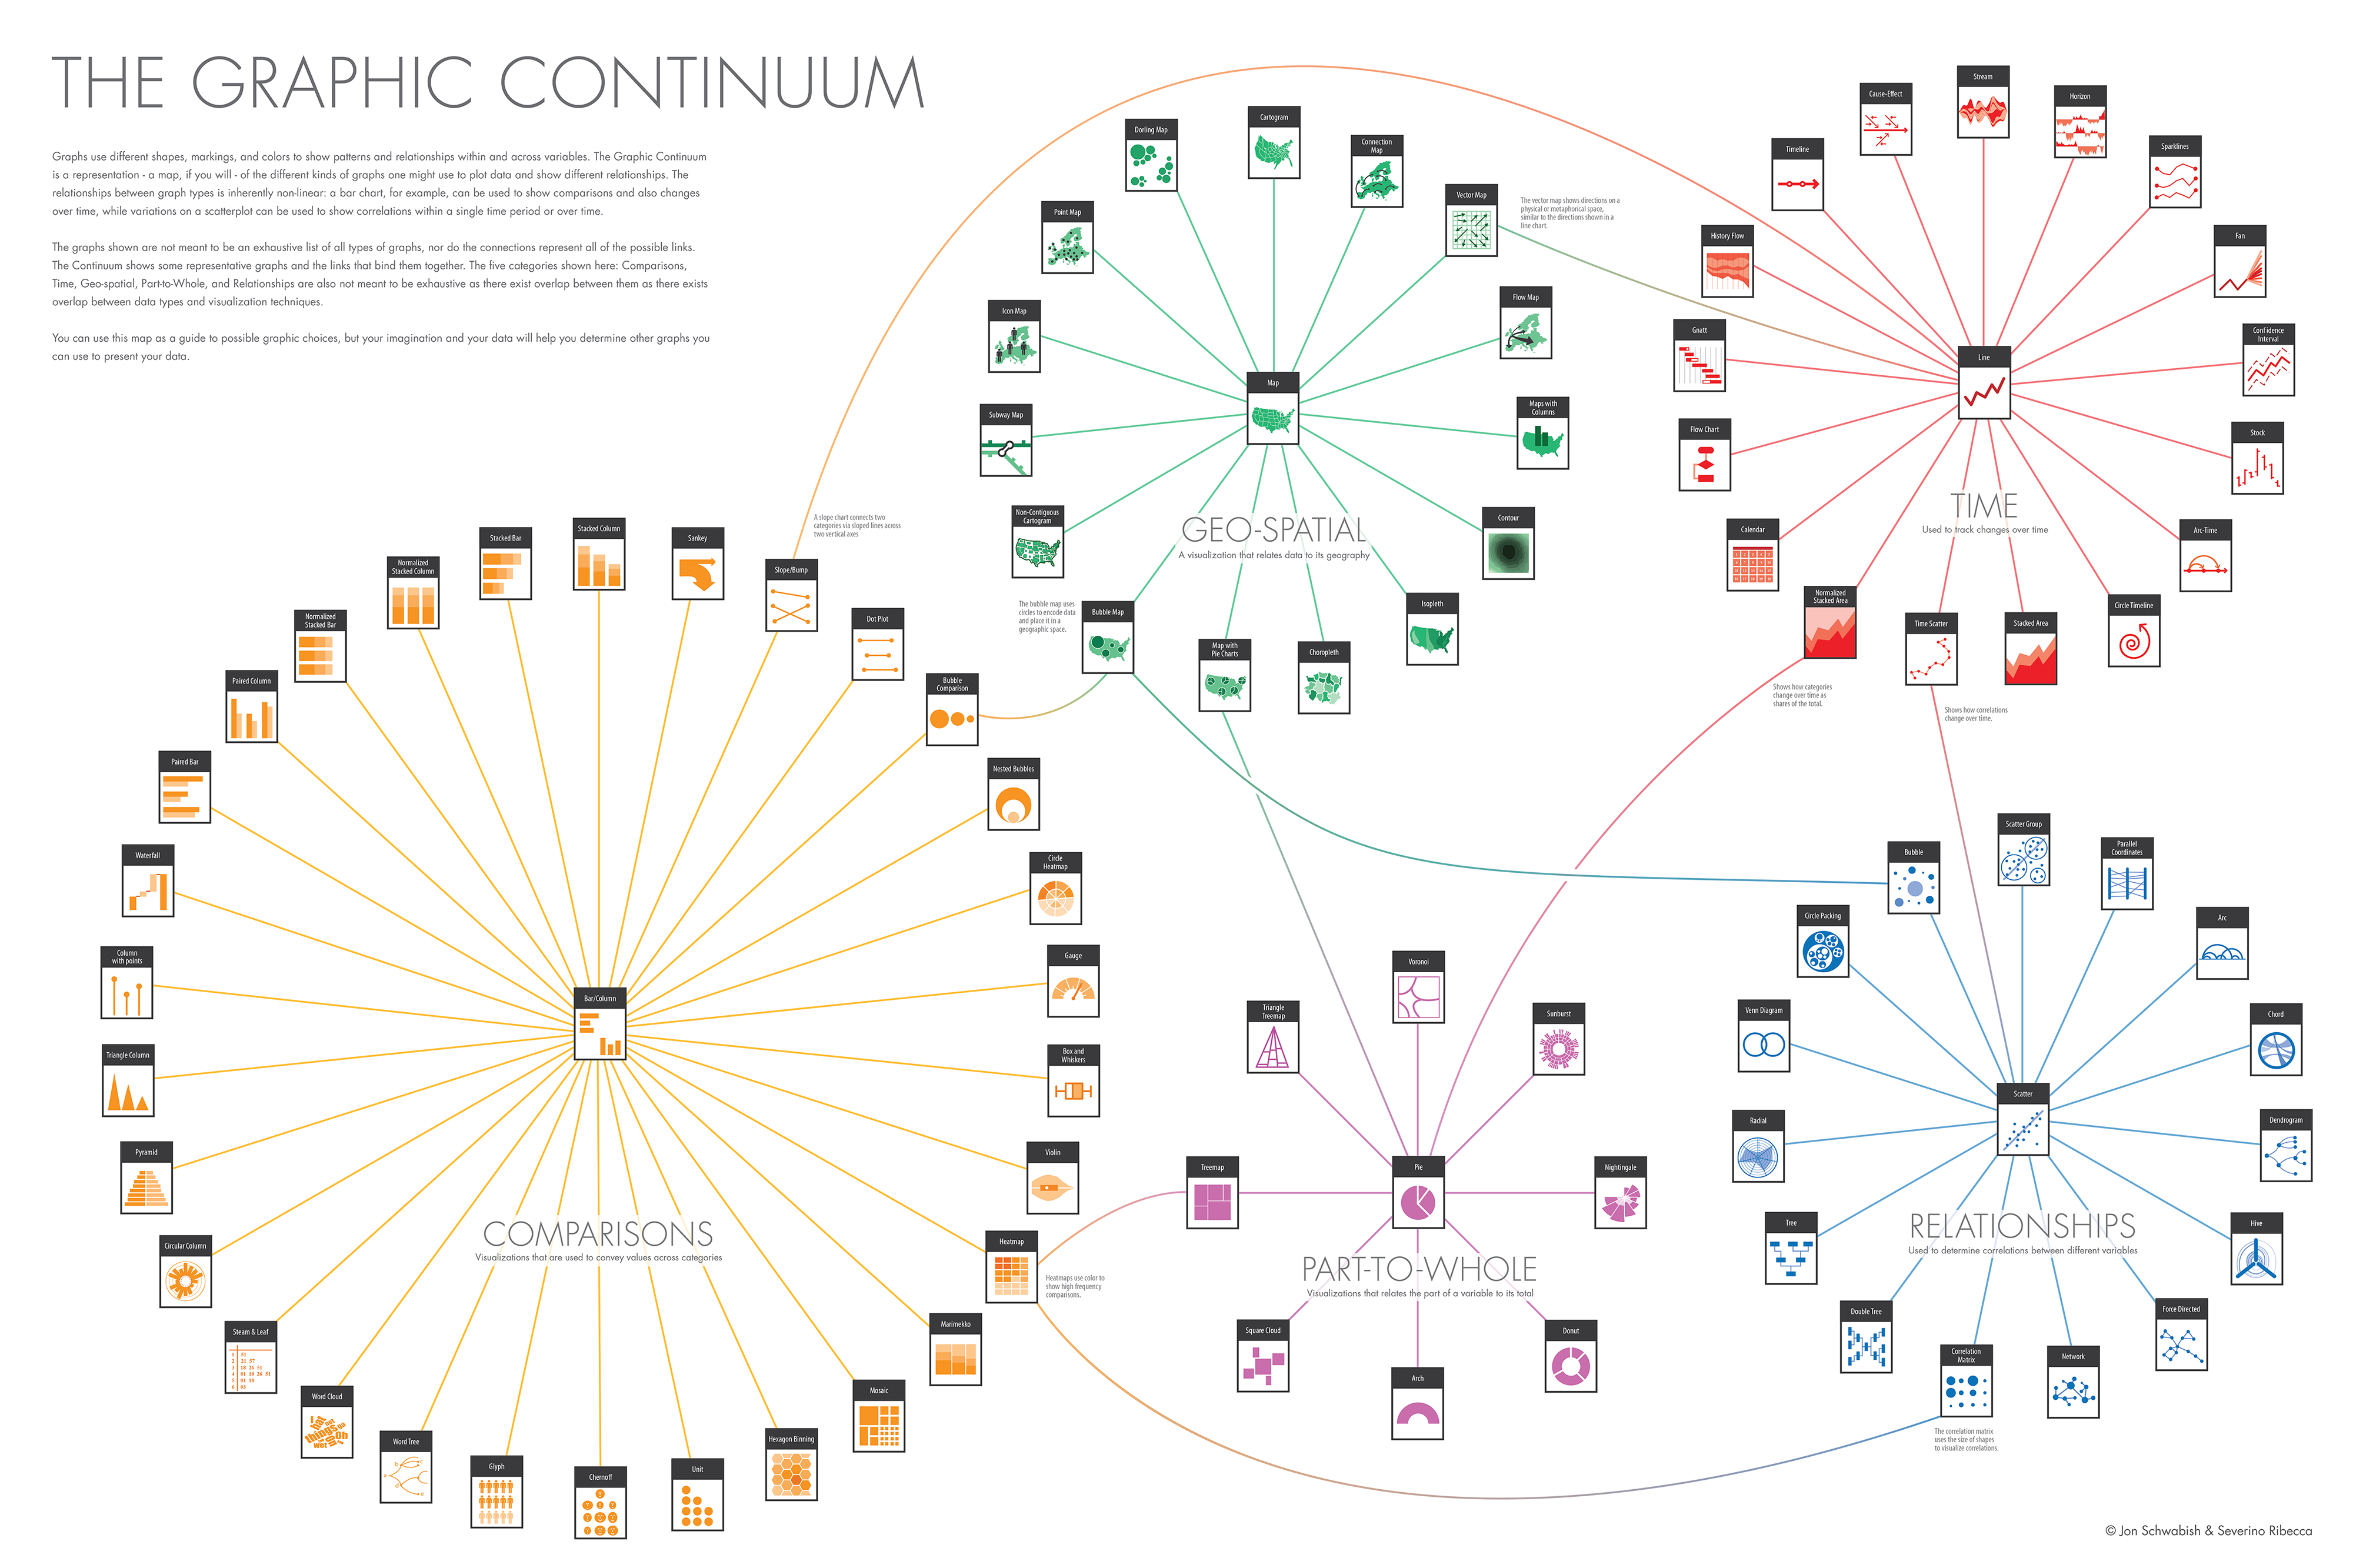
\includegraphics{images/tipo_graficos.png}
\caption{}
\end{figure}

Entre
\href{https://camo.githubusercontent.com/ea2e9eda9b01fafc1213f5c400aa357584f40df8/687474703a2f2f626c6f672e76697375616c2e6c792f77702d636f6e74656e742f75706c6f6164732f323031342f30392f696d6167652d362e706e67}{neste
link} para visualizar a imagem com zoom.

Os gráficos mais tradicionais podem ser facilmente criados a partir da
lógica de camadas do ggplot2 e dos objetos geométricos disponíveis no
pacote. Para gráficos mais complexos, alguns pacotes estão disponíveis.
Por exemplo, para criação de treemaps, existe o pacote
\texttt{treemapify}.

\begin{Shaded}
\begin{Highlighting}[]
\KeywordTok{library}\NormalTok{(treemapify)}

\KeywordTok{ggplot}\NormalTok{(G20, }\KeywordTok{aes}\NormalTok{(}\DataTypeTok{area =}\NormalTok{ gdp_mil_usd, }\DataTypeTok{fill =}\NormalTok{ hdi, }\DataTypeTok{label =}\NormalTok{ country)) }\OperatorTok{+}
\StringTok{  }\KeywordTok{geom_treemap}\NormalTok{() }\OperatorTok{+}
\StringTok{  }\KeywordTok{geom_treemap_text}\NormalTok{(}\DataTypeTok{fontface =} \StringTok{"italic"}\NormalTok{, }\DataTypeTok{colour =} \StringTok{"white"}\NormalTok{, }\DataTypeTok{place =} \StringTok{"centre"}\NormalTok{,}
                    \DataTypeTok{grow =} \OtherTok{TRUE}\NormalTok{) }\OperatorTok{+}
\StringTok{  }\KeywordTok{theme}\NormalTok{(}\DataTypeTok{legend.position =} \StringTok{'bottom'}\NormalTok{)}
\end{Highlighting}
\end{Shaded}

\begin{figure}
\centering
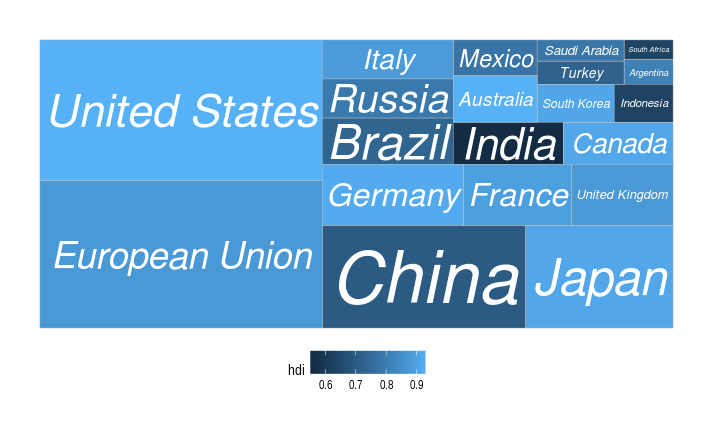
\includegraphics{images/treemapify.png}
\caption{}
\end{figure}

\section{\texorpdfstring{Gráfico de Dispersão
(\texttt{geom\_point()})}{Gráfico de Dispersão (geom\_point())}}\label{grafico-de-dispersao-geom_point}

\begin{Shaded}
\begin{Highlighting}[]
\KeywordTok{geom_point}\NormalTok{(}\DataTypeTok{mapping =} \OtherTok{NULL}\NormalTok{, }\DataTypeTok{data =} \OtherTok{NULL}\NormalTok{, }\DataTypeTok{stat =} \StringTok{"identity"}\NormalTok{, }\DataTypeTok{position =} \StringTok{"identity"}\NormalTok{,}
\NormalTok{           ..., }\DataTypeTok{na.rm =} \OtherTok{FALSE}\NormalTok{, }\DataTypeTok{show.legend =} \OtherTok{NA}\NormalTok{, }\DataTypeTok{inherit.aes =} \OtherTok{TRUE}\NormalTok{)}
\end{Highlighting}
\end{Shaded}

O gráfico de dispersão é bastante usado para verificar relações entre
duas variáveis quantitativas. Para exemplificar, vamos utilizar a base
disponível no pacote \texttt{gapminder}. Nessa base, existem uma
variável de expectativa de vida e outra de renda per capita.

Como queremos um gráfico de pontos, o objeto geométrico natural é o
\texttt{geom\_point()}. Esse objeto geométrico tem os seguintes
elementos estéticos:

Os parâmetros estéticos (aes) são:

\begin{itemize}
\tightlist
\item
  \textbf{\texttt{x}}
\item
  \textbf{\texttt{y}}
\item
  \texttt{alpha}
\item
  \texttt{colour}
\item
  \texttt{fill}
\item
  \texttt{shape}
\item
  \texttt{size}
\item
  \texttt{stroke}
\end{itemize}

Vamos verificar qual é a relação entre essas duas variáveis:

\begin{Shaded}
\begin{Highlighting}[]
\KeywordTok{library}\NormalTok{(hrbrthemes)}
\KeywordTok{library}\NormalTok{(gapminder)}
\NormalTok{gapminder }\OperatorTok\StringTok{ }
\StringTok{  }\KeywordTok{filter}\NormalTok{(year }\OperatorTok{==}\StringTok{ }\KeywordTok{max}\NormalTok{(year)) }\OperatorTok\StringTok{ }
\StringTok{  }\KeywordTok{ggplot}\NormalTok{(}\KeywordTok{aes}\NormalTok{(}\DataTypeTok{x =}\NormalTok{ gdpPercap, }\DataTypeTok{y =}\NormalTok{ lifeExp)) }\OperatorTok{+}
\StringTok{  }\KeywordTok{geom_point}\NormalTok{() }\OperatorTok{+}
\StringTok{  }\KeywordTok{labs}\NormalTok{(}\DataTypeTok{title =} \StringTok{"Relação entre Renda per Capita e Expectativa de Vida - 2007"}\NormalTok{,}
       \DataTypeTok{x =} \StringTok{"Renda per Capita"}\NormalTok{,}
       \DataTypeTok{y =} \StringTok{"Expectativa de Vida"}\NormalTok{) }\OperatorTok{+}
\StringTok{  }\KeywordTok{theme_ipsum}\NormalTok{(}\DataTypeTok{plot_title_size =} \DecValTok{12}\NormalTok{,}
              \DataTypeTok{axis_title_size =} \DecValTok{10}\NormalTok{)}
\end{Highlighting}
\end{Shaded}

\begin{center}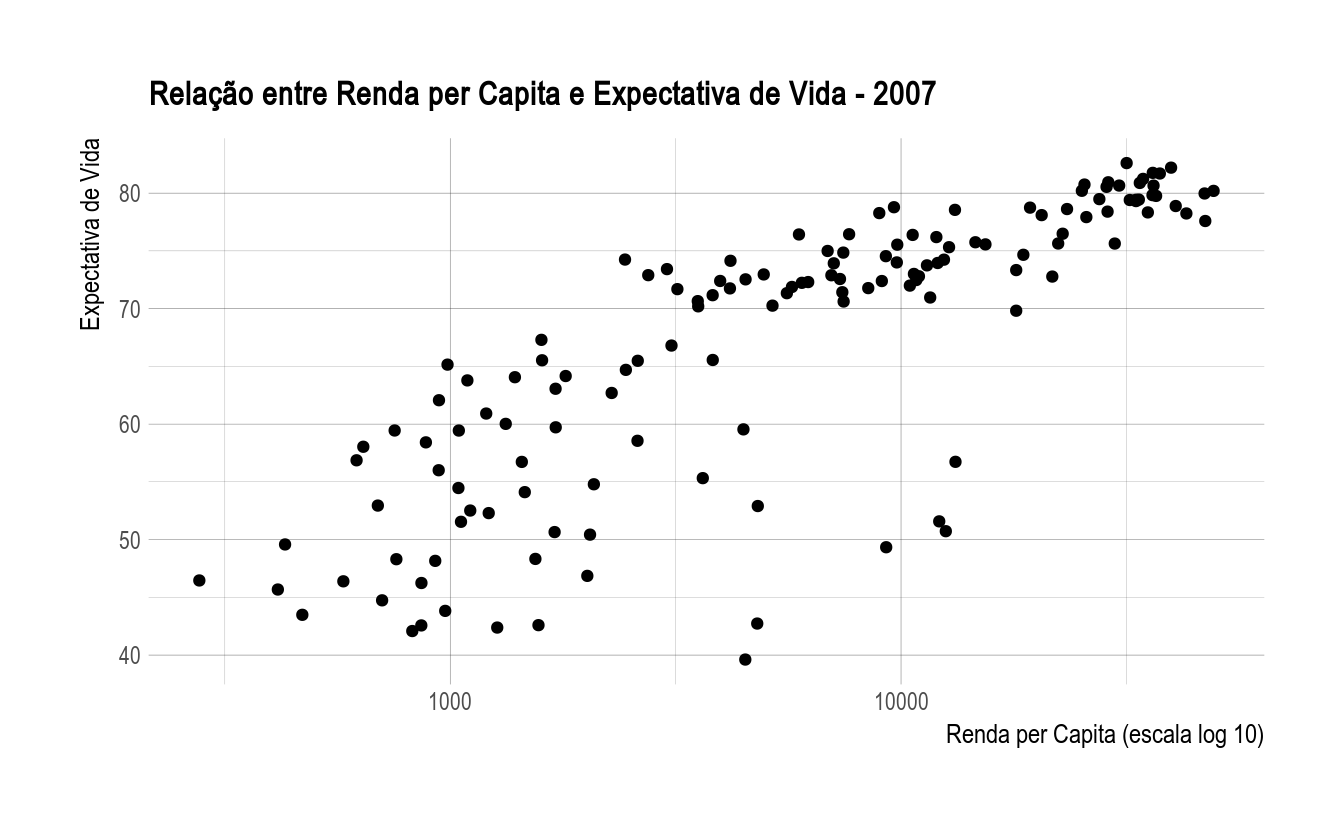
\includegraphics[width=1\linewidth]{bookdown-demo_files/figure-latex/unnamed-chunk-169-1} \end{center}

Note que a expectativa de vida cresce muito rápido para níveis de renda
baixos, mas o incremento decresce conforme o nível de renda aumenta.
Esse fato pode ser melhor representado utilizando uma escala logarítmica
para a variável renda per capita. É assim que usualmente essa relação é
apresentada. Para isso, poderíamos aplicar a função \texttt{log10()} na
variável de renda per capita, ou utilizar a função
\texttt{scale\_x\_log10()}:

\begin{Shaded}
\begin{Highlighting}[]
\NormalTok{gapminder }\OperatorTok\StringTok{ }
\StringTok{  }\KeywordTok{filter}\NormalTok{(year }\OperatorTok{==}\StringTok{ }\KeywordTok{max}\NormalTok{(year)) }\OperatorTok\StringTok{ }
\StringTok{  }\KeywordTok{ggplot}\NormalTok{(}\KeywordTok{aes}\NormalTok{(}\DataTypeTok{x =}\NormalTok{ gdpPercap, }\DataTypeTok{y =}\NormalTok{ lifeExp)) }\OperatorTok{+}
\StringTok{  }\KeywordTok{geom_point}\NormalTok{() }\OperatorTok{+}\StringTok{ }
\StringTok{  }\KeywordTok{scale_x_log10}\NormalTok{() }\OperatorTok{+}
\StringTok{  }\KeywordTok{labs}\NormalTok{(}\DataTypeTok{title =} \StringTok{"Relação entre Renda per Capita e Expectativa de Vida - 2007"}\NormalTok{,}
       \DataTypeTok{x =} \StringTok{"Renda per Capita (escala log 10)"}\NormalTok{,}
       \DataTypeTok{y =} \StringTok{"Expectativa de Vida"}\NormalTok{) }\OperatorTok{+}
\StringTok{  }\KeywordTok{theme_ipsum}\NormalTok{(}\DataTypeTok{plot_title_size =} \DecValTok{12}\NormalTok{,   }
              \DataTypeTok{axis_title_size =} \DecValTok{10}\NormalTok{)}
\end{Highlighting}
\end{Shaded}

\begin{center}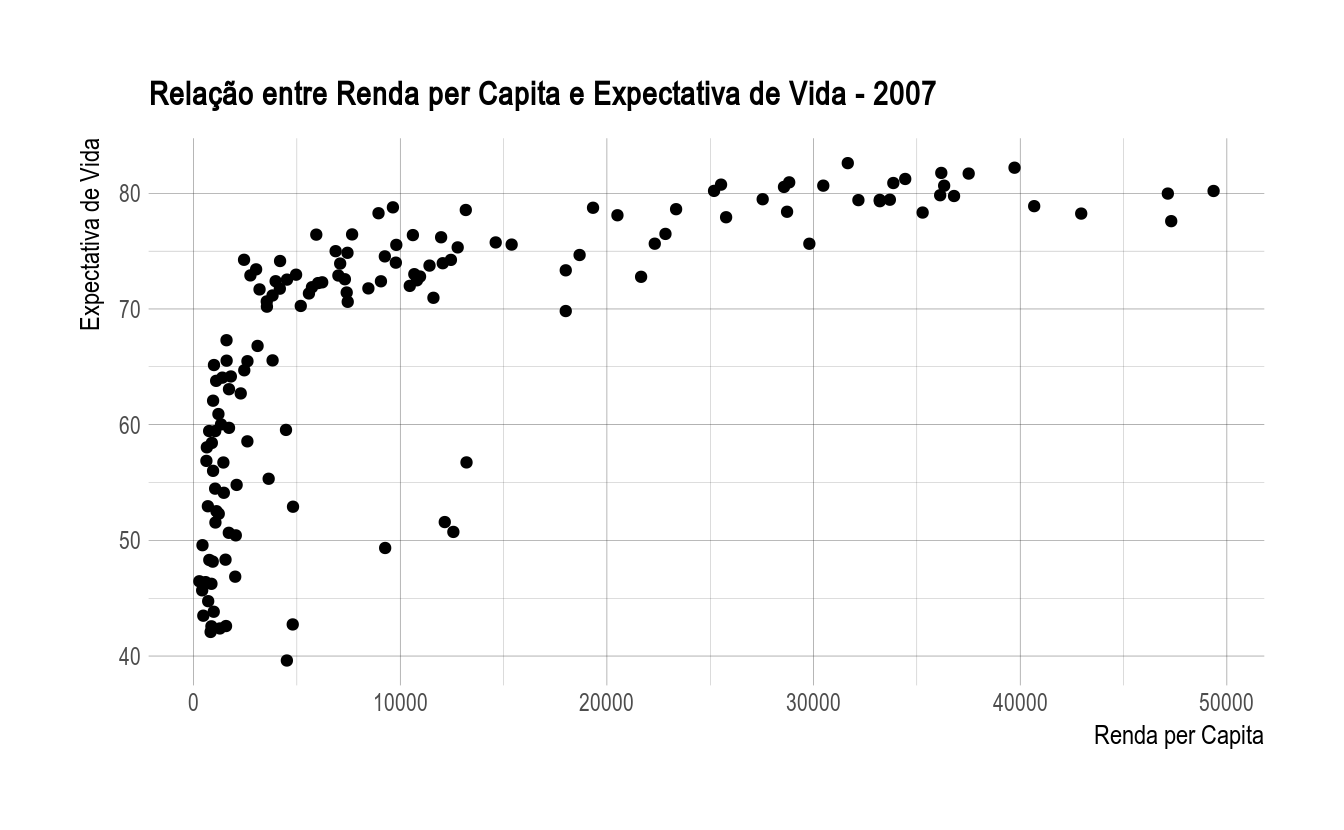
\includegraphics[width=1\linewidth]{bookdown-demo_files/figure-latex/unnamed-chunk-170-1} \end{center}

Com essa escala, valores incrementados na ordem de 10 vezes serão
igualmente espaçados. Nesse caso, a relação parece ser mais linear. Ou
seja, ao aumentar a renda 10 vezes, espera-se que a expectativa de vida
cresça a uma taxa constante.

Vamos mapear a variável \texttt{continent} ao elemento estético color e
shape:

\begin{Shaded}
\begin{Highlighting}[]
\NormalTok{gapminder }\OperatorTok\StringTok{ }
\StringTok{  }\KeywordTok{filter}\NormalTok{(year }\OperatorTok{==}\StringTok{ }\KeywordTok{max}\NormalTok{(year)) }\OperatorTok\StringTok{ }
\StringTok{  }\KeywordTok{ggplot}\NormalTok{(}\KeywordTok{aes}\NormalTok{(}\DataTypeTok{x =}\NormalTok{ gdpPercap, }\DataTypeTok{y =}\NormalTok{ lifeExp, }
             \DataTypeTok{color =}\NormalTok{ continent, }\DataTypeTok{shape =}\NormalTok{ continent)) }\OperatorTok{+}
\StringTok{  }\KeywordTok{geom_point}\NormalTok{() }\OperatorTok{+}\StringTok{ }
\StringTok{  }\KeywordTok{scale_x_log10}\NormalTok{() }\OperatorTok{+}
\StringTok{  }\KeywordTok{scale_color_discrete}\NormalTok{(}\StringTok{"Continente"}\NormalTok{) }\OperatorTok{+}
\StringTok{  }\KeywordTok{scale_shape_discrete}\NormalTok{(}\StringTok{"Continente"}\NormalTok{) }\OperatorTok{+}
\StringTok{  }\KeywordTok{labs}\NormalTok{(}\DataTypeTok{title =} \StringTok{"Relação entre Renda per Capita e Expectativa de Vida - 2007"}\NormalTok{,}
       \DataTypeTok{x =} \StringTok{"Renda per Capita (escala log 10)"}\NormalTok{,}
       \DataTypeTok{y =} \StringTok{"Expectativa de Vida"}\NormalTok{) }\OperatorTok{+}
\StringTok{  }\KeywordTok{theme_ipsum}\NormalTok{(}\DataTypeTok{plot_title_size =} \DecValTok{12}\NormalTok{,   }
              \DataTypeTok{axis_title_size =} \DecValTok{10}\NormalTok{)}
\end{Highlighting}
\end{Shaded}

\begin{center}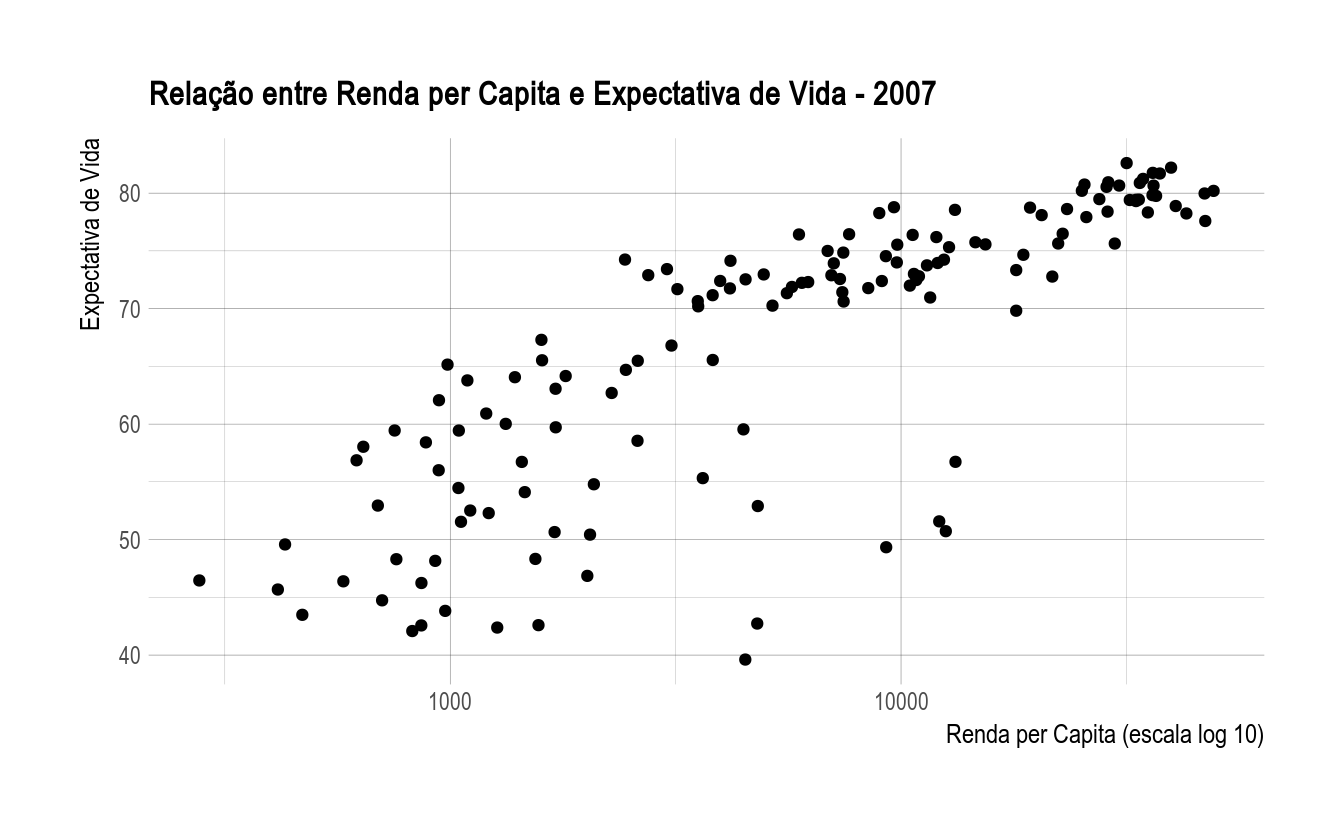
\includegraphics[width=1\linewidth]{bookdown-demo_files/figure-latex/unnamed-chunk-171-1} \end{center}

Automaticamente o ggplot2 criou uma escala para as cores e formatos dos
pontos. O usuário pode alterar esse mapeamento utilizando as funções
\texttt{scale\_*\_*}.

Por fim, fica aqui a lista com os tipos de shapes:

\begin{center}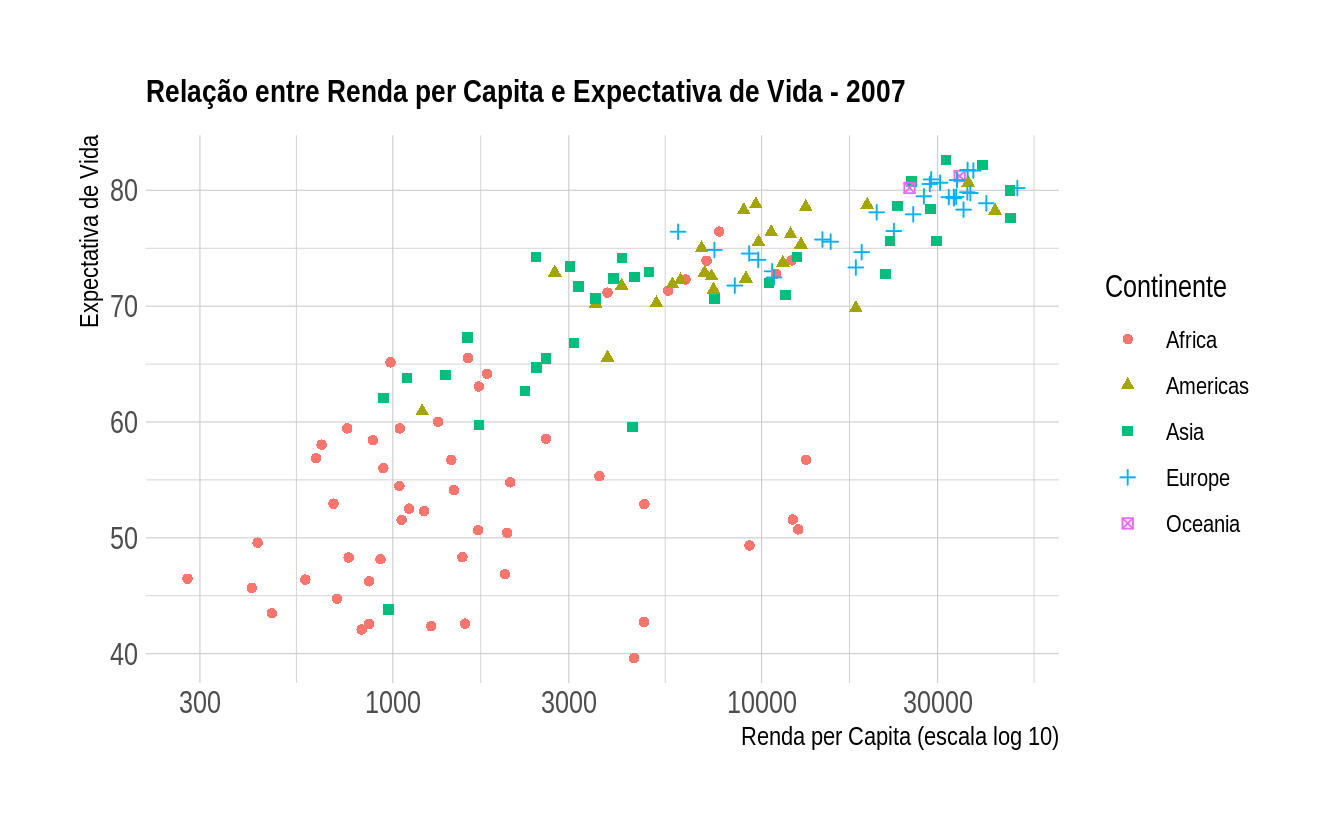
\includegraphics[width=1\linewidth]{bookdown-demo_files/figure-latex/unnamed-chunk-172-1} \end{center}

Perceba que os formatos de 21 a 24 possuem preenchimento
(\texttt{fill}). Assim, no código abaixo iremos definir o preenchimento,
o tamanho do ponto e a espessura para aqueles formatos que possuem
contornos.

\begin{Shaded}
\begin{Highlighting}[]
\NormalTok{gapminder }\OperatorTok\StringTok{ }
\StringTok{  }\KeywordTok{filter}\NormalTok{(year }\OperatorTok{==}\StringTok{ }\KeywordTok{max}\NormalTok{(year)) }\OperatorTok\StringTok{ }
\StringTok{  }\KeywordTok{ggplot}\NormalTok{(}\KeywordTok{aes}\NormalTok{(}\DataTypeTok{x =}\NormalTok{ gdpPercap, }\DataTypeTok{y =}\NormalTok{ lifeExp, }
             \DataTypeTok{color =}\NormalTok{ continent, }\DataTypeTok{shape =}\NormalTok{ continent)) }\OperatorTok{+}
\StringTok{  }\KeywordTok{geom_point}\NormalTok{(}\DataTypeTok{fill =} \StringTok{"black"}\NormalTok{, }\DataTypeTok{size =} \DecValTok{3}\NormalTok{, }\DataTypeTok{stroke =} \DecValTok{1}\NormalTok{) }\OperatorTok{+}\StringTok{ }
\StringTok{  }\KeywordTok{scale_x_log10}\NormalTok{() }\OperatorTok{+}
\StringTok{  }\KeywordTok{scale_color_discrete}\NormalTok{(}\StringTok{"Continente"}\NormalTok{) }\OperatorTok{+}
\StringTok{  }\KeywordTok{scale_shape_manual}\NormalTok{(}\StringTok{"Continente"}\NormalTok{, }\DataTypeTok{values =} \KeywordTok{c}\NormalTok{(}\DecValTok{19}\NormalTok{, }\DecValTok{21}\NormalTok{, }\DecValTok{22}\NormalTok{, }\DecValTok{23}\NormalTok{, }\DecValTok{24}\NormalTok{)) }\OperatorTok{+}
\StringTok{  }\KeywordTok{labs}\NormalTok{(}\DataTypeTok{title =} \StringTok{"Relação entre Renda per Capita e Expectativa de Vida - 2007"}\NormalTok{,}
       \DataTypeTok{x =} \StringTok{"Renda per Capita (escala log 10)"}\NormalTok{,}
       \DataTypeTok{y =} \StringTok{"Expectativa de Vida"}\NormalTok{)}
\end{Highlighting}
\end{Shaded}

\begin{center}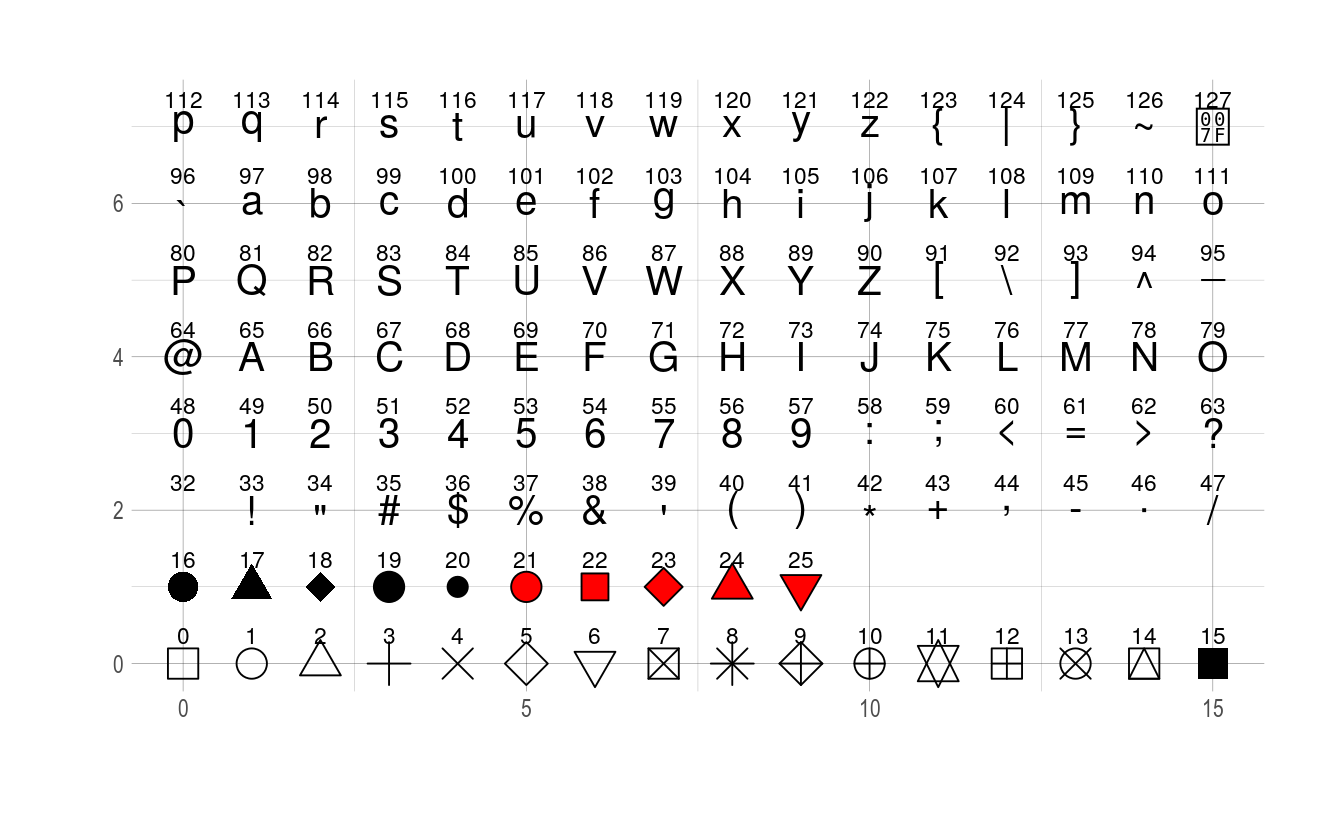
\includegraphics[width=1\linewidth]{bookdown-demo_files/figure-latex/unnamed-chunk-173-1} \end{center}

\section{Gráficos de Bolhas}\label{graficos-de-bolhas}

O gráfico de bolha é uma extensão natural do gráfico de pontos. Nele é
possível observar possíveis relações entre as três variáveis. Para esse
tipo de gráfico, são necessárias três variáveis. Duas para indicarem as
posições x e y, e uma terceira para definir o tamanho do ponto
(\texttt{size}). Vamos utilizar a variável \texttt{pop} (população):

\begin{Shaded}
\begin{Highlighting}[]
\NormalTok{gapminder }\OperatorTok\StringTok{ }
\StringTok{  }\KeywordTok{filter}\NormalTok{(year }\OperatorTok{==}\StringTok{ }\KeywordTok{max}\NormalTok{(year)) }\OperatorTok\StringTok{ }
\StringTok{  }\KeywordTok{ggplot}\NormalTok{(}\KeywordTok{aes}\NormalTok{(}\DataTypeTok{x =}\NormalTok{ gdpPercap, }\DataTypeTok{y =}\NormalTok{ lifeExp, }
             \DataTypeTok{size =}\NormalTok{ pop)) }\OperatorTok{+}
\StringTok{  }\KeywordTok{geom_point}\NormalTok{() }\OperatorTok{+}\StringTok{ }
\StringTok{  }\KeywordTok{scale_size_continuous}\NormalTok{(}\StringTok{"População (milhões)"}\NormalTok{, }\DataTypeTok{labels =} \ControlFlowTok{function}\NormalTok{(x) }\KeywordTok{round}\NormalTok{(x}\OperatorTok{/}\FloatTok{1e6}\NormalTok{)) }\OperatorTok{+}
\StringTok{  }\KeywordTok{scale_x_log10}\NormalTok{() }\OperatorTok{+}
\StringTok{  }\KeywordTok{labs}\NormalTok{(}\DataTypeTok{title =} \StringTok{"Relação entre Renda per Capita e Expectativa de Vida - 2007"}\NormalTok{,}
       \DataTypeTok{x =} \StringTok{"Renda per Capita (escala log 10)"}\NormalTok{,}
       \DataTypeTok{y =} \StringTok{"Expectativa de Vida"}\NormalTok{) }\OperatorTok{+}
\StringTok{  }\KeywordTok{theme_ipsum}\NormalTok{(}\DataTypeTok{plot_title_size =} \DecValTok{12}\NormalTok{,    }
              \DataTypeTok{axis_title_size =} \DecValTok{10}\NormalTok{)}
\end{Highlighting}
\end{Shaded}

\begin{center}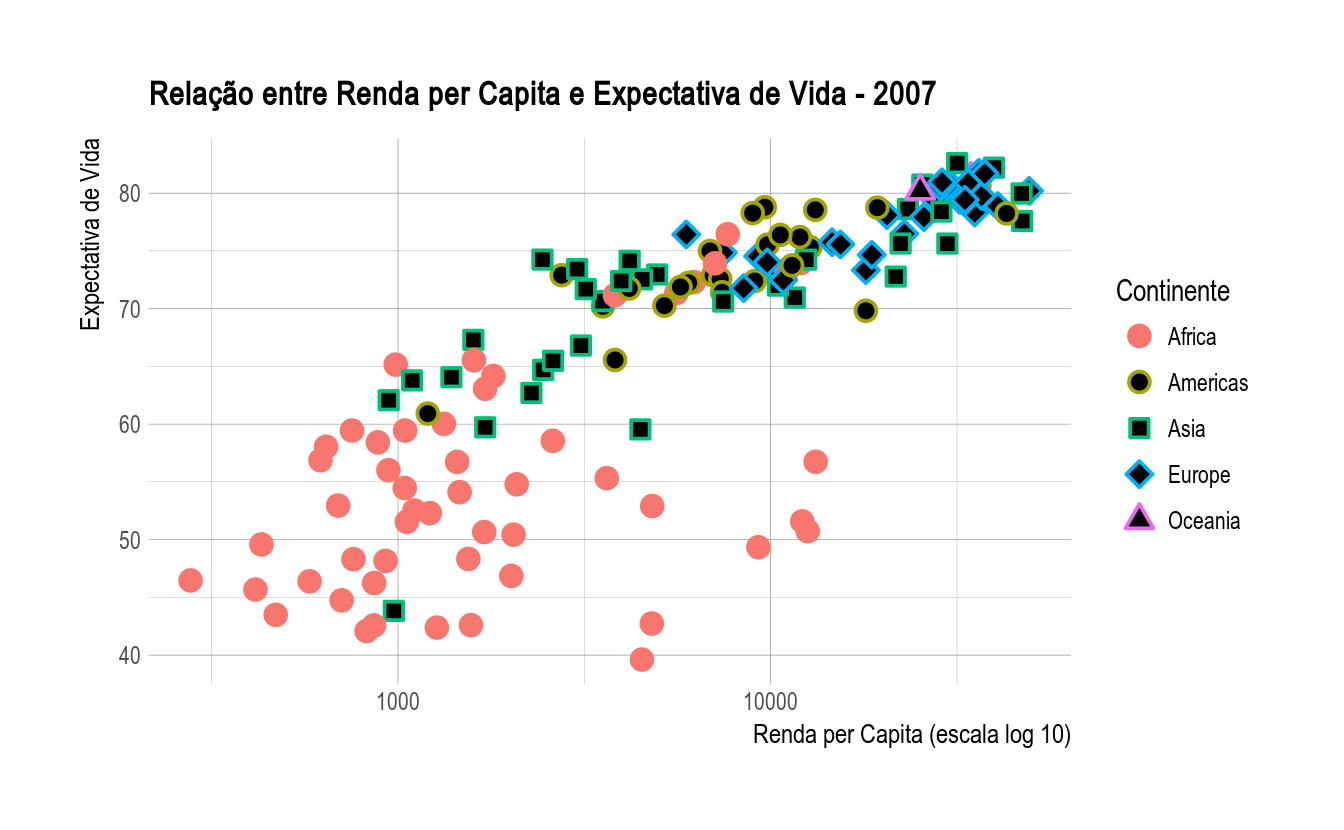
\includegraphics[width=1\linewidth]{bookdown-demo_files/figure-latex/unnamed-chunk-174-1} \end{center}

\section{Gráficos de Barras}\label{graficos-de-barras}

Os gráficos de barras/colunas são geralmente utilizados para comparações
entre categorias (variáveis qualitativas). No ggplot2, podemos usar dois
objetos geométricos distintos:

\begin{Shaded}
\begin{Highlighting}[]
\KeywordTok{geom_bar}\NormalTok{(}\DataTypeTok{mapping =} \OtherTok{NULL}\NormalTok{, }\DataTypeTok{data =} \OtherTok{NULL}\NormalTok{, }\DataTypeTok{stat =} \StringTok{"count"}\NormalTok{, }\DataTypeTok{position =} \StringTok{"stack"}\NormalTok{, ...,}
         \DataTypeTok{width =} \OtherTok{NULL}\NormalTok{, }\DataTypeTok{binwidth =} \OtherTok{NULL}\NormalTok{, }\DataTypeTok{na.rm =} \OtherTok{FALSE}\NormalTok{, }\DataTypeTok{show.legend =} \OtherTok{NA}\NormalTok{,}
         \DataTypeTok{inherit.aes =} \OtherTok{TRUE}\NormalTok{)}

\KeywordTok{geom_col}\NormalTok{(}\DataTypeTok{mapping =} \OtherTok{NULL}\NormalTok{, }\DataTypeTok{data =} \OtherTok{NULL}\NormalTok{, }\DataTypeTok{position =} \StringTok{"stack"}\NormalTok{, ...,}
  \DataTypeTok{width =} \OtherTok{NULL}\NormalTok{, }\DataTypeTok{na.rm =} \OtherTok{FALSE}\NormalTok{, }\DataTypeTok{show.legend =} \OtherTok{NA}\NormalTok{, }\DataTypeTok{inherit.aes =} \OtherTok{TRUE}\NormalTok{)}
\end{Highlighting}
\end{Shaded}

Os parâmetros estéticos (aes) são:

\begin{itemize}
\tightlist
\item
  \textbf{\texttt{x}}
\item
  \texttt{y} (somente com \texttt{stat=identity})
\item
  \texttt{alpha}
\item
  \texttt{colour}
\item
  \texttt{fill}
\item
  \texttt{linetype}
\item
  \texttt{size}
\end{itemize}

Há um detalhe importante para o \texttt{geom\_bar()}, o argumento
\texttt{stat}. Por padrão, para esse objeto geométrico, o valor de
\texttt{stat} é \texttt{count}, o que significa que ele irá fazer uma
contagem dos elementos dos eixo x. Essa contagem será usada no eixo
\texttt{y}. Por exemplo:

\begin{Shaded}
\begin{Highlighting}[]
\KeywordTok{ggplot}\NormalTok{(diamonds, }\KeywordTok{aes}\NormalTok{(}\DataTypeTok{x =}\NormalTok{ cut)) }\OperatorTok{+}
\StringTok{  }\KeywordTok{geom_bar}\NormalTok{() }\OperatorTok{+}
\StringTok{  }\KeywordTok{theme_ipsum}\NormalTok{(}\DataTypeTok{plot_title_size =} \DecValTok{12}\NormalTok{,   }
              \DataTypeTok{axis_title_size =} \DecValTok{10}\NormalTok{)}
\end{Highlighting}
\end{Shaded}

\begin{center}\includegraphics[width=1\linewidth]{bookdown-demo_files/figure-latex/unnamed-chunk-176-1} \end{center}

Para cada valor da variável \texttt{cut}, o ggplot2 calculou o número de
observações no data.frame \texttt{diamonds}.

Para que o \texttt{y} seja mapeado para uma variável do data.frame, é
necessário definir \texttt{stat\ =\ identity}.

\begin{Shaded}
\begin{Highlighting}[]
\NormalTok{gapminder }\OperatorTok\StringTok{ }
\StringTok{  }\KeywordTok{filter}\NormalTok{(year }\OperatorTok{==}\StringTok{ }\KeywordTok{max}\NormalTok{(year),}
\NormalTok{         continent }\OperatorTok{==}\StringTok{ "Americas"}\NormalTok{) }\OperatorTok\StringTok{ }
\StringTok{  }\KeywordTok{ggplot}\NormalTok{(}\KeywordTok{aes}\NormalTok{(}\DataTypeTok{x =}\NormalTok{ country, }\DataTypeTok{y =}\NormalTok{ lifeExp)) }\OperatorTok{+}
\StringTok{  }\KeywordTok{geom_bar}\NormalTok{(}\DataTypeTok{stat =} \StringTok{"identity"}\NormalTok{, }\DataTypeTok{fill =} \StringTok{"dodgerblue"}\NormalTok{) }\OperatorTok{+}
\StringTok{  }\KeywordTok{labs}\NormalTok{(}\DataTypeTok{title =} \StringTok{"Expectativa de vida por país"}\NormalTok{,}
       \DataTypeTok{subtitle =} \StringTok{"2007"}\NormalTok{,}
       \DataTypeTok{x =} \StringTok{"País"}\NormalTok{,}
       \DataTypeTok{y =} \StringTok{"Expectativa de Vida"}\NormalTok{) }\OperatorTok{+}
\StringTok{  }\KeywordTok{theme}\NormalTok{(}\DataTypeTok{axis.text.x =} \KeywordTok{element_text}\NormalTok{(}\DataTypeTok{angle =} \DecValTok{90}\NormalTok{, }\DataTypeTok{hjust =} \DecValTok{1}\NormalTok{))}
\end{Highlighting}
\end{Shaded}

\begin{center}\includegraphics[width=1\linewidth]{bookdown-demo_files/figure-latex/unnamed-chunk-177-1} \end{center}

Usando o \texttt{geom\_col()}:

\begin{Shaded}
\begin{Highlighting}[]
\NormalTok{gapminder }\OperatorTok\StringTok{ }
\StringTok{  }\KeywordTok{filter}\NormalTok{(year }\OperatorTok{==}\StringTok{ }\KeywordTok{max}\NormalTok{(year),}
\NormalTok{         continent }\OperatorTok{==}\StringTok{ "Americas"}\NormalTok{) }\OperatorTok\StringTok{ }
\StringTok{  }\KeywordTok{ggplot}\NormalTok{(}\KeywordTok{aes}\NormalTok{(}\DataTypeTok{x =}\NormalTok{ country, }\DataTypeTok{y =}\NormalTok{ lifeExp)) }\OperatorTok{+}
\StringTok{  }\KeywordTok{geom_col}\NormalTok{(}\DataTypeTok{fill =} \StringTok{"dodgerblue"}\NormalTok{) }\OperatorTok{+}
\StringTok{  }\KeywordTok{labs}\NormalTok{(}\DataTypeTok{title =} \StringTok{"Expectativa de vida por país"}\NormalTok{,}
       \DataTypeTok{subtitle =} \StringTok{"2007"}\NormalTok{,}
       \DataTypeTok{x =} \StringTok{"País"}\NormalTok{,}
       \DataTypeTok{y =} \StringTok{"Anos"}\NormalTok{) }\OperatorTok{+}
\StringTok{  }\KeywordTok{theme}\NormalTok{(}\DataTypeTok{axis.text.x =} \KeywordTok{element_text}\NormalTok{(}\DataTypeTok{angle =} \DecValTok{90}\NormalTok{, }\DataTypeTok{hjust =} \DecValTok{1}\NormalTok{))}
\end{Highlighting}
\end{Shaded}

\begin{center}\includegraphics[width=1\linewidth]{bookdown-demo_files/figure-latex/unnamed-chunk-178-1} \end{center}

Uma pergunta recorrente é: Como ordenar as barras em ordem
crescente/decrescente? Para isso, pode-se usar a função
\texttt{reorder()} no momento do mapeamento. Fica mais claro com um
exemplo:

\begin{Shaded}
\begin{Highlighting}[]
\NormalTok{gapminder }\OperatorTok\StringTok{ }
\StringTok{  }\KeywordTok{filter}\NormalTok{(year }\OperatorTok{==}\StringTok{ }\KeywordTok{max}\NormalTok{(year),}
\NormalTok{         continent }\OperatorTok{==}\StringTok{ "Americas"}\NormalTok{) }\OperatorTok\StringTok{ }
\StringTok{  }\KeywordTok{ggplot}\NormalTok{(}\KeywordTok{aes}\NormalTok{(}\DataTypeTok{x =} \KeywordTok{reorder}\NormalTok{(country, }\OperatorTok{-}\NormalTok{lifeExp), }\DataTypeTok{y =}\NormalTok{ lifeExp)) }\OperatorTok{+}
\StringTok{  }\KeywordTok{geom_col}\NormalTok{(}\DataTypeTok{fill =} \StringTok{"dodgerblue"}\NormalTok{) }\OperatorTok{+}
\StringTok{  }\KeywordTok{labs}\NormalTok{(}\DataTypeTok{title =} \StringTok{"Expectativa de vida por país"}\NormalTok{,}
       \DataTypeTok{subtitle =} \StringTok{"2007"}\NormalTok{,}
       \DataTypeTok{x =} \StringTok{"País"}\NormalTok{,}
       \DataTypeTok{y =} \StringTok{"Anos"}\NormalTok{) }\OperatorTok{+}
\StringTok{  }\KeywordTok{theme}\NormalTok{(}\DataTypeTok{axis.text.x =} \KeywordTok{element_text}\NormalTok{(}\DataTypeTok{angle =} \DecValTok{90}\NormalTok{, }\DataTypeTok{hjust =} \DecValTok{1}\NormalTok{))}
\end{Highlighting}
\end{Shaded}

\begin{center}\includegraphics[width=1\linewidth]{bookdown-demo_files/figure-latex/unnamed-chunk-179-1} \end{center}

Vamos agora criar um gráfico em que se compara a expectativa de vida
média por continente em 1957 e 2007:

\begin{Shaded}
\begin{Highlighting}[]
\NormalTok{gapminder }\OperatorTok\StringTok{ }
\StringTok{  }\KeywordTok{filter}\NormalTok{(year }\OperatorTok\StringTok{ }\KeywordTok{c}\NormalTok{(}\DecValTok{1957}\NormalTok{, }\DecValTok{2007}\NormalTok{)) }\OperatorTok\StringTok{ }
\StringTok{  }\CommentTok{# Converte o ano para factor - será categoria no gráfico}
\StringTok{  }\KeywordTok{mutate}\NormalTok{(}\DataTypeTok{year =} \KeywordTok{factor}\NormalTok{(year)) }\OperatorTok\StringTok{ }
\StringTok{  }\KeywordTok{group_by}\NormalTok{(continent, year) }\OperatorTok\StringTok{ }
\StringTok{  }\KeywordTok{summarise}\NormalTok{(}\DataTypeTok{lifeExp =} \KeywordTok{mean}\NormalTok{(lifeExp)) }\OperatorTok\StringTok{ }
\StringTok{  }\KeywordTok{ggplot}\NormalTok{(}\KeywordTok{aes}\NormalTok{(}\DataTypeTok{x =}\NormalTok{ continent, }\DataTypeTok{y =}\NormalTok{ lifeExp, }\DataTypeTok{fill =}\NormalTok{ year)) }\OperatorTok{+}
\StringTok{  }\KeywordTok{geom_col}\NormalTok{() }\OperatorTok{+}
\StringTok{  }\KeywordTok{theme_ipsum}\NormalTok{(}\DataTypeTok{plot_title_size =} \DecValTok{12}\NormalTok{,   }
              \DataTypeTok{axis_title_size =} \DecValTok{10}\NormalTok{)}
\end{Highlighting}
\end{Shaded}

\begin{center}\includegraphics[width=1\linewidth]{bookdown-demo_files/figure-latex/unnamed-chunk-180-1} \end{center}

Para continente, o gráfico empilhou as barras. Isto se deve ao argumento
\texttt{position\ =\ stack}. Para colocar as barras lado a lado,
utilizamos o valor ``dodge'':

\begin{Shaded}
\begin{Highlighting}[]
\NormalTok{gapminder }\OperatorTok\StringTok{ }
\StringTok{  }\KeywordTok{filter}\NormalTok{(year }\OperatorTok\StringTok{ }\KeywordTok{c}\NormalTok{(}\DecValTok{1957}\NormalTok{, }\DecValTok{2007}\NormalTok{)) }\OperatorTok\StringTok{ }
\StringTok{  }\CommentTok{# Converte o ano para factor - será categoria no gráfico}
\StringTok{  }\KeywordTok{mutate}\NormalTok{(}\DataTypeTok{year =} \KeywordTok{factor}\NormalTok{(year)) }\OperatorTok\StringTok{ }
\StringTok{  }\KeywordTok{group_by}\NormalTok{(continent, year) }\OperatorTok\StringTok{ }
\StringTok{  }\KeywordTok{summarise}\NormalTok{(}\DataTypeTok{lifeExp =} \KeywordTok{mean}\NormalTok{(lifeExp)) }\OperatorTok\StringTok{ }
\StringTok{  }\KeywordTok{ggplot}\NormalTok{(}\KeywordTok{aes}\NormalTok{(}\DataTypeTok{x =}\NormalTok{ continent, }\DataTypeTok{y =}\NormalTok{ lifeExp, }\DataTypeTok{fill =}\NormalTok{ year)) }\OperatorTok{+}
\StringTok{  }\KeywordTok{geom_col}\NormalTok{(}\DataTypeTok{position =} \StringTok{"dodge"}\NormalTok{) }\OperatorTok{+}
\StringTok{  }\KeywordTok{labs}\NormalTok{(}\DataTypeTok{title =} \StringTok{"Expectativa de vida por continente"}\NormalTok{,}
       \DataTypeTok{x =} \StringTok{"Continente"}\NormalTok{,}
       \DataTypeTok{y =} \StringTok{"Anos"}\NormalTok{,}
       \DataTypeTok{fill =} \StringTok{"Ano"}\NormalTok{) }\OperatorTok{+}
\StringTok{  }\KeywordTok{theme_ipsum}\NormalTok{(}\DataTypeTok{plot_title_size =} \DecValTok{12}\NormalTok{, }
              \DataTypeTok{axis_title_size =} \DecValTok{10}\NormalTok{)}
\end{Highlighting}
\end{Shaded}

\begin{center}\includegraphics[width=1\linewidth]{bookdown-demo_files/figure-latex/unnamed-chunk-181-1} \end{center}

Também é comum representar as barras horizontalmente. Basta usar a
função \texttt{coord\_flip()}:

\begin{Shaded}
\begin{Highlighting}[]
\NormalTok{gapminder }\OperatorTok\StringTok{ }
\StringTok{  }\KeywordTok{filter}\NormalTok{(year }\OperatorTok\StringTok{ }\KeywordTok{c}\NormalTok{(}\DecValTok{1957}\NormalTok{, }\DecValTok{2007}\NormalTok{)) }\OperatorTok\StringTok{ }
\StringTok{  }\CommentTok{# Converte o ano para factor - será categoria no gráfico}
\StringTok{  }\KeywordTok{mutate}\NormalTok{(}\DataTypeTok{year =} \KeywordTok{factor}\NormalTok{(year)) }\OperatorTok\StringTok{ }
\StringTok{  }\KeywordTok{group_by}\NormalTok{(continent, year) }\OperatorTok\StringTok{ }
\StringTok{  }\KeywordTok{summarise}\NormalTok{(}\DataTypeTok{lifeExp =} \KeywordTok{mean}\NormalTok{(lifeExp)) }\OperatorTok\StringTok{ }
\StringTok{  }\KeywordTok{ggplot}\NormalTok{(}\KeywordTok{aes}\NormalTok{(}\DataTypeTok{x =}\NormalTok{ continent, }\DataTypeTok{y =}\NormalTok{ lifeExp, }\DataTypeTok{fill =}\NormalTok{ year)) }\OperatorTok{+}
\StringTok{  }\KeywordTok{geom_col}\NormalTok{(}\DataTypeTok{position =} \StringTok{"dodge"}\NormalTok{) }\OperatorTok{+}
\StringTok{  }\KeywordTok{coord_flip}\NormalTok{() }\OperatorTok{+}
\StringTok{  }\KeywordTok{labs}\NormalTok{(}\DataTypeTok{title =} \StringTok{"Expectativa de vida por continente"}\NormalTok{,}
       \DataTypeTok{x =} \StringTok{"Continente"}\NormalTok{,}
       \DataTypeTok{y =} \StringTok{"Anos"}\NormalTok{,}
       \DataTypeTok{fill =} \StringTok{"Ano"}\NormalTok{) }\OperatorTok{+}
\StringTok{  }\KeywordTok{theme_ipsum}\NormalTok{(}\DataTypeTok{plot_title_size =} \DecValTok{12}\NormalTok{, }
              \DataTypeTok{axis_title_size =} \DecValTok{10}\NormalTok{)}
\end{Highlighting}
\end{Shaded}

\begin{center}\includegraphics[width=1\linewidth]{bookdown-demo_files/figure-latex/unnamed-chunk-182-1} \end{center}

\section{Gráficos de linhas}\label{graficos-de-linhas}

Os gráficos de linhas são geralmente utilizados para apresentar a
evolução de uma variável quantitativa em um intervalo de tempo.

\begin{Shaded}
\begin{Highlighting}[]
\KeywordTok{geom_line}\NormalTok{(}\DataTypeTok{mapping =} \OtherTok{NULL}\NormalTok{, }\DataTypeTok{data =} \OtherTok{NULL}\NormalTok{, }\DataTypeTok{stat =} \StringTok{"identity"}\NormalTok{, }\DataTypeTok{position =} \StringTok{"identity"}\NormalTok{,}
          \DataTypeTok{na.rm =} \OtherTok{FALSE}\NormalTok{, }\DataTypeTok{show.legend =} \OtherTok{NA}\NormalTok{, }\DataTypeTok{inherit.aes =} \OtherTok{TRUE}\NormalTok{, ...)}
\end{Highlighting}
\end{Shaded}

Os parâmetros estéticos (aes) são:

\begin{itemize}
\tightlist
\item
  \textbf{\texttt{x}}
\item
  \textbf{\texttt{y}}
\item
  \texttt{alpha}
\item
  \texttt{colour}
\item
  \texttt{linetype}
\item
  \texttt{size}
\end{itemize}

\begin{Shaded}
\begin{Highlighting}[]
\NormalTok{gapminder }\OperatorTok\StringTok{ }
\StringTok{  }\KeywordTok{group_by}\NormalTok{(continent, year) }\OperatorTok\StringTok{ }
\StringTok{  }\KeywordTok{summarise}\NormalTok{(}\DataTypeTok{lifeExp =} \KeywordTok{mean}\NormalTok{(lifeExp)) }\OperatorTok\StringTok{ }
\StringTok{  }\KeywordTok{ggplot}\NormalTok{(}\KeywordTok{aes}\NormalTok{(}\DataTypeTok{x =}\NormalTok{ year, }\DataTypeTok{y =}\NormalTok{ lifeExp, }\DataTypeTok{color =}\NormalTok{ continent)) }\OperatorTok{+}
\StringTok{  }\KeywordTok{geom_line}\NormalTok{() }\OperatorTok{+}
\StringTok{  }\KeywordTok{labs}\NormalTok{(}\DataTypeTok{title =} \StringTok{"Evolução da expectativa de vida por continente"}\NormalTok{,}
       \DataTypeTok{x =} \StringTok{"Ano"}\NormalTok{,}
       \DataTypeTok{y =} \StringTok{"Anos de vida"}\NormalTok{,}
       \DataTypeTok{color =} \StringTok{"Continente"}\NormalTok{) }\OperatorTok{+}
\StringTok{  }\KeywordTok{theme_ipsum}\NormalTok{(}\DataTypeTok{plot_title_size =} \DecValTok{12}\NormalTok{,   }
              \DataTypeTok{axis_title_size =} \DecValTok{10}\NormalTok{)}
\end{Highlighting}
\end{Shaded}

\begin{center}\includegraphics[width=1\linewidth]{bookdown-demo_files/figure-latex/unnamed-chunk-184-1} \end{center}

É bastante comum que gráficos de linhas apresentem marcações para os
períodos em que realmente existem os dados. Para isso, podemos adicionar
uma camada de pontos:

\begin{Shaded}
\begin{Highlighting}[]
\NormalTok{gapminder }\OperatorTok\StringTok{ }
\StringTok{  }\KeywordTok{group_by}\NormalTok{(continent, year) }\OperatorTok\StringTok{ }
\StringTok{  }\KeywordTok{summarise}\NormalTok{(}\DataTypeTok{lifeExp =} \KeywordTok{mean}\NormalTok{(lifeExp)) }\OperatorTok\StringTok{ }
\StringTok{  }\KeywordTok{ggplot}\NormalTok{(}\KeywordTok{aes}\NormalTok{(}\DataTypeTok{x =}\NormalTok{ year, }\DataTypeTok{y =}\NormalTok{ lifeExp, }\DataTypeTok{color =}\NormalTok{ continent)) }\OperatorTok{+}
\StringTok{  }\KeywordTok{geom_line}\NormalTok{() }\OperatorTok{+}
\StringTok{  }\KeywordTok{geom_point}\NormalTok{(}\KeywordTok{aes}\NormalTok{(}\DataTypeTok{shape =}\NormalTok{ continent)) }\OperatorTok{+}
\StringTok{  }\KeywordTok{labs}\NormalTok{(}\DataTypeTok{title =} \StringTok{"Evolução da expectativa de vida por continente"}\NormalTok{,}
       \DataTypeTok{x =} \StringTok{"Ano"}\NormalTok{,}
       \DataTypeTok{y =} \StringTok{"Anos de vida"}\NormalTok{,}
       \DataTypeTok{color =} \StringTok{"Continente"}\NormalTok{,}
       \DataTypeTok{shape =} \StringTok{"Continente"}\NormalTok{) }\OperatorTok{+}
\StringTok{  }\KeywordTok{theme_ipsum}\NormalTok{(}\DataTypeTok{plot_title_size =} \DecValTok{12}\NormalTok{,    }
              \DataTypeTok{axis_title_size =} \DecValTok{10}\NormalTok{)}
\end{Highlighting}
\end{Shaded}

\begin{center}\includegraphics[width=1\linewidth]{bookdown-demo_files/figure-latex/unnamed-chunk-185-1} \end{center}

\section{Histogramas e freqpoly}\label{histogramas-e-freqpoly}

\begin{Shaded}
\begin{Highlighting}[]
\KeywordTok{geom_freqpoly}\NormalTok{(}\DataTypeTok{mapping =} \OtherTok{NULL}\NormalTok{, }\DataTypeTok{data =} \OtherTok{NULL}\NormalTok{, }\DataTypeTok{stat =} \StringTok{"bin"}\NormalTok{,}
  \DataTypeTok{position =} \StringTok{"identity"}\NormalTok{, ..., }\DataTypeTok{na.rm =} \OtherTok{FALSE}\NormalTok{, }\DataTypeTok{show.legend =} \OtherTok{NA}\NormalTok{,}
  \DataTypeTok{inherit.aes =} \OtherTok{TRUE}\NormalTok{)}

\KeywordTok{geom_histogram}\NormalTok{(}\DataTypeTok{mapping =} \OtherTok{NULL}\NormalTok{, }\DataTypeTok{data =} \OtherTok{NULL}\NormalTok{, }\DataTypeTok{stat =} \StringTok{"bin"}\NormalTok{,}
  \DataTypeTok{position =} \StringTok{"stack"}\NormalTok{, ..., }\DataTypeTok{binwidth =} \OtherTok{NULL}\NormalTok{, }\DataTypeTok{bins =} \OtherTok{NULL}\NormalTok{, }\DataTypeTok{na.rm =} \OtherTok{FALSE}\NormalTok{,}
  \DataTypeTok{show.legend =} \OtherTok{NA}\NormalTok{, }\DataTypeTok{inherit.aes =} \OtherTok{TRUE}\NormalTok{)}
\end{Highlighting}
\end{Shaded}

Os histogramas são utilizados para representar a distribuição de dados
de uma variável quantitativa em intervalos contínuos. Esses intervalos
são chamados de \texttt{bins}. Para cada bin, será apresentado a
quantidade de valores que estão naquele intervalo. A diferença para o
\texttt{geom\_freqpoly} é que este utiliza linhas para construir
polígonos, enquanto o \texttt{geom\_histogram} utiliza barras.

Conforme a documentação do ggplot2, o \texttt{geom\_histogram()} utiliza
os mesmos elementos estéticos do \texttt{geom\_bar()}. Já o
\texttt{geom\_freqpoly()} utiliza os mesmo do \texttt{geom\_line()}.

\begin{Shaded}
\begin{Highlighting}[]
\NormalTok{gapminder }\OperatorTok\StringTok{ }
\StringTok{  }\KeywordTok{filter}\NormalTok{(year }\OperatorTok{==}\StringTok{ }\DecValTok{2007}\NormalTok{) }\OperatorTok\StringTok{ }
\StringTok{  }\KeywordTok{ggplot}\NormalTok{(}\KeywordTok{aes}\NormalTok{(}\DataTypeTok{x =}\NormalTok{ lifeExp)) }\OperatorTok{+}
\StringTok{  }\KeywordTok{geom_histogram}\NormalTok{(}\DataTypeTok{binwidth =} \DecValTok{5}\NormalTok{, }\DataTypeTok{fill =} \StringTok{'dodgerblue'}\NormalTok{, }\DataTypeTok{color =} \StringTok{'black'}\NormalTok{) }\OperatorTok{+}
\StringTok{  }\KeywordTok{labs}\NormalTok{(}\DataTypeTok{title =} \StringTok{"Distribuição da expectativa vida"}\NormalTok{,}
       \DataTypeTok{x =} \StringTok{"Anos"}\NormalTok{,}
       \DataTypeTok{y =} \StringTok{"Contagem"}\NormalTok{) }\OperatorTok{+}
\StringTok{  }\KeywordTok{theme_ipsum}\NormalTok{(}\DataTypeTok{plot_title_size =} \DecValTok{12}\NormalTok{,   }
              \DataTypeTok{axis_title_size =} \DecValTok{10}\NormalTok{)}
\end{Highlighting}
\end{Shaded}

\begin{center}\includegraphics[width=1\linewidth]{bookdown-demo_files/figure-latex/unnamed-chunk-187-1} \end{center}

\begin{Shaded}
\begin{Highlighting}[]
\NormalTok{gapminder }\OperatorTok\StringTok{ }
\StringTok{  }\KeywordTok{filter}\NormalTok{(year }\OperatorTok{==}\StringTok{ }\DecValTok{2007}\NormalTok{) }\OperatorTok\StringTok{ }
\StringTok{  }\KeywordTok{ggplot}\NormalTok{(}\KeywordTok{aes}\NormalTok{(}\DataTypeTok{x =}\NormalTok{ lifeExp)) }\OperatorTok{+}
\StringTok{  }\KeywordTok{geom_freqpoly}\NormalTok{(}\DataTypeTok{binwidth =} \DecValTok{5}\NormalTok{) }\OperatorTok{+}
\StringTok{  }\KeywordTok{labs}\NormalTok{(}\DataTypeTok{title =} \StringTok{"Distribuição da expectativa vida"}\NormalTok{,}
       \DataTypeTok{x =} \StringTok{"Anos"}\NormalTok{,}
       \DataTypeTok{y =} \StringTok{"Contagem"}\NormalTok{) }\OperatorTok{+}
\StringTok{  }\KeywordTok{theme_ipsum}\NormalTok{(}\DataTypeTok{plot_title_size =} \DecValTok{12}\NormalTok{,     }
              \DataTypeTok{axis_title_size =} \DecValTok{10}\NormalTok{)}
\end{Highlighting}
\end{Shaded}

\begin{center}\includegraphics[width=1\linewidth]{bookdown-demo_files/figure-latex/unnamed-chunk-188-1} \end{center}

Transformando em proporção:

\begin{Shaded}
\begin{Highlighting}[]
\NormalTok{gapminder }\OperatorTok\StringTok{ }
\StringTok{  }\KeywordTok{filter}\NormalTok{(year }\OperatorTok{==}\StringTok{ }\DecValTok{2007}\NormalTok{) }\OperatorTok\StringTok{ }
\StringTok{  }\KeywordTok{ggplot}\NormalTok{(}\KeywordTok{aes}\NormalTok{(}\DataTypeTok{x =}\NormalTok{ lifeExp)) }\OperatorTok{+}
\StringTok{  }\KeywordTok{geom_histogram}\NormalTok{(}\KeywordTok{aes}\NormalTok{(}\DataTypeTok{y =}\NormalTok{ ..count..}\OperatorTok{/}\KeywordTok{sum}\NormalTok{(..count..)),}\DataTypeTok{binwidth =} \DecValTok{5}\NormalTok{, }\DataTypeTok{fill =} \StringTok{'dodgerblue'}\NormalTok{, }\DataTypeTok{color =} \StringTok{'black'}\NormalTok{) }\OperatorTok{+}
\StringTok{  }\KeywordTok{labs}\NormalTok{(}\DataTypeTok{title =} \StringTok{"Distribuição da expectativa vida"}\NormalTok{,}
       \DataTypeTok{x =} \StringTok{"Anos"}\NormalTok{,}
       \DataTypeTok{y =} \StringTok{"Proporção"}\NormalTok{) }\OperatorTok{+}
\StringTok{  }\KeywordTok{scale_y_continuous}\NormalTok{(}\DataTypeTok{labels =}\NormalTok{ scales}\OperatorTok{::}\KeywordTok{percent_format}\NormalTok{()) }\OperatorTok{+}
\StringTok{  }\KeywordTok{theme_ipsum}\NormalTok{(}\DataTypeTok{plot_title_size =} \DecValTok{12}\NormalTok{,}
              \DataTypeTok{axis_title_size =} \DecValTok{10}\NormalTok{)}
\end{Highlighting}
\end{Shaded}

\begin{center}\includegraphics[width=1\linewidth]{bookdown-demo_files/figure-latex/unnamed-chunk-189-1} \end{center}

O ggplot2 internamente criou a variável \texttt{..count..}. Dessa forma,
podemos utilizá-la para criar as proporções.

\section{Boxplots, jitterplots e
violinplots}\label{boxplots-jitterplots-e-violinplots}

O boxplot é uma representação comum para apresentar a distribuição de
uma variável a partir de seus quantis. A imagem abaixo detalha como um
boxplot é formado.

\begin{figure}
\centering
\includegraphics{images/boxplot.png}
\caption{Detalhes sobre o bloxplot}
\end{figure}

O boxplot também pode ser usado para verificar a distribuição de
variável para um conjunto de valores de um segunda variável. Por
exemplo, qual é a distribuição da expectativa de vida por ano?

\begin{Shaded}
\begin{Highlighting}[]
\KeywordTok{ggplot}\NormalTok{(gapminder, }\KeywordTok{aes}\NormalTok{(}\DataTypeTok{x =} \KeywordTok{factor}\NormalTok{(year), }\DataTypeTok{y =}\NormalTok{ lifeExp)) }\OperatorTok{+}
\StringTok{  }\KeywordTok{geom_boxplot}\NormalTok{(}\DataTypeTok{fill =} \StringTok{"dodgerblue"}\NormalTok{) }\OperatorTok{+}
\StringTok{  }\KeywordTok{labs}\NormalTok{(}\DataTypeTok{y =} \StringTok{"Anos de vida"}\NormalTok{,}
       \DataTypeTok{x =} \StringTok{"Ano"}\NormalTok{,}
       \DataTypeTok{title =} \StringTok{"Distribuição da expectativa de vida por ano"}\NormalTok{) }\OperatorTok{+}
\StringTok{  }\KeywordTok{theme_ipsum}\NormalTok{(}\DataTypeTok{plot_title_size =} \DecValTok{12}\NormalTok{,   }
              \DataTypeTok{axis_title_size =} \DecValTok{10}\NormalTok{) }
\end{Highlighting}
\end{Shaded}

\begin{center}\includegraphics[width=1\linewidth]{bookdown-demo_files/figure-latex/unnamed-chunk-190-1} \end{center}

Vemos que existe um possível outlier em 1992. Quando falarmos sobre
anotações, voltaremos a esse gráfico.

Para termos uma visão da distribuição geral dos valores por ano, podemos
usar o \texttt{geom\_violin()}. O violinplot se baseia na densidade de
probabilidade de uma variável contínua. Assim, é possível verificar em
quais intervalos existe uma maior chance de ocorrência. Isto é
representado pela parte mais larga do objeto.

\begin{Shaded}
\begin{Highlighting}[]
\KeywordTok{ggplot}\NormalTok{(gapminder, }\KeywordTok{aes}\NormalTok{(}\DataTypeTok{x =} \KeywordTok{factor}\NormalTok{(year), }\DataTypeTok{y =}\NormalTok{ lifeExp)) }\OperatorTok{+}
\StringTok{  }\KeywordTok{geom_violin}\NormalTok{(}\DataTypeTok{fill =} \StringTok{"dodgerblue"}\NormalTok{) }\OperatorTok{+}
\StringTok{  }\KeywordTok{labs}\NormalTok{(}\DataTypeTok{y =} \StringTok{"Anos de vida"}\NormalTok{,}
       \DataTypeTok{x =} \StringTok{"Ano"}\NormalTok{,}
       \DataTypeTok{title =} \StringTok{"Distribuição da expectativa de vida por ano"}\NormalTok{) }\OperatorTok{+}
\StringTok{  }\KeywordTok{theme_ipsum}\NormalTok{(}\DataTypeTok{plot_title_size =} \DecValTok{12}\NormalTok{,  }
              \DataTypeTok{axis_title_size =} \DecValTok{10}\NormalTok{) }
\end{Highlighting}
\end{Shaded}

\begin{center}\includegraphics[width=1\linewidth]{bookdown-demo_files/figure-latex/unnamed-chunk-191-1} \end{center}

O jitterplot é utilizado para evitar o problema do overplotting em um
gráfico. Note no gráfico abaixo que não sabemos se a marcação de um
ponto representa uma única observação ou várias.

\begin{Shaded}
\begin{Highlighting}[]
\KeywordTok{ggplot}\NormalTok{(gapminder, }\KeywordTok{aes}\NormalTok{(}\DataTypeTok{x =} \KeywordTok{factor}\NormalTok{(year), }\DataTypeTok{y =}\NormalTok{ lifeExp)) }\OperatorTok{+}
\StringTok{  }\KeywordTok{geom_point}\NormalTok{() }\OperatorTok{+}
\StringTok{  }\KeywordTok{labs}\NormalTok{(}\DataTypeTok{y =} \StringTok{"Anos de vida"}\NormalTok{,}
       \DataTypeTok{x =} \StringTok{"Ano"}\NormalTok{,}
       \DataTypeTok{title =} \StringTok{"Distribuição da expectativa de vida por ano"}\NormalTok{) }\OperatorTok{+}
\StringTok{  }\KeywordTok{theme_ipsum}\NormalTok{(}\DataTypeTok{plot_title_size =} \DecValTok{12}\NormalTok{, }
              \DataTypeTok{axis_title_size =} \DecValTok{10}\NormalTok{) }
\end{Highlighting}
\end{Shaded}

\begin{center}\includegraphics[width=1\linewidth]{bookdown-demo_files/figure-latex/unnamed-chunk-192-1} \end{center}

Para observamos a real distribuição, é necessário adicionar um pouco de
ruído a fim de que os pontos se afastem um pouco:

\begin{Shaded}
\begin{Highlighting}[]
\KeywordTok{ggplot}\NormalTok{(gapminder, }\KeywordTok{aes}\NormalTok{(}\DataTypeTok{x =} \KeywordTok{factor}\NormalTok{(year), }\DataTypeTok{y =}\NormalTok{ lifeExp)) }\OperatorTok{+}
\StringTok{  }\KeywordTok{geom_jitter}\NormalTok{() }\OperatorTok{+}
\StringTok{  }\KeywordTok{labs}\NormalTok{(}\DataTypeTok{y =} \StringTok{"Anos de vida"}\NormalTok{,}
       \DataTypeTok{x =} \StringTok{"Ano"}\NormalTok{,}
       \DataTypeTok{title =} \StringTok{"Distribuição da expectativa de vida por ano"}\NormalTok{) }\OperatorTok{+}
\StringTok{  }\KeywordTok{theme_ipsum}\NormalTok{(}\DataTypeTok{plot_title_size =} \DecValTok{12}\NormalTok{,      }
              \DataTypeTok{axis_title_size =} \DecValTok{10}\NormalTok{) }
\end{Highlighting}
\end{Shaded}

\begin{center}\includegraphics[width=1\linewidth]{bookdown-demo_files/figure-latex/unnamed-chunk-193-1} \end{center}

\section{Anotações}\label{anotacoes}

Para criar anotações no ggplot2, pode-se utilizar a função
\texttt{annotate()}.

Primeiro, vamos manipular os dados para saber qual é aquele ponto:

\begin{Shaded}
\begin{Highlighting}[]
\NormalTok{gapminder }\OperatorTok\StringTok{ }
\StringTok{  }\KeywordTok{filter}\NormalTok{(year }\OperatorTok{==}\StringTok{ }\DecValTok{1992}\NormalTok{, lifeExp }\OperatorTok{==}\StringTok{ }\KeywordTok{min}\NormalTok{(lifeExp))}
\end{Highlighting}
\end{Shaded}

\begin{verbatim}
## # A tibble: 1 x 6
##   country continent  year lifeExp     pop gdpPercap
##    <fctr>    <fctr> <int>   <dbl>   <int>     <dbl>
## 1  Rwanda    Africa  1992  23.599 7290203  737.0686
\end{verbatim}

Com essas informações, podemos adicionar uma anotação ao gráfico:

\begin{Shaded}
\begin{Highlighting}[]
\KeywordTok{ggplot}\NormalTok{(gapminder, }\KeywordTok{aes}\NormalTok{(}\DataTypeTok{x =} \KeywordTok{factor}\NormalTok{(year), }\DataTypeTok{y =}\NormalTok{ lifeExp)) }\OperatorTok{+}
\StringTok{  }\KeywordTok{geom_boxplot}\NormalTok{(}\DataTypeTok{fill =} \StringTok{"dodgerblue"}\NormalTok{) }\OperatorTok{+}
\StringTok{  }\KeywordTok{annotate}\NormalTok{(}\StringTok{"text"}\NormalTok{, }\DataTypeTok{x =} \StringTok{"1992"}\NormalTok{, }\DataTypeTok{y =} \DecValTok{27}\NormalTok{, }\DataTypeTok{label =} \StringTok{"Ruanda"}\NormalTok{) }\OperatorTok{+}
\StringTok{  }\KeywordTok{labs}\NormalTok{(}\DataTypeTok{y =} \StringTok{"Anos de vida"}\NormalTok{,}
       \DataTypeTok{x =} \StringTok{"Ano"}\NormalTok{,}
       \DataTypeTok{title =} \StringTok{"Distribuição da expectativa de vida por ano"}\NormalTok{) }\OperatorTok{+}
\StringTok{  }\KeywordTok{theme_ipsum}\NormalTok{(}\DataTypeTok{plot_title_size =} \DecValTok{12}\NormalTok{, }
              \DataTypeTok{axis_title_size =} \DecValTok{10}\NormalTok{) }
\end{Highlighting}
\end{Shaded}

\begin{center}\includegraphics[width=1\linewidth]{bookdown-demo_files/figure-latex/unnamed-chunk-195-1} \end{center}

Também podemos adicionar segmentos e retângulos com o
\texttt{annotate()}. Vamos marcar o período de 1982 a 2002 com um
retângulo:

\begin{Shaded}
\begin{Highlighting}[]
\KeywordTok{ggplot}\NormalTok{(gapminder, }\KeywordTok{aes}\NormalTok{(}\DataTypeTok{x =} \KeywordTok{factor}\NormalTok{(year), }\DataTypeTok{y =}\NormalTok{ lifeExp)) }\OperatorTok{+}
\StringTok{  }\KeywordTok{annotate}\NormalTok{(}\StringTok{"text"}\NormalTok{, }\DataTypeTok{x =} \StringTok{"1992"}\NormalTok{, }\DataTypeTok{y =} \DecValTok{27}\NormalTok{, }\DataTypeTok{label =} \StringTok{"Ruanda"}\NormalTok{) }\OperatorTok{+}
\StringTok{  }\KeywordTok{annotate}\NormalTok{(}\StringTok{"rect"}\NormalTok{, }\DataTypeTok{xmin =} \StringTok{"1982"}\NormalTok{, }\DataTypeTok{ymin =} \DecValTok{20}\NormalTok{,}
           \DataTypeTok{xmax =} \StringTok{"2002"}\NormalTok{, }\DataTypeTok{ymax =} \DecValTok{95}\NormalTok{, }\DataTypeTok{alpha =} \FloatTok{0.2}\NormalTok{) }\OperatorTok{+}
\StringTok{  }\KeywordTok{geom_boxplot}\NormalTok{(}\DataTypeTok{fill =} \StringTok{"dodgerblue"}\NormalTok{) }\OperatorTok{+}
\StringTok{  }\KeywordTok{labs}\NormalTok{(}\DataTypeTok{y =} \StringTok{"Anos de vida"}\NormalTok{,}
       \DataTypeTok{x =} \StringTok{"Ano"}\NormalTok{,}
       \DataTypeTok{title =} \StringTok{"Distribuição da expectativa de vida por ano"}\NormalTok{) }\OperatorTok{+}
\StringTok{  }\KeywordTok{theme_ipsum}\NormalTok{(}\DataTypeTok{plot_title_size =} \DecValTok{12}\NormalTok{,      }
              \DataTypeTok{axis_title_size =} \DecValTok{10}\NormalTok{) }
\end{Highlighting}
\end{Shaded}

\begin{center}\includegraphics[width=1\linewidth]{bookdown-demo_files/figure-latex/unnamed-chunk-196-1} \end{center}

\section{Cleveland Dot Plot}\label{cleveland-dot-plot}

O cleveland dot plot é uma visualização que pode substituir os gráficos
de barras. A ideia é que o gráfico fica menos poluído com os pontos,
fazendo que o leitor foque no que é importante. Vamos criar um gráfico
para comparar as expectativas de vida no ano de 2007 para os países das
Américas:

\begin{Shaded}
\begin{Highlighting}[]
\NormalTok{gapminder }\OperatorTok\StringTok{ }
\StringTok{  }\KeywordTok{filter}\NormalTok{(year }\OperatorTok{==}\StringTok{ }\DecValTok{2007}\NormalTok{,}
\NormalTok{         continent }\OperatorTok{==}\StringTok{ "Americas"}\NormalTok{) }\OperatorTok\StringTok{ }
\StringTok{  }\KeywordTok{ggplot}\NormalTok{(}\KeywordTok{aes}\NormalTok{(}\DataTypeTok{x =}\NormalTok{ lifeExp, }\DataTypeTok{y =} \KeywordTok{reorder}\NormalTok{(country, lifeExp))) }\OperatorTok{+}
\StringTok{   }\KeywordTok{geom_point}\NormalTok{(}\DataTypeTok{size =} \DecValTok{3}\NormalTok{, }\DataTypeTok{color =} \StringTok{"dodgerblue"}\NormalTok{) }\OperatorTok{+}\StringTok{ }
\StringTok{  }\KeywordTok{labs}\NormalTok{(}\DataTypeTok{title =} \StringTok{"Expectativa de vida por país - 2007"}\NormalTok{,}
       \DataTypeTok{y =} \StringTok{"País"}\NormalTok{,}
       \DataTypeTok{x =} \StringTok{"Anos"}\NormalTok{) }\OperatorTok{+}
\StringTok{  }\KeywordTok{theme_ipsum}\NormalTok{(}\DataTypeTok{plot_title_size =} \DecValTok{12}\NormalTok{,   }
              \DataTypeTok{axis_title_size =} \DecValTok{10}\NormalTok{) }\OperatorTok{+}
\StringTok{  }\KeywordTok{theme}\NormalTok{(}\DataTypeTok{panel.grid.major.y =} \KeywordTok{element_line}\NormalTok{(}\DataTypeTok{linetype =} \StringTok{"dashed"}\NormalTok{))}
\end{Highlighting}
\end{Shaded}

\begin{center}\includegraphics[width=1\linewidth]{bookdown-demo_files/figure-latex/unnamed-chunk-197-1} \end{center}

Esse tipo de gráfico também pode apresentar mais de um ponto para cada
valor da variável categórica (país):

\begin{Shaded}
\begin{Highlighting}[]
\NormalTok{gapminder }\OperatorTok\StringTok{ }
\StringTok{  }\KeywordTok{filter}\NormalTok{(year }\OperatorTok\StringTok{ }\KeywordTok{c}\NormalTok{(}\DecValTok{1987}\NormalTok{, }\DecValTok{2007}\NormalTok{),}
\NormalTok{         continent }\OperatorTok{==}\StringTok{ "Americas"}\NormalTok{) }\OperatorTok\StringTok{ }
\StringTok{  }\KeywordTok{ggplot}\NormalTok{(}\KeywordTok{aes}\NormalTok{(}\DataTypeTok{x =}\NormalTok{ lifeExp, }\DataTypeTok{y =}\NormalTok{ country, }\DataTypeTok{color =} \KeywordTok{factor}\NormalTok{(year))) }\OperatorTok{+}
\StringTok{  }\KeywordTok{geom_point}\NormalTok{(}\KeywordTok{aes}\NormalTok{(}\DataTypeTok{color =} \KeywordTok{factor}\NormalTok{(year))) }\OperatorTok{+}\StringTok{ }
\StringTok{  }\KeywordTok{labs}\NormalTok{(}\DataTypeTok{title =} \StringTok{"Expectativa de vida por país - 1987 e 2007"}\NormalTok{,}
       \DataTypeTok{y =} \StringTok{"País"}\NormalTok{,}
       \DataTypeTok{x =} \StringTok{"Anos"}\NormalTok{,}
       \DataTypeTok{color =} \StringTok{"Ano"}\NormalTok{) }\OperatorTok{+}
\StringTok{  }\KeywordTok{theme_ipsum}\NormalTok{(}\DataTypeTok{plot_title_size =} \DecValTok{12}\NormalTok{,   }
              \DataTypeTok{axis_title_size =} \DecValTok{10}\NormalTok{) }\OperatorTok{+}
\StringTok{  }\KeywordTok{theme}\NormalTok{(}\DataTypeTok{panel.grid.major.y =} \KeywordTok{element_line}\NormalTok{(}\DataTypeTok{linetype =} \StringTok{"dashed"}\NormalTok{))}
\end{Highlighting}
\end{Shaded}

\begin{center}\includegraphics[width=1\linewidth]{bookdown-demo_files/figure-latex/unnamed-chunk-198-1} \end{center}

No gráfico acima, vemos dois pontos para cada país. Um para representar
1987 e outro para 2007.

Para completar o gráfico, precisamos adicionar uma linha conectando
esses dois pontos. Esse gráfico é chamado de \emph{connected dot plot}.
Um detalhe importante é que queremos criar uma linha por país. Assim,
usaremos o elemento estético \texttt{group} para obter o resultado
esperado:

\begin{Shaded}
\begin{Highlighting}[]
\NormalTok{gapminder }\OperatorTok\StringTok{ }
\StringTok{  }\KeywordTok{filter}\NormalTok{(year }\OperatorTok\StringTok{ }\KeywordTok{c}\NormalTok{(}\DecValTok{1987}\NormalTok{, }\DecValTok{2007}\NormalTok{),}
\NormalTok{         continent }\OperatorTok{==}\StringTok{ "Americas"}\NormalTok{) }\OperatorTok\StringTok{ }
\StringTok{  }\KeywordTok{ggplot}\NormalTok{(}\KeywordTok{aes}\NormalTok{(}\DataTypeTok{x =}\NormalTok{ lifeExp, }\DataTypeTok{y =}\NormalTok{ country)) }\OperatorTok{+}
\StringTok{  }\KeywordTok{geom_line}\NormalTok{(}\KeywordTok{aes}\NormalTok{(}\DataTypeTok{group =}\NormalTok{ country)) }\OperatorTok{+}
\StringTok{  }\KeywordTok{geom_point}\NormalTok{(}\KeywordTok{aes}\NormalTok{(}\DataTypeTok{color =} \KeywordTok{factor}\NormalTok{(year))) }\OperatorTok{+}\StringTok{ }
\StringTok{  }\KeywordTok{labs}\NormalTok{(}\DataTypeTok{title =} \StringTok{"Expectativa de vida por país - 1987 e 2007"}\NormalTok{,}
       \DataTypeTok{y =} \StringTok{"País"}\NormalTok{,}
       \DataTypeTok{x =} \StringTok{"Anos"}\NormalTok{,}
       \DataTypeTok{color =} \StringTok{"Ano"}\NormalTok{) }\OperatorTok{+}
\StringTok{  }\KeywordTok{theme_ipsum}\NormalTok{(}\DataTypeTok{plot_title_size =} \DecValTok{12}\NormalTok{,   }
              \DataTypeTok{axis_title_size =} \DecValTok{10}\NormalTok{) }\OperatorTok{+}
\StringTok{  }\KeywordTok{theme}\NormalTok{(}\DataTypeTok{panel.grid.major.y =} \KeywordTok{element_line}\NormalTok{(}\DataTypeTok{linetype =} \StringTok{"dashed"}\NormalTok{))}
\end{Highlighting}
\end{Shaded}

\begin{center}\includegraphics[width=1\linewidth]{bookdown-demo_files/figure-latex/unnamed-chunk-199-1} \end{center}

Para finalizar, vamos ordenar o eixo \texttt{y} pela expectativa de
vida:

\begin{Shaded}
\begin{Highlighting}[]
\NormalTok{gapminder }\OperatorTok\StringTok{ }
\StringTok{  }\KeywordTok{filter}\NormalTok{(year }\OperatorTok\StringTok{ }\KeywordTok{c}\NormalTok{(}\DecValTok{1987}\NormalTok{, }\DecValTok{2007}\NormalTok{),}
\NormalTok{         continent }\OperatorTok{==}\StringTok{ "Americas"}\NormalTok{) }\OperatorTok\StringTok{ }
\StringTok{  }\KeywordTok{ggplot}\NormalTok{(}\KeywordTok{aes}\NormalTok{(}\DataTypeTok{x =}\NormalTok{ lifeExp, }\DataTypeTok{y =} \KeywordTok{reorder}\NormalTok{(country, lifeExp, max))) }\OperatorTok{+}
\StringTok{  }\KeywordTok{geom_line}\NormalTok{(}\KeywordTok{aes}\NormalTok{(}\DataTypeTok{group =}\NormalTok{ country), }\DataTypeTok{color =} \StringTok{"grey50"}\NormalTok{) }\OperatorTok{+}
\StringTok{  }\KeywordTok{geom_point}\NormalTok{(}\KeywordTok{aes}\NormalTok{(}\DataTypeTok{color =} \KeywordTok{factor}\NormalTok{(year))) }\OperatorTok{+}\StringTok{ }
\StringTok{  }\KeywordTok{labs}\NormalTok{(}\DataTypeTok{title =} \StringTok{"Expectativa de vida por país - 1987 e 2007"}\NormalTok{,}
       \DataTypeTok{y =} \StringTok{"País"}\NormalTok{,}
       \DataTypeTok{x =} \StringTok{"Anos"}\NormalTok{,}
       \DataTypeTok{color =} \StringTok{"Ano"}\NormalTok{) }\OperatorTok{+}
\StringTok{  }\KeywordTok{theme_ipsum}\NormalTok{(}\DataTypeTok{plot_title_size =} \DecValTok{12}\NormalTok{,}
              \DataTypeTok{axis_title_size =} \DecValTok{10}\NormalTok{)  }\OperatorTok{+}
\StringTok{  }\KeywordTok{theme}\NormalTok{(}\DataTypeTok{panel.grid.major.y =} \KeywordTok{element_line}\NormalTok{(}\DataTypeTok{linetype =} \StringTok{"dashed"}\NormalTok{))}
\end{Highlighting}
\end{Shaded}

\begin{center}\includegraphics[width=1\linewidth]{bookdown-demo_files/figure-latex/unnamed-chunk-200-1} \end{center}

\section{Textos/Rótulos}\label{textosrotulos}

\begin{Shaded}
\begin{Highlighting}[]
\KeywordTok{geom_label}\NormalTok{(}\DataTypeTok{mapping =} \OtherTok{NULL}\NormalTok{, }\DataTypeTok{data =} \OtherTok{NULL}\NormalTok{, }\DataTypeTok{stat =} \StringTok{"identity"}\NormalTok{, }\DataTypeTok{position =} \StringTok{"identity"}\NormalTok{,}
\NormalTok{           ..., }\DataTypeTok{parse =} \OtherTok{FALSE}\NormalTok{, }\DataTypeTok{nudge_x =} \DecValTok{0}\NormalTok{, }\DataTypeTok{nudge_y =} \DecValTok{0}\NormalTok{,}
           \DataTypeTok{label.padding =} \KeywordTok{unit}\NormalTok{(}\FloatTok{0.25}\NormalTok{, }\StringTok{"lines"}\NormalTok{), }\DataTypeTok{label.r =} \KeywordTok{unit}\NormalTok{(}\FloatTok{0.15}\NormalTok{, }\StringTok{"lines"}\NormalTok{),}
           \DataTypeTok{label.size =} \FloatTok{0.25}\NormalTok{, }\DataTypeTok{na.rm =} \OtherTok{FALSE}\NormalTok{, }\DataTypeTok{show.legend =} \OtherTok{NA}\NormalTok{, }\DataTypeTok{inherit.aes =} \OtherTok{TRUE}\NormalTok{)}

\KeywordTok{geom_text}\NormalTok{(}\DataTypeTok{mapping =} \OtherTok{NULL}\NormalTok{, }\DataTypeTok{data =} \OtherTok{NULL}\NormalTok{, }\DataTypeTok{stat =} \StringTok{"identity"}\NormalTok{, }\DataTypeTok{position =} \StringTok{"identity"}\NormalTok{,}
\NormalTok{          ..., }\DataTypeTok{parse =} \OtherTok{FALSE}\NormalTok{, }\DataTypeTok{nudge_x =} \DecValTok{0}\NormalTok{, }\DataTypeTok{nudge_y =} \DecValTok{0}\NormalTok{, }\DataTypeTok{check_overlap =} \OtherTok{FALSE}\NormalTok{,}
          \DataTypeTok{na.rm =} \OtherTok{FALSE}\NormalTok{, }\DataTypeTok{show.legend =} \OtherTok{NA}\NormalTok{, }\DataTypeTok{inherit.aes =} \OtherTok{TRUE}\NormalTok{)}
\end{Highlighting}
\end{Shaded}

Os parâmetros estéticos (\texttt{aes}) são:

\begin{itemize}
\tightlist
\item
  \textbf{\texttt{label}}
\item
  \textbf{\texttt{x}}
\item
  \textbf{\texttt{y}}
\item
  \texttt{alpha}
\item
  \texttt{angle}
\item
  \texttt{colour}
\item
  \texttt{family}
\item
  \texttt{fontface}
\item
  \texttt{hjust}
\item
  \texttt{lineheight}
\item
  \texttt{size}
\item
  \texttt{vjust}
\end{itemize}

Para adicionar textos ou rótulos usamos, respectivamente, o
\texttt{geom\_text()} ou \texttt{geom\_label()}. Eles se diferenciam na
formatação. Isto ficará mais claro nos exemplos.

\begin{Shaded}
\begin{Highlighting}[]
\NormalTok{gapminder }\OperatorTok\StringTok{ }
\StringTok{  }\KeywordTok{filter}\NormalTok{(year }\OperatorTok{==}\StringTok{ }\DecValTok{2007}\NormalTok{,}
\NormalTok{         continent }\OperatorTok{==}\StringTok{ "Americas"}\NormalTok{) }\OperatorTok\StringTok{ }
\StringTok{  }\KeywordTok{ggplot}\NormalTok{(}\KeywordTok{aes}\NormalTok{(}\DataTypeTok{x =}\NormalTok{ lifeExp, }\DataTypeTok{y =} \KeywordTok{reorder}\NormalTok{(country, lifeExp))) }\OperatorTok{+}
\StringTok{  }\KeywordTok{geom_segment}\NormalTok{(}\DataTypeTok{x =} \DecValTok{0}\NormalTok{, }\KeywordTok{aes}\NormalTok{(}\DataTypeTok{xend =}\NormalTok{ lifeExp, }\DataTypeTok{yend =}\NormalTok{ country),}
               \DataTypeTok{color =} \StringTok{"grey50"}\NormalTok{) }\OperatorTok{+}
\StringTok{  }\KeywordTok{geom_point}\NormalTok{(}\DataTypeTok{size =} \DecValTok{3}\NormalTok{, }\DataTypeTok{color =} \StringTok{"dodgerblue"}\NormalTok{) }\OperatorTok{+}\StringTok{ }
\StringTok{  }\KeywordTok{geom_text}\NormalTok{(}\KeywordTok{aes}\NormalTok{(}\DataTypeTok{label =} \KeywordTok{round}\NormalTok{(lifeExp))) }\OperatorTok{+}
\StringTok{  }\KeywordTok{labs}\NormalTok{(}\DataTypeTok{title =} \StringTok{"Expectativa de vida por país - 2007"}\NormalTok{,}
       \DataTypeTok{y =} \StringTok{"País"}\NormalTok{,}
       \DataTypeTok{x =} \StringTok{"Anos"}\NormalTok{) }\OperatorTok{+}
\StringTok{  }\KeywordTok{theme_ipsum}\NormalTok{(}\DataTypeTok{plot_title_size =} \DecValTok{12}\NormalTok{,   }
              \DataTypeTok{axis_title_size =} \DecValTok{10}\NormalTok{)}
\end{Highlighting}
\end{Shaded}

\begin{center}\includegraphics[width=1\linewidth]{bookdown-demo_files/figure-latex/unnamed-chunk-202-1} \end{center}

O resultado ficou bem ruim. O texto foi inserido exatamente na posição
\texttt{(x,\ y)}. Para alterar a posição podemos usar os argumentos
\texttt{hjust}, \texttt{vjust}, \texttt{nudge\_x} e \texttt{nudge\_y}. O
\texttt{hjust} e \texttt{vjust} podem assumir valor entre 0
(direita/embaixo) e 1(esquerda/em cima) ou ``left'', ``middle'',
``right'', ``bottom'', ``center'' e ``top'', além de ``inward'' e
``outward''.

\begin{Shaded}
\begin{Highlighting}[]
\NormalTok{gapminder }\OperatorTok\StringTok{ }
\StringTok{  }\KeywordTok{filter}\NormalTok{(year }\OperatorTok{==}\StringTok{ }\DecValTok{2007}\NormalTok{,}
\NormalTok{         continent }\OperatorTok{==}\StringTok{ "Americas"}\NormalTok{) }\OperatorTok\StringTok{ }
\StringTok{  }\KeywordTok{ggplot}\NormalTok{(}\KeywordTok{aes}\NormalTok{(}\DataTypeTok{x =}\NormalTok{ lifeExp, }\DataTypeTok{y =} \KeywordTok{reorder}\NormalTok{(country, lifeExp))) }\OperatorTok{+}
\StringTok{  }\KeywordTok{geom_point}\NormalTok{(}\DataTypeTok{size =} \DecValTok{3}\NormalTok{, }\DataTypeTok{color =} \StringTok{"dodgerblue"}\NormalTok{) }\OperatorTok{+}\StringTok{ }
\StringTok{  }\KeywordTok{geom_text}\NormalTok{(}\KeywordTok{aes}\NormalTok{(}\DataTypeTok{label =} \KeywordTok{round}\NormalTok{(lifeExp)), }\DataTypeTok{nudge_x =} \DecValTok{1}\NormalTok{) }\OperatorTok{+}
\StringTok{  }\KeywordTok{labs}\NormalTok{(}\DataTypeTok{title =} \StringTok{"Expectativa de vida por país - 2007"}\NormalTok{,}
       \DataTypeTok{y =} \StringTok{"País"}\NormalTok{,}
       \DataTypeTok{x =} \StringTok{"Anos"}\NormalTok{) }\OperatorTok{+}
\StringTok{  }\KeywordTok{theme_ipsum}\NormalTok{(}\DataTypeTok{plot_title_size =} \DecValTok{12}\NormalTok{,   }
              \DataTypeTok{axis_title_size =} \DecValTok{10}\NormalTok{)  }\OperatorTok{+}
\StringTok{  }\KeywordTok{theme}\NormalTok{(}\DataTypeTok{panel.grid.major.y =} \KeywordTok{element_line}\NormalTok{(}\DataTypeTok{linetype =} \StringTok{"dashed"}\NormalTok{))}
\end{Highlighting}
\end{Shaded}

\begin{center}\includegraphics[width=1\linewidth]{bookdown-demo_files/figure-latex/unnamed-chunk-203-1} \end{center}

\begin{Shaded}
\begin{Highlighting}[]
\NormalTok{gapminder }\OperatorTok\StringTok{ }
\StringTok{  }\KeywordTok{filter}\NormalTok{(year }\OperatorTok{==}\StringTok{ }\DecValTok{2007}\NormalTok{,}
\NormalTok{         continent }\OperatorTok{==}\StringTok{ "Americas"}\NormalTok{) }\OperatorTok\StringTok{ }
\StringTok{  }\KeywordTok{ggplot}\NormalTok{(}\KeywordTok{aes}\NormalTok{(}\DataTypeTok{x =}\NormalTok{ lifeExp, }\DataTypeTok{y =} \KeywordTok{reorder}\NormalTok{(country, lifeExp))) }\OperatorTok{+}
\StringTok{  }\KeywordTok{geom_point}\NormalTok{(}\DataTypeTok{size =} \DecValTok{3}\NormalTok{, }\DataTypeTok{color =} \StringTok{"dodgerblue"}\NormalTok{) }\OperatorTok{+}\StringTok{ }
\StringTok{  }\KeywordTok{geom_label}\NormalTok{(}\KeywordTok{aes}\NormalTok{(}\DataTypeTok{label =} \KeywordTok{round}\NormalTok{(lifeExp)), }\DataTypeTok{nudge_x =} \DecValTok{1}\NormalTok{, }\DataTypeTok{size =} \DecValTok{3}\NormalTok{) }\OperatorTok{+}
\StringTok{  }\KeywordTok{labs}\NormalTok{(}\DataTypeTok{title =} \StringTok{"Expectativa de vida por país - 2007"}\NormalTok{,}
       \DataTypeTok{y =} \StringTok{"País"}\NormalTok{,}
       \DataTypeTok{x =} \StringTok{"Anos"}\NormalTok{) }\OperatorTok{+}
\StringTok{  }\KeywordTok{theme_ipsum}\NormalTok{(}\DataTypeTok{plot_title_size =} \DecValTok{12}\NormalTok{,  }
              \DataTypeTok{axis_title_size =} \DecValTok{10}\NormalTok{)  }\OperatorTok{+}
\StringTok{  }\KeywordTok{theme}\NormalTok{(}\DataTypeTok{panel.grid.major.y =} \KeywordTok{element_line}\NormalTok{(}\DataTypeTok{linetype =} \StringTok{"dashed"}\NormalTok{))}
\end{Highlighting}
\end{Shaded}

\begin{center}\includegraphics[width=1\linewidth]{bookdown-demo_files/figure-latex/unnamed-chunk-204-1} \end{center}

\section{Plotando funções}\label{plotando-funcoes}

\begin{Shaded}
\begin{Highlighting}[]
\NormalTok{reta <-}\StringTok{ }\ControlFlowTok{function}\NormalTok{(a, b, x)\{}
\NormalTok{  a }\OperatorTok{+}\StringTok{ }\NormalTok{b }\OperatorTok{*}\StringTok{ }\NormalTok{x}
\NormalTok{\}}
\NormalTok{data <-}\StringTok{ }\KeywordTok{data.frame}\NormalTok{(}\DataTypeTok{x =} \KeywordTok{seq}\NormalTok{(}\DecValTok{0}\NormalTok{, }\DecValTok{10}\NormalTok{, }\DataTypeTok{by =} \FloatTok{0.1}\NormalTok{))}
\KeywordTok{ggplot}\NormalTok{(data, }\KeywordTok{aes}\NormalTok{(}\DataTypeTok{x =}\NormalTok{ x)) }\OperatorTok{+}
\StringTok{  }\KeywordTok{stat_function}\NormalTok{(}\DataTypeTok{fun =}\NormalTok{ reta, }\DataTypeTok{args =} \KeywordTok{list}\NormalTok{(}\DataTypeTok{a =} \DecValTok{1}\NormalTok{, }\DataTypeTok{b =} \DecValTok{2}\NormalTok{)) }\OperatorTok{+}
\StringTok{  }\KeywordTok{stat_function}\NormalTok{(}\DataTypeTok{fun =}\NormalTok{ reta, }\DataTypeTok{args =} \KeywordTok{list}\NormalTok{(}\DataTypeTok{a =} \DecValTok{1}\NormalTok{, }\DataTypeTok{b =} \DecValTok{3}\NormalTok{), }\DataTypeTok{col =} \StringTok{'red'}\NormalTok{)}
\end{Highlighting}
\end{Shaded}

\begin{center}\includegraphics[width=1\linewidth]{bookdown-demo_files/figure-latex/unnamed-chunk-205-1} \end{center}

\begin{Shaded}
\begin{Highlighting}[]
\NormalTok{sigmoid <-}\StringTok{ }\ControlFlowTok{function}\NormalTok{(}\DataTypeTok{a =} \DecValTok{1}\NormalTok{,z)\{}
  \DecValTok{1}\OperatorTok{/}\NormalTok{(}\DecValTok{1} \OperatorTok{+}\StringTok{ }\KeywordTok{exp}\NormalTok{(}\OperatorTok{-}\NormalTok{a }\OperatorTok{*}\StringTok{ }\NormalTok{z))}
\NormalTok{\}}

\NormalTok{data <-}\StringTok{ }\KeywordTok{data.frame}\NormalTok{(}\DataTypeTok{x =} \OperatorTok{-}\DecValTok{6}\OperatorTok{:}\DecValTok{6}\NormalTok{)}
\KeywordTok{ggplot}\NormalTok{(data, }\KeywordTok{aes}\NormalTok{(}\DataTypeTok{x =}\NormalTok{ x)) }\OperatorTok{+}
\StringTok{  }\KeywordTok{stat_function}\NormalTok{(}\DataTypeTok{fun =}\NormalTok{ sigmoid, }\DataTypeTok{args =} \KeywordTok{list}\NormalTok{(}\DataTypeTok{a =} \DecValTok{1}\NormalTok{)) }\OperatorTok{+}
\StringTok{  }\KeywordTok{stat_function}\NormalTok{(}\DataTypeTok{fun =}\NormalTok{ sigmoid, }\DataTypeTok{args =} \KeywordTok{list}\NormalTok{(}\DataTypeTok{a =} \FloatTok{0.5}\NormalTok{), }\DataTypeTok{color =} \StringTok{"blue"}\NormalTok{) }\OperatorTok{+}
\StringTok{  }\KeywordTok{stat_function}\NormalTok{(}\DataTypeTok{fun =}\NormalTok{ sigmoid, }\DataTypeTok{args =} \KeywordTok{list}\NormalTok{(}\DataTypeTok{a =} \DecValTok{2}\NormalTok{), }\DataTypeTok{color =} \StringTok{"red"}\NormalTok{) }
\end{Highlighting}
\end{Shaded}

\begin{center}\includegraphics[width=1\linewidth]{bookdown-demo_files/figure-latex/unnamed-chunk-206-1} \end{center}

\begin{Shaded}
\begin{Highlighting}[]
\NormalTok{logit <-}\StringTok{ }\ControlFlowTok{function}\NormalTok{(a, z)\{}
  \KeywordTok{log}\NormalTok{(}\KeywordTok{sigmoid}\NormalTok{(a, z)}\OperatorTok{/}\NormalTok{(}\DecValTok{1} \OperatorTok{-}\StringTok{ }\KeywordTok{sigmoid}\NormalTok{(a, z)))}
\NormalTok{\}}

\NormalTok{data <-}\StringTok{ }\KeywordTok{data.frame}\NormalTok{(}\DataTypeTok{x =} \OperatorTok{-}\DecValTok{6}\OperatorTok{:}\DecValTok{6}\NormalTok{)}
\KeywordTok{ggplot}\NormalTok{(data, }\KeywordTok{aes}\NormalTok{(}\DataTypeTok{x =}\NormalTok{ x)) }\OperatorTok{+}
\StringTok{  }\KeywordTok{stat_function}\NormalTok{(}\DataTypeTok{fun =}\NormalTok{ logit, }\DataTypeTok{args =} \KeywordTok{list}\NormalTok{(}\DataTypeTok{a =} \DecValTok{1}\NormalTok{), }\KeywordTok{aes}\NormalTok{(}\DataTypeTok{color =} \StringTok{"a = 1"}\NormalTok{)) }\OperatorTok{+}
\StringTok{  }\KeywordTok{stat_function}\NormalTok{(}\DataTypeTok{fun =}\NormalTok{ logit, }\DataTypeTok{args =} \KeywordTok{list}\NormalTok{(}\DataTypeTok{a =} \FloatTok{0.5}\NormalTok{), }\KeywordTok{aes}\NormalTok{(}\DataTypeTok{color =} \StringTok{"a = 0.5"}\NormalTok{)) }\OperatorTok{+}
\StringTok{  }\KeywordTok{stat_function}\NormalTok{(}\DataTypeTok{fun =}\NormalTok{ logit, }\DataTypeTok{args =} \KeywordTok{list}\NormalTok{(}\DataTypeTok{a =} \DecValTok{2}\NormalTok{), }\KeywordTok{aes}\NormalTok{(}\DataTypeTok{color =} \StringTok{"a = 2"}\NormalTok{)) }
\end{Highlighting}
\end{Shaded}

\begin{center}\includegraphics[width=1\linewidth]{bookdown-demo_files/figure-latex/unnamed-chunk-207-1} \end{center}

\section{Mapas}\label{mapas}

No primeiro exemplo, usaremos um arquivo de dados que já possui as
informações necessárias para criar o mapa. No segundo, será mostrado o
processo a partir de um shapefile (*.shp) que é um formato utilizado
para o armazenamento de dados geoespaciais.

Os dados para criação do mapa estão disponíveis no arquivo
\texttt{world\_map.csv}. Nesse arquivo, existem 177 regiões e, onde
possível, estão correlacionadas com o nome disponível na base do MDIC.

\begin{Shaded}
\begin{Highlighting}[]
\KeywordTok{library}\NormalTok{(readr)}
\NormalTok{world_map <-}\StringTok{ }\KeywordTok{read_delim}\NormalTok{(}\StringTok{'dados/world_map.csv'}\NormalTok{, }\DataTypeTok{delim =} \StringTok{";"}\NormalTok{,}
                        \DataTypeTok{locale =} \KeywordTok{locale}\NormalTok{(}\DataTypeTok{encoding =} \StringTok{"ISO-8859-1"}\NormalTok{,}
                                        \DataTypeTok{decimal_mark =} \StringTok{","}\NormalTok{))}
\end{Highlighting}
\end{Shaded}

\begin{verbatim}
## Parsed with column specification:
## cols(
##   long = col_double(),
##   lat = col_double(),
##   order = col_integer(),
##   hole = col_logical(),
##   piece = col_integer(),
##   id = col_character(),
##   group = col_character(),
##   NO_PAIS_POR = col_character()
## )
\end{verbatim}

\begin{Shaded}
\begin{Highlighting}[]
\KeywordTok{head}\NormalTok{(world_map)}
\end{Highlighting}
\end{Shaded}

\begin{verbatim}
## # A tibble: 6 x 8
##       long      lat order  hole piece          id         group
##      <dbl>    <dbl> <int> <lgl> <int>       <chr>         <chr>
## 1 61.21082 35.65007     1 FALSE     1 Afghanistan Afghanistan.1
## 2 62.23065 35.27066     2 FALSE     1 Afghanistan Afghanistan.1
## 3 62.98466 35.40404     3 FALSE     1 Afghanistan Afghanistan.1
## 4 63.19354 35.85717     4 FALSE     1 Afghanistan Afghanistan.1
## 5 63.98290 36.00796     5 FALSE     1 Afghanistan Afghanistan.1
## 6 64.54648 36.31207     6 FALSE     1 Afghanistan Afghanistan.1
## # ... with 1 more variables: NO_PAIS_POR <chr>
\end{verbatim}

As colunas long e lat serão mapeadas para os eixos x e y, e será
utilizado o objeto geométrico polígono (\texttt{geom\_polygon()}). A
coluna group será utilizada para que seja criado um polígono para cada
região, evitando sobreposições das linhas.

Para criação do gráfico, iremos remover a região \texttt{Antarctica} e
realizar um \texttt{left\_join()} com os dados de exportações por país
de destino no ano de 2015, disponível no arquivo
\texttt{EXP\_2015\_PAIS.txt}. Também iremos criar classes para os
valores exportados.

\begin{Shaded}
\begin{Highlighting}[]
\CommentTok{# Remover Antarctica}
\NormalTok{world_map <-}\StringTok{ }\NormalTok{world_map }\OperatorTok\StringTok{ }
\StringTok{   }\KeywordTok{filter}\NormalTok{(id }\OperatorTok{!=}\StringTok{ "Antarctica"}\NormalTok{)}

\NormalTok{exp.}\DecValTok{2015}\NormalTok{ <-}\StringTok{ }\KeywordTok{read_delim}\NormalTok{(}\StringTok{'dados/EXP_2015_PAIS.csv'}\NormalTok{, }\DataTypeTok{delim =} \StringTok{";"}\NormalTok{,}
                       \DataTypeTok{locale =} \KeywordTok{locale}\NormalTok{(}\DataTypeTok{encoding =} \StringTok{"ISO-8859-1"}\NormalTok{),}
                       \DataTypeTok{col_types =} \StringTok{'ccd'}\NormalTok{)}

\NormalTok{world_map <-}\StringTok{ }\KeywordTok{left_join}\NormalTok{(world_map, exp.}\DecValTok{2015}\NormalTok{, }\DataTypeTok{by =} \StringTok{"NO_PAIS_POR"}\NormalTok{) }\OperatorTok
\StringTok{  }\KeywordTok{mutate}\NormalTok{(}\DataTypeTok{class =} \KeywordTok{cut}\NormalTok{(VL_FOB, }\DataTypeTok{breaks =} \KeywordTok{c}\NormalTok{(}\DecValTok{0}\NormalTok{, }\FloatTok{1e6}\NormalTok{, }\FloatTok{10e6}\NormalTok{, }\FloatTok{100e6}\NormalTok{, }\FloatTok{1e9}\NormalTok{, }\FloatTok{10e9}\NormalTok{, }\OtherTok{Inf}\NormalTok{)))}
\end{Highlighting}
\end{Shaded}

\begin{Shaded}
\begin{Highlighting}[]
\KeywordTok{ggplot}\NormalTok{(world_map, }\KeywordTok{aes}\NormalTok{(}\DataTypeTok{x =}\NormalTok{ long, }\DataTypeTok{y =}\NormalTok{ lat, }\DataTypeTok{group =}\NormalTok{ group)) }\OperatorTok{+}
\StringTok{  }\KeywordTok{geom_polygon}\NormalTok{(}\KeywordTok{aes}\NormalTok{(}\DataTypeTok{fill =}\NormalTok{ class), }\DataTypeTok{col =} \StringTok{'black'}\NormalTok{, }\DataTypeTok{size =} \FloatTok{0.1}\NormalTok{) }\OperatorTok{+}
\StringTok{  }\KeywordTok{scale_fill_brewer}\NormalTok{(}\DataTypeTok{palette =} \StringTok{"Reds"}\NormalTok{, }\DataTypeTok{breaks =} \KeywordTok{levels}\NormalTok{(world_map}\OperatorTok{$}\NormalTok{class),}
                    \DataTypeTok{labels =} \KeywordTok{c}\NormalTok{(}\StringTok{"(0, 1 Mi]"}\NormalTok{, }\StringTok{"(1 Mi, 10 Mi]"}\NormalTok{, }\StringTok{"(10 Mi, 100 Mi]"}\NormalTok{,}
                               \StringTok{"(100 Mi, 1 Bi]"}\NormalTok{, }\StringTok{"(1 Bi, 10 Bi]"}\NormalTok{, }\StringTok{"> 10 Bi"}\NormalTok{),}
                    \DataTypeTok{na.value =} \StringTok{'grey70'}\NormalTok{) }\OperatorTok{+}
\StringTok{  }\KeywordTok{labs}\NormalTok{(}\DataTypeTok{title =} \StringTok{"Exportações Brasileiras - 2015"}\NormalTok{,}
       \DataTypeTok{subtitle =} \StringTok{'Valor FOB'}\NormalTok{) }\OperatorTok{+}
\StringTok{  }\KeywordTok{coord_quickmap}\NormalTok{() }\OperatorTok{+}
\StringTok{  }\KeywordTok{theme}\NormalTok{(}\DataTypeTok{axis.text.x =} \KeywordTok{element_blank}\NormalTok{(),}
        \DataTypeTok{axis.text.y =} \KeywordTok{element_blank}\NormalTok{(),}
        \DataTypeTok{axis.title.x =} \KeywordTok{element_blank}\NormalTok{(),}
        \DataTypeTok{axis.title.y =} \KeywordTok{element_blank}\NormalTok{())}
\end{Highlighting}
\end{Shaded}

\begin{center}\includegraphics[width=1\linewidth]{bookdown-demo_files/figure-latex/unnamed-chunk-210-1} \end{center}

Como dito, o segundo exemplo será realizado a partir arquivos do tipo
shapefile. O IBGE disponibiliza shapefiles para o Brasil em diferentes
níveis, UF's, municípios, mesorregiões e microrregiões. Os arquivos
estão disponíveis
\href{ftp://geoftp.ibge.gov.br/organizacao_do_territorio/malhas_territoriais/malhas_municipais/municipio_2015/}{neste
link}.

Para leitura do shapefile, serão necessários alguns pacotes:
\texttt{rgdal}, \texttt{maptools}, \texttt{rgeos} e \texttt{broom}. A
função \texttt{ogrListLayers()} lista as camadas disponíveis em um
shapefile. Para ler o arquivo para o R, utiliza-se a função
\texttt{readOGR()}. Após ler o shapefile para o R, é precisos
transformá-lo para um formato em que o ggplot2 possa gerar a
visualização. A função \texttt{tidy()} realiza essa tarefa. Essa função
também transforma objetos de outras classes para data.frames.

\begin{Shaded}
\begin{Highlighting}[]
\KeywordTok{library}\NormalTok{(rgdal)}
\KeywordTok{library}\NormalTok{(maptools)}
\KeywordTok{library}\NormalTok{(rgeos)}
\KeywordTok{library}\NormalTok{(broom)}

\KeywordTok{ogrListLayers}\NormalTok{(}\StringTok{'dados/mapas/mg_municipios/31MUE250GC_SIR.shp'}\NormalTok{)}
\end{Highlighting}
\end{Shaded}

\begin{verbatim}
## [1] "31MUE250GC_SIR"
## attr(,"driver")
## [1] "ESRI Shapefile"
## attr(,"nlayers")
## [1] 1
\end{verbatim}

\begin{Shaded}
\begin{Highlighting}[]
\NormalTok{mg_mapa <-}\StringTok{ }\KeywordTok{readOGR}\NormalTok{(}\StringTok{'dados/mapas/mg_municipios/31MUE250GC_SIR.shp'}\NormalTok{,}
                   \DataTypeTok{layer =} \StringTok{'31MUE250GC_SIR'}\NormalTok{)}
\end{Highlighting}
\end{Shaded}

\begin{verbatim}
## OGR data source with driver: ESRI Shapefile 
## Source: "dados/mapas/mg_municipios/31MUE250GC_SIR.shp", layer: "31MUE250GC_SIR"
## with 853 features
## It has 2 fields
\end{verbatim}

Os arquivos shapefile também fornecem dados sobre as regiões disponíveis
no arquivo. No caso do exemplo acima, são fornecidos o código e o nome
do município.

\begin{Shaded}
\begin{Highlighting}[]
\NormalTok{mg_mapa_data <-}\StringTok{ }\KeywordTok{data.frame}\NormalTok{(mg_mapa)}

\KeywordTok{head}\NormalTok{(mg_mapa_data)}
\end{Highlighting}
\end{Shaded}

\begin{verbatim}
##            NM_MUNICIP CD_GEOCMU
## 0 ABADIA DOS DOURADOS   3100104
## 1              ABAETÉ   3100203
## 2          ABRE CAMPO   3100302
## 3             ACAIACA   3100401
## 4             AÇUCENA   3100500
## 5            ÁGUA BOA   3100609
\end{verbatim}

Na criação do data.frame com uso da função \texttt{fortify()}, é preciso
informar a variável que identificará a região. No exemplo,
\texttt{CD\_GEOCMU}.

\begin{Shaded}
\begin{Highlighting}[]
\CommentTok{#mg_mapa <- fortify(mg_mapa, region = "CD_GEOCMU")}
\NormalTok{mg_mapa <-}\StringTok{ }\KeywordTok{tidy}\NormalTok{(mg_mapa, }\DataTypeTok{region =} \StringTok{"CD_GEOCMU"}\NormalTok{)}

\CommentTok{# Para adicionar os nomes dos municípios}
\NormalTok{mg_mapa <-}\StringTok{ }\KeywordTok{left_join}\NormalTok{(mg_mapa, mg_mapa_data, }\DataTypeTok{by =} \KeywordTok{c}\NormalTok{(}\StringTok{"id"}\NormalTok{ =}\StringTok{ "CD_GEOCMU"}\NormalTok{))}
\end{Highlighting}
\end{Shaded}

\begin{verbatim}
## Warning: Column `id`/`CD_GEOCMU` joining character vector and factor,
## coercing into character vector
\end{verbatim}

\begin{Shaded}
\begin{Highlighting}[]
\KeywordTok{ggplot}\NormalTok{(mg_mapa, }\KeywordTok{aes}\NormalTok{(}\DataTypeTok{x =}\NormalTok{ long, }\DataTypeTok{y =}\NormalTok{ lat, }\DataTypeTok{group =}\NormalTok{ group)) }\OperatorTok{+}
\StringTok{  }\KeywordTok{geom_polygon}\NormalTok{(}\DataTypeTok{color =} \StringTok{'black'}\NormalTok{, }\DataTypeTok{fill =} \StringTok{'white'}\NormalTok{, }\DataTypeTok{size =} \FloatTok{0.1}\NormalTok{) }\OperatorTok{+}
\StringTok{  }\KeywordTok{coord_quickmap}\NormalTok{()}
\end{Highlighting}
\end{Shaded}

\begin{center}\includegraphics[width=1\linewidth]{bookdown-demo_files/figure-latex/unnamed-chunk-213-1} \end{center}

Com o mapa pronto, faltam os dados que serão plotados.

\begin{Shaded}
\begin{Highlighting}[]
\NormalTok{REM_RAIS_MG_}\DecValTok{2015}\NormalTok{ <-}\StringTok{ }\KeywordTok{read_delim}\NormalTok{(}\StringTok{'dados/REM_RAIS_MG_2015.csv'}\NormalTok{,}
                               \DataTypeTok{delim =} \StringTok{";"}\NormalTok{, }
                               \DataTypeTok{col_types =} \StringTok{'cd'}\NormalTok{,}
                               \DataTypeTok{skip =} \DecValTok{1}\NormalTok{,}
                               \DataTypeTok{col_names =} \KeywordTok{c}\NormalTok{(}\StringTok{"Mun.Trab"}\NormalTok{, }\StringTok{"mediana"}\NormalTok{),}
                               \DataTypeTok{locale =} \KeywordTok{locale}\NormalTok{(}\DataTypeTok{encoding =} \StringTok{'ISO-8859-1'}\NormalTok{))}

\NormalTok{REM_RAIS_MG_}\DecValTok{2015}\NormalTok{ <-}\StringTok{ }\NormalTok{REM_RAIS_MG_}\DecValTok{2015} \OperatorTok
\StringTok{  }\KeywordTok{mutate}\NormalTok{(}\DataTypeTok{mediana =} \KeywordTok{ifelse}\NormalTok{(mediana }\OperatorTok{>}\StringTok{ }\DecValTok{1500}\NormalTok{, }\DecValTok{1500}\NormalTok{, mediana))}
\KeywordTok{head}\NormalTok{(REM_RAIS_MG_}\DecValTok{2015}\NormalTok{)}
\end{Highlighting}
\end{Shaded}

\begin{verbatim}
## # A tibble: 6 x 2
##   Mun.Trab mediana
##      <chr>   <dbl>
## 1   315820   788.0
## 2   313865   827.4
## 3   311880   831.0
## 4   313980   831.0
## 5   312290   831.0
## 6   315760   831.0
\end{verbatim}

\begin{Shaded}
\begin{Highlighting}[]
\NormalTok{mg_mapa <-}\StringTok{ }\NormalTok{mg_mapa }\OperatorTok
\StringTok{  }\KeywordTok{mutate}\NormalTok{(}\DataTypeTok{Mun.Trab =} \KeywordTok{substr}\NormalTok{(id, }\DecValTok{1}\NormalTok{, }\DecValTok{6}\NormalTok{))}

\NormalTok{mg_mapa <-}\StringTok{ }\KeywordTok{left_join}\NormalTok{(mg_mapa, REM_RAIS_MG_}\DecValTok{2015}\NormalTok{, }\DataTypeTok{by =} \StringTok{"Mun.Trab"}\NormalTok{)}
\end{Highlighting}
\end{Shaded}

Criar a visualização:

\begin{Shaded}
\begin{Highlighting}[]
\NormalTok{cores.viridis <-}\StringTok{ }\NormalTok{viridis}\OperatorTok{::}\KeywordTok{viridis}\NormalTok{(}\DataTypeTok{n =} \DecValTok{20}\NormalTok{)}
\KeywordTok{ggplot}\NormalTok{(mg_mapa, }\KeywordTok{aes}\NormalTok{(}\DataTypeTok{x =}\NormalTok{ long, }\DataTypeTok{y =}\NormalTok{ lat, }\DataTypeTok{group =}\NormalTok{ group, }\DataTypeTok{fill =}\NormalTok{ mediana)) }\OperatorTok{+}
\StringTok{  }\KeywordTok{geom_polygon}\NormalTok{(}\DataTypeTok{color =} \StringTok{'black'}\NormalTok{, }\DataTypeTok{size =} \FloatTok{0.1}\NormalTok{) }\OperatorTok{+}
\StringTok{  }\KeywordTok{scale_fill_gradientn}\NormalTok{(}\DataTypeTok{colours =}\NormalTok{ cores.viridis,}
                       \DataTypeTok{breaks =} \KeywordTok{c}\NormalTok{(}\DecValTok{800}\NormalTok{, }\DecValTok{1150}\NormalTok{, }\DecValTok{1500}\NormalTok{),}
                       \DataTypeTok{labels =} \KeywordTok{c}\NormalTok{(}\StringTok{"\textbackslash{}u2264 800"}\NormalTok{, }\StringTok{"1.150"}\NormalTok{, }\StringTok{"\textbackslash{}u2265 1.500"}\NormalTok{)) }\OperatorTok{+}
\StringTok{  }\KeywordTok{labs}\NormalTok{(}\DataTypeTok{title =} \StringTok{"Mediana da Remuneração "}\NormalTok{,}
       \DataTypeTok{subtitle =} \StringTok{"Minais Gerais - Dezembro/2015. Valores em R$"}\NormalTok{,}
       \DataTypeTok{caption =} \StringTok{"Fonte: RAIS/MTE"}\NormalTok{) }\OperatorTok{+}
\StringTok{  }\KeywordTok{coord_quickmap}\NormalTok{() }\OperatorTok{+}
\StringTok{  }\KeywordTok{theme}\NormalTok{(}\DataTypeTok{axis.text.x =} \KeywordTok{element_blank}\NormalTok{(),}
        \DataTypeTok{axis.text.y =} \KeywordTok{element_blank}\NormalTok{(),}
        \DataTypeTok{axis.title.x =} \KeywordTok{element_blank}\NormalTok{(),}
        \DataTypeTok{axis.title.y =} \KeywordTok{element_blank}\NormalTok{())}
\end{Highlighting}
\end{Shaded}

\begin{center}\includegraphics[width=1\linewidth]{bookdown-demo_files/figure-latex/unnamed-chunk-215-1} \end{center}

\subsection{Simplificando o shapefile}\label{simplificando-o-shapefile}

Algumas vezes o shapefile pode ser bastante grande, tornando a
renderização e o arquivo final relativamente pesado. É possível
simplificar o shapefile com a função \texttt{gSimplify()}. Veja o
exemplo abaixo.

\begin{Shaded}
\begin{Highlighting}[]
\KeywordTok{library}\NormalTok{(rgeos)}
\NormalTok{mg_mapa <-}\StringTok{ }\KeywordTok{readOGR}\NormalTok{(}\StringTok{'dados/mapas/mg_municipios/31MUE250GC_SIR.shp'}\NormalTok{,}
                   \DataTypeTok{layer =} \StringTok{'31MUE250GC_SIR'}\NormalTok{)}
\end{Highlighting}
\end{Shaded}

\begin{verbatim}
## OGR data source with driver: ESRI Shapefile 
## Source: "dados/mapas/mg_municipios/31MUE250GC_SIR.shp", layer: "31MUE250GC_SIR"
## with 853 features
## It has 2 fields
\end{verbatim}

\begin{Shaded}
\begin{Highlighting}[]
\NormalTok{df <-}\StringTok{ }\KeywordTok{data.frame}\NormalTok{(mg_mapa)}
\NormalTok{mg_mapa <-}\StringTok{ }\KeywordTok{gSimplify}\NormalTok{(mg_mapa, }\DataTypeTok{tol=}\FloatTok{0.01}\NormalTok{, }\DataTypeTok{topologyPreserve =} \OtherTok{TRUE}\NormalTok{)}
\NormalTok{mg_mapa =}\StringTok{ }\KeywordTok{SpatialPolygonsDataFrame}\NormalTok{(mg_mapa, }\DataTypeTok{data=}\NormalTok{df)}

\NormalTok{mg_mapa <-}\StringTok{ }\KeywordTok{tidy}\NormalTok{(mg_mapa, }\DataTypeTok{region =} \StringTok{"CD_GEOCMU"}\NormalTok{)}

\CommentTok{# Para adicionar os nomes dos municípios}
\NormalTok{mg_mapa <-}\StringTok{ }\KeywordTok{left_join}\NormalTok{(mg_mapa, mg_mapa_data, }\DataTypeTok{by =} \KeywordTok{c}\NormalTok{(}\StringTok{"id"}\NormalTok{ =}\StringTok{ "CD_GEOCMU"}\NormalTok{))}
\end{Highlighting}
\end{Shaded}

\begin{verbatim}
## Warning: Column `id`/`CD_GEOCMU` joining character vector and factor,
## coercing into character vector
\end{verbatim}

\begin{Shaded}
\begin{Highlighting}[]
\KeywordTok{ggplot}\NormalTok{(mg_mapa, }\KeywordTok{aes}\NormalTok{(}\DataTypeTok{x =}\NormalTok{ long, }\DataTypeTok{y =}\NormalTok{ lat, }\DataTypeTok{group =}\NormalTok{ group)) }\OperatorTok{+}
\StringTok{  }\KeywordTok{geom_polygon}\NormalTok{(}\DataTypeTok{color =} \StringTok{'black'}\NormalTok{, }\DataTypeTok{fill =} \StringTok{'white'}\NormalTok{, }\DataTypeTok{size =} \FloatTok{0.1}\NormalTok{) }\OperatorTok{+}
\StringTok{  }\KeywordTok{coord_quickmap}\NormalTok{()}
\end{Highlighting}
\end{Shaded}

\begin{center}\includegraphics[width=1\linewidth]{bookdown-demo_files/figure-latex/unnamed-chunk-216-1} \end{center}

\subsection{Encoding dos dados do
shapefile}\label{encoding-dos-dados-do-shapefile}

É possível que os nomes das regiões apresentem problemas de codificações
se o arquivo estiver em \texttt{UTF-8} e o usuário esteja usando o
Windows. Nesse caso, pode-se usar a função \texttt{iconv()} para
converter o encoding.

\begin{Shaded}
\begin{Highlighting}[]
\NormalTok{mg_mapa <-}\StringTok{ }\KeywordTok{readOGR}\NormalTok{(}\StringTok{'dados/mapas/mg_municipios/31MUE250GC_SIR.shp'}\NormalTok{,}
                   \DataTypeTok{layer =} \StringTok{'31MUE250GC_SIR'}\NormalTok{)}
\NormalTok{mg_mapa}\OperatorTok{@}\NormalTok{data}\OperatorTok{$}\NormalTok{NM_MUNICIP <-}\StringTok{ }\KeywordTok{iconv}\NormalTok{(mg_mapa}\OperatorTok{@}\NormalTok{data}\OperatorTok{$}\NormalTok{NM_MUNICIP,}
                                 \DataTypeTok{from =} \StringTok{"UTF-8"}\NormalTok{,}
                                 \DataTypeTok{to =} \StringTok{"ISO-8859-1"}\NormalTok{)}
\end{Highlighting}
\end{Shaded}

\section{Salvando Gráficos}\label{salvando-graficos}

Há duas formas de salvar o gráfico gerado pelo ggplot2. A primeira delas
é clicando no botão \textbf{Export} na aba \textbf{Plots}. Lá existirão
três opções: exportar para o clipboard, salvar como PDF ou salvar como
imagem.

\begin{Shaded}
\begin{Highlighting}[]
\NormalTok{knitr}\OperatorTok{::}\KeywordTok{include_graphics}\NormalTok{(}\StringTok{'images/salvar_plot.gif'}\NormalTok{)}
\end{Highlighting}
\end{Shaded}

A outra opção é usar a função \texttt{ggsave()}:

\begin{Shaded}
\begin{Highlighting}[]
\KeywordTok{ggsave}\NormalTok{(filename, }\DataTypeTok{plot =} \KeywordTok{last_plot}\NormalTok{(), }\DataTypeTok{device =} \OtherTok{NULL}\NormalTok{, }\DataTypeTok{path =} \OtherTok{NULL}\NormalTok{,}
  \DataTypeTok{scale =} \DecValTok{1}\NormalTok{, }\DataTypeTok{width =} \OtherTok{NA}\NormalTok{, }\DataTypeTok{height =} \OtherTok{NA}\NormalTok{, }\DataTypeTok{units =} \KeywordTok{c}\NormalTok{(}\StringTok{"in"}\NormalTok{, }\StringTok{"cm"}\NormalTok{, }\StringTok{"mm"}\NormalTok{),}
  \DataTypeTok{dpi =} \DecValTok{300}\NormalTok{, }\DataTypeTok{limitsize =} \OtherTok{TRUE}\NormalTok{, ...)}
\end{Highlighting}
\end{Shaded}

O argumento \texttt{device} é usado para escolher o tipo de arquivo
(``eps'', ``ps'', ``tex'' (pictex), ``pdf'', ``jpeg'', ``tiff'',
``png'', ``bmp'', ``svg'' or ``wmf'').

\section{Extensões do ggplot2}\label{extensoes-do-ggplot2}

Um conjunto de pacotes fornece extensões ao ggplot2. Ou seja, criam
funcionalidades não existentes no pacote original.

Veja \href{http://www.ggplot2-exts.org/gallery/}{neste link} uma galeria
com as extensões. Aqui, vamos somente exemplificar algumas.

\subsection{ggrepel}\label{ggrepel}

O \texttt{ggrepel} é importante para evitar que textos
(\texttt{geom\_text}) e rótulos (\texttt{geom\_label}) se sobreponham.
Veja o mesmo gráfico sem e com o ggrepel:

\begin{Shaded}
\begin{Highlighting}[]
\KeywordTok{library}\NormalTok{(ggrepel)}
\KeywordTok{data}\NormalTok{(mtcars)}
\KeywordTok{ggplot}\NormalTok{(mtcars, }\KeywordTok{aes}\NormalTok{(wt, mpg)) }\OperatorTok{+}
\StringTok{  }\KeywordTok{geom_point}\NormalTok{(}\DataTypeTok{color =} \StringTok{'red'}\NormalTok{) }\OperatorTok{+}
\StringTok{  }\KeywordTok{geom_text}\NormalTok{(}\KeywordTok{aes}\NormalTok{(}\DataTypeTok{label =} \KeywordTok{rownames}\NormalTok{(mtcars))) }\OperatorTok{+}
\StringTok{  }\KeywordTok{theme_ipsum}\NormalTok{(}\DataTypeTok{plot_title_size =} \DecValTok{12}\NormalTok{,  }
              \DataTypeTok{axis_title_size =} \DecValTok{10}\NormalTok{)}
\end{Highlighting}
\end{Shaded}

\begin{center}\includegraphics[width=1\linewidth]{bookdown-demo_files/figure-latex/unnamed-chunk-220-1} \end{center}

\begin{Shaded}
\begin{Highlighting}[]
\KeywordTok{library}\NormalTok{(ggrepel)}
\KeywordTok{data}\NormalTok{(mtcars)}
\KeywordTok{ggplot}\NormalTok{(mtcars, }\KeywordTok{aes}\NormalTok{(wt, mpg)) }\OperatorTok{+}
\StringTok{  }\KeywordTok{geom_point}\NormalTok{(}\DataTypeTok{color =} \StringTok{'red'}\NormalTok{) }\OperatorTok{+}
\StringTok{  }\KeywordTok{geom_text_repel}\NormalTok{(}\KeywordTok{aes}\NormalTok{(}\DataTypeTok{label =} \KeywordTok{rownames}\NormalTok{(mtcars))) }\OperatorTok{+}
\StringTok{  }\KeywordTok{theme_ipsum}\NormalTok{(}\DataTypeTok{plot_title_size =} \DecValTok{12}\NormalTok{,  }
              \DataTypeTok{axis_title_size =} \DecValTok{10}\NormalTok{)}
\end{Highlighting}
\end{Shaded}

\begin{center}\includegraphics[width=1\linewidth]{bookdown-demo_files/figure-latex/unnamed-chunk-221-1} \end{center}

\subsection{gganimate}\label{gganimate}

Outra extensão muito interessante é o \texttt{gganimate}. Com essa
extensão é possível criar gifs (animações) de gráficos do ggplot2. O
ponto fundamental é definir uma variável que irá controlar os
\texttt{frames}, ou seja, as imagens que serão sobrepostas para compor a
animação.

Veja o exemplo abaixo:

\begin{Shaded}
\begin{Highlighting}[]
\CommentTok{# O pacote não está no cran}
\CommentTok{#devtools::install_github("dgrtwo/gganimate")}
\KeywordTok{library}\NormalTok{(gganimate)}

\NormalTok{p <-}\StringTok{ }\KeywordTok{ggplot}\NormalTok{(gapminder, }\KeywordTok{aes}\NormalTok{(}\DataTypeTok{x =}\NormalTok{ gdpPercap, }\DataTypeTok{y =}\NormalTok{ lifeExp,}
                      \DataTypeTok{size =}\NormalTok{ pop, }\DataTypeTok{color =}\NormalTok{ continent,}
                      \DataTypeTok{frame =}\NormalTok{ year)) }\OperatorTok{+}
\StringTok{  }\KeywordTok{geom_point}\NormalTok{() }\OperatorTok{+}
\StringTok{  }\KeywordTok{scale_x_log10}\NormalTok{()}

\NormalTok{animation}\OperatorTok{::}\KeywordTok{ani.options}\NormalTok{(}\DataTypeTok{interval =} \DecValTok{1}\NormalTok{)}
\NormalTok{x <-}\StringTok{ }\KeywordTok{gganimate}\NormalTok{(p, }\DataTypeTok{filename =} \StringTok{'images/gapminder1.gif'}\NormalTok{,}
               \DataTypeTok{ani.width =} \DecValTok{750}\NormalTok{,}
               \DataTypeTok{ani.height =} \DecValTok{450}\NormalTok{)}
\end{Highlighting}
\end{Shaded}

É possível suavizar a animação com o pacote \texttt{tweenr}. É um pouco
complicado, mas fica o exemplo abaixo retirado
\href{http://blog.revolutionanalytics.com/2017/05/tweenr.html}{desse
post}:

\begin{Shaded}
\begin{Highlighting}[]
\KeywordTok{library}\NormalTok{(tweenr)}

\NormalTok{years <-}\StringTok{ }\KeywordTok{unique}\NormalTok{(gapminder}\OperatorTok{$}\NormalTok{year)}
\NormalTok{gapminder_list <-}\StringTok{ }\KeywordTok{list}\NormalTok{()}
\ControlFlowTok{for}\NormalTok{(i }\ControlFlowTok{in} \DecValTok{1}\OperatorTok{:}\KeywordTok{length}\NormalTok{(years))\{}
\NormalTok{  j <-}\StringTok{ }\NormalTok{years[i]}
\NormalTok{  gapminder_list[[i]] <-}\StringTok{ }\NormalTok{gapminder }\OperatorTok\StringTok{ }
\StringTok{    }\KeywordTok{filter}\NormalTok{(year }\OperatorTok{==}\StringTok{ }\NormalTok{j)}
\NormalTok{\}}

\NormalTok{tf <-}\StringTok{ }\KeywordTok{tween_states}\NormalTok{(gapminder_list,}
                   \DataTypeTok{tweenlength =} \DecValTok{2}\NormalTok{,}
                   \DataTypeTok{statelength =} \DecValTok{0}\NormalTok{,}
                   \DataTypeTok{ease =} \KeywordTok{rep}\NormalTok{(}\StringTok{"linear"}\NormalTok{, }\KeywordTok{length}\NormalTok{(gapminder_list)),}
                   \DataTypeTok{nframes =} \DecValTok{308}\NormalTok{)}

\NormalTok{tf2 <-}\StringTok{ }\KeywordTok{expand.grid}\NormalTok{(}\DataTypeTok{y =} \DecValTok{80}\NormalTok{, }\DataTypeTok{x =} \DecValTok{10}\OperatorTok{^}\NormalTok{(}\FloatTok{2.5}\NormalTok{), }\DataTypeTok{year =} \KeywordTok{seq}\NormalTok{(}\DecValTok{1957}\NormalTok{, }\DecValTok{2007}\NormalTok{, }\DecValTok{5}\NormalTok{))}
\NormalTok{tf2 <-}\StringTok{ }\KeywordTok{split}\NormalTok{(tf2, tf2}\OperatorTok{$}\NormalTok{year)}
\NormalTok{tf2 <-}\StringTok{ }\KeywordTok{tween_states}\NormalTok{(tf2,}
                   \DataTypeTok{tweenlength =} \DecValTok{2}\NormalTok{,}
                   \DataTypeTok{statelength =} \DecValTok{0}\NormalTok{,}
                   \DataTypeTok{ease =} \KeywordTok{rep}\NormalTok{(}\StringTok{"linear"}\NormalTok{, }\KeywordTok{length}\NormalTok{(tf2)),}
                   \DataTypeTok{nframes =} \DecValTok{308}\NormalTok{)}
\NormalTok{tf2 <-}\StringTok{ }\NormalTok{tf2 }\OperatorTok\StringTok{ }
\StringTok{  }\KeywordTok{mutate}\NormalTok{(}\DataTypeTok{year =} \KeywordTok{rep}\NormalTok{(}\KeywordTok{seq}\NormalTok{(}\DecValTok{1957}\NormalTok{, }\DecValTok{2007}\NormalTok{, }\DecValTok{5}\NormalTok{), }\DataTypeTok{each =} \DecValTok{29}\NormalTok{)[}\DecValTok{1}\OperatorTok{:}\DecValTok{310}\NormalTok{])}

\NormalTok{p2 <-}\StringTok{ }\KeywordTok{ggplot}\NormalTok{(tf,}
             \KeywordTok{aes}\NormalTok{(}\DataTypeTok{x=}\NormalTok{gdpPercap, }\DataTypeTok{y=}\NormalTok{lifeExp, }\DataTypeTok{frame =}\NormalTok{ .frame)) }\OperatorTok{+}
\StringTok{  }\KeywordTok{geom_point}\NormalTok{(}\KeywordTok{aes}\NormalTok{(}\DataTypeTok{size=}\NormalTok{pop, }\DataTypeTok{color=}\NormalTok{continent), }\DataTypeTok{alpha=}\FloatTok{0.8}\NormalTok{) }\OperatorTok{+}
\StringTok{  }\KeywordTok{geom_text}\NormalTok{(}\DataTypeTok{data =}\NormalTok{ tf2, }\KeywordTok{aes}\NormalTok{(}\DataTypeTok{x =}\NormalTok{ x, }\DataTypeTok{y =}\NormalTok{ y, }\DataTypeTok{label =}\NormalTok{ year)) }\OperatorTok{+}
\StringTok{  }\KeywordTok{xlab}\NormalTok{(}\StringTok{"GDP per capita"}\NormalTok{) }\OperatorTok{+}
\StringTok{  }\KeywordTok{ylab}\NormalTok{(}\StringTok{"Life expectancy at birth"}\NormalTok{) }\OperatorTok{+}
\StringTok{  }\KeywordTok{scale_x_log10}\NormalTok{()}
\NormalTok{animation}\OperatorTok{::}\KeywordTok{ani.options}\NormalTok{(}\DataTypeTok{interval =} \DecValTok{1}\OperatorTok{/}\DecValTok{20}\NormalTok{)}
\NormalTok{x <-}\StringTok{ }\KeywordTok{gganimate}\NormalTok{(p2, }\DataTypeTok{filename =} \StringTok{'images/gapminder2.gif'}\NormalTok{,}
               \DataTypeTok{ani.width =} \DecValTok{750}\NormalTok{,}
               \DataTypeTok{ani.height =} \DecValTok{450}\NormalTok{,}
               \DataTypeTok{title_frame =} \OtherTok{FALSE}\NormalTok{)}
\end{Highlighting}
\end{Shaded}

\section{Exercícios}\label{exercicios-8}

\begin{enumerate}
\def\labelenumi{\arabic{enumi}.}
\item
  Crie um gráfico de dispersão usando a base \texttt{gapminder} para o
  ano de 2007. Mapeie uma variável para o tamanho do ponto e adicione os
  títulos do gráfico e dos eixos.
\item
  No gráfico anterior, como você faria para que o ponto do Brasil fosse
  identificado com uma cor adicional? Dica: se uma nova camada usar um
  segundo conjunto de dados é preciso informar usando o argumento
  \texttt{data}. Exemplo,
  \texttt{geom\_point(data\ =\ novo\_data\_frame,\ ...)}
\item
  Crie um histograma da variável \texttt{wage} a partir da base de dados
  \texttt{Wage} do pacote \texttt{ISLR}. Crie uma visualização
  distribuição da variável \texttt{wage} por nível da variável
  education. Mapeie a variável education para o elemento estético
  \texttt{fill}.
\item
  Crie um data.frame chamado \texttt{Wage2} em que a variável
  \texttt{education} é removida. Adicione a seguinte camada no início do
  código:
\end{enumerate}

\begin{Shaded}
\begin{Highlighting}[]
\KeywordTok{geom_histogram}\NormalTok{(}\DataTypeTok{data =}\NormalTok{ Wage2, }\DataTypeTok{fill =} \StringTok{"grey50"}\NormalTok{, }\DataTypeTok{alpha =} \FloatTok{0.5}\NormalTok{)}
\end{Highlighting}
\end{Shaded}

Veja e interprete o resultado.

\begin{enumerate}
\def\labelenumi{\arabic{enumi}.}
\setcounter{enumi}{4}
\tightlist
\item
  A partir do código abaixo crie um gráfico que apresenta os 10 países
  que tiveram maior crescimento do PIB em 2016 e aqueles 10 que tiveram
  o menor. Use o \texttt{facet\_wrap} para quebrar a visualização em
  dois gráficos. Escolha o objeto geométrico \texttt{geom\_col} ou
  \texttt{geom\_point()}.
\end{enumerate}

\begin{Shaded}
\begin{Highlighting}[]
\KeywordTok{library}\NormalTok{(WDI)}
\end{Highlighting}
\end{Shaded}

\begin{verbatim}
## Loading required package: RJSONIO
\end{verbatim}

\begin{verbatim}
## 
## Attaching package: 'RJSONIO'
\end{verbatim}

\begin{verbatim}
## The following objects are masked from 'package:jsonlite':
## 
##     fromJSON, toJSON
\end{verbatim}

\begin{Shaded}
\begin{Highlighting}[]
\KeywordTok{library}\NormalTok{(dplyr)}
\NormalTok{gdp_growth <-}\StringTok{ }\KeywordTok{WDI}\NormalTok{(}\DataTypeTok{indicator =} \StringTok{"NY.GDP.MKTP.KD.ZG"}\NormalTok{,}
                  \DataTypeTok{start =} \DecValTok{2016}\NormalTok{,}
                  \DataTypeTok{end =} \DecValTok{2016}\NormalTok{,}
                  \DataTypeTok{extra =} \OtherTok{TRUE}\NormalTok{)}

\CommentTok{# Remove regiões - ISO's com números}
\NormalTok{gdp_growth <-}\StringTok{ }\NormalTok{gdp_growth }\OperatorTok\StringTok{ }
\StringTok{  }\KeywordTok{filter}\NormalTok{(}\OperatorTok{!}\KeywordTok{is.na}\NormalTok{(region) }\OperatorTok{&}\StringTok{ }\NormalTok{region }\OperatorTok{!=}\StringTok{ "Aggregates"} \OperatorTok{&}\StringTok{ }\OperatorTok{!}\KeywordTok{is.na}\NormalTok{(NY.GDP.MKTP.KD.ZG))}
\end{Highlighting}
\end{Shaded}

\begin{enumerate}
\def\labelenumi{\arabic{enumi}.}
\setcounter{enumi}{5}
\tightlist
\item
  Utilize o mapa mundi disponível no pacote \texttt{chropletrMaps} e os
  dados que criamos no exercício anterior para plotar as variações do
  PIB em um mapa.
\end{enumerate}

\begin{Shaded}
\begin{Highlighting}[]
\KeywordTok{library}\NormalTok{(choroplethrMaps)}
\KeywordTok{data}\NormalTok{(}\StringTok{"country.map"}\NormalTok{)}

\CommentTok{# Dados - Crescimento do PIB em 2016}
\KeywordTok{library}\NormalTok{(WDI)}
\KeywordTok{library}\NormalTok{(dplyr)}
\NormalTok{gdp_growth <-}\StringTok{ }\KeywordTok{WDI}\NormalTok{(}\DataTypeTok{indicator =} \StringTok{"NY.GDP.MKTP.KD.ZG"}\NormalTok{,}
                  \DataTypeTok{start =} \DecValTok{2016}\NormalTok{,}
                  \DataTypeTok{end =} \DecValTok{2016}\NormalTok{,}
                  \DataTypeTok{extra =} \OtherTok{TRUE}\NormalTok{)}

\CommentTok{# Remove regiões - ISO's com números}
\NormalTok{gdp_growth <-}\StringTok{ }\NormalTok{gdp_growth }\OperatorTok\StringTok{ }
\StringTok{  }\KeywordTok{filter}\NormalTok{(}\OperatorTok{!}\KeywordTok{is.na}\NormalTok{(region) }\OperatorTok{&}\StringTok{ }\NormalTok{region }\OperatorTok{!=}\StringTok{ "Aggregates"} \OperatorTok{&}\StringTok{ }\OperatorTok{!}\KeywordTok{is.na}\NormalTok{(NY.GDP.MKTP.KD.ZG))}

\CommentTok{# Continue fazendo o join entre country.map e gdp_growth}
\CommentTok{# chaves: wb_a3 e iso3c}
\end{Highlighting}
\end{Shaded}

\begin{Shaded}
\begin{Highlighting}[]
\NormalTok{country.map <-}\StringTok{ }\NormalTok{country.map }\OperatorTok\StringTok{ }
\StringTok{  }\KeywordTok{left_join}\NormalTok{(gdp_growth, }\DataTypeTok{by =} \KeywordTok{c}\NormalTok{(}\StringTok{"wb_a3"}\NormalTok{ =}\StringTok{ "iso3c"}\NormalTok{)) }

\KeywordTok{ggplot}\NormalTok{(country.map, }\KeywordTok{aes}\NormalTok{(}\DataTypeTok{x =}\NormalTok{ long, }\DataTypeTok{y =}\NormalTok{ lat, }\DataTypeTok{group =}\NormalTok{ group)) }\OperatorTok{+}
\StringTok{  }\KeywordTok{geom_polygon}\NormalTok{(}\KeywordTok{aes}\NormalTok{(}\DataTypeTok{fill =}\NormalTok{ NY.GDP.MKTP.KD.ZG)) }\OperatorTok{+}
\StringTok{  }\KeywordTok{scale_fill_continuous}\NormalTok{(}\StringTok{"Var. % GDP"}\NormalTok{) }\OperatorTok{+}
\StringTok{  }\KeywordTok{coord_quickmap}\NormalTok{()}
\end{Highlighting}
\end{Shaded}

\begin{enumerate}
\def\labelenumi{\arabic{enumi}.}
\setcounter{enumi}{6}
\tightlist
\item
  Utilizando o código ``NY.GDP.PCAP.KD'' e o pacote \texttt{WDI}, crie
  um gráfico do tipo connected dot plot comparando a renda per capita do
  Brasil e mais 5 países nos anos de 1990 e 2010.
\end{enumerate}

\chapter{Visualizações Interativas}\label{htmlwidgets}

\section{Introdução}\label{introducao-1}

No R, as visualizações interativas são geralmente criadas a partir de
pacotes que utilizam um framework chamado \texttt{htmlwidgets}. O
\texttt{hmtlwidgets} é um pacote/framework que facilita o uso de
bibliotecas javascript de visualizações para o ambiente R, sendo
possível usá-las no console, no
\href{http://rmarkdown.rstudio.com/}{RMarkdown} e no
\href{http://shiny.rstudio.com/}{Shiny}. Basicamente, javascript é uma
linguagem \emph{client-side}, ou seja, o processamento ocorre no lado do
cliente e é utilizada, principalmente, para alterar códigos HTML e CSS
(estilos) interativamente.

O \texttt{htmlwidgets} busca fazer a ponte entre o R e alguma biblioteca
javascript de visualização, fazendo com que o usuário do R consiga
utilizar essas bibliotecas sem necessariamente precisar escrever uma
linha de código em javascript. Apesar de não ser necessário, pode ser
que em algum momento, a fim de customizar uma visualização, seja
necessário algum código em javascript, mas isso não será tratado aqui.

Abaixo estão listados alguns projetos de visualizações de dados em
javascript:

\begin{enumerate}
\def\labelenumi{\arabic{enumi}.}
\tightlist
\item
  \href{https://d3js.org/}{D3}
\item
  \href{https://d3plus.org/}{D3plus}
\item
  \href{http://www.highcharts.com/}{Highcharts}
\item
  \href{http://c3js.org/}{C3}
\item
  \href{http://leafletjs.com/}{Leaflet}
\item
  \href{https://plot.ly}{Plotly}
\end{enumerate}

Existe uma quantidade significativa de pacotes que utilizam o
\texttt{htmlwidgets}. Para se ter uma noção, visite a
\href{http://gallery.htmlwidgets.org/}{esta galeria}.

O objetivo deste capítulo é fazer uma pequena apresentação sobre alguns
pacotes. Cada pacote possui um conjunto de detalhes, que torna inviável
apresentá-los nesse curso. Dessa forma, vamos fazer um breve tour por
alguns pacotes, começando com o plotly.

\section{Plotly}\label{plotly}

O \texttt{plotly} é um pacote interessante, uma vez que ele se integra
com o ggplot2:

\begin{Shaded}
\begin{Highlighting}[]
\KeywordTok{library}\NormalTok{(plotly)}
\KeywordTok{library}\NormalTok{(tidyverse)}

\NormalTok{p <-}\StringTok{ }\KeywordTok{ggplot}\NormalTok{(mtcars, }\KeywordTok{aes}\NormalTok{(}\DataTypeTok{x =}\NormalTok{ hp, }\DataTypeTok{y =}\NormalTok{ mpg)) }\OperatorTok{+}
\StringTok{  }\KeywordTok{geom_point}\NormalTok{()}
\KeywordTok{ggplotly}\NormalTok{(p)}
\end{Highlighting}
\end{Shaded}

\begin{center}\includegraphics[width=1\linewidth]{bookdown-demo_files/figure-latex/unnamed-chunk-232-1} \end{center}

Basta que o objeto criado com o ggplot2 seja passado para a função
\texttt{ggplotly()}. Note que a visualização possui uma série de
funcionalidades, como \emph{tooltips}, possibilidade de zoom, download
da imagem etc.

\section{dygraphs}\label{dygraphs}

O dygraphs é uma biblioteca para visualizações de séries temporais. Os
detalhes do pacote estão disponíveis
\href{https://rstudio.github.io/dygraphs/}{neste link}.

Antes dos exemplos, será necessário falar sobre objetos de séries de
tempo no R.

Para criar um objeto de séries de tempo usaremos a função \texttt{ts()}:

\begin{Shaded}
\begin{Highlighting}[]
\KeywordTok{ts}\NormalTok{(}\DataTypeTok{data =} \OtherTok{NA}\NormalTok{, }\DataTypeTok{start =} \DecValTok{1}\NormalTok{, }\DataTypeTok{end =} \KeywordTok{numeric}\NormalTok{(), }\DataTypeTok{frequency =} \DecValTok{1}\NormalTok{,}
   \DataTypeTok{deltat =} \DecValTok{1}\NormalTok{, }\DataTypeTok{ts.eps =} \KeywordTok{getOption}\NormalTok{(}\StringTok{"ts.eps"}\NormalTok{), }\DataTypeTok{class =}\NormalTok{ , }\DataTypeTok{names =}\NormalTok{ )}
\end{Highlighting}
\end{Shaded}

Os parâmetros relevantes são:

\begin{itemize}
\tightlist
\item
  \texttt{data}: um vetor ou uma matriz de valores da(s) série(s) de
  tempo. Um data.frame é transformado automaticamente em uma matriz;
\item
  \texttt{start}: o período da primeira observação. Pode ser um valor
  único ou um vetor de dois inteiros. Geralmente, utiliza-se a segunda
  opção. Por exemplo, Janeiro de 1997: \texttt{start\ =\ c(1997,\ 1)};
\item
  \texttt{end}: o período da última observação. Similar ao
  \texttt{start}, porém não é obrigatório;
\item
  \texttt{frequency}: frequência dos dados. Mensal(12), Trimestral (4),
  Anual(1) etc.
\end{itemize}

Exemplo de criação de uma série de tempo:

\begin{Shaded}
\begin{Highlighting}[]
\NormalTok{x <-}\StringTok{ }\KeywordTok{rnorm}\NormalTok{(}\DecValTok{24}\NormalTok{, }\DataTypeTok{mean =} \DecValTok{100}\NormalTok{, }\DataTypeTok{sd =} \DecValTok{10}\NormalTok{)}
\CommentTok{# Trasnformando em série mensal a partir de janeiro de 2010}
\NormalTok{x <-}\StringTok{ }\KeywordTok{ts}\NormalTok{(x, }\DataTypeTok{freq =} \DecValTok{12}\NormalTok{, }\DataTypeTok{start =} \KeywordTok{c}\NormalTok{(}\DecValTok{2010}\NormalTok{, }\DecValTok{1}\NormalTok{))}
\KeywordTok{plot}\NormalTok{(x)}
\end{Highlighting}
\end{Shaded}

\begin{center}\includegraphics[width=1\linewidth]{bookdown-demo_files/figure-latex/unnamed-chunk-234-1} \end{center}

Outra maneira de declarar um objeto de série de tempo é usando a função
\texttt{xts()} do pacote de mesmo nome. No entanto, para essa função
precisamos de um vetor ordenado de datas do tipo \texttt{Date},
\texttt{POSIXct}, \texttt{timeDate}, \texttt{yearmon} e
\texttt{yearqtr}.

\begin{Shaded}
\begin{Highlighting}[]
\KeywordTok{library}\NormalTok{(xts)}
\NormalTok{xts_df <-}\StringTok{ }\KeywordTok{data.frame}\NormalTok{(}\DataTypeTok{y =} \KeywordTok{rnorm}\NormalTok{(}\DecValTok{365}\NormalTok{, }\DecValTok{100}\NormalTok{, }\DecValTok{10}\NormalTok{)) }
\NormalTok{xts_df}\OperatorTok{$}\NormalTok{data <-}\StringTok{ }\KeywordTok{seq.Date}\NormalTok{(}\KeywordTok{as.Date}\NormalTok{(}\StringTok{"2011-01-01"}\NormalTok{), }\DataTypeTok{length.out =} \DecValTok{365}\NormalTok{,}
                             \DataTypeTok{by =} \StringTok{"1 day"}\NormalTok{)}
\NormalTok{xts_df <-}\StringTok{ }\KeywordTok{xts}\NormalTok{(}\DataTypeTok{x =}\NormalTok{ xts_df[, }\StringTok{"y"}\NormalTok{], }\DataTypeTok{order.by =}\NormalTok{  xts_df[, }\StringTok{"data"}\NormalTok{])}

\KeywordTok{head}\NormalTok{(xts_df)}
\end{Highlighting}
\end{Shaded}

\begin{verbatim}
##                 [,1]
## 2011-01-01  93.21508
## 2011-01-02  91.29554
## 2011-01-03  99.29232
## 2011-01-04  99.57950
## 2011-01-05 111.34360
## 2011-01-06  91.37527
\end{verbatim}

\begin{Shaded}
\begin{Highlighting}[]
\KeywordTok{library}\NormalTok{(dygraphs)}
\NormalTok{lungDeaths <-}\StringTok{ }\KeywordTok{cbind}\NormalTok{(mdeaths, fdeaths)}
\KeywordTok{dygraph}\NormalTok{(lungDeaths, }
        \DataTypeTok{main =} \StringTok{"Mortes por Doenças Pulmonares - Reino Unido - 1874-1979"}\NormalTok{,}
        \DataTypeTok{ylab =} \StringTok{"Número de Morets"}\NormalTok{) }\OperatorTok
\StringTok{  }\KeywordTok{dySeries}\NormalTok{(}\StringTok{"mdeaths"}\NormalTok{, }\DataTypeTok{color =} \StringTok{"blue"}\NormalTok{, }\DataTypeTok{label =} \StringTok{"Homens"}\NormalTok{) }\OperatorTok
\StringTok{  }\KeywordTok{dySeries}\NormalTok{(}\StringTok{"fdeaths"}\NormalTok{, }\DataTypeTok{color =} \StringTok{"green"}\NormalTok{, }\DataTypeTok{label =} \StringTok{"Mulheres"}\NormalTok{) }\OperatorTok\StringTok{ }
\StringTok{  }\KeywordTok{dyRangeSelector}\NormalTok{()}
\end{Highlighting}
\end{Shaded}

\begin{center}\includegraphics[width=1\linewidth]{bookdown-demo_files/figure-latex/unnamed-chunk-236-1} \end{center}

Aqui fica o código para alterar os padrões dos números e datas:

\begin{Shaded}
\begin{Highlighting}[]
\CommentTok{# Alterar rótulos do eixo x e a legenda}
\NormalTok{axlabform <-}\StringTok{ "function(date, granularity, opts, dygraph) \{}
\StringTok{  var months = ['Janeiro', 'Fevereiro', 'Março', 'Abril', 'Maio',}
\StringTok{'Junho', 'Julho', 'Agosto', 'Setembro', 'Outubro', 'Novembro', 'Dezembro'];}
\StringTok{return months[date.getMonth()] + }\CharTok{\textbackslash{}"}\StringTok{ }\CharTok{\textbackslash{}"}\StringTok{ + date.getFullYear()\}"}

\NormalTok{valueform <-}\StringTok{ "function(ms) \{}
\StringTok{  var months = ['Janeiro', 'Fevereiro', 'Março', 'Abril', 'Maio',}
\StringTok{'Junho', 'Julho', 'Agosto', 'Setembro',}
\StringTok{'Outubro', 'Novembro', 'Dezembro'];}
\StringTok{var ms = new Date(ms);}
\StringTok{return months[ms.getMonth()] + '/' + ms.getFullYear()\}"}

\NormalTok{valueformy <-}\StringTok{ "function(value) \{}
\StringTok{ return (Math.round(value * 100)/100).toString()}
\StringTok{.replace('.', ',')}
\StringTok{.replace(/}\CharTok{\textbackslash{}\textbackslash{}}\StringTok{B(?=(}\CharTok{\textbackslash{}\textbackslash{}}\StringTok{d\{3\})+(?!}\CharTok{\textbackslash{}\textbackslash{}}\StringTok{d))/g, '.')\}"}


\KeywordTok{dygraph}\NormalTok{(lungDeaths, }
        \DataTypeTok{main =} \StringTok{"Mortes por Doenças Pulmonares - Reino Unido - 1874-1979"}\NormalTok{,}
        \DataTypeTok{ylab =} \StringTok{"Número de Morets"}\NormalTok{) }\OperatorTok
\StringTok{  }\KeywordTok{dySeries}\NormalTok{(}\StringTok{"mdeaths"}\NormalTok{, }\DataTypeTok{color =} \StringTok{"blue"}\NormalTok{, }\DataTypeTok{label =} \StringTok{"Homens"}\NormalTok{) }\OperatorTok
\StringTok{  }\KeywordTok{dySeries}\NormalTok{(}\StringTok{"fdeaths"}\NormalTok{, }\DataTypeTok{color =} \StringTok{"green"}\NormalTok{, }\DataTypeTok{label =} \StringTok{"Mulheres"}\NormalTok{) }\OperatorTok\StringTok{ }
\StringTok{  }\KeywordTok{dyAxis}\NormalTok{(}\StringTok{"y"}\NormalTok{, }\DataTypeTok{valueFormatter =}\NormalTok{ valueformy) }\OperatorTok
\StringTok{  }\KeywordTok{dyAxis}\NormalTok{(}\StringTok{"x"}\NormalTok{, }\DataTypeTok{axisLabelFormatter =}\NormalTok{ axlabform, }\DataTypeTok{valueFormatter =}\NormalTok{ valueform) }\OperatorTok\StringTok{ }
\StringTok{  }\KeywordTok{dyRangeSelector}\NormalTok{()}
\end{Highlighting}
\end{Shaded}

\begin{center}\includegraphics[width=1\linewidth]{bookdown-demo_files/figure-latex/unnamed-chunk-237-1} \end{center}

\section{Leaflet}\label{leaflet}

O leaflet é, provavelmente, a principal biblioteca JavaScript para
visualizações interativas de mapas. Mais informações sobre o pacote
estão disponíveis \href{https://rstudio.github.io/leaflet/}{neste link}.
Para iniciar uma visualização com leaflet, basta executar o código
abaixo. A função \texttt{addTiles()} adiciona uma camada de mapas ao
leaflet que foi inicializado.

\begin{Shaded}
\begin{Highlighting}[]
\KeywordTok{library}\NormalTok{(dplyr)}
\KeywordTok{library}\NormalTok{(leaflet)}
\KeywordTok{leaflet}\NormalTok{() }\OperatorTok
\StringTok{  }\KeywordTok{addTiles}\NormalTok{()}
\end{Highlighting}
\end{Shaded}

\begin{center}\includegraphics[width=1\linewidth]{bookdown-demo_files/figure-latex/unnamed-chunk-239-1} \end{center}

\subsection{Primeiro exemplo}\label{primeiro-exemplo}

No primeiro exemplo, vamos incluir um marcador na localização do IBPAD.
Para isso, vamos obter a latitude e longitude usando a função
\texttt{geocode()} do pacote \texttt{ggmap}. Além disso, foi incluída
uma coluna chamada \texttt{popup} que receberá um texto que será
mostrado no mapa.

\begin{Shaded}
\begin{Highlighting}[]
\KeywordTok{library}\NormalTok{(ggmap)}
\CommentTok{# Pegar Localização do ibpad (Google desatualizado)}
\CommentTok{#loc.ibpad <- geocode("IBPAD")}
\NormalTok{loc.ibpad <-}\StringTok{ }\KeywordTok{data.frame}\NormalTok{(}\DataTypeTok{lon =} \OperatorTok{-}\FloatTok{47.8838813}\NormalTok{, }\DataTypeTok{lat =} \OperatorTok{-}\FloatTok{15.8010146}\NormalTok{)}
\NormalTok{loc.ibpad}\OperatorTok{$}\NormalTok{popup <-}\StringTok{ "Estamos aqui! (teoricamente)"}
\KeywordTok{leaflet}\NormalTok{(loc.ibpad) }\OperatorTok
\StringTok{  }\KeywordTok{addTiles}\NormalTok{() }\OperatorTok
\StringTok{  }\KeywordTok{addMarkers}\NormalTok{(}\DataTypeTok{lat =} \OperatorTok{~}\NormalTok{lat, }\DataTypeTok{lng =} \OperatorTok{~}\NormalTok{lon, }\DataTypeTok{popup =} \OperatorTok{~}\NormalTok{popup)}
\end{Highlighting}
\end{Shaded}

\begin{center}\includegraphics[width=1\linewidth]{bookdown-demo_files/figure-latex/unnamed-chunk-241-1} \end{center}

\subsection{Marcadores}\label{marcadores}

No exemplo abaixo, vamos criar uma visualização com a posição de algumas
empresas exportadoras de Mato Grosso a partir de
\href{http://www.mdic.gov.br/comercio-exterior/estatisticas-de-comercio-exterior/empresas-brasileiras-exportadoras-e-importadoras}{dados
disponibilizados pelo MDIC}. Como a busca da localização foi feita
usando o endereço, nem sempre a localização estará perfeitamente
correta. No entanto, para exemplificar o uso do pacote, não há
problemas.

\begin{Shaded}
\begin{Highlighting}[]
\NormalTok{dados.empresas.mt <-}\StringTok{ }\KeywordTok{read_delim}\NormalTok{(}\StringTok{'dados/empresas_exp_mt.csv'}\NormalTok{,}
                                \DataTypeTok{delim =} \StringTok{";"}\NormalTok{, }
                                \DataTypeTok{locale =} \KeywordTok{locale}\NormalTok{(}\DataTypeTok{encoding =} \StringTok{'ISO-8859-1'}\NormalTok{,}
                                                \DataTypeTok{decimal_mark =} \StringTok{","}\NormalTok{))}
\KeywordTok{leaflet}\NormalTok{(dados.empresas.mt) }\OperatorTok
\StringTok{  }\KeywordTok{addTiles}\NormalTok{() }\OperatorTok
\StringTok{  }\KeywordTok{addMarkers}\NormalTok{(}\DataTypeTok{lat =} \OperatorTok{~}\NormalTok{lat, }\DataTypeTok{lng =} \OperatorTok{~}\NormalTok{lon, }\DataTypeTok{popup =} \OperatorTok{~}\NormalTok{EMPRESA)}
\end{Highlighting}
\end{Shaded}

\begin{center}\includegraphics[width=1\linewidth]{bookdown-demo_files/figure-latex/unnamed-chunk-243-1} \end{center}

Podemos também adicionar outros tipos de marcadores, como círculos:

\begin{Shaded}
\begin{Highlighting}[]
\KeywordTok{leaflet}\NormalTok{(dados.empresas.mt) }\OperatorTok
\StringTok{  }\KeywordTok{addTiles}\NormalTok{() }\OperatorTok
\StringTok{  }\KeywordTok{addCircleMarkers}\NormalTok{(}\DataTypeTok{lat =} \OperatorTok{~}\NormalTok{lat, }\DataTypeTok{lng =} \OperatorTok{~}\NormalTok{lon, }\DataTypeTok{popup =} \OperatorTok{~}\NormalTok{EMPRESA, }\DataTypeTok{fillOpacity =} \FloatTok{0.3}\NormalTok{)}
\end{Highlighting}
\end{Shaded}

\begin{center}\includegraphics[width=1\linewidth]{bookdown-demo_files/figure-latex/unnamed-chunk-245-1} \end{center}

Adicionalmente, é possível agrupar pontos próximos em clusters.

\begin{Shaded}
\begin{Highlighting}[]
\KeywordTok{leaflet}\NormalTok{(dados.empresas.mt) }\OperatorTok
\StringTok{  }\KeywordTok{addTiles}\NormalTok{() }\OperatorTok
\StringTok{  }\KeywordTok{addCircleMarkers}\NormalTok{(}\DataTypeTok{lat =} \OperatorTok{~}\NormalTok{lat, }\DataTypeTok{lng =} \OperatorTok{~}\NormalTok{lon, }\DataTypeTok{popup =} \OperatorTok{~}\NormalTok{EMPRESA, }\DataTypeTok{fillOpacity =} \FloatTok{0.3}\NormalTok{,}
                   \DataTypeTok{clusterOptions =} \KeywordTok{markerClusterOptions}\NormalTok{())}
\end{Highlighting}
\end{Shaded}

\begin{center}\includegraphics[width=1\linewidth]{bookdown-demo_files/figure-latex/unnamed-chunk-247-1} \end{center}

\subsection{Polígonos}\label{poligonos}

Também é possível criar polígonos a partir de shapefiles.

\begin{Shaded}
\begin{Highlighting}[]
\KeywordTok{library}\NormalTok{(rgdal)}
\KeywordTok{library}\NormalTok{(maptools)}
\KeywordTok{library}\NormalTok{(rgeos)}
\KeywordTok{library}\NormalTok{(ggplot2)}



\KeywordTok{ogrListLayers}\NormalTok{(}\StringTok{'dados/mapas/mg_municipios/31MUE250GC_SIR_simplificado.shp'}\NormalTok{)}

\NormalTok{mg_mapa <-}\StringTok{ }\KeywordTok{readOGR}\NormalTok{(}\StringTok{'dados/mapas/mg_municipios/31MUE250GC_SIR_simplificado.shp'}\NormalTok{,}
                   \DataTypeTok{layer =} \StringTok{'31MUE250GC_SIR_simplificado'}\NormalTok{)}

\NormalTok{mg_mapa}\OperatorTok{$}\NormalTok{Mun.Trab <-}\StringTok{ }\KeywordTok{substr}\NormalTok{(mg_mapa}\OperatorTok{$}\NormalTok{CD_GEOCMU, }\DecValTok{1}\NormalTok{, }\DecValTok{6}\NormalTok{)}

\NormalTok{REM_RAIS_MG_}\DecValTok{2015}\NormalTok{ <-}\StringTok{ }\KeywordTok{read_delim}\NormalTok{(}\StringTok{'dados/REM_RAIS_MG_2015.csv'}\NormalTok{,}
                               \DataTypeTok{delim =} \StringTok{";"}\NormalTok{,}
                               \DataTypeTok{locale =} \KeywordTok{locale}\NormalTok{(}\DataTypeTok{encoding =} \StringTok{"ISO-8859-1"}\NormalTok{),}
                               \DataTypeTok{col_types =} \StringTok{'cd'}\NormalTok{)}

\KeywordTok{colnames}\NormalTok{(REM_RAIS_MG_}\DecValTok{2015}\NormalTok{)[}\DecValTok{1}\NormalTok{] <-}\StringTok{ "Mun.Trab"}
\KeywordTok{summary}\NormalTok{(REM_RAIS_MG_}\DecValTok{2015}\OperatorTok{$}\NormalTok{mediana)}
\NormalTok{REM_RAIS_MG_}\DecValTok{2015}\NormalTok{ <-}\StringTok{ }\NormalTok{REM_RAIS_MG_}\DecValTok{2015} \OperatorTok
\StringTok{  }\KeywordTok{mutate}\NormalTok{(}\DataTypeTok{mediana.original =}\NormalTok{ mediana,}
         \DataTypeTok{mediana =} \KeywordTok{ifelse}\NormalTok{(mediana }\OperatorTok{>}\StringTok{ }\DecValTok{1500}\NormalTok{, }\DecValTok{1500}\NormalTok{, mediana))}
\KeywordTok{head}\NormalTok{(REM_RAIS_MG_}\DecValTok{2015}\NormalTok{)}

\NormalTok{mg_mapa}\OperatorTok{@}\NormalTok{data <-}\StringTok{ }\KeywordTok{left_join}\NormalTok{(mg_mapa}\OperatorTok{@}\NormalTok{data, REM_RAIS_MG_}\DecValTok{2015}\NormalTok{, }\DataTypeTok{by =} \StringTok{"Mun.Trab"}\NormalTok{)}

\NormalTok{mg_mapa}\OperatorTok{$}\NormalTok{POPUP <-}\StringTok{ }\KeywordTok{paste0}\NormalTok{(mg_mapa}\OperatorTok{$}\NormalTok{NM_MUNICIP, }\StringTok{": R$ "}\NormalTok{,}
                        \KeywordTok{format}\NormalTok{(}\KeywordTok{round}\NormalTok{(mg_mapa}\OperatorTok{$}\NormalTok{mediana.original, }\DecValTok{2}\NormalTok{),}
                               \DataTypeTok{big.mark =} \StringTok{"."}\NormalTok{, }\DataTypeTok{decimal.mark =} \StringTok{","}\NormalTok{))}

\NormalTok{viridis.colors<-}\StringTok{ }\NormalTok{viridis}\OperatorTok{::}\KeywordTok{viridis}\NormalTok{(}\DataTypeTok{n =} \DecValTok{20}\NormalTok{)}

\NormalTok{pal <-}\StringTok{ }\KeywordTok{colorNumeric}\NormalTok{(viridis.colors, }\DataTypeTok{domain =}\NormalTok{ mg_mapa}\OperatorTok{$}\NormalTok{mediana)}

\KeywordTok{leaflet}\NormalTok{(mg_mapa) }\OperatorTok
\StringTok{  }\KeywordTok{addTiles}\NormalTok{() }\OperatorTok
\StringTok{  }\KeywordTok{addPolygons}\NormalTok{(}\DataTypeTok{weight =} \FloatTok{0.8}\NormalTok{,}
              \DataTypeTok{fillColor =} \OperatorTok{~}\KeywordTok{pal}\NormalTok{(mediana), }\DataTypeTok{fillOpacity =} \FloatTok{0.9}\NormalTok{,}
              \DataTypeTok{popup =} \OperatorTok{~}\NormalTok{POPUP)}
\end{Highlighting}
\end{Shaded}

\begin{verbatim}
## [1] "31MUE250GC_SIR_simplificado"
## attr(,"driver")
## [1] "ESRI Shapefile"
## attr(,"nlayers")
## [1] 1
\end{verbatim}

\begin{verbatim}
## OGR data source with driver: ESRI Shapefile 
## Source: "dados/mapas/mg_municipios/31MUE250GC_SIR_simplificado.shp", layer: "31MUE250GC_SIR_simplificado"
## with 853 features
## It has 2 fields
\end{verbatim}

\begin{verbatim}
##    Min. 1st Qu.  Median    Mean 3rd Qu.    Max. 
##     788    1007    1086    1124    1182    3675
\end{verbatim}

\begin{verbatim}
## # A tibble: 6 x 3
##   Mun.Trab mediana mediana.original
##      <chr>   <dbl>            <dbl>
## 1   315820   788.0            788.0
## 2   313865   827.4            827.4
## 3   311880   831.0            831.0
## 4   313980   831.0            831.0
## 5   312290   831.0            831.0
## 6   315760   831.0            831.0
\end{verbatim}

\begin{center}\includegraphics[width=1\linewidth]{bookdown-demo_files/figure-latex/unnamed-chunk-249-1} \end{center}

A função \texttt{colorNumeric()} criou uma função que é usada para
definir uma cor para cada valor usado como input, no caso
\texttt{mediana}. Adicionalmente, pode-se uma legenda usando a função
\texttt{addLegend()}.

\begin{Shaded}
\begin{Highlighting}[]
\KeywordTok{leaflet}\NormalTok{(mg_mapa) }\OperatorTok
\StringTok{  }\KeywordTok{addTiles}\NormalTok{(}\DataTypeTok{urlTemplate =} \StringTok{'http://\{s\}.tile.openstreetmap.org/\{z\}/\{x\}/\{y\}.png'}\NormalTok{) }\OperatorTok
\StringTok{  }\KeywordTok{addPolygons}\NormalTok{(}\DataTypeTok{weight =} \FloatTok{0.8}\NormalTok{,}
              \DataTypeTok{fillColor =} \OperatorTok{~}\KeywordTok{pal}\NormalTok{(mediana), }\DataTypeTok{fillOpacity =} \FloatTok{0.9}\NormalTok{,}
              \DataTypeTok{popup =} \OperatorTok{~}\NormalTok{POPUP) }\OperatorTok\StringTok{ }
\StringTok{  }\KeywordTok{addLegend}\NormalTok{(}\StringTok{"topleft"}\NormalTok{, }\DataTypeTok{title =} \StringTok{"Remuneração (R$)"}\NormalTok{,}
            \DataTypeTok{colors =} \KeywordTok{pal}\NormalTok{(}\KeywordTok{seq}\NormalTok{(}\DecValTok{800}\NormalTok{, }\DecValTok{1500}\NormalTok{, }\DecValTok{100}\NormalTok{)),}
            \DataTypeTok{values =} \KeywordTok{seq}\NormalTok{(}\DecValTok{800}\NormalTok{, }\DecValTok{1500}\NormalTok{, }\DecValTok{100}\NormalTok{),}
            \DataTypeTok{labels =} \KeywordTok{c}\NormalTok{(}\KeywordTok{seq}\NormalTok{(}\DecValTok{800}\NormalTok{, }\DecValTok{1400}\NormalTok{, }\DecValTok{100}\NormalTok{), }\StringTok{"\textbackslash{}u2265  1500"}\NormalTok{),}
            \DataTypeTok{opacity =} \DecValTok{1}\NormalTok{)}
\end{Highlighting}
\end{Shaded}

\begin{center}\includegraphics[width=1\linewidth]{bookdown-demo_files/figure-latex/unnamed-chunk-250-1} \end{center}

\section{Exercícios}\label{exercicios-9}

\begin{enumerate}
\def\labelenumi{\arabic{enumi}.}
\item
  Usando os pacotes ggmap e leaflet, crie uma visualização marcando 5
  localizações de Brasília.
\item
  Utilizando a base \texttt{gapminder} (\texttt{library(gapminder)}),
  crie uma visualização usando o pacote \texttt{plotly}.
\item
  A partir da base \texttt{economics} do pacote \texttt{ggplot2},
  escolha uma variável e plote a série histórica utilizando o pacote
  \texttt{dygraphs}.
\item
  Entre na galeria de htmlwidgets {[}neste link{]}, escolha alguma
  htmlwidget que você tenha achado interessante e replique um exemplo.
\end{enumerate}

\chapter{RMarkdown}\label{rmarkdown}

Antes de falar sobre o que é RMarkdown, é interessante discutir sobre o
Markdown.

Markdown é uma linguagem de marcação, ou seja, não é uma linguagem de
programação. Linguagens de marcação dizem como algo deve ser entendido,
mas não têm capacidade de processamento e execução de funções. Por
exemplo, HTML é uma linguagem de marcação. Ela apenas diz como uma
página web está estruturada, mas não executa nenhum processamento. O
Markdown, da mesma forma, apenas informa como um documento está
estruturado.

No entanto, a vantagem do Markdown é a sua simplicidade e a
possibilidade de utilização de uma linguagem comum para criação de
vários tipos de documentos. Por exemplo, um mesmo código Markdown pode
ser convertido para HTML, LaTeX (gera pdf's), docx etc. Para isso, é
necessário de um conversor, que lê um código em Markdown e, considerando
a escolha do \emph{output} desejado, converte o arquivo para a linguagem
desejada. Isso ficará mais claro com os exemplos.

E o que é o RMarkdown? Nada mais é do que a possibilidade de executar
scripts em R (além de outras linguagens) e incorporá-lo ao um arquivo
Markdown (extensão \texttt{.md}). O pacote \texttt{knitr} irá executar
``pedaços'' (\emph{chunk}) de códigos e gerará um arquivo \texttt{.md}
com os códigos e os seus resultados. Na sequência, o \texttt{pandoc} que
é um conversor, converte para a linguagem desejada gerando os arquivos
nos formatos escolhidos (.html, .docx, .pdf, .odt). A figura abaixo
ilustra o processo:

\begin{figure}
\centering
\includegraphics{images/rmarkdown.png}
\caption{Processo - RMarkdow}
\end{figure}

Entre \href{http://rmarkdown.rstudio.com/formats.html}{neste link} para
ver os tipos de formatos disponíveis no RMarkdown. É possível gerar
desde documentos no formato Word, pdf formatados para revistas
científicas, apresentações, dashboards etc.

\section{Usos do RMarkdown}\label{usos-do-rmarkdown}

A seção anterior já deu algumas dicas sobre a utilidade do RMarkdown.
Aqui vamos elaborar um pouco mais.

\begin{enumerate}
\def\labelenumi{\arabic{enumi}.}
\item
  \textbf{Reprodutibilidade}. Isso é importante quando um estudo é
  realizado. Pode ser que em algum momento após a realização do seu
  estudo, outro analista/pesquisador deseje replicá-lo. Um documento que
  une o código às explicações pode ser fundamental nesse momento.
\item
  \textbf{Compartilhamento de informação}. Pode ser que você tenha
  aprendido a usar um novo pacote e ache que ele pode ser interessante
  para outros colegas. Com o RMarkdown, você poderá criar um documento
  com exemplos de uso do pacote que pode ser facilmente compartilhado.
\item
  \textbf{Documentação de Rotinas}. A criação de rotinas para realização
  de tarefas repetitivas é cada vez mais comum. No entanto, é importante
  que haja uma boa documentação da rotina para que você ou outro colega
  possa entender e dar manutenção à rotina no futuro.
\item
  \textbf{Relatórios parametrizados}. O RMarkdown facilita a criação de
  relatórios, inclusive dashboards, em que a estrutura é padrão, mas os
  dados dependem de um parâmetro. Por exemplo, relatórios de balança
  comercial por Unidade da Federação. No caso, a UF seria um parâmetro
  que variaria de relatório para relatório.
\end{enumerate}

\section{Estrutura de um RMarkdown}\label{estrutura-de-um-rmarkdown}

\begin{verbatim}
---
title: "Primeiro Exemplo para o Curso de R"
author: "Paulo"
date: "`r format(Sys.time(), '%d de %B de %Y')`"
output:
  html_document: default
  pdf_document:
    fig_caption: yes
    fig_height: 3.5
    fig_width: 7
    number_sections: yes
lang: pt-br
---

```{r setup, include=FALSE}
knitr::opts_chunk$set(echo = TRUE)
options(OutDec = ",")
```

# Cabeçalho de primeiro nível
## Cabeçalho de segundo nível
### Cabeçalho de terceiro nível

# Hello World

Este é um primeiro exemplo de *RMarkdown* para o **Curso de Introdução ao `R`**.

## Outra Seção

Vamos executar um código:

```{r, fig.cap="Exemplo de Figura", collapse=TRUE}
library(ggplot2)
x <- rnorm(100)
y <- rnorm(100)
dados <- data.frame(x, y)
ggplot(dados, aes(x = x, y = y)) +
  geom_point()
```

A média de x é `r mean(x)`.
\end{verbatim}

Vamos agora entender qual é a função de cada parte desse código.

\textbf{YAML (Configurações):}

\begin{verbatim}
---
title: "Primeiro Exemplo para o Curso de R"
author: "Paulo"
date: "12 de abril de 2018"
output:
  html_document: default
  pdf_document:
    fig_caption: yes
    fig_height: 3.5
    fig_width: 7
    number_sections: yes
lang: pt-br
---
\end{verbatim}

O \textbf{YAML} é o responsável pelas configurações dos documentos.
Basicamente, estamos informando qual é o título do documento, a data de
criação, o nome do autor e qual é o tipo de output que desejamos. No
exemplo, está definido como output \texttt{pdf\_document} e foram
adicionadas opções para que as seções fossem numeradas e de tamanho das
figuras. Caso quiséssemos um arquivo no formato Word (.docx), o output
poderia ser modificado para \texttt{word\_document}. Cada formato,
possui um conjunto de opções disponíveis. Nesse caso, é importante olhar
a página de cada formato disponível na documentação do RMarkdown.

\textbf{Code Chunks}:

\begin{figure}
\centering
\includegraphics{images/code_chunk.png}
\caption{}
\end{figure}

Os \emph{Code Chunks} são pedaços de código em R que podem ser
executados para gerar resultados que serão incorporados ao documento.
Você pode inserir um \emph{chunk} manualmente ou com o atalho
\texttt{CTRL\ +\ ALT\ +\ I}. Dentro de \texttt{\{\}} é possível incluir
uma série de opções relacionadas à execução do código. Abaixo, iremos
falar sobre algumas dessas opções.

\textbf{Textos e Markdown}:

\begin{figure}
\centering
\includegraphics{images/texto_rmarkdown.png}
\caption{}
\end{figure}

Na figura acima, é mostrado como o texto se mistura com o código de
markdown. Esse código markdown, quando convertido, irá gerar a
formatação desejado. Na próxima seção, iremos detalhar o que cada
marcação faz.

\section{Renderizando um documento}\label{renderizando-um-documento}

Há duas formas de renderizar um documento \texttt{.Rmd}. A primeira é
via função \texttt{render()} do pacote \texttt{rmarkdown}.

\begin{Shaded}
\begin{Highlighting}[]
\KeywordTok{render}\NormalTok{(input, }\DataTypeTok{output_format =} \OtherTok{NULL}\NormalTok{, }\DataTypeTok{output_file =} \OtherTok{NULL}\NormalTok{, }\DataTypeTok{output_dir =} \OtherTok{NULL}\NormalTok{,}
       \DataTypeTok{output_options =} \OtherTok{NULL}\NormalTok{, }\DataTypeTok{intermediates_dir =} \OtherTok{NULL}\NormalTok{,}
       \DataTypeTok{runtime =} \KeywordTok{c}\NormalTok{(}\StringTok{"auto"}\NormalTok{, }\StringTok{"static"}\NormalTok{, }\StringTok{"shiny"}\NormalTok{),}
       \DataTypeTok{clean =} \OtherTok{TRUE}\NormalTok{, }\DataTypeTok{params =} \OtherTok{NULL}\NormalTok{, }\DataTypeTok{knit_meta =} \OtherTok{NULL}\NormalTok{, }\DataTypeTok{envir =} \KeywordTok{parent.frame}\NormalTok{(),}
       \DataTypeTok{run_pandoc =} \OtherTok{TRUE}\NormalTok{, }\DataTypeTok{quiet =} \OtherTok{FALSE}\NormalTok{, }\DataTypeTok{encoding =} \KeywordTok{getOption}\NormalTok{(}\StringTok{"encoding"}\NormalTok{))}
\end{Highlighting}
\end{Shaded}

Veja no help a função de cada argumento. Essa função é especialmente
importante quando a renderização de um RMarkdown está inserida dentro de
uma rotina. Por exemplo, pode-se usar a função \texttt{render()} dentro
de um loop para criar vários pdf's a partir de um relatório
parametrizado.

A outra opção é usando o botão \texttt{knit} disponível na interface do
RStudio.

\begin{figure}
\centering
\includegraphics{images/knit_button.png}
\caption{Botão Knit}
\end{figure}

\section{Sintaxe}\label{sintaxe}

A abaixo estão os principais elementos de sintaxe do RMarkdown. Vários
são autoexplicativos. Para alguns, iremos fazer alguns comentários.

\begin{itemize}
\tightlist
\item
  \textbf{Cabeçalhos}:
\end{itemize}

\begin{verbatim}
# Cabeçalho de primeiro nível
## Cabeçalho de segundo nível
### Cabeçalho de terceiro nível
\end{verbatim}

O resultado em um documento com \texttt{output} definido como
\texttt{pdf\_document} seria:

\begin{figure}
\centering
\includegraphics{images/headers.png}
\caption{}
\end{figure}

\begin{itemize}
\tightlist
\item
  \textbf{Estilo de texto}:
\end{itemize}

\begin{verbatim}
*Itálico* e **Negrito**
\end{verbatim}

\emph{Itálico} e \textbf{Negrito}

\begin{itemize}
\tightlist
\item
  Citações:
\end{itemize}

\begin{verbatim}
> Aqui vai um texto para citação
\end{verbatim}

\begin{quote}
Aqui vai um texto para citação
\end{quote}

\begin{itemize}
\tightlist
\item
  \textbf{Código no texto}:
\end{itemize}

\begin{verbatim}
`mean(x)`
\end{verbatim}

\texttt{mean(x)}

\begin{itemize}
\tightlist
\item
  \textbf{Código processado no texto:}
\end{itemize}

A opção abaixo é importante para que resultados do R possam ser
incorporados diretamente ao texto do documento. Para demonstração aqui,
foi necessário dar um espaço entre a aspa e o código, mas o correto é
não haver esse espaço.

\begin{verbatim}
 ` r mean(c(2, 3, 4)) `
\end{verbatim}

3

\begin{itemize}
\tightlist
\item
  \textbf{Imagens:}
\end{itemize}

\begin{verbatim}
  ![](images/code_chunk.png)
\end{verbatim}

\begin{verbatim}
  ![Título Opcional](images/code_chunk.png)
\end{verbatim}

\begin{itemize}
\tightlist
\item
  \textbf{Listas não ordenadas:}
\end{itemize}

\begin{verbatim}
* Item a
* Item b
    + Subitem b1
    + Subitem b2
\end{verbatim}

\begin{itemize}
\tightlist
\item
  Item a
\item
  Item b

  \begin{itemize}
  \tightlist
  \item
    Subitem b1
  \item
    Subitem b2
  \end{itemize}
\item
  \textbf{Listas ordenadas}:
\end{itemize}

\begin{verbatim}
1. Item 1
2. Item 2
3. Item 3
    i. Item 3a
    ii. Item 3b
\end{verbatim}

\begin{enumerate}
\def\labelenumi{\arabic{enumi}.}
\tightlist
\item
  Item 1
\item
  Item 2
\item
  Item 3

  \begin{enumerate}
  \def\labelenumii{\roman{enumii}.}
  \tightlist
  \item
    Item 3a
  \item
    Item 3b
  \end{enumerate}
\end{enumerate}

\begin{itemize}
\tightlist
\item
  \textbf{Tabelas}:
\end{itemize}

\texttt{-\/-\/-\/-\/-\/-\/-\/-:} indica que a Coluna 1 está alinhada à
direita. \texttt{:-\/-\/-\/-\/-\/-\/-\/-\/-\/-\/-\/-:} indica que a
coluna está centralizada. Alguns pacotes do R fornecem funções para
geração de tabelas a partir de \texttt{data.frames} e matrizes. Veja

\begin{verbatim}
Coluna 1      | Coluna 2
-------------: | :-------------:
10  | Brasil
20  | China
Fonte: MDIC.
\end{verbatim}

\begin{longtable}[]{@{}rc@{}}
\toprule
Coluna 1 & Coluna 2\tabularnewline
\midrule
\endhead
10 & Brasil\tabularnewline
20 & China\tabularnewline
\bottomrule
\end{longtable}

Fonte: MDIC.

\begin{verbatim}
--------------------------------------------------------------------
Column 1                                                Column 2
------------------------------------------------------  ------------
I want the contents of this cell to fit into one line   Word1 Word2

------------------------------------------------------  ------------
\end{verbatim}

\begin{longtable}[]{@{}ll@{}}
\toprule
\begin{minipage}[b]{0.73\columnwidth}\raggedright\strut
Column 1\strut
\end{minipage} & \begin{minipage}[b]{0.16\columnwidth}\raggedright\strut
Column 2\strut
\end{minipage}\tabularnewline
\midrule
\endhead
\begin{minipage}[t]{0.73\columnwidth}\raggedright\strut
I want the contents of this cell to fit into one line\strut
\end{minipage} & \begin{minipage}[t]{0.16\columnwidth}\raggedright\strut
Word1 Word2\strut
\end{minipage}\tabularnewline
\bottomrule
\end{longtable}

\begin{Shaded}
\begin{Highlighting}[]
\NormalTok{x <-}\StringTok{ }\NormalTok{letters[}\DecValTok{1}\OperatorTok{:}\DecValTok{3}\NormalTok{]}
\NormalTok{y <-}\StringTok{ }\NormalTok{LETTERS[}\DecValTok{1}\OperatorTok{:}\DecValTok{3}\NormalTok{]}
\NormalTok{knitr}\OperatorTok{::}\KeywordTok{kable}\NormalTok{(}\KeywordTok{data.frame}\NormalTok{(x, y), }\DataTypeTok{align =} \StringTok{'cc'}\NormalTok{)}
\end{Highlighting}
\end{Shaded}

\begin{tabular}{cc|cc}
\hline
x & y\\
\hline
a & A\\
\hline
b & B\\
\hline
c & C\\
\hline
\end{tabular}

\begin{itemize}
\tightlist
\item
  \textbf{Links}:
\end{itemize}

\begin{verbatim}
Site do [MDIC](www.mdic.gov.br)
\end{verbatim}

Site do \href{www.mdic.gov.br}{MDIC}

\begin{itemize}
\tightlist
\item
  \textbf{Linha horizontal ou Quebra de Página}:
\end{itemize}

\begin{verbatim}
***
---
\end{verbatim}

\begin{center}\rule{0.5\linewidth}{\linethickness}\end{center}

\begin{center}\rule{0.5\linewidth}{\linethickness}\end{center}

\begin{itemize}
\tightlist
\item
  \textbf{Equação}:
\end{itemize}

\begin{verbatim}
Modelo linear simples: $y_i = \alpha + \beta x_i + e_i$
\end{verbatim}

Modelo linear simples: \(y_i = \alpha + \beta x_i + e_i\)

\begin{itemize}
\tightlist
\item
  \textbf{Equação em Bloco}:
\end{itemize}

\begin{verbatim}
Modelo linear simples: $$y_i = \alpha + \beta x_i + e_i$$
\end{verbatim}

Modelo linear simples: \[y_i = \alpha + \beta x_i + e_i\]

\section{Opções de Chunk}\label{opcoes-de-chunk}

Os chunks de códigos (\texttt{\{r,\ ...\}}) possuem uma série de opções.
Vamos elencar aqui as principais. Para a lista completa, veja
\href{https://www.rstudio.com/wp-content/uploads/2015/03/rmarkdown-reference.pdf}{esse
link}.

\begin{longtable}[]{@{}ccc@{}}
\toprule
\begin{minipage}[b]{0.15\columnwidth}\centering\strut
Opção\strut
\end{minipage} & \begin{minipage}[b]{0.21\columnwidth}\centering\strut
Valor Padrão\strut
\end{minipage} & \begin{minipage}[b]{0.55\columnwidth}\centering\strut
Descrição\strut
\end{minipage}\tabularnewline
\midrule
\endhead
\begin{minipage}[t]{0.15\columnwidth}\centering\strut
eval\strut
\end{minipage} & \begin{minipage}[t]{0.21\columnwidth}\centering\strut
TRUE\strut
\end{minipage} & \begin{minipage}[t]{0.55\columnwidth}\centering\strut
Indica se o código deve ser executado\strut
\end{minipage}\tabularnewline
\begin{minipage}[t]{0.15\columnwidth}\centering\strut
include\strut
\end{minipage} & \begin{minipage}[t]{0.21\columnwidth}\centering\strut
TRUE\strut
\end{minipage} & \begin{minipage}[t]{0.55\columnwidth}\centering\strut
Indica se o código deve ser exibido no documento final. Os resultados
não serão apresentados.\strut
\end{minipage}\tabularnewline
\begin{minipage}[t]{0.15\columnwidth}\centering\strut
collapse\strut
\end{minipage} & \begin{minipage}[t]{0.21\columnwidth}\centering\strut
FALSE\strut
\end{minipage} & \begin{minipage}[t]{0.55\columnwidth}\centering\strut
Indica se o código e os resultados do chunk devem ser colapsados em um
bloco único\strut
\end{minipage}\tabularnewline
\begin{minipage}[t]{0.15\columnwidth}\centering\strut
echo\strut
\end{minipage} & \begin{minipage}[t]{0.21\columnwidth}\centering\strut
FALSE\strut
\end{minipage} & \begin{minipage}[t]{0.55\columnwidth}\centering\strut
Indica se o código será exibido no documento final. Os resultados serão
apresentados.\strut
\end{minipage}\tabularnewline
\begin{minipage}[t]{0.15\columnwidth}\centering\strut
results\strut
\end{minipage} & \begin{minipage}[t]{0.21\columnwidth}\centering\strut
\texttt{markup}\strut
\end{minipage} & \begin{minipage}[t]{0.55\columnwidth}\centering\strut
Se \texttt{hide}, os resultados não serão exibidos. Se \texttt{hold}, os
resultados serão exibidos ao final do chunk. Se \texttt{asis}, os
resultados não serão formatados, sendo mostrados os resultados
``brutos'' (código html, tex, \ldots{}).\strut
\end{minipage}\tabularnewline
\begin{minipage}[t]{0.15\columnwidth}\centering\strut
error\strut
\end{minipage} & \begin{minipage}[t]{0.21\columnwidth}\centering\strut
TRUE\strut
\end{minipage} & \begin{minipage}[t]{0.55\columnwidth}\centering\strut
Indica se mensagens de erros serão exibidas.\strut
\end{minipage}\tabularnewline
\begin{minipage}[t]{0.15\columnwidth}\centering\strut
message\strut
\end{minipage} & \begin{minipage}[t]{0.21\columnwidth}\centering\strut
TRUE\strut
\end{minipage} & \begin{minipage}[t]{0.55\columnwidth}\centering\strut
Indica se mensagens geradas pelo código serão exibidas.\strut
\end{minipage}\tabularnewline
\begin{minipage}[t]{0.15\columnwidth}\centering\strut
warning\strut
\end{minipage} & \begin{minipage}[t]{0.21\columnwidth}\centering\strut
TRUE\strut
\end{minipage} & \begin{minipage}[t]{0.55\columnwidth}\centering\strut
Indica se avisos gerados pelo código serão exibidos.\strut
\end{minipage}\tabularnewline
\begin{minipage}[t]{0.15\columnwidth}\centering\strut
fig.cap\strut
\end{minipage} & \begin{minipage}[t]{0.21\columnwidth}\centering\strut
NULL\strut
\end{minipage} & \begin{minipage}[t]{0.55\columnwidth}\centering\strut
Título da gráfico referente ao chunk.\strut
\end{minipage}\tabularnewline
\begin{minipage}[t]{0.15\columnwidth}\centering\strut
fig.height\strut
\end{minipage} & \begin{minipage}[t]{0.21\columnwidth}\centering\strut
7\strut
\end{minipage} & \begin{minipage}[t]{0.55\columnwidth}\centering\strut
Altura para gráficos criados pelo código (em polegadas).\strut
\end{minipage}\tabularnewline
\begin{minipage}[t]{0.15\columnwidth}\centering\strut
fig.width\strut
\end{minipage} & \begin{minipage}[t]{0.21\columnwidth}\centering\strut
7\strut
\end{minipage} & \begin{minipage}[t]{0.55\columnwidth}\centering\strut
Largura para gráficos criados pelo código (em polegadas).\strut
\end{minipage}\tabularnewline
\bottomrule
\end{longtable}

\section{Principais Formatos}\label{principais-formatos}

\subsection{HTML}\label{html}

A HTML é a linguagem de marcação para construção de páginas web. Assim,
se criarmos um documento e escolhermos como opção de output
\texttt{html\_document}, o resultado será uma página a ser aberta em
browsers. Outros formatos do markdown, como \emph{flexdashboard} e
\emph{ioslides}, também geram páginas html. Cada tipo de formato tem um
conjunto de aspectos específicos. Abaixo listamos os principais para
html's:

\begin{itemize}
\item
  A aparência e o estilo são definidas por um arquivo no formato
  \href{https://pt.wikipedia.org/wiki/Cascading_Style_Sheets}{\texttt{css}}.
  Isso impõe uma dificuldade adicional para formatação do documento. O
  Rmarkdown fornece alguns temas e pacotes também podem fornecer
  documentos com algum formatação de estilo
  (\href{https://www.r-bloggers.com/creating-pretty-documents-with-the-prettydoc-package/}{ver
  prettydoc});
\item
  Único formato que aceita htmlwidgets (o próprio nome indica isso).
\end{itemize}

O código markdown incluído no arquivo \texttt{.Rmd} é convertido pelo
pandoc gerando um documento estruturado com código html. Vejamos abaixo
o código em RMarkdown:

\begin{figure}
\centering
\includegraphics{images/exemplo_html_rmdcode.png}
\caption{Código RMarkdown para gerar um arquivo html}
\end{figure}

Após o processamento, será gerado o seguinte código html:

\begin{figure}
\centering
\includegraphics{images/exemplo_html_code.png}
\caption{Exemplo de código HTML}
\end{figure}

Esse código é interpretado pelo navegador e gera o seguinte resultado:

\begin{figure}
\centering
\includegraphics{images/exemplo_html.png}
\caption{Exemplo de formato HTML}
\end{figure}

\subsection{PDF}\label{pdf}

Para criação de PDF's pelo RMarkdown, utiliza-se o LaTeX (pronuncia-se:
\emph{Lah-tech} or \emph{Lay-tech}) que é um sistema de preparação de
documentos muito utilizado pela comunidade científica. Inicialmente, o
RMarkdown abstrai para o usuário a necessidade de saber essa linguagem.
No entanto, como no HTML, se você quiser avançar na estrutura do
documento e nos estilos vai ser necessário aprender essa linguagem, pelo
menos o suficiente para resolver o seu problema.

Entre as vantagens do LaTeX estão:

\begin{itemize}
\item
  Numeração automática de seções (e os demais níveis) e de equações;
\item
  Criação automática de legendas com base em arquivos \texttt{.bib};
\item
  Facilidade de referências cruzadas no documento.
\end{itemize}

Como no caso do HTML, é possível usar templates. Isso é bastante útil
para criação de artigos científicos, que devem ser padronizados. Além
disso, relatórios de instituições podem ser padronizados. Assim, basta
que alguém crie um template e os demais poderão criar documentos com a
mesma estrutura usando apenas o RMarkdown.

LaTeX é uma versão mais amigável de TeX. Ou seja, LaTeX é uma linguagem
em um nível maior do que TeX. Como no R, existem diversos pacotes em
LaTeX que fornecem comandos para facilitar a edição de alguma parte do
documento. Por exemplo, o pacote \texttt{fancyhdr} fornece comandos que
facilitam a construção de cabeçalhos e rodapé. Abaixo, está um pequeno
código para se ter uma pequena noção sobre essa linguagem:

\begin{verbatim}
\documentclass{article}
\title{Exemplo 1}
\author{Nome do Autor}
\date{\today}
\begin{document}
  \maketitle
  \newpage
  \section{Introdução}
  Aqui vai o texto!
\end{document}
\end{verbatim}

Basicamente, o código acima define a classe do documento como artigo, o
título, o nome do autor, a data para o dia em que o documento for
compilado. Depois, inicia-se o documento, criando o título (inclui
título, autor e data), definindo uma quebra de página e a seção
introdução.

\subsubsection{Instalações necessárias}\label{instalacoes-necessarias}

Para criar documentos PDF no RMarkdown é preciso ter uma instalação
\textbf{TeX} disponível. Para isso, é preciso baixar uma distribuição
compatível com o seu sistema operacional.
\href{https://www.latex-project.org/get/}{Nessa página} estão listadas
as distribuições disponíveis por sistema operacional. No windows, é
comum usar a distribuição MiKTeX.

\subsubsection{Exemplo}\label{exemplo}

Como no HTML, vamos mostrar primeiramente o código em RMarkdown:

\begin{figure}
\centering
\includegraphics{images/exemplo_pdf_rmdcode.png}
\caption{Código RMarkdown para gerar um arquivo html}
\end{figure}

Esse código irá gerar um arquivo intermediário com a extensão
\texttt{.tex}. Esse arquivo terá o seguinte código:

\begin{figure}
\centering
\includegraphics{images/exemplo_pdf_tex.png}
\caption{Código tex gerado}
\end{figure}

Após a compilação, o seguinte documento é gerado:

\begin{figure}
\centering
\includegraphics{images/exemplo_pdf.png}
\caption{Exemplo de output pdf}
\end{figure}

\subsection{Word}\label{word}

A geração de word segue a geração dos demais formatos. No entanto,
templates apenas funcionam para definir estilos que serão usados no
documento. Atualmente, devido a limitações do conversor (pandoc) é
difícil ter total acesso à formatação do documento.

\begin{figure}
\centering
\includegraphics{images/exemplo_word_rmdcode.png}
\caption{Código RMarkdown para gerar um arquivo word}
\end{figure}

\section{Excercícios}\label{excercicios}

\begin{enumerate}
\def\labelenumi{\arabic{enumi}.}
\item
  Crie um RMarkdown com o formato HTML para output. Neste documento,
  faça um mini tutorial sobre algum pacote que você aprendeu no curso ou
  outro pacote que você tenha conhecido. Crie as seções adequadamente e,
  se for o caso, crie tabelas.
\item
  Crie um novo RMarkdown e explique o processo de criação de um gráfico
  usando o ggplot2. O ideal é criar um novo gráfico, mas fique livre
  para utilizar algum exemplo desse material.
\item
  Utilizando o pacote \texttt{WDI} crie uma visualização com o pacote
  \texttt{dygraphs} para a série de renda per capita do Brasil
  (\texttt{BRA}). Coloque um título no seu documento e faça com que o
  código não seja apresentado ao leitor.
\item
  A partir do exemplo anterior, crie um parâmetro chamado
  \texttt{country\_code} no cabeçalho de configuração (\texttt{yaml}).
  Esse parâmetro será usado para selecionadr o país base para a
  visualização.
\item
  Crie um vetor com cinco códigos de países. A partir desse vetor, use a
  função render para criar um arquivo para cada país.
\end{enumerate}

\chapter{Modelos}\label{modelos}

O objetivo desse capítulo é dar uma visão geral sobre a estrutura de
modelos no R. Isto é, quais são as funções básicas, como especificar um
modelo, recuperar resíduos, realizar predições, etc. Esse processo é
parte fundamental de análises mais aprofundadas. Os modelos podem ser
usados, de maneira não exclusiva, para exploração de dados, gerar
predições e análise de causalidade. Por exemplo:

\begin{itemize}
\tightlist
\item
  Descritivo: relação entre salários, idade, experiência e anos de
  estudo;
  \href{http://www.iza.org/teaching/belzil_ss2005/mincernotes.pdf}{}
\item
  Predição: modelo para identificar risco de fraude em uma transação
  bancária, classificação de imagens, previsão do PIB para o ano que
  vem;
  \href{https://research.facebook.com/publications/deepface-closing-the-gap-to-human-level-performance-in-face-verification/}{}
\item
  Causalidade: aumento de imposto sobre cigarro e redução no consumo.
  \href{http://economics.mit.edu/files/11859}{}
\end{itemize}

\section{Modelo Linear}\label{modelo-linear}

Vamos introduzir a estrutura de modelos no R a partir de modelos
lineares. Trataremos do modelo linear para regressão e o modelo de
regressão logística para classificação. O modelo de regressão é
utilizado quando a variável de interesse (dependente ou target) é uma
variável quantitativa contínua. Por exemplo, salários, preços, nota em
uma exame etc. Por outro lado, modelos de classificação são utilizados
quando a variável de interesse é categórica. Por exemplo, uma pessoa tem
ou não tem a doença X, o cliente pagou ou não o cartão de crédito, o
usuário X é um robô ou uma pessoa.

\subsection{Regressão}\label{regressao}

Vamos começar com o modelo linear de regressão:

\[y_i = \beta_0 + \beta_1 x_{1i} + \beta_2 x_{2i} + ... + \beta_k x_{ki} + \epsilon_i, ~~ i = 1, ..., N,\]
onde \(y\) é a variável dependente, \(x_{k}\) é a k-ésima variável
explicativa, \(\beta_k\) é o parâmetro estimado para k-ésima variável e
\(\epsilon\) é o termo de erro.

A função \texttt{lm()} estima esse modelo pelo método denominado de
mínimos quadrados ordinários (MQO). Antes de exemplificar o uso da
função, vamos falar sobre a representação simbólica do modelo, ou seja,
como especificar o modelo no R. Em geral, o modelo terá argumentos
\texttt{x} e \texttt{y} em que o usuário passa os dados nesses
argumentos, ou terá a estrutura de fórmula. Por ser menos o método usado
no modelo linear, detalharemos a estrutura de fórmula. Na função
\texttt{lm()} é obrigatório passar um objeto da classe fórmula ou algum
objeto que possa ser convertido para uma fórmula. Por exemplo, para o
modelo linear com duas variáveis (\(y\) e \(x\)) e uma constante, a
fórmula correspondente é:

\begin{Shaded}
\begin{Highlighting}[]
\NormalTok{f <-}\StringTok{ 'y ~ x'}
\KeywordTok{class}\NormalTok{(f)}
\end{Highlighting}
\end{Shaded}

\begin{verbatim}
## [1] "character"
\end{verbatim}

\begin{Shaded}
\begin{Highlighting}[]
\KeywordTok{class}\NormalTok{(}\KeywordTok{as.formula}\NormalTok{(f))}
\end{Highlighting}
\end{Shaded}

\begin{verbatim}
## [1] "formula"
\end{verbatim}

Para mostrar as possibilidades de uso da fórmula de especificação do
modelo, vamos utilizar a base \texttt{mtcars}. Essa base traz o consumo
de gasolina (\texttt{mpg}) e algumas características do veículo. Iremos
detalhar cada variável explicativa conforme ela é usada. No entanto,
você pode olhar o help dessa base: \texttt{?mtcars}. Para iniciar,
iremos utilizar a variável \texttt{mpg} (miles per galon) e a variável
\texttt{hp} (Gross horsepower).

\begin{Shaded}
\begin{Highlighting}[]
\KeywordTok{data}\NormalTok{(mtcars)}
\KeywordTok{lm}\NormalTok{(mpg }\OperatorTok{~}\StringTok{ }\NormalTok{hp, }\DataTypeTok{data =}\NormalTok{ mtcars)}
\end{Highlighting}
\end{Shaded}

\begin{verbatim}
## 
## Call:
## lm(formula = mpg ~ hp, data = mtcars)
## 
## Coefficients:
## (Intercept)           hp  
##    30.09886     -0.06823
\end{verbatim}

Note que não houve especificação de uma constante. Automaticamente o R
inclui a constante. Você pode incluí-la explicitamente ou retirá-la:

\begin{Shaded}
\begin{Highlighting}[]
\KeywordTok{lm}\NormalTok{(mpg }\OperatorTok{~}\StringTok{ }\NormalTok{hp }\OperatorTok{+}\StringTok{ }\DecValTok{1}\NormalTok{, }\DataTypeTok{data =}\NormalTok{ mtcars)}
\KeywordTok{lm}\NormalTok{(mpg }\OperatorTok{~}\StringTok{ }\NormalTok{hp }\OperatorTok{+}\StringTok{ }\DecValTok{0}\NormalTok{, }\DataTypeTok{data =}\NormalTok{ mtcars)}
\end{Highlighting}
\end{Shaded}

Já temos uma pista de como incluir mais variáveis: basta
``adicioná-las'' com o símbolo \texttt{+}. Isto é, vamos incluir a
variável \texttt{am} (Transmission (0 = automatic, 1 = manual)) no
modelo:

\begin{Shaded}
\begin{Highlighting}[]
\KeywordTok{lm}\NormalTok{(mpg }\OperatorTok{~}\StringTok{ }\NormalTok{hp }\OperatorTok{+}\StringTok{ }\NormalTok{am, }\DataTypeTok{data =}\NormalTok{ mtcars)}
\end{Highlighting}
\end{Shaded}

Se quiséssemos incluir todas as variáveis explicativas:

\begin{Shaded}
\begin{Highlighting}[]
\KeywordTok{lm}\NormalTok{(mpg }\OperatorTok{~}\StringTok{ }\NormalTok{., }\DataTypeTok{data =}\NormalTok{ mtcars)}
\end{Highlighting}
\end{Shaded}

Interações:

\begin{Shaded}
\begin{Highlighting}[]
\KeywordTok{lm}\NormalTok{(mpg }\OperatorTok{~}\StringTok{ }\NormalTok{hp }\OperatorTok{+}\StringTok{ }\NormalTok{am }\OperatorTok{+}\StringTok{ }\NormalTok{hp}\OperatorTok{:}\NormalTok{am, }\DataTypeTok{data =}\NormalTok{ mtcars)}
\end{Highlighting}
\end{Shaded}

Transformações:

\begin{Shaded}
\begin{Highlighting}[]
\KeywordTok{lm}\NormalTok{(}\KeywordTok{log}\NormalTok{(mpg) }\OperatorTok{~}\StringTok{ }\KeywordTok{log}\NormalTok{(hp) }\OperatorTok{+}\StringTok{ }\NormalTok{am, }\DataTypeTok{data =}\NormalTok{ mtcars)}
\end{Highlighting}
\end{Shaded}

\begin{verbatim}
## 
## Call:
## lm(formula = log(mpg) ~ log(hp) + am, data = mtcars)
## 
## Coefficients:
## (Intercept)      log(hp)           am  
##      5.1196      -0.4591       0.1954
\end{verbatim}

No entanto, algumas transformações podem se confundir com símbolos quem
são usados na fórmula. No exemplo abaixo, abstraia os dados e foque no
efeito resultante da fórmula:

\begin{Shaded}
\begin{Highlighting}[]
\KeywordTok{lm}\NormalTok{(mpg }\OperatorTok{~}\StringTok{ }\NormalTok{(am }\OperatorTok{+}\StringTok{ }\NormalTok{hp)}\OperatorTok{^}\DecValTok{2} \OperatorTok{+}\StringTok{ }\NormalTok{hp}\OperatorTok{^}\DecValTok{2}\NormalTok{, }\DataTypeTok{data =}\NormalTok{ mtcars)}
\end{Highlighting}
\end{Shaded}

\begin{verbatim}
## 
## Call:
## lm(formula = mpg ~ (am + hp)^2 + hp^2, data = mtcars)
## 
## Coefficients:
## (Intercept)           am           hp        am:hp  
##  26.6248479    5.2176534   -0.0591370    0.0004029
\end{verbatim}

\texttt{(am\ +\ hp)\^{}2} em termos simbólicos retorna
\texttt{am\ +\ hp\ +\ am*hp} e \texttt{hp\^{}2} retorna \texttt{hp}. No
caso em que um símbolo não pode ser usado diretamente, ele deve ser
usado dentro da função \texttt{I()}:

\begin{Shaded}
\begin{Highlighting}[]
\KeywordTok{lm}\NormalTok{(mpg }\OperatorTok{~}\StringTok{ }\NormalTok{hp }\OperatorTok{+}\StringTok{ }\KeywordTok{I}\NormalTok{(hp}\OperatorTok{^}\DecValTok{2}\NormalTok{), }\DataTypeTok{data =}\NormalTok{ mtcars)}
\end{Highlighting}
\end{Shaded}

\begin{verbatim}
## 
## Call:
## lm(formula = mpg ~ hp + I(hp^2), data = mtcars)
## 
## Coefficients:
## (Intercept)           hp      I(hp^2)  
##  40.4091172   -0.2133083    0.0004208
\end{verbatim}

Variáveis categóricas são convertidas automaticamente para dummies. Por
exemplo, vamos adicionar uma variável fictícia chamada \texttt{cat}, que
receberá valores \texttt{a}, \texttt{b} e \texttt{c} ao data.frame
\texttt{mtcars}.

\begin{Shaded}
\begin{Highlighting}[]
\KeywordTok{library}\NormalTok{(dplyr)}
\NormalTok{mtcars <-}\StringTok{ }\KeywordTok{mutate}\NormalTok{(mtcars,}
                 \DataTypeTok{cat =} \KeywordTok{sample}\NormalTok{(}\KeywordTok{c}\NormalTok{(}\StringTok{"a"}\NormalTok{, }\StringTok{"b"}\NormalTok{, }\StringTok{"c"}\NormalTok{),}
                 \DataTypeTok{size =} \KeywordTok{nrow}\NormalTok{(mtcars), }\DataTypeTok{replace =} \OtherTok{TRUE}\NormalTok{))}
\KeywordTok{lm}\NormalTok{(mpg }\OperatorTok{~}\StringTok{ }\NormalTok{hp }\OperatorTok{+}\StringTok{ }\NormalTok{cat, }\DataTypeTok{data =}\NormalTok{ mtcars)}
\end{Highlighting}
\end{Shaded}

\begin{verbatim}
## 
## Call:
## lm(formula = mpg ~ hp + cat, data = mtcars)
## 
## Coefficients:
## (Intercept)           hp         catb         catc  
##    32.11893     -0.07146     -1.88098     -2.65980
\end{verbatim}

Falta agora discutir os principais argumentos da função \texttt{lm()}:

\begin{Shaded}
\begin{Highlighting}[]
\KeywordTok{lm}\NormalTok{(formula, data, subset, weights, na.action,}
   \DataTypeTok{method =} \StringTok{"qr"}\NormalTok{, }\DataTypeTok{model =} \OtherTok{TRUE}\NormalTok{, }\DataTypeTok{x =} \OtherTok{FALSE}\NormalTok{, }\DataTypeTok{y =} \OtherTok{FALSE}\NormalTok{, }\DataTypeTok{qr =} \OtherTok{TRUE}\NormalTok{,}
   \DataTypeTok{singular.ok =} \OtherTok{TRUE}\NormalTok{, }\DataTypeTok{contrasts =} \OtherTok{NULL}\NormalTok{, offset, ...)}
\end{Highlighting}
\end{Shaded}

O argumento \texttt{formula} já foi discutido anteriormente. É nesse
argumento que o modelo é especificado. O argumento \texttt{data} recebe
o (opcionalmente) um data.frame com os dados. O parâmetro data é
opcional, porque você pode passar diretamente os vetores de dados. Por
exemplo:

\begin{Shaded}
\begin{Highlighting}[]
\KeywordTok{lm}\NormalTok{(}\KeywordTok{log}\NormalTok{(mtcars}\OperatorTok{$}\NormalTok{mpg) }\OperatorTok{~}\StringTok{ }\KeywordTok{log}\NormalTok{(mtcars}\OperatorTok{$}\NormalTok{hp))}
\end{Highlighting}
\end{Shaded}

\begin{verbatim}
## 
## Call:
## lm(formula = log(mtcars$mpg) ~ log(mtcars$hp))
## 
## Coefficients:
##    (Intercept)  log(mtcars$hp)  
##         5.5454         -0.5301
\end{verbatim}

Continuando, há possibilidade de estimar o modelo para um subconjuntos
dos dados, sendo necessário informar um vetor que seleciona as
observações que entrarão na estimação no argumento \texttt{subset}. No
exemplo que estamos utilizando, suponha que você queira estimar o modelo
apenas para os carros automáticos:

\begin{Shaded}
\begin{Highlighting}[]
\KeywordTok{lm}\NormalTok{(mpg }\OperatorTok{~}\StringTok{ }\NormalTok{hp, }\DataTypeTok{data =}\NormalTok{ mtcars, }\DataTypeTok{subset =}\NormalTok{ (am }\OperatorTok{==}\StringTok{ }\DecValTok{0}\NormalTok{))}
\end{Highlighting}
\end{Shaded}

\begin{verbatim}
## 
## Call:
## lm(formula = mpg ~ hp, data = mtcars, subset = (am == 0))
## 
## Coefficients:
## (Intercept)           hp  
##    26.62485     -0.05914
\end{verbatim}

\begin{Shaded}
\begin{Highlighting}[]
\KeywordTok{lm}\NormalTok{(mpg }\OperatorTok{~}\StringTok{ }\NormalTok{hp, }\DataTypeTok{data =}\NormalTok{ mtcars, }\DataTypeTok{subset =}\NormalTok{ (am }\OperatorTok{==}\StringTok{ }\DecValTok{1}\NormalTok{))}
\end{Highlighting}
\end{Shaded}

\begin{verbatim}
## 
## Call:
## lm(formula = mpg ~ hp, data = mtcars, subset = (am == 1))
## 
## Coefficients:
## (Intercept)           hp  
##    31.84250     -0.05873
\end{verbatim}

Há também a possibilidade de utilizar um vetor de pesos no argumento
\texttt{weight} para estimação de mínimos quadrados ordinários.

Para ver um sumário dos resultados da estimação, utiliza-se a função
\texttt{summary()}:

\begin{Shaded}
\begin{Highlighting}[]
\KeywordTok{summary}\NormalTok{(}\KeywordTok{lm}\NormalTok{(mpg }\OperatorTok{~}\StringTok{ }\NormalTok{hp, }\DataTypeTok{data =}\NormalTok{ mtcars))}
\end{Highlighting}
\end{Shaded}

\begin{verbatim}
## 
## Call:
## lm(formula = mpg ~ hp, data = mtcars)
## 
## Residuals:
##     Min      1Q  Median      3Q     Max 
## -5.7121 -2.1122 -0.8854  1.5819  8.2360 
## 
## Coefficients:
##             Estimate Std. Error t value Pr(>|t|)    
## (Intercept) 30.09886    1.63392  18.421  < 2e-16 ***
## hp          -0.06823    0.01012  -6.742 1.79e-07 ***
## ---
## Signif. codes:  0 '***' 0.001 '**' 0.01 '*' 0.05 '.' 0.1 ' ' 1
## 
## Residual standard error: 3.863 on 30 degrees of freedom
## Multiple R-squared:  0.6024, Adjusted R-squared:  0.5892 
## F-statistic: 45.46 on 1 and 30 DF,  p-value: 1.788e-07
\end{verbatim}

\subsubsection{Acessando os resultados}\label{acessando-os-resultados}

Além do resumo, é possível acessar uma série de objetos gerados pela
função \texttt{lm()}, como coeficientes, resíduos, valores preditos
(dentro do conjunto de estimação) etc. Primeiro, vamos listar esses
elementos:

\begin{Shaded}
\begin{Highlighting}[]
\NormalTok{fit <-}\StringTok{ }\KeywordTok{lm}\NormalTok{(mpg }\OperatorTok{~}\StringTok{ }\NormalTok{hp, }\DataTypeTok{data =}\NormalTok{ mtcars)}
\KeywordTok{is.list}\NormalTok{(fit)}
\end{Highlighting}
\end{Shaded}

\begin{verbatim}
## [1] TRUE
\end{verbatim}

\begin{Shaded}
\begin{Highlighting}[]
\KeywordTok{ls}\NormalTok{(fit)}
\end{Highlighting}
\end{Shaded}

\begin{verbatim}
##  [1] "assign"        "call"          "coefficients"  "df.residual"  
##  [5] "effects"       "fitted.values" "model"         "qr"           
##  [9] "rank"          "residuals"     "terms"         "xlevels"
\end{verbatim}

Como se trata de uma lista, podemos acessar os objetos usando o
\texttt{\$}.

\begin{Shaded}
\begin{Highlighting}[]
\NormalTok{fit}\OperatorTok{$}\NormalTok{coefficients}
\end{Highlighting}
\end{Shaded}

\begin{verbatim}
## (Intercept)          hp 
## 30.09886054 -0.06822828
\end{verbatim}

\begin{Shaded}
\begin{Highlighting}[]
\NormalTok{fit}\OperatorTok{$}\NormalTok{residuals[}\DecValTok{1}\OperatorTok{:}\DecValTok{10}\NormalTok{]}
\end{Highlighting}
\end{Shaded}

\begin{verbatim}
##          1          2          3          4          5          6 
## -1.5937500 -1.5937500 -0.9536307 -1.1937500  0.5410881 -4.8348913 
##          7          8          9         10 
##  0.9170676 -1.4687073 -0.8171741 -2.5067823
\end{verbatim}

Também existem funções para acessar esses resultados:

\begin{Shaded}
\begin{Highlighting}[]
\KeywordTok{coefficients}\NormalTok{(fit)}
\end{Highlighting}
\end{Shaded}

\begin{verbatim}
## (Intercept)          hp 
## 30.09886054 -0.06822828
\end{verbatim}

\begin{Shaded}
\begin{Highlighting}[]
\KeywordTok{residuals}\NormalTok{(fit)[}\DecValTok{1}\OperatorTok{:}\DecValTok{5}\NormalTok{]}
\end{Highlighting}
\end{Shaded}

\begin{verbatim}
##          1          2          3          4          5 
## -1.5937500 -1.5937500 -0.9536307 -1.1937500  0.5410881
\end{verbatim}

\subsubsection{Predições}\label{predicoes}

No R, para realizar predições utiliza-se a função \texttt{predict()},
que é uma função genérica. Isso significa que os seus argumentos e os
valores retornados dependem da classe do objeto que estamos passando. No
caso de um objeto da classe \texttt{lm}, é suficiente passar o próprio
objeto.

Abaixo está um exemplo do seu uso:

\begin{Shaded}
\begin{Highlighting}[]
\KeywordTok{set.seed}\NormalTok{(}\DecValTok{13034}\NormalTok{) }\CommentTok{# para replicação}
\CommentTok{# 70% dos dados}
\NormalTok{idx <-}\StringTok{ }\KeywordTok{sample}\NormalTok{(}\KeywordTok{nrow}\NormalTok{(mtcars), }\DataTypeTok{size =} \FloatTok{0.7}\OperatorTok{*}\KeywordTok{nrow}\NormalTok{(mtcars), }\DataTypeTok{replace =} \OtherTok{FALSE}\NormalTok{)}
\NormalTok{train <-}\StringTok{ }\NormalTok{mtcars[idx, ]}
\NormalTok{test <-}\StringTok{ }\NormalTok{mtcars[}\OperatorTok{-}\NormalTok{idx, ]}

\CommentTok{# 2 Modelos}
\NormalTok{fit1 <-}\StringTok{ }\KeywordTok{lm}\NormalTok{(mpg }\OperatorTok{~}\StringTok{ }\NormalTok{hp, }\DataTypeTok{data =}\NormalTok{ train)}
\NormalTok{fit2 <-}\StringTok{ }\KeywordTok{lm}\NormalTok{(mpg }\OperatorTok{~}\StringTok{ }\NormalTok{hp }\OperatorTok{+}\StringTok{ }\NormalTok{am }\OperatorTok{+}\StringTok{ }\NormalTok{disp, }\DataTypeTok{data =}\NormalTok{ train)}

\CommentTok{# Predições}
\NormalTok{pred1 <-}\StringTok{ }\KeywordTok{predict}\NormalTok{(fit1, }\DataTypeTok{newdata =}\NormalTok{ test[,}\OperatorTok{-}\DecValTok{1}\NormalTok{])}
\NormalTok{pred2 <-}\StringTok{ }\KeywordTok{predict}\NormalTok{(fit2, }\DataTypeTok{newdata =}\NormalTok{ test[,}\OperatorTok{-}\DecValTok{1}\NormalTok{])}

\CommentTok{# Comparando Root Mean Square Errors}
\KeywordTok{library}\NormalTok{(ModelMetrics)}
\KeywordTok{rmse}\NormalTok{(pred1, test[, }\StringTok{"mpg"}\NormalTok{])}
\end{Highlighting}
\end{Shaded}

\begin{verbatim}
## [1] 3.785694
\end{verbatim}

\begin{Shaded}
\begin{Highlighting}[]
\KeywordTok{rmse}\NormalTok{(pred2, test[, }\StringTok{"mpg"}\NormalTok{])}
\end{Highlighting}
\end{Shaded}

\begin{verbatim}
## [1] 3.004418
\end{verbatim}

\subsection{Classificação}\label{classificacao}

Como já mencionado, quando a variável de interesse é categórica
utilizamos modelos de classificação. O modelo linear mais conhecido é o
chamado \emph{Regressão Logística}.

Suponha que queremos prever se uma pessoa irá ou não pagar a fatura do
cartão de crédito. Definimos como \(p\) a probabilidade da pessoa não
pagar e como razão de chance (\_odds ratio) o valor \(\frac{p}{1-p}\). A
função logit, por sua vez, é definida como:

\[ logit(p) = log\left(\frac{p}{1-p}\right)\]

Sendo \(y\) a nossa variável dependente, vamos definir que ela recebe
valor 1 se o cliente não paga e 0 caso contrário. Logo, o modelo linear
para o logit é definido como:

\[ logit(p(y = 1|X)) = \beta_0 + \beta_1 x_{1i} + \beta_2 x_{2i} + ... + \beta_k x_{ki}\]

Os parâmetros \(\beta's\) são obtidos a partir de métodos de otimização
em que o objetivo minimizar é uma função de perda determinada. Note que
a probabilidade de ocorrência do evento pode ser calculada como:

\[ p(y = 1|X) = \frac{e^{\beta_0 + \beta_1 x_{1i} + \beta_2 x_{2i} + ... + \beta_k x_{ki}}}{1 + e^{\beta_0 + \beta_1 x_{1i} + \beta_2 x_{2i} + ... + \beta_k x_{ki}}}\]

Um detalhe importante sobre a regressão logística é que esse modelo de
enquadra na classe de modelos lineares generalizados (generalized linear
models - glm). Logo, esse modelo pode ser estimado a partir da função
\texttt{glm()}, escolhendo a família binomial no argumento
\texttt{family}.

O exemplo a seguir vem do livro
\href{http://www-bcf.usc.edu/~gareth/ISL/}{An Introduction to
Statistical Learning with Application in R}. Vamos utilizar o pacote
\texttt{ISLR} e o conjunto de dados \texttt{Smarket}
(\texttt{?Smarket}). Essa base traz informações sobre as variações do
índice S\&P 500 entre 2001 e 2005. Esse índice é composto por 500 ativos
negociados na NYSE ou Nasdaq.

\begin{Shaded}
\begin{Highlighting}[]
\KeywordTok{library}\NormalTok{(ISLR)}
\KeywordTok{data}\NormalTok{(}\StringTok{"Smarket"}\NormalTok{)}
\KeywordTok{head}\NormalTok{(Smarket)}
\end{Highlighting}
\end{Shaded}

\begin{verbatim}
##   Year   Lag1   Lag2   Lag3   Lag4   Lag5 Volume  Today Direction
## 1 2001  0.381 -0.192 -2.624 -1.055  5.010 1.1913  0.959        Up
## 2 2001  0.959  0.381 -0.192 -2.624 -1.055 1.2965  1.032        Up
## 3 2001  1.032  0.959  0.381 -0.192 -2.624 1.4112 -0.623      Down
## 4 2001 -0.623  1.032  0.959  0.381 -0.192 1.2760  0.614        Up
## 5 2001  0.614 -0.623  1.032  0.959  0.381 1.2057  0.213        Up
## 6 2001  0.213  0.614 -0.623  1.032  0.959 1.3491  1.392        Up
\end{verbatim}

A base consiste em nove variáveis. A variável de interesse é
\texttt{Direction} e outras cinco variáveis serão usadas como variáveis
explicativas ou preditores. Inicialmente, vamos separar nossos dados em
treino e teste. Como se trata de um problema de série temporal, vamos
utilizar a variável \texttt{Year} para separar os dados.

\begin{Shaded}
\begin{Highlighting}[]
\NormalTok{train <-}\StringTok{ }\NormalTok{Smarket }\OperatorTok\StringTok{ }
\StringTok{  }\KeywordTok{filter}\NormalTok{(Year }\OperatorTok{<=}\StringTok{ }\DecValTok{2004}\NormalTok{) }\OperatorTok\StringTok{ }
\StringTok{  }\KeywordTok{select}\NormalTok{(}\OperatorTok{-}\NormalTok{Year)}
\NormalTok{test <-}\StringTok{ }\NormalTok{Smarket }\OperatorTok\StringTok{ }
\StringTok{  }\KeywordTok{filter}\NormalTok{(Year }\OperatorTok{==}\StringTok{ }\DecValTok{2005}\NormalTok{) }\OperatorTok\StringTok{ }
\StringTok{  }\KeywordTok{select}\NormalTok{(}\OperatorTok{-}\NormalTok{Year)}
\end{Highlighting}
\end{Shaded}

Agora vamos estimar o modelo:

\begin{Shaded}
\begin{Highlighting}[]
\NormalTok{fit <-}\StringTok{ }\KeywordTok{glm}\NormalTok{(Direction }\OperatorTok{~}\StringTok{ }\NormalTok{. }\OperatorTok{-}\NormalTok{Today, }\DataTypeTok{data =}\NormalTok{ train, }\DataTypeTok{family =} \KeywordTok{binomial}\NormalTok{())}
\KeywordTok{summary}\NormalTok{(fit)}
\end{Highlighting}
\end{Shaded}

\begin{verbatim}
## 
## Call:
## glm(formula = Direction ~ . - Today, family = binomial(), data = train)
## 
## Deviance Residuals: 
##    Min      1Q  Median      3Q     Max  
## -1.302  -1.190   1.079   1.160   1.350  
## 
## Coefficients:
##              Estimate Std. Error z value Pr(>|z|)
## (Intercept)  0.191213   0.333690   0.573    0.567
## Lag1        -0.054178   0.051785  -1.046    0.295
## Lag2        -0.045805   0.051797  -0.884    0.377
## Lag3         0.007200   0.051644   0.139    0.889
## Lag4         0.006441   0.051706   0.125    0.901
## Lag5        -0.004223   0.051138  -0.083    0.934
## Volume      -0.116257   0.239618  -0.485    0.628
## 
## (Dispersion parameter for binomial family taken to be 1)
## 
##     Null deviance: 1383.3  on 997  degrees of freedom
## Residual deviance: 1381.1  on 991  degrees of freedom
## AIC: 1395.1
## 
## Number of Fisher Scoring iterations: 3
\end{verbatim}

As predições são realizadas com a função \texttt{predict()}, mas com o
detalhe que temos que escolher o tipo de predição. O default,
\texttt{link}, irá passar o logit. Isto é, o valor da predição linear.
Já \texttt{response}, irá estimar a probabilidade da observação do
evento de interesse. Por fim, \texttt{terms} retorna uma matriz com a
predição linear para cada variável explicativa. O nosso interesse é na
probabilidade do mercado ter subido. Logo, usaremos o tipo
\texttt{response} e iremos transformar a probabilidade em \texttt{Up} e
\texttt{Down}.

\begin{Shaded}
\begin{Highlighting}[]
\NormalTok{pred <-}\StringTok{ }\KeywordTok{predict}\NormalTok{(fit, test, }\DataTypeTok{type =} \StringTok{'response'}\NormalTok{)}
\NormalTok{pred <-}\StringTok{ }\KeywordTok{ifelse}\NormalTok{(pred }\OperatorTok{>}\StringTok{ }\FloatTok{0.5}\NormalTok{, }\StringTok{"Up"}\NormalTok{, }\StringTok{"Down"}\NormalTok{)}
\NormalTok{pred <-}\StringTok{ }\KeywordTok{factor}\NormalTok{(pred, }\DataTypeTok{levels =} \KeywordTok{c}\NormalTok{(}\StringTok{"Down"}\NormalTok{, }\StringTok{"Up"}\NormalTok{))}
\end{Highlighting}
\end{Shaded}

Abaixo avaliamos o erro de classificação, que é de, aproximadamente,
52\%. Ou seja, pior do que um chute aleatório.

\begin{Shaded}
\begin{Highlighting}[]
\CommentTok{# Taxa de erro}
\KeywordTok{ce}\NormalTok{(test}\OperatorTok{$}\NormalTok{Direction, pred)}
\end{Highlighting}
\end{Shaded}

\begin{verbatim}
## [1] 0.5198413
\end{verbatim}

Os autores então sugerem estimar o modelo com apenas duas variáveis.

\begin{Shaded}
\begin{Highlighting}[]
\NormalTok{fit <-}\StringTok{ }\KeywordTok{glm}\NormalTok{(Direction }\OperatorTok{~}\StringTok{ }\NormalTok{Lag1 }\OperatorTok{+}\StringTok{ }\NormalTok{Lag2, }\DataTypeTok{data =}\NormalTok{ train, }\DataTypeTok{family =} \KeywordTok{binomial}\NormalTok{())}
\NormalTok{pred <-}\StringTok{ }\KeywordTok{predict}\NormalTok{(fit, test, }\DataTypeTok{type =} \StringTok{'response'}\NormalTok{)}
\NormalTok{pred <-}\StringTok{ }\KeywordTok{ifelse}\NormalTok{(pred }\OperatorTok{>}\StringTok{ }\FloatTok{0.5}\NormalTok{, }\StringTok{"Up"}\NormalTok{, }\StringTok{"Down"}\NormalTok{)}
\NormalTok{pred <-}\StringTok{ }\KeywordTok{factor}\NormalTok{(pred, }\DataTypeTok{levels =} \KeywordTok{c}\NormalTok{(}\StringTok{"Down"}\NormalTok{, }\StringTok{"Up"}\NormalTok{))}
\CommentTok{# Taxa de erro}
\KeywordTok{ce}\NormalTok{(test}\OperatorTok{$}\NormalTok{Direction, pred)}
\end{Highlighting}
\end{Shaded}

\begin{verbatim}
## [1] 0.4404762
\end{verbatim}

Nesse caso, o modelo acertaria 56\% das vezes.

\section{Exercícios}\label{exercicios-10}

\begin{enumerate}
\def\labelenumi{\arabic{enumi}.}
\item
  Usando a base de dados \texttt{Wage} do pacote \texttt{ISLR}, crie
  dois data.frames, um com 70\% dos dados (\texttt{train}) e outro com
  30\% (\texttt{test}).
\item
  Crie um novo objeto chamado \texttt{fit} a partir da função
  \texttt{lm()}. Use como variável dependente (\(Y\)) a coluna
  \texttt{logwage} e escolha outras três colunas como variáveis
  explicativas.
\item
  Compute as predições desse modelo utilizando a função
  \texttt{predict()}.
\item
  Compute a raiz do erro quadrático médio (rmse).
  (\texttt{ModelMetrics::rmse()}).
\item
  Inclua outras variáveis e cheque o que acontece com o \texttt{rmse}.
\end{enumerate}

\begin{Shaded}
\begin{Highlighting}[]
\KeywordTok{library}\NormalTok{(ISLR)}
\KeywordTok{library}\NormalTok{(ModelMetrics)}

\NormalTok{idx <-}\StringTok{ }\KeywordTok{sample}\NormalTok{(}\KeywordTok{nrow}\NormalTok{(Wage), }\FloatTok{0.7} \OperatorTok{*}\StringTok{ }\KeywordTok{nrow}\NormalTok{(Wage))}
\NormalTok{train <-}\StringTok{ }\NormalTok{Wage[idx, ]}
\NormalTok{test <-}\StringTok{ }\NormalTok{Wage[idx, ]}

\NormalTok{fit <-}\StringTok{ }\KeywordTok{lm}\NormalTok{(logwage }\OperatorTok{~}\StringTok{ }\NormalTok{age }\OperatorTok{+}\StringTok{ }\NormalTok{education }\OperatorTok{+}\StringTok{ }\NormalTok{maritl }\OperatorTok{+}\StringTok{ }\NormalTok{health_ins, }\DataTypeTok{data =}\NormalTok{ train)}
\NormalTok{pred <-}\StringTok{ }\KeywordTok{predict}\NormalTok{(fit, test)}

\KeywordTok{rmse}\NormalTok{(}\DataTypeTok{actual =}\NormalTok{ test}\OperatorTok{$}\NormalTok{logwage, }\DataTypeTok{predicted =}\NormalTok{ pred)}
\end{Highlighting}
\end{Shaded}

\begin{verbatim}
## [1] 0.2812615
\end{verbatim}

\chapter{Revisão - Titanic}\label{revisao---titanic}

\section{Objetivo}\label{objetivo}

O objetivo desse capítulo é fazer uma breve revisão do que foi ensinado
no curso. Para isso, será usada a base disponível no pacote
\texttt{titanic}. É esperado que o aluno consiga realizar manipulações
nos dados, visualizações e um modelo preditivo. A análise deve ser
documentada em um documento criado com o RMarkdown.

\section{Carregando os Dados}\label{carregando-os-dados}

\begin{Shaded}
\begin{Highlighting}[]
\KeywordTok{library}\NormalTok{(tidyverse)}
\KeywordTok{library}\NormalTok{(titanic)}
\KeywordTok{data}\NormalTok{(}\StringTok{"titanic_train"}\NormalTok{)}
\CommentTok{# Base de treinamento}
\KeywordTok{head}\NormalTok{(titanic_train)}
\end{Highlighting}
\end{Shaded}

\begin{verbatim}
##   PassengerId Survived Pclass
## 1           1        0      3
## 2           2        1      1
## 3           3        1      3
## 4           4        1      1
## 5           5        0      3
## 6           6        0      3
##                                                  Name    Sex Age SibSp
## 1                             Braund, Mr. Owen Harris   male  22     1
## 2 Cumings, Mrs. John Bradley (Florence Briggs Thayer) female  38     1
## 3                              Heikkinen, Miss. Laina female  26     0
## 4        Futrelle, Mrs. Jacques Heath (Lily May Peel) female  35     1
## 5                            Allen, Mr. William Henry   male  35     0
## 6                                    Moran, Mr. James   male  NA     0
##   Parch           Ticket    Fare Cabin Embarked
## 1     0        A/5 21171  7.2500              S
## 2     0         PC 17599 71.2833   C85        C
## 3     0 STON/O2. 3101282  7.9250              S
## 4     0           113803 53.1000  C123        S
## 5     0           373450  8.0500              S
## 6     0           330877  8.4583              Q
\end{verbatim}

\begin{tabular}{cc|cc}
\hline
Variável & Descrição\\
\hline
PassengerId & Identificador do Passageiro\\
\hline
Survived & Variável de indicadora de sobrevivência (0 = Não Sobreviveu, 1 = Sobreviveu)\\
\hline
Pclass & Classe do passageiro\\
\hline
Name & Nome do passageiro\\
\hline
Sex & Sexo do passageiro\\
\hline
Age & Idade do passageiro\\
\hline
SibSp & Número de irmãos/cônjuge no navio\\
\hline
Parch & Número de pais e filhos no navio\\
\hline
Ticket & Número da passagem\\
\hline
Fare & Preço da passagem\\
\hline
Cabin & Código da cabine\\
\hline
Embarked & Porto de embarque\\
\hline
\end{tabular}

\section{Manipulando os dados}\label{manipulando-os-dados-1}

Nesta seção, faremos alguma alteração nos dados. Veja o summary do
dataset

\begin{Shaded}
\begin{Highlighting}[]
\KeywordTok{summary}\NormalTok{(titanic_train)}
\end{Highlighting}
\end{Shaded}

\begin{verbatim}
##   PassengerId       Survived          Pclass          Name          
##  Min.   :  1.0   Min.   :0.0000   Min.   :1.000   Length:891        
##  1st Qu.:223.5   1st Qu.:0.0000   1st Qu.:2.000   Class :character  
##  Median :446.0   Median :0.0000   Median :3.000   Mode  :character  
##  Mean   :446.0   Mean   :0.3838   Mean   :2.309                     
##  3rd Qu.:668.5   3rd Qu.:1.0000   3rd Qu.:3.000                     
##  Max.   :891.0   Max.   :1.0000   Max.   :3.000                     
##                                                                     
##      Sex                 Age            SibSp           Parch       
##  Length:891         Min.   : 0.42   Min.   :0.000   Min.   :0.0000  
##  Class :character   1st Qu.:20.12   1st Qu.:0.000   1st Qu.:0.0000  
##  Mode  :character   Median :28.00   Median :0.000   Median :0.0000  
##                     Mean   :29.70   Mean   :0.523   Mean   :0.3816  
##                     3rd Qu.:38.00   3rd Qu.:1.000   3rd Qu.:0.0000  
##                     Max.   :80.00   Max.   :8.000   Max.   :6.0000  
##                     NA's   :177                                     
##     Ticket               Fare           Cabin             Embarked        
##  Length:891         Min.   :  0.00   Length:891         Length:891        
##  Class :character   1st Qu.:  7.91   Class :character   Class :character  
##  Mode  :character   Median : 14.45   Mode  :character   Mode  :character  
##                     Mean   : 32.20                                        
##                     3rd Qu.: 31.00                                        
##                     Max.   :512.33                                        
## 
\end{verbatim}

\subsection{Variável Survived}\label{variavel-survived}

A variável \texttt{Survived} está definida como indicadora (1 ou 0).
Como ela será usada em um modelo de classificação, é interessante que
ela seja transformada ou criada uma nova variável que a torne uma
variável do tipo \texttt{factor} ou \texttt{character}.

\begin{Shaded}
\begin{Highlighting}[]
\NormalTok{titanic_train <-}\StringTok{ }\NormalTok{titanic_train }\OperatorTok\StringTok{ }
\StringTok{  }\KeywordTok{mutate}\NormalTok{(}\DataTypeTok{Survived =} \KeywordTok{factor}\NormalTok{(Survived))}
\KeywordTok{levels}\NormalTok{(titanic_train}\OperatorTok{$}\NormalTok{Survived) <-}\StringTok{ }\KeywordTok{c}\NormalTok{(}\StringTok{"Não"}\NormalTok{, }\StringTok{"Sim"}\NormalTok{)}
\end{Highlighting}
\end{Shaded}

\subsection{Variável Name}\label{variavel-name}

Na variável \texttt{Name}, percebe-se que os passageiros possuíam
títulos: Mr., Miss., Mrs.~etc. Seria interessante criar uma nova
variável que possui apenas o título do passageiro. Para isso,
precisaremos usar a função \texttt{str\_extract()} do pacote
\texttt{stringr} e um pouco de regex.

\begin{Shaded}
\begin{Highlighting}[]
\NormalTok{titanic_train <-}\StringTok{ }\NormalTok{titanic_train }\OperatorTok\StringTok{ }
\StringTok{  }\KeywordTok{mutate}\NormalTok{(}\DataTypeTok{title =} \KeywordTok{str_extract}\NormalTok{(}\KeywordTok{tolower}\NormalTok{(Name), }\StringTok{'[a-z]\{1,\}}\CharTok{\textbackslash{}\textbackslash{}}\StringTok{.'}\NormalTok{))}
\end{Highlighting}
\end{Shaded}

Quais são os títulos mais comuns?

\begin{Shaded}
\begin{Highlighting}[]
\NormalTok{titanic_train }\OperatorTok\StringTok{ }
\StringTok{  }\KeywordTok{group_by}\NormalTok{(title) }\OperatorTok\StringTok{ }
\StringTok{  }\KeywordTok{summarise}\NormalTok{(}\DataTypeTok{n =} \KeywordTok{n}\NormalTok{()) }\OperatorTok\StringTok{ }
\StringTok{  }\KeywordTok{arrange}\NormalTok{(}\OperatorTok{-}\NormalTok{n)}
\end{Highlighting}
\end{Shaded}

\begin{verbatim}
## # A tibble: 17 x 2
##        title     n
##        <chr> <int>
##  1       mr.   517
##  2     miss.   182
##  3      mrs.   125
##  4   master.    40
##  5       dr.     7
##  6      rev.     6
##  7      col.     2
##  8    major.     2
##  9     mlle.     2
## 10     capt.     1
## 11 countess.     1
## 12      don.     1
## 13 jonkheer.     1
## 14     lady.     1
## 15      mme.     1
## 16       ms.     1
## 17      sir.     1
\end{verbatim}

Vamos fazer mais uma modificação. Pode ser interessante agregar os
títulos menos frequentes e uma única categoria.

\begin{Shaded}
\begin{Highlighting}[]
\NormalTok{classes_de_interesse <-}\StringTok{ }\KeywordTok{c}\NormalTok{(}\StringTok{"mr."}\NormalTok{, }\StringTok{"miss"}\NormalTok{, }\StringTok{"mrs."}\NormalTok{, }\StringTok{"master."}\NormalTok{)}
\NormalTok{titanic_train <-}\StringTok{ }\NormalTok{titanic_train }\OperatorTok\StringTok{ }
\StringTok{  }\KeywordTok{mutate}\NormalTok{(}\DataTypeTok{title =} \KeywordTok{ifelse}\NormalTok{(title }\OperatorTok\StringTok{ }\NormalTok{classes_de_interesse,}
\NormalTok{                         title,}
                         \StringTok{"other"}\NormalTok{))}
\end{Highlighting}
\end{Shaded}

\section{Idade}\label{idade}

Como vimos no summary, há alguns valores faltantes para a variável
\texttt{Age}. Alguns modelos conseguem tratar internamente os missing
values, outros não. Para o modelo que vamos usar, não podemos ter
missings. Assim, podemos eliminar essas observações ou atribuir um
valor. Vamos utilizar a segunda opção.

Para imputação, existem inúmeros métodos, podendo até mesmo ser
utilizado o modelo auxiliar. Aqui, vamos inserir a mediana da idade,
separando por título e sexo.

\begin{Shaded}
\begin{Highlighting}[]
\NormalTok{titanic_train <-}\StringTok{ }\NormalTok{titanic_train }\OperatorTok\StringTok{ }
\StringTok{  }\KeywordTok{group_by}\NormalTok{(Sex, title) }\OperatorTok\StringTok{ }
\StringTok{  }\KeywordTok{mutate}\NormalTok{(}\DataTypeTok{Age =} \KeywordTok{ifelse}\NormalTok{(}\KeywordTok{is.na}\NormalTok{(Age), }\KeywordTok{median}\NormalTok{(Age, }\DataTypeTok{na.rm =} \OtherTok{TRUE}\NormalTok{), Age))}

\KeywordTok{summary}\NormalTok{(titanic_train}\OperatorTok{$}\NormalTok{Age)}
\end{Highlighting}
\end{Shaded}

\begin{verbatim}
##    Min. 1st Qu.  Median    Mean 3rd Qu.    Max. 
##    0.42   22.00   30.00   29.43   35.00   80.00
\end{verbatim}

\subsection{Exercício}\label{exercicio}

\begin{enumerate}
\def\labelenumi{\arabic{enumi}.}
\tightlist
\item
  Crie mais duas variáveis
\end{enumerate}

\section{Visualizações}\label{visualizacoes}

Abaixo, criamos algumas visualizações iniciais. Explore as demais
variáveis da base e mostre relações com a variável \texttt{Survived}.

\begin{Shaded}
\begin{Highlighting}[]
\KeywordTok{library}\NormalTok{(hrbrthemes)}
\KeywordTok{theme_set}\NormalTok{(}\KeywordTok{theme_ipsum}\NormalTok{(}\DataTypeTok{base_size =} \DecValTok{10}\NormalTok{))}

\KeywordTok{ggplot}\NormalTok{(titanic_train, }\KeywordTok{aes}\NormalTok{(}\DataTypeTok{x =}\NormalTok{ Age)) }\OperatorTok{+}
\StringTok{  }\KeywordTok{geom_histogram}\NormalTok{(}\DataTypeTok{boundary =} \DecValTok{0}\NormalTok{, }\DataTypeTok{fill =} \StringTok{"#223e63"}\NormalTok{, }\DataTypeTok{bins =} \DecValTok{20}\NormalTok{)}
\end{Highlighting}
\end{Shaded}

\begin{center}\includegraphics[width=1\linewidth]{bookdown-demo_files/figure-latex/unnamed-chunk-290-1} \end{center}

\begin{Shaded}
\begin{Highlighting}[]
\KeywordTok{ggplot}\NormalTok{(titanic_train, }\KeywordTok{aes}\NormalTok{(}\DataTypeTok{x =}\NormalTok{ Age, }\DataTypeTok{fill =}\NormalTok{ Survived)) }\OperatorTok{+}
\StringTok{  }\KeywordTok{geom_histogram}\NormalTok{(}\DataTypeTok{boundary =} \DecValTok{0}\NormalTok{, }\DataTypeTok{bins =} \DecValTok{20}\NormalTok{) }\OperatorTok{+}
\StringTok{  }\KeywordTok{facet_wrap}\NormalTok{(}\OperatorTok{~}\StringTok{ }\NormalTok{Survived) }\OperatorTok{+}
\StringTok{  }\KeywordTok{scale_fill_ipsum}\NormalTok{()}
\end{Highlighting}
\end{Shaded}

\begin{center}\includegraphics[width=1\linewidth]{bookdown-demo_files/figure-latex/unnamed-chunk-290-2} \end{center}

\begin{Shaded}
\begin{Highlighting}[]
\KeywordTok{ggplot}\NormalTok{(titanic_train, }\KeywordTok{aes}\NormalTok{(}\DataTypeTok{x =}\NormalTok{ Sex, }\DataTypeTok{fill =}\NormalTok{ Survived)) }\OperatorTok{+}
\StringTok{  }\KeywordTok{geom_bar}\NormalTok{() }\OperatorTok{+}
\StringTok{  }\KeywordTok{labs}\NormalTok{(}\DataTypeTok{title =} \StringTok{"Número de passageiros por Sexo"}\NormalTok{,}
       \DataTypeTok{y =} \StringTok{"Contagem"}\NormalTok{,}
       \DataTypeTok{x =} \StringTok{"Sexo"}\NormalTok{)}
\end{Highlighting}
\end{Shaded}

\begin{center}\includegraphics[width=1\linewidth]{bookdown-demo_files/figure-latex/unnamed-chunk-290-3} \end{center}

\begin{Shaded}
\begin{Highlighting}[]
\NormalTok{titanic_train }\OperatorTok\StringTok{ }
\StringTok{  }\KeywordTok{group_by}\NormalTok{(Sex, Survived) }\OperatorTok\StringTok{ }
\StringTok{  }\KeywordTok{summarise}\NormalTok{(}\DataTypeTok{n =} \KeywordTok{n}\NormalTok{()) }\OperatorTok\StringTok{ }
\StringTok{  }\KeywordTok{group_by}\NormalTok{(Sex) }\OperatorTok\StringTok{ }
\StringTok{  }\KeywordTok{mutate}\NormalTok{(}\DataTypeTok{prop =}\NormalTok{ n}\OperatorTok{/}\KeywordTok{sum}\NormalTok{(n) }\OperatorTok{*}\StringTok{ }\DecValTok{100}\NormalTok{) }\OperatorTok\StringTok{ }
\StringTok{  }\KeywordTok{ggplot}\NormalTok{(}\KeywordTok{aes}\NormalTok{(}\DataTypeTok{x =}\NormalTok{ Sex, }\DataTypeTok{y =}\NormalTok{ prop, }\DataTypeTok{fill =}\NormalTok{ Survived)) }\OperatorTok{+}
\StringTok{  }\KeywordTok{geom_col}\NormalTok{() }\OperatorTok{+}
\StringTok{  }\KeywordTok{labs}\NormalTok{(}\DataTypeTok{title =} \StringTok{"Proporção de Sobreviventes por Sexo"}\NormalTok{,}
       \DataTypeTok{y =} \StringTok{"%"}\NormalTok{,}
       \DataTypeTok{x =} \StringTok{"Sexo"}\NormalTok{) }\OperatorTok{+}
\StringTok{  }\KeywordTok{scale_fill_ipsum}\NormalTok{(}\StringTok{"Sobreviveu"}\NormalTok{)}
\end{Highlighting}
\end{Shaded}

\begin{center}\includegraphics[width=1\linewidth]{bookdown-demo_files/figure-latex/unnamed-chunk-290-4} \end{center}

\subsection{Exercício}\label{exercicio-1}

\begin{enumerate}
\def\labelenumi{\arabic{enumi}.}
\tightlist
\item
  Crie mais duas visualizações
\end{enumerate}

\section{Modelo Preditivo}\label{modelo-preditivo}

\begin{enumerate}
\def\labelenumi{\arabic{enumi}.}
\tightlist
\item
  Crie um modelo preditivo a partir da base de treinamento. Para isso,
  selecione um subconjunto de variáveis que você irá usar como input
  (features).
\item
  Divida a base de treinamentos em duas. 70\% para treinamento e 30\%
  para a validação.
\item
  Utilize a função \texttt{glm()} para estimar um modelo de regressão
  logística.
\item
  Calcule a acurácia do modelo.
\item
  Treine o modelo na base \texttt{titanic\_train} completa
\item
  Realize predições para base \texttt{titanic\_test}.
\end{enumerate}

\chapter{Referências}\label{referencias}

\bibliography{book.bib,packages.bib}


\end{document}
